\documentclass[11pt,a4paper]{article}
\usepackage[margin=2.4cm]{geometry}
\usepackage{amsmath,amsthm,mathtools}
\usepackage{fontspec}
\usepackage{unicode-math}
\setmainfont{STIX2Text}[Path=fonts/, Extension=.otf,
  UprightFont=*-Regular, ItalicFont=*-Italic,
  BoldFont=*-Bold, BoldItalicFont=*-BoldItalic]
\setmathfont{STIX2Math}[Path=fonts/, Extension=.otf]
\usepackage[protrusion=true,expansion=false]{microtype}
\usepackage{booktabs,enumitem}
\usepackage{placeins}
\usepackage{tikz}
\usetikzlibrary{arrows.meta,positioning,calc,fit,backgrounds}
\definecolor{tierspend}{RGB}{200,60,60}
\definecolor{tierfull}{RGB}{210,140,40}
\definecolor{tierin}{RGB}{60,130,180}
\definecolor{tierrecv}{RGB}{70,150,90}
\usepackage[psdextra,hidelinks]{hyperref}

\emergencystretch=3em
\hbadness=10000
\hfuzz=2pt

\newtheorem{theorem}{Theorem}[section]
\newtheorem{lemma}[theorem]{Lemma}
\newtheorem{proposition}[theorem]{Proposition}
\newtheorem{corollary}[theorem]{Corollary}
\theoremstyle{definition}
\newtheorem{definition}[theorem]{Definition}
\newtheorem{construction}[theorem]{Construction}
\newtheorem{assumption}[theorem]{Assumption}
\newtheorem{remark}[theorem]{Remark}
\newtheorem{example}[theorem]{Example}

% kind-coded theorem blocks, palette shared with the figures and the website:
% definitions/constructions blue (tierin), assumptions amber (tierfull),
% proved statements a neutral bar; remarks and examples run unframed
\usepackage{mdframed}
\providecolor{tierin}{RGB}{60,130,180}
\providecolor{tierfull}{RGB}{210,140,40}
\mdfdefinestyle{kindbar}{topline=false,bottomline=false,rightline=false,
  linewidth=1.5pt,innerleftmargin=9pt,innerrightmargin=4pt,
  innertopmargin=5pt,innerbottommargin=6pt,leftmargin=0pt,rightmargin=0pt,
  skipabove=10pt,skipbelow=10pt}
\surroundwithmdframed[style=kindbar,linecolor=tierin!70,backgroundcolor=tierin!4]{definition}
\surroundwithmdframed[style=kindbar,linecolor=tierin!70,backgroundcolor=tierin!4]{construction}
\surroundwithmdframed[style=kindbar,linecolor=tierfull!80,backgroundcolor=tierfull!5]{assumption}
\surroundwithmdframed[style=kindbar,linecolor=black!30]{theorem}
\surroundwithmdframed[style=kindbar,linecolor=black!30]{lemma}
\surroundwithmdframed[style=kindbar,linecolor=black!30]{proposition}
\surroundwithmdframed[style=kindbar,linecolor=black!30]{corollary}

\usepackage{fancyhdr}
\pagestyle{fancy}
\fancyhf{}
\fancyhead[L]{\footnotesize\scshape The Zcash Arboretum}
\fancyhead[R]{\footnotesize\itshape\nouppercase{\leftmark}}
\fancyfoot[C]{\footnotesize\thepage}
\renewcommand{\headrulewidth}{0.3pt}
\renewcommand{\sectionmark}[1]{\markboth{\thesection\ \ #1}{}}

\newcommand{\F}{\mathbb{F}}
\newcommand{\Z}{\mathbb{Z}}
\newcommand{\N}{\mathbb{N}}
\newcommand{\G}{\mathbb{G}}
\newcommand{\E}{\mathbb{E}}
\newcommand{\PP}{\mathbb{P}}
\renewcommand{\Pr}{\mathrm{Pr}}
\newcommand{\Fp}{\F_p}
\newcommand{\Fq}{\F_q}
\newcommand{\ip}[2]{\langle #1,\, #2 \rangle}
\newcommand{\Comm}{\mathsf{Commit}}
\newcommand{\Open}{\mathsf{Open}}
\newcommand{\Setup}{\mathsf{Setup}}
\newcommand{\Verify}{\mathsf{Verify}}
\newcommand{\negl}{\mathsf{negl}}
\newcommand{\poly}{\mathsf{poly}}
\newcommand{\PPT}{\mathsf{PPT}}
\newcommand{\Adv}{\mathcal{A}}
\newcommand{\Prov}{\mathcal{P}}
\newcommand{\Ver}{\mathcal{V}}
\newcommand{\Sim}{\mathcal{S}}
\newcommand{\Ext}{\mathcal{E}}
\newcommand{\Rel}{\mathcal{R}}
\newcommand{\Lang}{\mathcal{L}}
\newcommand{\nfsym}{\mathsf{nf}}
\newcommand{\cmsym}{\mathsf{cm}}
\newcommand{\cmx}{\mathsf{cmx}}
\newcommand{\cvsym}{\mathsf{cv}}
\newcommand{\rk}{\mathsf{rk}}
\newcommand{\Pallas}{\ensuremath{\mathsf{Pallas}}}
\newcommand{\Vesta}{\ensuremath{\mathsf{Vesta}}}
\newcommand{\Ep}{\ensuremath{\mathcal{E}}}
\newcommand{\NoteCommit}{\ensuremath{\mathsf{NoteCommit}}}
\newcommand{\Sinsemilla}{\ensuremath{\mathsf{Sinsemilla}}}
\newcommand{\ShortCommit}{\ensuremath{\mathsf{ShortCommit}}}
\newcommand{\CommitIvk}{\ensuremath{\mathsf{Commit}^{\mathsf{ivk}}}}
\newcommand{\Extract}{\ensuremath{\mathsf{Extract}}}
\newcommand{\Acc}{\ensuremath{\mathsf{Acc}}}
\newcommand{\GroupHash}{\ensuremath{\mathsf{GroupHash}}}
\newcommand{\ask}{\ensuremath{\mathsf{ask}}}
\newcommand{\aksym}{\ensuremath{\mathsf{ak}}}
\newcommand{\nksym}{\ensuremath{\mathsf{nk}}}
\newcommand{\ivk}{\ensuremath{\mathsf{ivk}}}
\newcommand{\fvk}{\ensuremath{\mathsf{fvk}}}
\newcommand{\ovk}{\ensuremath{\mathsf{ovk}}}
\newcommand{\dk}{\ensuremath{\mathsf{dk}}}
\newcommand{\pkd}{\ensuremath{\mathsf{pk_d}}}
\newcommand{\gd}{\ensuremath{\mathsf{g_d}}}
\newcommand{\rcv}{\ensuremath{\mathsf{rcv}}}
\newcommand{\rcm}{\ensuremath{\mathsf{rcm}}}
\newcommand{\rivk}{\ensuremath{\mathsf{r_{ivk}}}}
\newcommand{\rsk}{\ensuremath{\mathsf{rsk}}}

\renewenvironment{abstract}{%
  \small\begin{center}{\bfseries\abstractname}\end{center}\medskip\noindent\ignorespaces
}{\par\medskip}

\title{\textbf{\Huge Wallet Guide}\\[6pt]\large The Zcash wallet layer: keys, transactions, and light-client synchronisation}
\author{m@rek.onl}
\date{}
\begin{document}
\maketitle
\thispagestyle{empty}
\begin{abstract}
Assuming the cryptographic primitives of the \emph{Crypto Guide}, the
best-chain model of the \emph{Consensus Guide}, and the Orchard protocol of
the \emph{Ironwood Guide}, this volume of \emph{The Zcash Arboretum}
documents the deployed wallet layer above them: hierarchical key derivation
(ZIP-32),
diversified and unified addresses (ZIP-316), the conventional fee (ZIP-317),
the transaction-construction pipeline of \textsf{librustzcash}, partially
created transactions (PCZT), the transaction lifecycle from broadcast through
expiry (ZIP-203), payment requests (ZIP-321), and light-client
synchronisation. The synchronisation chapters cover the compact-block
format (ZIP-307) and its deployed divergences, the light-client service
surface as lightwalletd, Zaino, and Zebra implement it, the scanning pipeline
of \textsf{librustzcash} with its verify-first reorg discipline,
commitment-tree synchronisation, and what the server learns. Every derived
quantity carries its exact derivation.

The compact-block wire format is deployed but underspecified; where the
draft ZIP and the deployed implementations disagree, this volume documents
the deployment and flags the divergence.
\end{abstract}
\clearpage
\tableofcontents
\clearpage
\section{Hierarchical key derivation (ZIP-32)}\label{sec:keys-zip32}

The \emph{Ironwood Guide} constructs every Orchard key --- $\ask$, $\nksym$,
$\rivk$, the full viewing key, $\ivk$, $\dk$, $\ovk$, and the diversified
addresses --- from a single $32$-byte spending key $\mathsf{sk}$, which it
takes from a uniformly sampled $256$-bit candidate after validity
checks, deferring hierarchical derivation to
ZIP-32 (\S``The recipient: keys and addresses'' there). This section supplies
that origin. A
deployed wallet does not draw an independent $\mathsf{sk}$ per account: it
draws one \emph{seed} and derives every account's $\mathsf{sk}$ from it
deterministically, so that a single backup recovers every key the wallet
will ever hold. We develop ZIP-32's Orchard instantiation: the hardened-only
derivation tree, the standard account path
$m_{\mathsf{Orchard}} / 32' / \mathit{coin\_type}' / \mathit{account}'$, the
\emph{internal} keys that stand in for a change path level, the fingerprints
that name keys and seeds, and the serialised encodings --- together with
where the deployed stack (\textsf{orchard}, \textsf{zip32},
\textsf{zcash\_keys}, \textsf{zcash\_client\_backend},
\textsf{zcash\_client\_sqlite}) enforces each rule, and where its
documentation and its code disagree.

\subsection{Wallet seeds}\label{sec:zip32-seeds}

The root secret of the whole wallet is a byte string $S$, the \emph{seed}.
ZIP-32 imposes two requirements (ZIP-32, ``Wallet seeds''): the seed MUST be
$32$ to $252$ bytes long, and it MUST be generated with at least $256$ bits
of entropy --- a requirement that extends to any mnemonic phrase from which
the seed is obtained (ZIP-315 gives further guidance). The rationale is the
seed's position in the hierarchy: every key of every account derives
deterministically from $S$, so a lower-entropy seed is a weak link for all
of them at once, and --- unlike an attack on one key --- a brute-force
search over low-entropy seeds runs against many wallets simultaneously.

\begin{remark}[Where the deployed stack enforces the seed bounds]
Enforcement is patchier than the MUST suggests, and one doc comment is
wrong. The derivation function itself does not check: neither
\texttt{ExtendedSpendingKey::master} (\textsf{orchard},
\texttt{src/zip32.rs}) nor \texttt{HardenedOnlyKey::master}
(\textsf{zip32}~0.2.0, \texttt{src/hardened\_only.rs}) inspects the seed
length --- BLAKE2b hashes whatever it is given --- although the former's doc
comment claims ``Panics if the seed is shorter than 32 bytes or longer than
252 bytes''; the claimed panic does not exist. One layer up,
\texttt{UnifiedSpendingKey::from\_seed} (\textsf{zcash\_keys},
\texttt{src/keys.rs}) panics on seeds shorter than $32$ bytes and checks no
upper bound. The trait documentation of \texttt{WalletWrite::create\_account}
and \texttt{import\_account\_hd} (\textsf{zcash\_client\_backend},
\texttt{src/data\_api.rs}) declares a panic for seeds outside $32..252$
bytes, and \textsf{zcash\_client\_sqlite} enforces both bounds ---
indirectly, because it computes a seed fingerprint
(Definition~\ref{def:seed-fingerprint}) via
\texttt{SeedFingerprint::from\_seed}, which returns \texttt{None} outside
$32..252$ bytes (\textsf{zip32}~0.2.0, \texttt{src/fingerprint.rs};
\textsf{zcash\_client\_sqlite}, \texttt{src/lib.rs}). The ZIP requirement
therefore holds at the top of the deployed stack, not in the derivation
function beneath it.
\end{remark}

\subsection{Hardened-only derivation}\label{sec:zip32-hardened}

ZIP-32 obtains Orchard keys by instantiating its generic
\emph{hardened-only key derivation} process with two domain parameters: the
master-key personalisation
$\mathsf{Orchard.MKGDomain} = \texttt{``ZcashIP32Orchard''}$ ($16$ bytes)
and the child-derivation lead byte
$\mathsf{Orchard.CKDDomain} = \mathtt{0x81}$ (ZIP-32, ``Orchard key
derivation''). Non-hardened derivation --- the BIP-32 mode in which a public
key derives child public keys --- is not defined for Orchard at all. That
choice fixes the shape of the extended keys: an \emph{Orchard extended
spending key} is the pair $(\mathsf{sk}, c)$ of a normal $32$-byte spending
key and a $32$-byte \emph{chain code} $c$, and ZIP-32 defines \emph{no}
Orchard extended full viewing key, because with only hardened derivation a
full viewing key confers no child-derivation capability and so has no use
for a chain code (ZIP-32, ``Orchard extended keys''; contrast the Sapling
sections of the same ZIP, which do define extended FVKs). Deployed,
\texttt{ExtendedSpendingKey} carries the pair inside a
\texttt{HardenedOnlyKey} together with bookkeeping fields
\texttt{depth}, \texttt{parent\_fvk\_tag}, and \texttt{child\_index}.

\begin{definition}[Orchard master key generation]\label{def:zip32-master}
Given a seed $S$ of $32$ to $252$ bytes, compute
\[
I := \mathrm{BLAKE2b\text{-}512}\bigl(\texttt{``ZcashIP32Orchard''},\ S\bigr),
\qquad I = I_L \,\|\, I_R
\]
with $I_L, I_R$ the first and last $32$ bytes --- unkeyed BLAKE2b-512 with
the $16$-byte personalisation above --- and set
$\mathsf{sk}_m := I_L$, $c_m := I_R$. The \emph{master node} of the Orchard
tree is $m_{\mathsf{Orchard}} := (\mathsf{sk}_m, c_m)$ (ZIP-32,
``Hardened-only master key generation'' instantiated per ``Orchard master
key generation''). Deployed master generation additionally requires
$\mathsf{sk}_m$ to be valid in the sense of
Definition~\ref{def:zip32-validity}, else it fails with
\texttt{Error::InvalidSpendingKey}.
\end{definition}

\begin{definition}[Orchard child key derivation]\label{def:zip32-ckd}
Write $i' := i + 2^{31}$ for the \emph{hardened} index derived from
$0 \le i < 2^{31}$ (ZIP-32). Child derivation is defined only for hardened
indices: for $i \ge 2^{31}$,
\begin{gather*}
\mathsf{CKDsk}\bigl((\mathsf{sk}_{\mathrm{par}}, c_{\mathrm{par}}),\ i\bigr):
\quad
I := \mathsf{PRFexpand}_{c_{\mathrm{par}}}\bigl(\mathtt{0x81} \,\|\,
\mathsf{sk}_{\mathrm{par}} \,\|\, \mathrm{I2LEOSP}_{32}(i)\bigr), \\
\mathsf{sk}_i := I_L, \qquad c_i := I_R,
\end{gather*}
where $\mathrm{I2LEOSP}_{32}(i)$ is the $4$-byte little-endian encoding of
$i$ and $\mathsf{PRFexpand}$ is the BLAKE2b-512 expansion function of the
\emph{Ironwood Guide} (personalisation \texttt{``Zcash\_ExpandSeed''});
derivation for $i < 2^{31}$ fails (ZIP-32, ``Hardened-only child key
derivation'' and ``Orchard child key derivation'').
\end{definition}

Note the division of labour in the PRF call: the parent \emph{chain code}
$c_{\mathrm{par}}$ is the PRF key, and the parent spending key is message
data. Continuing the tree therefore requires the pair --- the $32$-byte
$\mathsf{sk}$ alone is a leaf capability, which is exactly the property the
account path below exploits when it discards the chain code. Deployed
derivation also caps the depth: the \texttt{depth} field is a byte
incremented with \texttt{checked\_add}, so a child of a depth-$255$ key
cannot exist and the attempt fails with
\texttt{Error::MaxDerivationDepth}.

\begin{remark}[The general form: triples, and sibling instantiations]
ZIP-32's hardened-only child derivation in full generality takes a triple
$(i, \mathsf{lead}, \mathsf{tag})$ and appends
$\|\, [\mathsf{lead}] \,\|\, \mathsf{tag}$ to the PRF message; each distinct
triple yields an independent output. For $\mathsf{lead} = 0$ and
$\mathsf{tag} = []$ the encoding \emph{omits} both fields, making it
byte-compatible with the earlier definition of $\mathsf{CKDh}$ that lacked
them; Orchard child derivation always uses $\mathsf{lead} = 0$,
$\mathsf{tag} = []$, which is why Definition~\ref{def:zip32-ckd} shows no
such suffix (ZIP-32, ``Hardened-only child key derivation'' and ``Orchard
child key derivation''). ZIP-32 defines no path \emph{notation} for
non-zero $\mathsf{lead}$ or non-empty $\mathsf{tag}$. The deployed encoder
implements the omission literally: \texttt{PrfExpand::with} skips
$[\mathsf{lead}] \,\|\, \mathsf{tag}$ when the lead is zero and the tag
empty. The same
hardened-only process has two sibling instantiations outside the Orchard
tree: \emph{registered} key derivation (personalisation
\texttt{``ZIPRegistered\_KD''}, lead byte $\mathtt{0xAC}$, subtree rooted at
$\mathit{ZipNumber}'$ from an IKM of
$[\mathrm{len}] \,\|\, \mathit{ContextString} \,\|\, [\mathrm{len}] \,\|\, S$)
and the deprecated \emph{ad-hoc} derivation (personalisation
\texttt{``ZcashArbitraryKD''}, lead byte $\mathtt{0xAB}$) (ZIP-32,
``Specification: Registered key derivation'' and ``Specification: Ad-hoc
key derivation (deprecated)''). They matter here
only as neighbours in the domain-separation registry of
Table~\ref{tab:prfexpand}.
\end{remark}

\subsection{The standard account path}\label{sec:zip32-path}

\begin{definition}[Orchard account path]\label{def:zip32-path}
The account-level key for account number
$\mathit{account} \in \{0, \dots, 2^{31}-1\}$ is derived along the path
$m_{\mathsf{Orchard}} / 32' / \mathit{coin\_type}' / \mathit{account}'$:
\[
(\mathsf{sk}_{\mathrm{acct}}, c_{\mathrm{acct}}) :=
\mathsf{CKDsk}\Bigl(\mathsf{CKDsk}\bigl(\mathsf{CKDsk}\bigl(
\mathsf{MKGh}^{\mathsf{Orchard}}(S),\ 32'\bigr),\
\mathit{coin\_type}'\bigr),\ \mathit{account}'\Bigr),
\]
after which the wallet keeps $\mathsf{sk}_{\mathrm{acct}}$ and discards
$c_{\mathrm{acct}}$. The \emph{purpose} level is
$32' = \mathtt{0x80000020}$, registered per BIP~43; the
\emph{coin type} follows the SLIP~44 registry --- $133$ on Mainnet, $1$ on
Testnet and Regtest (all testnets share coin type $1$) --- and accounts are
numbered sequentially from $0$. Wallets MUST support this path for any
account below $2^{31}$ (ZIP-32, ``Key path levels'' and ``Orchard key
path'').
\end{definition}

The path terminates at the account. Addresses are not further path
children: each account exposes $2^{88}$ diversified addresses per scope,
images of the diversifier indices under FF1 (ZIP-32, ``Orchard key path'';
the construction is in the \emph{Ironwood Guide}). Nor is there a change
level between account and address, where BIP-44-style transparent paths put
one: shielded change returning to the originating account is
indistinguishable on-chain from any other output, so a change subtree would
separate nothing an observer can see, and the separation the wallet itself
needs --- telling its own change apart from external receipts --- is
achieved one level lower by the \emph{internal key derivation} of
\S\ref{sec:zip32-internal} (ZIP-32, ``Key path levels'').

\begin{figure}[htbp]
\centering
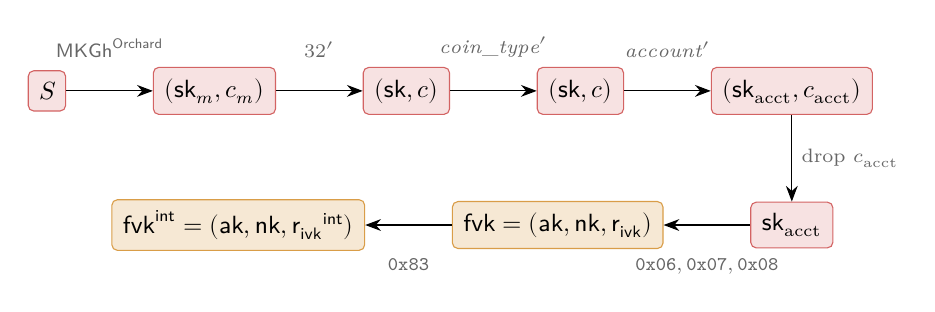
\begin{tikzpicture}[>={Stealth[length=2mm]},
  node distance=11mm and 11mm,
  key/.style={draw, rounded corners=2pt, inner sep=4pt, font=\small},
  spendk/.style={key, fill=tierspend!15, draw=tierspend!80},
  fullk/.style={key, fill=tierfull!20, draw=tierfull!85},
  elab/.style={font=\scriptsize, text=black!60, midway, above=3mm},
  blab/.style={font=\scriptsize, text=black!60, midway, below=3mm},
]
\node[spendk] (S) {$S$};
\node[spendk, right=of S] (M) {$(\mathsf{sk}_m, c_m)$};
\node[spendk, right=of M] (P) {$(\mathsf{sk}, c)$};
\node[spendk, right=of P] (CT) {$(\mathsf{sk}, c)$};
\node[spendk, right=of CT] (A) {$(\mathsf{sk}_{\mathrm{acct}}, c_{\mathrm{acct}})$};
\draw[->] (S) -- node[elab] {$\mathsf{MKGh}^{\mathsf{Orchard}}$} (M);
\draw[->] (M) -- node[elab] {$32'$} (P);
\draw[->] (P) -- node[elab] {$\mathit{coin\_type}'$} (CT);
\draw[->] (CT) -- node[elab] {$\mathit{account}'$} (A);
\node[spendk, below=of A] (SK) {$\mathsf{sk}_{\mathrm{acct}}$};
\draw[->] (A) -- node[right, font=\scriptsize, text=black!60] {drop $c_{\mathrm{acct}}$} (SK);
\node[fullk, left=of SK] (F) {$\fvk = (\aksym, \nksym, \rivk)$};
\node[fullk, left=of F] (FI) {$\fvk^{\mathsf{int}} = (\aksym, \nksym, \rivk^{\mathsf{int}})$};
\draw[->] (SK) -- node[blab] {$\mathtt{0x06}, \mathtt{0x07}, \mathtt{0x08}$} (F);
\draw[->] (F) -- node[blab] {$\mathtt{0x83}$} (FI);
\end{tikzpicture}
\caption{The deployed Orchard key path. The first horizontal arrow is
master-key generation; each subsequent arrow in the top row is one
$\mathsf{CKDsk}$ call (Definition~\ref{def:zip32-ckd}): a
$\mathsf{PRFexpand}$ invocation with lead byte $\mathtt{0x81}$, keyed by
the parent chain code. The chain code travels only as far as the account
node $(\mathsf{sk}_{\mathrm{acct}}, c_{\mathrm{acct}})$; the wallet layer
keeps the bare $\mathsf{sk}_{\mathrm{acct}}$, from which the external full
viewing key $\fvk$ (\emph{Ironwood Guide}, lead bytes
$\mathtt{0x06}/\mathtt{0x07}/\mathtt{0x08}$) and the internal
$\fvk^{\mathsf{int}}$ (Definition~\ref{def:zip32-internal}, lead byte
$\mathtt{0x83}$) both derive. Red marks spend capability, orange
full-viewing capability, per the series palette.}\label{fig:zip32-path}
\end{figure}

\paragraph{Deployed path derivation.} Function
\texttt{SpendingKey::from\_zip32\_seed(seed, coin\_type, account)} rejects
$\mathit{coin\_type} \ge 2^{31}$ with \texttt{Error::InvalidChildIndex},
runs \texttt{ExtendedSpendingKey::}\allowbreak\texttt{from\_path} over the three hardened
indices of Definition~\ref{def:zip32-path}, and returns only the $32$-byte
account spending key --- the chain code is discarded, so the wallet layer
retains no Orchard child-derivation capability below the account level.
Above it, \texttt{UnifiedSpendingKey::from\_seed} stores that plain
\texttt{SpendingKey}, and the unified full viewing key's Orchard component
is the \texttt{FullViewingKey} computed from it. The \textsf{zip32} crate types the path levels:
\texttt{AccountId} is a $31$-bit integer whose \texttt{TryFrom<u32>}
rejects values at or above $2^{31}$ and which always enters paths hardened,
and \texttt{ChildIndex} is hardened-only --- \texttt{from\_index} returns
\texttt{None} unless the hardened bit is set, and \texttt{hardened(v)}
asserts $v < 2^{31}$ and stores $v + 2^{31}$. A distinguished index
$\texttt{ChildIndex::PRIVATE\_USE} = \mathtt{0x7fffffff}'$ is reserved for
private-use subtrees; \textsf{zcashd}'s legacy Sapling account uses it, and
we find no Orchard use (ZIP-32, ``Sapling key path'';
\textsf{zip32}~0.2.0, \texttt{src/lib.rs}).

\subsection{From the account key to addresses: the layer already built}\label{sec:zip32-fvk}

Everything below $\mathsf{sk}_{\mathrm{acct}}$ is the hierarchy the
\emph{Ironwood Guide} constructs in ``The recipient: keys and addresses'', and
we do not
re-derive it: $\ask$, $\nksym$, $\rivk$ from $\mathsf{PRFexpand}$ lead
bytes $\mathtt{0x06}$, $\mathtt{0x07}$, $\mathtt{0x08}$ with the
$\mathrm{ToScalar}$/$\mathrm{ToBase}$ reductions and their bias analysis;
the sign-canonicalised $\aksym = [\ask]\,G^{\mathsf{SpendAuth}}$;
$\fvk = (\aksym, \nksym, \rivk)$;
$\ivk = \CommitIvk_{\rivk}(\Extract(\aksym), \nksym)$; the
$(\dk, \ovk)$ split of a single $\mathsf{PRFexpand}$ output with lead byte
$\mathtt{0x82}$; and the FF1 diversified addresses with default index $0$
(protocol specification \href{https://zips.z.cash/protocol/protocol.pdf\#orchardkeycomponents}{\S4.2.3}, ``Orchard Key Components'').

What ZIP-32 adds at the wallet level is the capability boundary of the full
viewing key. The holder of $\fvk$ obtains, for \emph{both} the external and
the internal scope of \S\ref{sec:zip32-internal}: the incoming viewing keys,
the diversifier keys and outgoing viewing keys, and hence every diversified
address of the account; the \emph{index} behind any of its addresses,
since the diversifier map is a keyed permutation and
$\mathsf{FF1\text{-}AES256}^{-1}_{\dk}(d)$ --- FF1
decryption under the empty tweak --- recovers the index; and the scope of any of its
addresses, by trying external then internal. Two contrasts with Sapling sharpen the picture
(ZIP-32, ``Orchard diversifier and OVK derivation''): the diversifier key
derives from the \emph{full viewing key} rather than the extended spending
key, so viewing capability suffices to locate an address's position in the
sequence; and all $2^{88}$ diversifiers are valid, so no rejection loop
exists and the default diversifier is $d_0$. What the full viewing key can
\emph{not} do: derive $\ask$, or derive any child account --- the former by
DL hardness for $\aksym=[\ask]G^{\mathsf{SpendAuth}}$, the latter because only
hardened derivation exists and no extended FVK is defined
(\S\ref{sec:zip32-hardened}). Finally, no mechanism derives an outgoing
viewing key per \emph{diversified address}: payments are sent from accounts,
with external or internal scope, not from individual addresses (ZIP-32,
``Orchard diversifier and OVK derivation'', citing the ZIP-316 rationale
``Usage of Outgoing Viewing Keys'').

\subsection{Internal keys: change and auto-shielding}\label{sec:zip32-internal}

The path of Definition~\ref{def:zip32-path} reserved no change level, so
the separation between externally visible receiving and wallet-internal
operations --- change outputs, and the auto-shielding of transparent funds
--- happens below the account instead: every account key yields a second,
\emph{internal} full viewing key. The mechanism was implemented in
\textsf{zcashd} as part of ZIP-316 support and applies to keys that are
children of the account level, i.e.\ account keys (ZIP-32, ``Orchard
internal key derivation'').

\begin{definition}[Orchard internal key derivation]\label{def:zip32-internal}
Given an external full viewing key $\fvk = (\aksym, \nksym, \rivk)$, let
$K := \mathrm{LE}_{256}(\rivk)$ and
\begin{gather*}
\rivk^{\mathsf{int}} := \mathrm{ToScalar}\bigl(\mathsf{PRFexpand}_{K}\bigl(
\mathtt{0x83} \,\|\, \mathrm{I2LEOSP}_{256}(\aksym) \,\|\,
\mathrm{I2LEOSP}_{256}(\nksym)\bigr)\bigr) \in \F_{p_{\Vesta}}, \\
\fvk^{\mathsf{int}} := (\aksym, \nksym, \rivk^{\mathsf{int}}),
\end{gather*}
i.e.\ $\mathsf{DeriveInternalFVK}^{\mathsf{Orchard}}$ modifies \emph{only}
$\rivk$ (ZIP-32, ``Orchard internal key derivation''; protocol
specification \href{https://zips.z.cash/protocol/protocol.pdf\#orchardkeycomponents}{\S4.2.3}). The downstream keys then follow the standard
FVK-level rules of the \emph{Ironwood Guide}, applied to
$\fvk^{\mathsf{int}}$:
$\ivk^{\mathsf{int}} := \CommitIvk_{\rivk^{\mathsf{int}}}(\Extract(\aksym), \nksym)$
and $(\dk^{\mathsf{int}}, \ovk^{\mathsf{int}})$ from the $\mathtt{0x82}$
split keyed by $\mathrm{LE}_{256}(\rivk^{\mathsf{int}})$. The
\emph{expanded internal spending key} is
$(\ask, \nksym, \rivk^{\mathsf{int}})$ --- the same $\ask$ --- and no
$32$-byte internal spending key exists (ZIP-32, ``Orchard internal key
derivation'').
\end{definition}

The shape is deliberately that of the $(\dk, \ovk)$ derivation: the same
key $K$, the same message body
$\mathrm{I2LEOSP}_{256}(\aksym) \,\|\, \mathrm{I2LEOSP}_{256}(\nksym)$,
a different lead byte. Its consequences: $\aksym$ and $\nksym$ are
unchanged (the protocol specification notes
$\aksym^{\mathsf{int}} = \aksym$ and $\nksym^{\mathsf{int}} = \nksym$,
\href{https://zips.z.cash/protocol/protocol.pdf\#orchardkeycomponents}{\S4.2.3}), so spend authorisation and nullifier derivation are common to
both scopes, while $\ivk$, $\dk$, and $\ovk$ are re-derived from
$\rivk^{\mathsf{int}}$. The construction does not explicitly enforce that
the two scopes' derived keys or addresses differ; equality would be a
negligible cryptographic collision, not an impossible case. Except with that
negligible probability, a note addressed under the internal scope does not
trial-decrypt under the external $\ivk$
(\emph{Ironwood Guide}, ``Delivery: the note reaches its owner''), which is
precisely the separation a wallet wants when it hands its external incoming
viewing key to a payment processor. Note that the internal FVK is
\emph{computable from} the external FVK --- the derivation consumes only
$(\aksym, \nksym, \rivk)$ --- so disclosing the full viewing key disclosed
both scopes all along; the boundary runs at the incoming-viewing tier, not
the full-viewing tier. Unlike its Sapling counterpart, the construction
does not rest on non-hardened derivation, which is undefined for Orchard
(ZIP-32, ``Orchard internal key derivation'').

Deployed, the \textsf{zip32} crate's \texttt{Scope} enum
$\{\texttt{External}, \texttt{Internal}\}$ names the two scopes and
\textsf{orchard} re-exports it; \texttt{FullViewingKey::rivk(Scope)},
\texttt{to\_ivk}, \texttt{to\_ovk}, and \texttt{derive\_internal} implement
Definition~\ref{def:zip32-internal}. The change
path is concrete: \textsf{zcash\_client\_backend} sends Orchard change to
\texttt{ufvk.orchard().address\_at(0u32, Scope::Internal)} --- the
internal-scope address at diversifier index $0$.

The transparent pool needs the same external/internal $\ovk$ split ---
its auto-shielding transactions carry shielded outputs whose outgoing
ciphertexts want a viewing key --- but P2PKH keys
(pay-to-public-key-hash: the output script pays to the hash of a single
public key) have no protocol-level $\ovk$ to scope, so ZIP-316
synthesises the pair.

\begin{definition}[Transparent internal and external OVK]%
\label{def:zip32-transparent-ovk}
For a transparent P2PKH account with BIP-32 account-level extended public
key $(c, pk)$ --- chain code $c$, keying $\mathsf{PRFexpand}$ as a
$256$-bit key, and $\mathsf{ser}(pk)$ the $33$-byte compressed public
key ---
\[
I_{\ovk} := \mathsf{PRFexpand}_{c}\bigl(\mathtt{0xd0} \,\|\,
\mathsf{ser}(pk)\bigr),
\qquad
\ovk_{\mathrm{external}} := I_{\ovk}[0..32),
\quad
\ovk_{\mathrm{internal}} := I_{\ovk}[32..64)
\]
(ZIP-316, \emph{Deriving Internal Keys}; lead byte in
Table~\ref{tab:prfexpand}).
\end{definition}

\begin{remark}[Byte-level normalisation between ZIP and code]
ZIP-32 writes the PRF key as the bit sequence
$\mathrm{I2LEBSP}_{256}(\rivk)$ where $\mathsf{PRFexpand}$ consumes bytes;
the code passes \texttt{rivk.to\_repr()}, the $32$-byte little-endian
encoding. The two are identical under the $\mathrm{LE}_{256}$ convention
this series uses, and we write $\mathrm{LE}_{256}$ throughout, as the
\emph{Ironwood Guide} already does. Likewise the $\aksym$ bytes fed to the
$\mathtt{0x82}$ and $\mathtt{0x83}$ messages are
\texttt{SpendValidatingKey::to\_bytes()}, the $32$-byte RedPallas point
encoding --- which, because key generation forces the sign bit to zero (the
canonicalisation of the \emph{Ironwood Guide}), coincides with
$\mathrm{I2LEOSP}_{256}(\Extract(\aksym))$, matching the specification's
$\mathrm{I2LEOSP}_{256}(\aksym)$ for
$\aksym \in \{0, \dots, p_{\Pallas}-1\}$ (protocol specification \href{https://zips.z.cash/protocol/protocol.pdf\#orchardkeycomponents}{\S4.2.3} and the
$\mathsf{AuthSignPublic}$ type). The $\nksym$ bytes are the base-field
representation.
\end{remark}

\subsection{Key validity and derivation failure}\label{sec:zip32-invalid}

\begin{definition}[Valid Orchard spending key]\label{def:zip32-validity}
A $32$-byte string $\mathsf{sk}$ is a \emph{valid} spending key iff all
three hold: (i) $\ask \ne 0$; (ii) the external
$\ivk = \CommitIvk_{\rivk}(\Extract(\aksym), \nksym) \notin \{0, \bot\}$;
(iii) the internal
$\ivk^{\mathsf{int}} = \CommitIvk_{\rivk^{\mathsf{int}}}(\Extract(\aksym),
\nksym) \notin \{0, \bot\}$. Function \texttt{SpendingKey::from\_bytes}
returns \texttt{None} exactly when one of the three fails, and the specification's
key-generation algorithm mandates exactly these three discard conditions
--- ``discard this key and repeat with a new $\mathsf{sk}$'' (protocol
specification \href{https://zips.z.cash/protocol/protocol.pdf\#orchardkeycomponents}{\S4.2.3}, ``Orchard Key Components'').
\texttt{FullViewingKey::from\_bytes} re-checks both scopes when parsing an
FVK from bytes.
\end{definition}

\begin{remark}[Derivation failure has no specified recovery]
ZIP-32 notes that a child spending key may yield an invalid external or
internal full viewing key ``with small probability'' (ZIP-32, ``Orchard
child key derivation'') but prescribes no wallet behaviour when it does;
the specification's ``repeat with a new $\mathsf{sk}$'' addresses a freshly
random key, not a fixed HD path, where there is nothing to redraw. The
deployed stack hard-errors: \texttt{master} and \texttt{derive\_child}
return \texttt{Err(Error::InvalidSpendingKey)},
\texttt{from\_path} propagates it, and \textsf{zcash\_keys} surfaces it as
\texttt{DerivationError::Orchard} (\textsf{orchard}, \texttt{src/zip32.rs};
\textsf{zcash\_keys}, \texttt{src/keys.rs}); no layer implements a
skip-to-next-index convention. This behaviour is normative in practice: an
account index at which derivation fails simply has no key, and no deployed
convention reassigns it. The event is negligibly rare --- neither ZIP-32
nor the specification quantifies ``small probability'', so
Proposition~\ref{prop:zip32-invalid} derives a bound --- and the gap is
theoretical.
\end{remark}

\begin{proposition}[Probability of an invalid key]\label{prop:zip32-invalid}
Model the $\mathsf{PRFexpand}$ outputs and the $\GroupHash$-derived
Sinsemilla generators as uniform and independent (the random-oracle model
in which the \emph{Ironwood Guide} analyses both primitives). A uniformly
random $32$-byte $\mathsf{sk}$ then fails the conditions of
Definition~\ref{def:zip32-validity} with probabilities
\[
\Pr[\ask = 0] \;<\; 2^{-254}, \qquad
\Pr\bigl[\ivk \in \{0, \bot\}\bigr] \;<\; 307\mathbin{\cdot}2^{-254}
\;<\; 2^{-245}
\quad \text{(per scope)},
\]
and is invalid with probability below $2^{-244}$.
\end{proposition}

\begin{proof}
The scalar $\ask$ is the $\mathrm{ToScalar}$ image of the $\mathtt{0x06}$
expansion (the conditional negation that canonicalises $\aksym$ preserves
zeroness), so $\ask = 0$ iff a uniform $512$-bit integer reduces to $0$
modulo $p_{\Vesta}$. Exactly $\lceil 2^{512}/p_{\Vesta} \rceil$ of the
$2^{512}$ inputs do, and $p_{\Vesta} > 2^{254}$ gives
$\lceil 2^{512}/p_{\Vesta} \rceil < 2^{258}$, hence
$\Pr[\ask = 0] < 2^{258} \cdot 2^{-512} = 2^{-254}$.

For $\ivk$, the two memberships separately. \emph{Zero}: conditioned on
the Sinsemilla hash not returning $\bot$, the commitment point is the hash
point plus $[\rivk]\,H_D$ --- the blinding term of the \emph{Ironwood
Guide}'s ``Sinsemilla: hash, commitment, and short forms'' --- uniform on the
$p_{\Vesta}$-element Pallas group when the blinding scalar is uniform
and $H_D\ne\mathcal O$. Here
$\rivk$ is the $\mathrm{ToScalar}$ image of a uniform $512$-bit string, so
the probability of any particular scalar is at most
$\lceil 2^{512}/p_{\Vesta}\rceil/2^{512} < 2^{-254}$. The extractor sends only
the identity to $0$, because $y^2 = 0^3 + 5$ has no solution in
$\F_{p_{\Pallas}}$ --- $5$ is a non-square there (protocol specification
\href{https://zips.z.cash/protocol/protocol.pdf\#concreteextractorpallas}{\S5.4.9.7}, note) --- so $\Pr[\ivk = 0] < 2^{-254}$.
\emph{Bottom}: the $\bot$ output arises only inside the Sinsemilla hash,
since the blinding addition is complete (\href{https://zips.z.cash/protocol/protocol.pdf\#concretesinsemillacommit}{\S5.4.8.4}). On the $510$-bit
$\CommitIvk$ message --- two $255$-bit field encodings,
$\lceil 510/10 \rceil = 51$ ten-bit chunks --- the hash performs
$2 \cdot 51 = 102$ incomplete additions (\href{https://zips.z.cash/protocol/protocol.pdf\#concretesinsemillahash}{\S5.4.1.9}). Each fails only when
one operand is the identity or shares the other's $x$-coordinate.
To avoid assuming uniformity after conditioning on prior success,
consider each round's unconditioned complete-law expression
$(A+P)+A$. Conditional on the message and table points, its accumulator
is $A=[2^i]Q+C_i$, uniform as the independent generator $Q$ varies.
For $P\ne\mathcal O$, exceptional incomplete additions require
$A\in\{\mathcal O,P,-P,-P/2\}$; the separate event
$P=\mathcal O$ costs at most $1/p_{\Vesta}$. Thus the $51$ rounds
cost at most $255/p_{\Vesta}$ by a union bound, without independence
between rounds. Including the negligible event that the blinding base
is the identity still fits the conservative bound
$\Pr[\ivk\in\{0,\bot\}] < 307\cdot2^{-254} < 2^{-245}$ per scope.
The internal scope
repeats the argument with the independent $\rivk^{\mathsf{int}}$ (the
$\mathtt{0x83}$ expansion). In total,
$\Pr[\mathsf{sk}\ \text{invalid}] < (1 + 2 \cdot 307) \cdot 2^{-254} <
2^{10} \cdot 2^{-254} = 2^{-244}$.
\end{proof}

The bound makes ZIP-32's ``small probability'' concrete: below $2^{-244}$
per derived key, and below $2^{-242}$ for the union over the four nodes of
the standard account path (master included,
Definition~\ref{def:zip32-master}). This is a random-oracle-model bound,
including randomness over the generators, not a measured frequency for
the one deployed set of fixed generators. Moreover, a concrete input
exhibiting $\bot$ would
constitute a nontrivial discrete-log relation among the Sinsemilla
generators (\emph{Ironwood Guide}, the Sinsemilla collision-resistance
proof), so none is expected ever to be observed.

\subsection{Fingerprints and tags}\label{sec:zip32-fingerprints}

Two identifiers name objects of this section without revealing them; both
are BLAKE2b-256 digests with dedicated personalisations.

\begin{definition}[Orchard FVK fingerprint and tag]\label{def:fvk-fingerprint}
For a full viewing key $\fvk = (\aksym, \nksym, \rivk)$, the
\emph{fingerprint} is
\begin{align*}
\mathsf{FVFP}(\fvk) &:= \mathrm{BLAKE2b\text{-}256}\bigl(
\texttt{``ZcashOrchardFVFP''},\ \fvk_{\mathrm{raw}}\bigr), \\
\fvk_{\mathrm{raw}} &:= \mathrm{I2LEOSP}_{256}(\aksym) \,\|\,
\mathrm{I2LEOSP}_{256}(\nksym) \,\|\, \mathrm{I2LEOSP}_{256}(\rivk),
\end{align*}
the digest of the $96$-byte raw FVK encoding $\fvk_{\mathrm{raw}}$
(protocol specification \href{https://zips.z.cash/protocol/protocol.pdf\#orchardfullviewingkeyencoding}{\S5.6.4.4}). The \emph{tag} is its first $4$ bytes
and MUST NOT be assumed unique; the master key's parent tag is the $4$
zero bytes (ZIP-32,
``Orchard Full Viewing Key Fingerprints and Tags''). Deployed as
\texttt{FvkFingerprint} and \texttt{FvkTag}; child derivation stamps each
child with \texttt{parent\_fvk\_tag} $=$ the tag of the parent's FVK.
\end{definition}

\begin{definition}[Seed fingerprint]\label{def:seed-fingerprint}
For a seed $S$ of $32$ to $252$ bytes, with $[\mathrm{length}(S)]$ its
single length byte,
\[
\mathsf{SeedFP}(S) := \mathrm{BLAKE2b\text{-}256}\bigl(
\texttt{``Zcash\_HD\_Seed\_FP''},\ [\mathrm{length}(S)] \,\|\, S\bigr);
\]
the string form is Bech32m (the checksummed base-32 string encoding of
BIP-350: a human-readable part, a separator \texttt{1}, and base-32 data
characters ending in a six-character checksum) with human-readable part
\texttt{zip32seedfp}, and no short tag is defined; the length prefix was
chosen to match \textsf{zcashd}'s implementation (ZIP-32, ``Seed
Fingerprints''). Deployed, \texttt{SeedFingerprint::from\_seed} returns
\texttt{None} outside the $32..252$-byte bounds, and \textsf{zcash\_client\_sqlite} uses the
fingerprint to bind each stored account to the seed that produced it.
\end{definition}

\subsection{Extended-key encoding and test vectors}\label{sec:zip32-encoding}

\begin{definition}[Orchard extended spending key encoding]\label{def:xsk-encoding}
An extended spending key at depth $\mathsf{depth}$, child index $i$
(hardened offset included), with parent tag $\mathsf{tag}_{\mathrm{par}}$,
serialises as the $73$-byte string
\[
\mathsf{xsk} := \mathrm{I2LEOSP}_{8}(\mathsf{depth}) \,\|\,
\mathsf{tag}_{\mathrm{par}} \,\|\, \mathrm{I2LEOSP}_{32}(i) \,\|\, c \,\|\,
\mathsf{sk}
\qquad (1 + 4 + 4 + 32 + 32 \text{ bytes}),
\]
with the master key at depth $0$, tag $\mathtt{0x00000000}$, index $0$.
The Bech32 human-readable parts are
\texttt{secret-orchard-extsk-main} (Mainnet) and
\texttt{secret-orchard-extsk-test} (Testnet) (ZIP-32, ``Orchard extended
spending keys'').
\end{definition}

ZIP-32 defines this encoding ``for completeness'' and expects most wallets
to expose only the plain $\mathsf{sk}$ encoding of the protocol
specification (\href{https://zips.z.cash/protocol/protocol.pdf\#orchardspendingkeyencoding}{\S5.6.4.5}) --- consistent with the deployed stack, which
discards the chain code at the account level
(\S\ref{sec:zip32-path}). Indeed we find \emph{no} deployed
\textsf{librustzcash} code path that emits or parses the Bech32 form: the
$73$-byte layout is exercised only by the \textsf{orchard} crate's
embedded test-vector checks, and \textsf{zcash\_keys} stores the raw
spending key inside the unified spending key encoding (\textsf{orchard},
\texttt{src/zip32.rs}, \texttt{src/test\_vectors/zip32.rs};
\textsf{zcash\_keys}, \texttt{src/keys.rs}). We classify the encoding as
specified but unused in the scanned stack.

\begin{remark}[Test vectors]
The ZIP-32 Orchard vectors live in \textsf{zcash-test-vectors} under
\texttt{orchard\_\allowbreak zip32}; the \textsf{orchard} crate embeds four of them ---
the nodes $m$, $m/1'$, $m/1'/2'$, $m/1'/2'/3'$ from the $32$-byte seed
$\mathtt{0x00}, \dots, \mathtt{0x1f}$ --- each giving $\mathsf{sk}$, $c$,
the $73$-byte $\mathsf{xsk}$, and the FVK fingerprint (ZIP-32, ``Test
Vectors''; \textsf{orchard}, \texttt{src/test\_vectors/zip32.rs},
\texttt{src/zip32.rs}). They do \emph{not} cover the standard path of
Definition~\ref{def:zip32-path}. Separate key-component vectors
($\mathsf{sk} \to \ask, \aksym, \nksym, \rivk, \ivk$ and the internal-scope
components) sit in \texttt{src/test\_vectors/keys.rs}, exercised by the
\texttt{keys.rs} tests.
\end{remark}

\begin{example}[The standard path, worked]\label{ex:zip32-standard-path}
No published vector covers the path of Definition~\ref{def:zip32-path}, so
we compute one, from the embedded vectors' seed
$S = \mathtt{0x00}, \dots, \mathtt{0x1f}$, for Mainnet
($\mathit{coin\_type} = 133$) and account $0$:
\begin{center}
\small
\begin{tabular}{@{}lll@{}}
\toprule
$m$ & $\mathsf{sk}$ &
  \texttt{7eee3c1017870990a3dd6891b82f80be8976c1e7dc20d60817a5e88e8b2cd4b8} \\
 & $c$ &
  \texttt{ab8b7a00509ef20e469b5292b61d474b7cffcb1657924cda720250ae40526677} \\
\addlinespace
$m/32'$ & $\mathsf{sk}$ &
  \texttt{93af0a87c2e4704d8825e145557c6a5d4dcbc9016170e276a2080a2dc9eb0f87} \\
 & $c$ &
  \texttt{6e1e808d410d6d1f84e62e67c8b60e80e5ee4de5021d575c0433a625d609c45c} \\
\addlinespace
$m/32'/133'$ & $\mathsf{sk}$ &
  \texttt{149fcee594a2a03de277ab919f22611d0ef6aa8e8e9a0bef32f01a0bcb0e8c4c} \\
 & $c$ &
  \texttt{07d13fdeccd21da16b467f8e785edc32f74ceeb541bede0394647f10fdb7114f} \\
\addlinespace
$m/32'/133'/0'$ & $\mathsf{sk}$ &
  \texttt{b67d8d87cab9189500afb45dbca9f92c924c1de9d9ee1451be4a78313cb223b4} \\
 & $c$ &
  \texttt{7ff0a6392e144d4c8f45bca21fb7827b508446ac069890aefbebbe388b7a84c0} \\
\bottomrule
\end{tabular}
\end{center}
The bottom $\mathsf{sk}$ is exactly what
\texttt{SpendingKey::from\_zip32\_seed} returns for $(S, 133, 0)$; the
bottom $c$ is what it discards. The account key's FVK fingerprint
(Definition~\ref{def:fvk-fingerprint}) is
\begin{center}
\small
\texttt{da8dab741dc4f6ff8964fbaa8840270caf47d286e9a0722e6c89e7f2c38189d5}
\end{center}
(tag $\mathtt{da8dab74}$), its parent's fingerprint begins
$\mathtt{7010c19b}$, and the account's $73$-byte encoding of
Definition~\ref{def:xsk-encoding} is therefore
\[
\mathsf{xsk} = \mathtt{03} \,\|\, \mathtt{7010c19b} \,\|\,
\mathtt{00000080} \,\|\, c \,\|\, \mathsf{sk},
\qquad \mathtt{00000080} = \mathrm{I2LEOSP}_{32}(0'),
\]
with $c$ and $\mathsf{sk}$ the bottom table row. The numbers are
script-computed per the series conventions: a standalone reimplementation
of $\mathsf{MKGh}^{\mathsf{Orchard}}$ and $\mathsf{CKDsk}$ first
reproduces all four embedded vectors byte for byte ($\mathsf{sk}$, $c$,
$\mathsf{xsk}$); the \textsf{orchard} crate, driven as a library,
reproduces their FVK fingerprints, returns the same account $\mathsf{sk}$
from \texttt{from\_zip32\_seed}, and validates every node above per
Definition~\ref{def:zip32-validity}.
\end{example}

\subsection{The \texorpdfstring{$\mathsf{PRFexpand}$}{PRFexpand} lead-byte
registry}\label{sec:zip32-registry}

One PRF underlies every derivation above and in the \emph{Ironwood Guide},
but domain separation is per PRF \emph{key}, not protocol-wide: under a
fixed key, distinct lead bytes provide domain-separated pseudorandom
outputs, while separate consumers may reuse a byte under different
keys. Sapling derives $\rcm$ and $\mathsf{esk}$ from lead bytes
$\mathtt{0x04}$ and $\mathtt{0x05}$ with no $\rho$ suffix --- the
assignment swapped relative to Orchard's, which the specification
attributes to an oversight (protocol specification \href{https://zips.z.cash/protocol/protocol.pdf\#orchardsend}{\S4.7.3}, note) --- and
the Sapling
instantiation of ZIP-32 intentionally reuses
$\mathtt{0x00}$--$\mathtt{0x02}$ from the Sapling key components under a
different key. Table~\ref{tab:prfexpand} collects the accounting for the
Orchard, Orchard-ZIP-32, and ZIP-316 bytes this series constructs; the
Sapling-only bytes ($\mathtt{0x00}$--$\mathtt{0x03}$,
$\mathtt{0x10}$--$\mathtt{0x18}$, of which
\S\ref{sec:addresses-diversified} cites $\mathtt{0x10}$ and
$\mathtt{0x16}$) are accounted in the specification's list (protocol
specification, the $\mathsf{PRF}^{\mathsf{expand}}$ accounting under
\href{https://zips.z.cash/protocol/protocol.pdf\#concreteprfs}{``Pseudo Random Functions''} and \href{https://zips.z.cash/protocol/protocol.pdf\#orchardkeycomponents}{\S4.2.3}; ZIP-32). The Sprout
instantiation of ZIP-32 reserves the lead byte $\mathtt{0x80}$, the
personalisation \texttt{``ZcashIP32\_Sprout''}, and the HRPs
\texttt{zxsprout}/\texttt{zxtestsprout} --- values the ZIP says SHOULD NOT
be used in future Zcash-related specifications (ZIP-32, ``Values reserved
due to previous specification for Sprout''). All Orchard and ZIP-32
constants of those derivations match between the specification text and
\textsf{zcash\_spec}~0.2.1 --- the version locked by both the
\textsf{orchard} and \textsf{librustzcash} workspaces
(\texttt{Cargo.lock} in each; likewise \textsf{zip32}~0.2.0).
The additional Ironwood $\mathtt{0x0B}$ derivation is implemented
directly in \textsf{orchard}~0.15.0, \texttt{src/note.rs}, not in that
older \textsf{zcash\_spec} registry.

\begin{table}[htbp]
\centering
\small
\begin{tabular}{@{}llll@{}}
\toprule
Lead byte & PRF key & Message after the lead byte & Output \\
\midrule
$\mathtt{0x04}$ & $\mathsf{rseed}$ & $\rho$ & $\mathsf{esk}$ \\
$\mathtt{0x05}$ & $\mathsf{rseed}$ & $\rho$ & legacy $\rcm$ \\
$\mathtt{0x06}$ & $\mathsf{sk}$ & --- & $\ask$ \\
$\mathtt{0x07}$ & $\mathsf{sk}$ & --- & $\nksym$ \\
$\mathtt{0x08}$ & $\mathsf{sk}$ & --- & $\rivk$ \\
$\mathtt{0x09}$ & $\mathsf{rseed}$ & $\rho$ & $\psi$ \\
$\mathtt{0x0B}$ & $\mathsf{rseed}$ & $\mathsf{pre\_rcm}[1..137)$ & Ironwood $\rcm$ \\
$\mathtt{0x80}$ & \multicolumn{3}{l}{Sprout ZIP-32 child (reserved; SHOULD NOT reuse)} \\
$\mathtt{0x81}$ & $c_{\mathrm{par}}$ &
  $\mathsf{sk}_{\mathrm{par}} \,\|\, \mathrm{I2LEOSP}_{32}(i)$ &
  $\mathsf{sk}_i \,\|\, c_i$ \\
$\mathtt{0x82}$ & $\mathrm{LE}_{256}(\rivk)$ (per scope) &
  $\aksym \,\|\, \nksym$ & $\dk \,\|\, \ovk$ \\
$\mathtt{0x83}$ & $\mathrm{LE}_{256}(\rivk)$ & $\aksym \,\|\, \nksym$ & $\rivk^{\mathsf{int}}$ \\
$\mathtt{0xAB}$ & \multicolumn{3}{l}{ad-hoc ZIP-32 child (deprecated)} \\
$\mathtt{0xAC}$ & \multicolumn{3}{l}{registered ZIP-32 child} \\
$\mathtt{0xD0}$ & $c$ (chain code) & $\mathsf{ser}(pk)$ &
  $\ovk_{\mathrm{ext}} \,\|\, \ovk_{\mathrm{int}}$ \\
\bottomrule
\end{tabular}
\caption{Lead-byte registry of $\mathsf{PRFexpand}$ messages. Field
arguments use $\mathrm{I2LEOSP}_{256}$; points use their compressed
encodings (the canonical $\aksym$ encoding coincides with its
$x$-coordinate encoding). Here $\rho$ is the
$32$-byte nullifier of the Action's spent note (\emph{Ironwood Guide},
``Delivery: the note reaches its owner''). Rows
$\mathtt{0x04}$--$\mathtt{0x09}$ are constructed in the \emph{Ironwood
Guide} and carry the Orchard meanings of $\mathtt{0x04}$/$\mathtt{0x05}$.
The $\mathtt{0x0B}$ row uses the $137$-byte $\mathsf{pre\_rcm}$
defined in that volume's ``The note seed: Ironwood derivations (lead
byte $\mathtt{0x03}$)'', with its
first byte removed because the column already lists it (ZIP-2005).
Sapling reuses both bytes, without the $\rho$ suffix and with the outputs
swapped ($\mathtt{0x04} \to \rcm$, $\mathtt{0x05} \to \mathsf{esk}$),
under its own per-note $\mathsf{rseed}$ keys (protocol specification
\href{https://zips.z.cash/protocol/protocol.pdf\#orchardsend}{\S4.7.3}, note). Rows $\mathtt{0x81}$ and $\mathtt{0x83}$ are constructed
in
Definitions~\ref{def:zip32-ckd} and~\ref{def:zip32-internal};
$\mathtt{0xD0}$ in Definition~\ref{def:zip32-transparent-ovk};
$\mathtt{0x80}$, $\mathtt{0xAB}$, $\mathtt{0xAC}$ belong
to other subsystems (ZIP-32) and appear for the completeness of
the accounting.}\label{tab:prfexpand}
\end{table}

\section{Diversified and unified addresses (ZIP-316)}\label{sec:addresses}

An address layer must reconcile two demands that pull apart. Each payee
should receive their own address, mutually unlinkable with every other ---
yet all of them spendable by one key and recoverable from one seed; each
shielded protocol solves this with \emph{diversified addresses}. And Zcash
is several protocols at once: transparent, Sapling, and Orchard receivers
coexist, each with its own format, so a recipient wants to hand a sender
\emph{one} string from which the sender's wallet picks the best receiver
both sides support; ZIP-316 solves this above the protocols with the
\emph{unified} container encodings. The \emph{Ironwood Guide} (``The recipient:
keys and addresses'') already constructs the
Orchard-side machinery --- the key tiers, the FF1-AES256 diversifier map
$d := \mathsf{FF1\text{-}AES256}_{\dk}(d_{\mathrm{plain}})$, the
diversified base
$\gd = \GroupHash^{\Pallas}(\mathtt{z.cash:Orchard\text{-}gd}, d)$, and the
rationale for a keyed permutation over the index space --- and we cite it
throughout. This section adds what the wallet layer builds on top: the
index discipline shared across Sapling, Orchard, and transparent
derivation, the raw and unified encodings, viewing-key containers, and the
deployed address-generation code.

At \textsf{zips} \texttt{ad30e59}, ZIP-316 is organised into revisions:
Revision~0 is
Active and is what the deployed stack implements; Revision~1 was withdrawn;
Revision~2 is a Draft (ZIP-316, \emph{Revisions}). This volume documents
Revision~0 and states Revision~2 in \S\ref{sec:addresses-r2}, classified
\emph{specified, not deployed}; its reference implementation is
\textsf{librustzcash} PR~\#2199, absent from both the baseline and the
2026-08-30 \texttt{91f448b5} snapshot.
Deployed-behaviour claims below are verified against \textsf{librustzcash}
commit \texttt{e30517e4} --- the volume's baseline
(\S\ref{sec:zip321-crate}) --- and the crates-io releases
\textsf{zcash\_spec}~0.2.1, \textsf{zip32}~0.2.0,
\textsf{sapling-crypto}~0.7.0, and \textsf{orchard}~0.15.0 (exact versions
pinned by the \textsf{librustzcash} workspace \texttt{Cargo.lock}); ZIP
text is
quoted from the \textsf{zips} repository at commit \texttt{c6b7035}.

\subsection{Accounts: ZIP-32 key paths and wallet seeds}\label{sec:addresses-accounts}

Every address below hangs off an \emph{account}, a node of the ZIP-32
hierarchical-deterministic key tree. Sapling and Orchard share the path
shape
\[
m \,/\, \mathtt{purpose}' \,/\, \mathtt{coin\_type}' \,/\,
\mathtt{account}',
\]
with $\mathtt{purpose} = 32$ (hardened index $\mathtt{0x80000020}$), the SLIP-44 coin
type ($133$ on mainnet, $1$ on all testnets), the account index counting
from $0$, and every level hardened (ZIP-32, \emph{Key path levels};
\emph{Sapling key path}; \emph{Orchard key path}; deployed constants in
\textsf{zcash\_protocol}, \texttt{constants/}). Two absences are
deliberate. There is no change level: shielded change pays the wallet's own
address and is indistinguishable from any other output, so the transparent
external/internal split buys nothing (ZIP-32, \emph{Key path levels}). And
there is no non-hardened tail: Orchard ZIP-32 defines hardened-only
derivation, instantiated with
$\mathsf{MKGDomain} = \texttt{"ZcashIP32Orchard"}$ and
$\mathsf{CKDDomain} = \mathtt{0x81}$ over the extended spending key
$(\mathsf{sk}, c)$; a child may, with small probability, yield a spending
key whose external or internal full viewing key is invalid, in which case
derivation at that index simply fails --- ZIP-32 prescribes no recovery,
and the deployed stack surfaces an error (\S\ref{sec:zip32-invalid};
ZIP-32, \emph{Specification: Orchard key derivation}). Wallets MUST
support this path for accounts $0$ to
$2^{31}-1$ and MUST support generating each account's default payment
address; a stream of diversified addresses MAY be supported (ZIP-32,
\emph{Key path levels}; \emph{Sapling key path}; \emph{Orchard key path}).
The seed feeding the tree MUST be $32$--$252$ bytes with at least $256$
bits of entropy: an attack on a lower-entropy mnemonic can be run against
many wallets at once, by matching derived addresses and viewing keys
against observed ones (ZIP-32, \emph{Specification: Wallet seeds}).

\subsection{Diversified addresses}\label{sec:addresses-diversified}

A diversified address multiplies addresses without multiplying keys: one
incoming viewing key $\ivk$, one diversifier key $\dk$, and one $88$-bit
\emph{diversifier} $d$ per address. The \emph{Ironwood Guide} (``The recipient:
keys and addresses'') constructs the map and its
design rationale --- a keyed permutation of the index space, rather than a
hash or a random draw; the wallet layer fixes the index discipline that
ZIP-32 shares between Sapling and Orchard.

\begin{definition}[Diversifier derivation, Sapling and Orchard]\label{def:diversifier-derivation}
For an account's diversifier key $\dk$, the diversifier at
\emph{diversifier index} $j$ is
\[
d_j := \mathsf{FF1\text{-}AES256.Encrypt}\bigl(\dk,\ \texttt{""},\
\mathrm{LE}_{88}(j)\bigr),
\qquad j \in \{0, \dots, 2^{88}-1\},
\]
where $\mathsf{FF1\text{-}AES256}$ is NIST SP 800-38G FF1 with a $256$-bit
AES key, radix $2$, $\mathit{minlen} = \mathit{maxlen} = 88$, the tweak
always the empty string, and $\mathrm{LE}_{88}(j)$ (the ZIP's
$\mathrm{I2LEBSP}_{88}$) the index's $88$-bit little-endian bit encoding;
input and output are $88$-bit sequences. The
protocol specification abbreviates the keyed permutation as
$\mathrm{PRP}^{d}_{K}(d) := \mathsf{FF1\text{-}AES256}_K(\texttt{""}, d)$
(ZIP-32, \emph{Sapling diversifier derivation}; \emph{Orchard diversifier
and OVK derivation}; protocol specification \href{https://zips.z.cash/protocol/protocol.pdf\#concreteprps}{\S5.4.4}, \emph{Pseudo Random
Permutations}).
\end{definition}

The Orchard diversified payment address at index $j$ is then
\[
d := \mathrm{PRP}^{d}_{\dk}\bigl(\mathrm{LE}_{88}(j)\bigr),
\qquad
\gd := \mathsf{DiversifyHash}^{\mathsf{Orchard}}(d),
\qquad
\pkd := [\ivk]\,\gd,
\]
the pair $(d, \pkd)$, with the address at index $0$ the \emph{default}
diversified payment address; the last step is the key-agreement
$\mathsf{KA^{Orchard}.DerivePublic}$ of the protocol specification, and the
\emph{Ironwood Guide} constructs all three maps. Diversifier indices SHOULD
NOT be chosen at random, and an address generator MAY encode recoverable
information in the index --- the $\dk$ holder recovers it by FF1 decryption
(protocol specification \href{https://zips.z.cash/protocol/protocol.pdf\#orchardkeycomponents}{\S4.2.3}, \emph{Orchard Key Components}).

The deployed cipher is the \textsf{fpe} crate's \texttt{FF1<Aes256>} at
radix~$2$; the \textsf{orchard} crate pins \textsf{fpe}~0.6 in its
\texttt{Cargo.toml}. Both
protocols encrypt the index bytes \texttt{j.as\_bytes()} wrapped as a
\texttt{BinaryNumeralString} via \texttt{from\_bytes\_le} --- the $11$-byte
little-endian index with bits least-significant-first within each byte,
which is exactly $\mathrm{I2LEBSP}_{88}(j)$ --- under the empty tweak, and
convert the $88$-bit output back with \texttt{to\_bytes\_le}
into the $11$-byte diversifier, exactly $\mathrm{LEBS2OSP}_{88}$.

The permutation earns its keep quantitatively. An $88$-bit diversifier is
too short to be cryptographically unguessable at the $128$-bit security
level, and diversifiers chosen at random begin to collide by the birthday
bound as the number of draws approaches $2^{44}$; a keyed permutation
reaches the full $2^{88}$ range with no repetition, provided the input
index never repeats for a given node (protocol specification \href{https://zips.z.cash/protocol/protocol.pdf\#concretediversifyhash}{\S5.4.1.6},
notes). The remaining rationale --- per-account sequences pseudorandom and
mutually uncorrelated, and the issue-count leak a bare counter would cause
--- is the \emph{Ironwood Guide}'s diversifier construction, cited above.

\begin{remark}[FF1 parameter security]\label{rem:ff1-security}
The property the design requires is that FF1-AES256, with the tweak fixed
to the empty string, is a secure pseudo-random permutation. As
parameterized here --- radix $2$, an $88$-bit domain, $10$ rounds per NIST
SP 800-38G --- it is unaffected by the DKLS2020 attacks on small-domain
FF1: at their parameters $r = 5$ (half the number of rounds) and $n = 44$
(half the domain size in bits), the distinguishing attack has
data complexity $2^{2n((r-1)-1/2)-n} = 2^{264}$ and time complexity
$2^{2n((r-1)-1/2)} = 2^{308}$, no better than brute-forcing the $256$-bit
key (protocol specification \href{https://zips.z.cash/protocol/protocol.pdf\#concreteprps}{\S5.4.4}).
\end{remark}

\begin{definition}[Diversifier validity and default diversifiers]\label{def:diversifier-validity}
For Sapling,
\[
\mathsf{DiversifyHash}^{\mathsf{Sapling}}(d) :=
\mathsf{GroupJHash^{URS}}\bigl(\texttt{"Zcash\_gd"},\
\mathrm{LEBS2OSP}_{88}(d)\bigr),
\]
valued in the prime-order subgroup of Jubjub --- Sapling's elliptic
curve, carrying its keys and commitments as Pallas carries Orchard's ---
excluding zero, or $\bot$; the diversifier $d_j$ is \emph{valid} iff the
result is not $\bot$, which for a
given $\dk$ holds for approximately half of all indices $j$. The Sapling
\emph{default diversifier} is $d_j$ for the least nonnegative $j$ yielding
a valid diversifier, and a Sapling account has approximately
$2^{87}$ payment addresses (ZIP-32, \emph{Sapling diversifier derivation};
\emph{Sapling key path}). For Orchard, with
$P := \GroupHash^{\Pallas}(\mathtt{z.cash:Orchard\text{-}gd},
\mathrm{LEBS2OSP}_{88}(d))$,
\[
\mathsf{DiversifyHash}^{\mathsf{Orchard}}(d) :=
\begin{cases}
\GroupHash^{\Pallas}(\mathtt{z.cash:Orchard\text{-}gd}, \texttt{""})
  & \text{if } P = \mathcal{O}, \\
P & \text{otherwise,}
\end{cases}
\]
which never returns $\bot$: every one of the $2^{88}$ Orchard diversifiers
is valid, the default diversifier is $d_0$, and an account has exactly
$2^{88}$ payment addresses (protocol specification \href{https://zips.z.cash/protocol/protocol.pdf\#concretediversifyhash}{\S5.4.1.6}; ZIP-32,
\emph{Orchard diversifier and OVK derivation}; \emph{Orchard key path}).
\end{definition}

The totality of the Orchard hash --- and why it removes Sapling's
try-the-next-index rejection loop --- is discussed in the \emph{Ironwood
Guide} (``The recipient: keys and addresses''). The residual
Sapling failure rate of $\tfrac12$ per index is not a curiosity: it
resurfaces when a single index must serve several protocols at once
(\S\ref{sec:addresses-ua-from-uivk}).

The two protocols also place $\dk$ at different depths of the key tree. In
Sapling the diversifier key is a component of the \emph{extended spending
key}, derived down the ZIP-32 tree beside the spending authority:
\[
\dk_m := \mathrm{truncate}_{32}\bigl(
\mathsf{PRFexpand}_{\mathsf{sk}_m}([\mathtt{0x10}])\bigr),
\qquad
\dk_i := \mathrm{truncate}_{32}\bigl(
\mathsf{PRFexpand}_{I_L}([\mathtt{0x16}] \,\|\, \dk_{\mathrm{par}})\bigr),
\]
where $I_L$ is the ZIP-32 child-derivation entropy (ZIP-32, \emph{Sapling
master key generation}; \emph{Sapling child key derivation}). Orchard
instead derives $\dk$ directly from the full viewing key
$(\aksym, \nksym, \rivk)$, as one half of a single $\mathsf{PRFexpand}$
output whose other half is $\ovk$:
\[
\begin{gathered}
R := \mathsf{PRFexpand}_{\mathrm{LE}_{256}(\rivk)}\bigl(\mathtt{0x82}
\,\|\, \mathrm{I2LEOSP}_{256}(\aksym) \,\|\,
\mathrm{I2LEOSP}_{256}(\nksym)\bigr), \\
\dk := R[0..32), \qquad \ovk := R[32..64),
\end{gathered}
\]
the derivation the \emph{Ironwood Guide} types in full
($\mathsf{PRFexpand}_K(t)$ is BLAKE2b-512 with personalisation
\texttt{Zcash\_ExpandSeed} over $K \,\|\, t$; ZIP-32, \emph{Conventions};
protocol specification \href{https://zips.z.cash/protocol/protocol.pdf\#orchardkeycomponents}{\S4.2.3}). The consequence is capability parity with
a simpler key structure: any holder of the Orchard full viewing key can
determine the position of any diversifier in the account's sequence, as in
Sapling only a holder of the \emph{extended} full viewing key can (ZIP-32,
\emph{Orchard diversifier and OVK derivation}).

\begin{remark}[Reuse of $\rivk$]\label{rem:rivk-reuse}
The randomizer $\rivk$ serves twice: as the $\CommitIvk$ trapdoor and as
the $\mathsf{PRFexpand}$ key deriving $\dk$ and $\ovk$. If $\dk$ or $\ovk$
is known to an adversary, this reuse prevents proving \emph{perfect} hiding
for $\CommitIvk$ in this context, and modelling $\mathsf{PRFexpand}$ merely
as a PRF is insufficient; the specification instead makes a joint
assumption on Pallas scalar multiplication and $\mathsf{PRFexpand}$
(protocol specification \href{https://zips.z.cash/protocol/protocol.pdf\#orchardkeycomponents}{\S4.2.3}, security note).
\end{remark}

Inverting the permutation recovers the index:
\[
j = \mathsf{FF1\text{-}AES256.Decrypt}\bigl(\dk,\ \texttt{""},\ d\bigr).
\]
Decryption alone proves nothing about ownership: every valid diversifier
decrypts to \emph{some} index under \emph{every} diversifier key
(\textsf{sapling-crypto}~0.7.0, \texttt{src/zip32.rs}, doc comment: ``all
valid diversifiers can be produced by all diversifier keys''), so the
ownership test re-derives the address at the decrypted index under the
candidate $\ivk$ and compares it with the given address. Deployed: the
method \texttt{DiversifierKey::diversifier\_index} performs the raw FF1
decryption in both protocols, and the checked variants are the Orchard
\texttt{IncomingViewingKey::diversifier\_index} and the Sapling
\texttt{IncomingViewingKey::decrypt\_diversifier}.

\begin{remark}[Unlinkability, and an oracle to avoid]\label{rem:unlinkability}
The security requirement: given two randomly selected shielded payment
addresses of \emph{different} spend authorities and a third address
derivable from either, all three using different diversifiers, it is not
possible to tell from which of the two authorities the third address
derives. For Sapling this holds under DDH on the Jubjub prime-order
subgroup when $\mathsf{GroupJHash}$ is modelled as a random oracle, via
IK-CPA key privacy of ElGamal; the specification applies the same property
and notes to Orchard (protocol specification \href{https://zips.z.cash/protocol/protocol.pdf\#concretediversifyhash}{\S5.4.1.6}). One pitfall is
normative: an implementation SHOULD avoid providing a
\emph{chosen-diversifier} oracle --- deriving a new address for a given
$\ivk$ at an adversary-supplied diversifier --- since such an oracle
trivially breaks unlinkability for the other diversified addresses of that
$\ivk$ (same section, final note).
\end{remark}

\subsection{Raw encodings}\label{sec:addresses-raw}

An Orchard shielded payment address encodes raw in $43$ bytes,
\[
\mathrm{LEBS2OSP}_{88}(d) \,\|\, \pkd^\star,
\]
the $11$-byte diversifier followed by the $32$-byte star-encoding of
$\pkd$; a decoder rejects the encoding if the point fails to parse or is
the zero point (protocol specification \href{https://zips.z.cash/protocol/protocol.pdf\#orchardpaymentaddrencoding}{\S5.6.4.2}, \emph{Orchard Raw Payment
Addresses}). A Sapling address is likewise $11 + 32 = 43$ bytes under
Jubjub ctEdwards compression, rejected if parsing fails, the encoding is
non-canonical, or $\pkd$ lies outside the prime-order subgroup minus zero
--- the exclusion of zero dates from specification version 2025.6.0
(protocol specification \href{https://zips.z.cash/protocol/protocol.pdf\#saplingpaymentaddrencoding}{\S5.6.3.1}, \emph{Sapling Payment Addresses}).

The Orchard raw \emph{full viewing key} is $96$ bytes,
\[
\mathrm{I2LEOSP}_{256}(\aksym) \,\|\, \mathrm{I2LEOSP}_{256}(\nksym)
\,\|\, \mathrm{I2LEOSP}_{256}(\rivk),
\]
invalid if any component is a non-canonical field element, if $\aksym$ is
not a valid affine $x$-coordinate of a Pallas point, or if either the
external or the internal $\ivk$ derived from it is $0$ or $\bot$; the
deployed \texttt{FullViewingKey::from\_bytes} enforces exactly these
checks, including both scopes' $\ivk$ validity (protocol specification
\href{https://zips.z.cash/protocol/protocol.pdf\#orchardfullviewingkeyencoding}{\S5.6.4.4}, \emph{Orchard Raw Full Viewing Keys}). The Orchard raw \emph{incoming viewing key} is $64$
bytes, $\dk \,\|\, \mathrm{I2LEOSP}_{256}(\ivk)$, where $\ivk$ MUST be a
nonzero canonical Pallas base field element; deployed as
\texttt{IncomingViewingKey::\{to\_bytes, from\_bytes\}} over a
\texttt{NonZeroPallasBase} (protocol specification \href{https://zips.z.cash/protocol/protocol.pdf\#orchardinviewingkeyencoding}{\S5.6.4.3},
\emph{Orchard Raw Incoming Viewing Keys}).

None of these raw Orchard encodings has a string form of its own: no
Bech32 or Bech32m encoding is defined for an individual Orchard address,
incoming viewing key, or full viewing key --- the unified encodings below
are their only string carrier (protocol specification \href{https://zips.z.cash/protocol/protocol.pdf\#orchardpaymentaddrencoding}{\S5.6.4.2}). Sapling,
by contrast, retains standalone address strings (mainnet HRP \texttt{zs},
testnet \texttt{ztestsapling}; protocol specification \href{https://zips.z.cash/protocol/protocol.pdf\#saplingpaymentaddrencoding}{\S5.6.3.1}), and the
deployed renderer honours the asymmetry: the method
\texttt{Receiver::to\_zcash\_address} emits a Sapling receiver as a bare
\texttt{zs} address and a transparent receiver as a \texttt{t}-address,
but an Orchard receiver only as a single-receiver unified address.

\subsection{Unified addresses}\label{sec:addresses-ua}

A unified address (UA) bundles at most one \emph{receiver} per type into
one string, so the recipient distributes a single address and the sender's
wallet chooses the pool. The choice is normative, by the \emph{priority
list} of Table~\ref{tab:typecodes}: the Sender of a payment to a UA MUST
use the receiver of the most preferred type it supports --- Orchard over
Sapling over P2SH (pay-to-script-hash: the output pays the hash of a
script, revealed and satisfied when spending) over P2PKH. A wallet MAY
let its user configure which receiver types it can send to, but MUST NOT
allow the priority order
itself to be changed, except via experiments (ZIP-316, \emph{Encoding of
Unified Addresses}; mirrored in protocol specification \href{https://zips.z.cash/protocol/protocol.pdf\#unifiedpaymentaddrencoding}{\S5.6.4.1},
\emph{Unified Payment Addresses and Viewing Keys}).

\begin{table}[htbp]
\centering
\begin{tabular}{llccc}
\toprule
Typecode & Item type & Receiver & UFVK item & UIVK item \\
\midrule
$\mathtt{0x00}$ & transparent P2PKH & $20$ & $65$ & $65$ \\
$\mathtt{0x01}$ & transparent P2SH  & $20$ & ---  & ---  \\
$\mathtt{0x02}$ & Sapling           & $43$ & $128$ & $64$ \\
$\mathtt{0x03}$ & Orchard           & $43$ & $96$  & $64$ \\
\bottomrule
\end{tabular}
\caption{Revision~0 item typecodes with byte lengths of the receiver,
UFVK-item, and UIVK-item encodings. \emph{Priority} is descending typecode
among these four --- $\mathtt{0x03}$ is most preferred --- while encoding
order is \emph{ascending} typecode, deliberately not priority order. P2SH
viewing-key items do not exist in Revision~0 (ZIP-316, \emph{Encoding of
Unified Addresses}; \emph{Encoding of Unified Full/Incoming Viewing
Keys}).}
\label{tab:typecodes}
\end{table}

\begin{definition}[Unified container, raw encoding]\label{def:ua-raw}
The raw encoding of a UA, UFVK, or UIVK is the concatenation, over its
items in \emph{ascending} typecode order, of
\[
\mathrm{compactSize}(\mathit{typecode}) \,\|\,
\mathrm{compactSize}(\ell_{\mathit{item}}) \,\|\, \mathit{item},
\]
where $\mathrm{compactSize}$ is Bitcoin's variable-length integer
encoding --- one byte for values below $253$, otherwise a marker byte
followed by the value in $2$, $4$, or $8$ little-endian bytes. The deployed
decoder additionally rejects typecode or length values above
$\mathtt{0x02000000}$ (\texttt{MAX\_COMPACT\_SIZE} in
\textsf{zcash\_encoding}, \texttt{src/lib.rs}); ZIP-316 does not state that
implementation limit as a normative container rule. A transparent receiver is
the bare $20$-byte hash --- the P2PKH validating-key hash or the P2SH
script hash --- excluding the two version bytes of the base58check raw
encoding (ZIP-316, \emph{Encoding of Unified Addresses}).
\end{definition}

Encoding in a fixed, non-priority order makes the byte encoding canonical;
the deployed container preserves the parse order in
\texttt{items\_as\_parsed} for round-trip serialization and separately
offers \texttt{items()} sorted by preference (ZIP-316, \emph{Rationale for
Item ordering}).

Revision~0 imposes containment rules. A UA or UVK MUST contain at least
one non-metadata item; a Revision~0 UA MUST contain at least one
\emph{shielded} item (typecode $\mathtt{0x02}$ or $\mathtt{0x03}$), and a
Revision~0 UVK likewise (Revision~2 drops the requirement for UVKs). A
consumer MUST reject: duplicate typecodes; both P2SH and P2PKH present;
only metadata items; items out of ascending typecode order; trailing
bytes; or any constituent item failing its own validation. A consumer MUST
ignore items with unrecognized typecodes (except the MUST-understand
metadata of \S\ref{sec:addresses-r2}), and every wallet must still parse a
container holding unrecognized items (ZIP-316, \emph{Requirements for both
Unified Addresses and Unified Viewing Keys}; \emph{Receivers}). There is
intentionally no typecode for Sprout addresses or viewing keys: ZIP-211
disabled sending funds into the Sprout pool at Canopy (ZIP-316; protocol
specification \href{https://zips.z.cash/protocol/protocol.pdf\#unifiedpaymentaddrencoding}{\S5.6.4.1}).

The deployed parser implements these rules once, identically for all three
container types (\texttt{Address}, \texttt{Ufvk}, \texttt{Uivk}): the
function \texttt{try\_from\_items\_internal} rejects out-of-order
typecodes (\texttt{InvalidTypecodeOrder}), duplicates
(\texttt{DuplicateTypecode}), the P2PKH/P2SH combination
(\texttt{BothP2phkAndP2sh}), and only-transparent containers
(\texttt{OnlyTransparent}); typecodes $\mathtt{0x04}$ through
$\mathtt{0x02000000}$ parse as \texttt{Typecode::Unknown}, and larger
values fail as \texttt{InvalidTypecodeValue}.

\begin{remark}[Unknown items versus the shielded requirement]\label{rem:unknown-shielded}
The deployed code renders ``at least one shielded item'' as ``not only
transparent items'', and deliberately counts unknown typecodes as
\emph{not} transparent (comment in \textsf{zcash\_address},
\texttt{kind/unified.rs}): a UA containing only a P2PKH receiver plus one
unknown-typecode item parses successfully, although it contains no item of
typecode $\mathtt{0x02}$ or $\mathtt{0x03}$. The ZIP's parenthetical
``currently Typecodes $\mathtt{0x02}$ and $\mathtt{0x03}$'' suggests this
forward-compatible reading is intended, but the ZIP nowhere states that an
unknown item may satisfy the shielded requirement. We flag the divergence
and do not resolve it.
\end{remark}

Within a single container, all items obtained by hierarchical
deterministic derivation SHOULD represent the same account --- the ZIP-32
and BIP-44 account level (ZIP-316, \emph{Requirements for both Unified
Addresses and Unified Viewing Keys}). Above the parser, the shielded
requirement is enforced at construction as well:
\texttt{UnifiedAddress::from\_receivers} returns \texttt{None} without a
Sapling or Orchard receiver, and address generation fails with
\texttt{ShieldedReceiverRequired}.

The deployed sendable-address surface is the enum
\texttt{zcash\_keys::address::Address}: a bare Sapling
\texttt{PaymentAddress}, a \texttt{TransparentAddress} (P2PKH or P2SH), a
\texttt{Unified} address, or a \texttt{Tex} address --- the ZIP-320
transparent-source-only form wrapping a $20$-byte P2PKH hash. A unified
address can receive a memo iff it has a Sapling or Orchard receiver.

\subsection{String encoding: F4Jumble and Bech32m}\label{sec:addresses-jumble}

The raw container still needs a string form, and the obvious choice ---
Bech32m directly over the raw bytes --- has a human-factors flaw at UA
lengths. The Bech32m checksum does not \emph{cascade}: a user who visually
verifies only the beginning and end of a long string can miss an
adversarial substitution of an internal receiver. ZIP-316 therefore passes
the whole payload through \emph{F4Jumble}, an unkeyed four-round Feistel
construction approximating a random permutation of the entire byte string,
before the checksummed encoding: any local change diffuses over the whole
string, giving near-second-preimage resistance and nonmalleability ---
an adversary cannot cheaply alter an internal receiver while preserving
a sufficiently long independently checked prefix. This is not
authentication: anyone can jumble and checksum a wholly substituted
address; a user must still obtain or verify it through a trusted channel.
Three rounds would not suffice: a controlled
xor-difference attack fixes the input to $H_0$. The HRP, zero-padded to
$16$ bytes, is appended \emph{inside} the jumbled payload, extending the
same anti-malleation protection to the HRP itself and defending against
cross-network confusion and address-versus-viewing-key confusion (ZIP-316,
\emph{Jumbling}).

\begin{definition}[Unified string encoding]\label{def:ua-string}
Let $\mathit{raw}$ be the encoding of Definition~\ref{def:ua-raw} and
$\mathit{padding}$ the container's HRP in US-ASCII, padded to exactly $16$
bytes with zero bytes; the total length must satisfy
$\ell(\mathit{raw}) \le \ell^{\mathrm{MAX}}_M - 16$. The string encoding is
\[
\mathrm{Bech32m}\bigl(\mathrm{HRP},\
\mathsf{F4Jumble}(\mathit{raw} \,\|\, \mathit{padding})\bigr),
\]
ignoring the BIP-350 length restrictions (Bech32m was chosen over Bech32
for better checksum behaviour at variable lengths). Decoding MUST:
Bech32m-decode, rejecting bad checksums; reject out-of-range lengths;
apply $\mathsf{F4Jumble}^{-1}$; verify and strip the trailing $16$-byte
padding; then parse the items, rejecting the whole encoding on any failure
(ZIP-316, \emph{Encoding of Unified Addresses}).
\end{definition}

\begin{table}[htbp]
\centering
\begin{tabular}{lccc}
\toprule
Container & Mainnet & Testnet & Regtest \\
\midrule
Unified address     & \texttt{u}     & \texttt{utest}     & \texttt{uregtest} \\
Unified FVK         & \texttt{uview} & \texttt{uviewtest} & \texttt{uviewregtest} \\
Unified IVK         & \texttt{uivk}  & \texttt{uivktest}  & \texttt{uivkregtest} \\
\bottomrule
\end{tabular}
\caption{Revision~0 human-readable parts, as deployed. ZIP-316 defines
the mainnet and testnet columns (ZIP-316, \emph{Revisions}); the regtest
column is a \textsf{librustzcash} extension, present only in
\textsf{zcash\_protocol}, \texttt{constants/regtest.rs}.}
\label{tab:hrps}
\end{table}

\begin{definition}[F4Jumble]\label{def:f4jumble}
Let $M$ be a message of $\ell_M$ bytes with
$38 \le \ell_M \le \ell^{\mathrm{MAX}}_M := (2^{16}+1) \cdot 64 =
4194368$, and let $\ell_H := 64$. Set
$\ell_L := \min(\ell_H, \lfloor \ell_M/2 \rfloor)$ and
$\ell_R := \ell_M - \ell_L$, and split $M = a \,\|\, b$ with
$\ell(a) = \ell_L$. Then, with all letters local to this definition,
\[
x := b \oplus G_0(a), \qquad
y := a \oplus H_0(x), \qquad
d := x \oplus G_1(y), \qquad
c := y \oplus H_1(d),
\]
and $\mathsf{F4Jumble}(M) := c \,\|\, d$. The round functions are
\begin{align*}
H_i(u) &:= \mathrm{BLAKE2b}\text{-}(8\ell_L)\bigl(
\texttt{"UA\_F4Jumble\_H"} \,\|\, [i, 0, 0],\ u\bigr), \\
G_i(u) &:= \text{first } \ell_R \text{ bytes of }
\big\Vert_{j=0}^{\lceil \ell_R/\ell_H \rceil - 1}
\mathrm{BLAKE2b}\text{-}512\bigl(
\texttt{"UA\_F4Jumble\_G"} \,\|\, [i] \,\|\, \mathrm{I2LEOSP}_{16}(j),\
u\bigr),
\end{align*}
each personalisation filling the $16$-byte BLAKE2b personal field. The
inverse applies the four XOR rounds in reverse order (ZIP-316,
\emph{Jumbling}).
\end{definition}

The deployed implementation keeps the state as
$\mathit{left} \,\|\, \mathit{right}$ with $\mathit{left}$ the first
$\min(64, \lfloor \ell_M/2 \rfloor)$ bytes, and runs
\texttt{g\_round(0)} ($\mathit{right} \mathbin{\oplus{=}}
G_0(\mathit{left})$, emulating the XOF (extendable-output function;
\emph{Crypto Guide}, \S~``Hash functions and the random oracle model'')
chunkwise in $64$-byte blocks),
\texttt{h\_round(0)}, \texttt{g\_round(1)}, \texttt{h\_round(1)}, with the
inverse running the same rounds in reverse; this matches the formulas
above under the identification of $(a, b, x, y, c, d)$ with the successive
half-states. One bound differs:
the crate accepts message lengths $48 \le \ell_M \le 4194368$
(\texttt{VALID\_LENGTH}) --- the Revision~0 minimum of $48$ rather than
Revision~2's $38$. ZIP-316 states the difference is unobservable for
Revision~0-valid item sets, since no such set parses to $22$--$31$ content
bytes, and Revision~2 consumers MAY apply either minimum to Revision~0
containers (ZIP-316, \emph{Rationale for length restrictions};
\textsf{f4jumble}, \texttt{src/lib.rs}). On the checksum side, the
deployed encoder uses a custom checksum type \texttt{Bech32mZip316},
identical to Bech32m except that $\texttt{CODE\_LENGTH} = 4194368 =
\ell^{\mathrm{MAX}}$ lifts the BIP-350 length cap; decoding rejects any
string whose HRP does not match a known network (main, test, regtest) for
the container type.

The jumble is cheap at address lengths: $4$ BLAKE2b compressions for
$\ell_M \le 128$ bytes --- which covers both common UA shapes, since a
Sapling-plus-Orchard UA has $\ell_M = 45 + 45 + 16 = 106$ bytes and a
transparent-plus-Sapling-plus-Orchard UA $\ell_M = 22 + 45 + 45 + 16 =
128$ --- rising to $6$ for $\ell_M \le 192$, $10$ for $\ell_M \le 256$,
and $196608$ at $\ell_M = \ell^{\mathrm{MAX}}_M$. A consumer unable to
handle maximum-length inputs MUST still support $\ell_M \ge 256$ bytes:
two conformance levels (ZIP-316, \emph{Efficiency}).

Display is normative too: if a UA or UVK is abridged, at least the first
$20$ characters MUST be shown. The worst case --- the longest mainnet HRP,
\texttt{uview}, plus the separator --- leaves $14$ characters, about $70$
bits of jumbled data, below the $2^{125}$ security target, so $20$ is an
absolute minimum; and only \emph{initial} characters count, since
different displays may otherwise show disjoint substrings of the same
string (ZIP-316, \emph{Requirements for both Unified Addresses and Unified
Viewing Keys}, and its rationale).

\begin{example}[A unified address, end to end]\label{ex:ua-trace}
We trace the pipeline on the smallest deployed shape --- an Orchard-only
mainnet UA --- using the test vector derived from the $32$-byte seed
$\mathtt{000102 \ldots 1f}$ at account $9$, diversifier index $j = 1$
(\textsf{zcash\_address},
\texttt{kind/unified/address/test\_vectors.rs}). Every value below is
script-computed; the key half runs the deployed
\texttt{SpendingKey::from\_zip32\_seed} and
\texttt{FullViewingKey::address\_at}.

\emph{Receiver.} The account key at $m/32'/133'/9'$ yields the full
viewing key, whose $\mathsf{PRFexpand}$ image under domain byte
$\mathtt{0x82}$ gives $\dk$; FF1 encryption of the index bytes
(Definition~\ref{def:diversifier-derivation}) gives $d_1$, and the key
agreement of \S\ref{sec:addresses-diversified} gives $\pkd$:
\begin{center}\footnotesize\ttfamily
\begin{tabular}{@{}l@{\quad}l@{}}
$\dk$ & 82cc9d79742fe5ae9a142b9336a98677b154fe20401eb18998dbed915b0453ce \\
$\mathrm{I2LEOSP}_{88}(1)$ & 0100000000000000000000 \\
$d_1$ & 3fadf8edb20a3301e8260a \\
$\pkd^\star$ & a311f4cbd54d7d6a76baac88c244b0b121c6dc22a8bcce15898e267829fc1e01 \\
\end{tabular}
\end{center}
Decryption inverts the permutation:
$\mathsf{FF1\text{-}AES256.Decrypt}(\dk, \texttt{""}, d_1)$ returns the
index bytes above, recovering $j = 1$ --- subject to the ownership caveat
of \S\ref{sec:addresses-diversified}. The neighbouring diversifiers
$d_0 = \mathtt{e340636542ece1c81285ed}$ and
$d_2 = \mathtt{987fd74a2256c596a66f83}$ share no visible structure with
$d_1$: the sequence is pseudorandom in the index.

\emph{Container.} The UA has one item, so the raw encoding of
Definition~\ref{def:ua-raw} is the two header bytes
$\mathrm{compactSize}(\mathtt{0x03}) \,\|\, \mathrm{compactSize}(43) =
\mathtt{032b}$ followed by the $43$-byte receiver
$d_1 \,\|\, \pkd^\star$, $45$ bytes in all. Appending the padded HRP,
$\mathtt{75}$ (\texttt{"u"}) then fifteen zero bytes, gives the
$61$-byte F4Jumble input $M$ with $\ell_L = 30$, $\ell_R = 31$. The four
rounds of Definition~\ref{def:f4jumble}, letters as there:
\begin{center}\footnotesize\ttfamily
\begin{tabular}{@{}l@{\quad}l@{}}
$a = M[0..30)$ & 032b3fadf8edb20a3301e8260aa311f4cbd54d7d6a76baac88c244b0b121 \\
$b = M[30..61)$ & c6dc22a8bcce15898e267829fc1e0175000000000000000000000000000000 \\
$x = b \oplus G_0(a)$ & e6f1529b03a0ad0a4209da8e4365ca14a5988bf1d03084a1c326f929c574ca \\
$y = a \oplus H_0(x)$ & 37b358eb784bb2b315fd35c595628cfa9aa8045ef271728dd0cbf84dc81a \\
$d = x \oplus G_1(y)$ & ad26d7fb043e09cbf18e8f4d80d2b423ecb01719170463d644be4c76daab6b \\
$c = y \oplus H_1(d)$ & 98979f9a7d2dfce7b1616a8d2b9975f87878171b6fcf33b303f770b4aa64 \\
\end{tabular}
\end{center}
The plaintext structure is legible in $a$ and $b$ --- the TLV header
$\mathtt{032b}$, the diversifier, the padding --- and none of it in
$\mathsf{F4Jumble}(M) = c \,\|\, d$.

\emph{String.} Regrouping the $61$ jumbled bytes into $98$ five-bit
symbols (the last padded with two zero bits) and appending the
$6$-symbol Bech32m checksum yields, with the HRP and separator,
$1 + 1 + 98 + 6 = 106$ characters:
\begin{center}\scriptsize\ttfamily
u1nztelxna9h7w0vtpd2xjhxt4lpu8s9cmdl8n8vcr7actf2ny45nd07cy8cyuhuvw3axcp545y0ktq9cezuzx84jyhex8dk4tdvwhu4dl
\end{center}
Decoding reverses each stage per Definition~\ref{def:ua-string}, the
inverse jumble running the same rounds in reverse order. The generating
scripts reproduce this string through the deployed encoder
(\textsf{zcash\_address}, \texttt{unified::Address::encode}), re-encode
all $60$ vectors of the file above, and match all $8$ vectors of
\textsf{f4jumble}, \texttt{src/test\_vectors.rs}, in both directions.
\end{example}

\subsection{Unified viewing keys}\label{sec:addresses-uvk}

A unified full viewing key (UFVK) and unified incoming viewing key (UIVK)
reuse the container wholesale: the same item layout
(Definition~\ref{def:ua-raw}), the same containment rules, and the same
jumbled Bech32m pipeline under their own HRPs
(Table~\ref{tab:hrps}), with viewing-key items in place of receivers at
the same typecodes (Table~\ref{tab:typecodes}; ZIP-316, \emph{Encoding of
Unified Full/Incoming Viewing Keys}). The items:

\begin{itemize}[leftmargin=*]
\item \emph{Orchard} ($\mathtt{0x03}$): the UFVK item is the $96$-byte raw
full viewing key of \S\ref{sec:addresses-raw}; the UIVK item is the
$64$-byte raw incoming viewing key $\dk \,\|\,
\mathrm{I2LEOSP}_{256}(\ivk)$.
\item \emph{Sapling} ($\mathtt{0x02}$): the UFVK item is $128$ bytes,
$\mathsf{EncodeExtFVKParts}(\aksym,\allowbreak \nksym,\allowbreak
\ovk,\allowbreak \dk) = {}$
$\aksym^\star \,\|\,\allowbreak \nksym^\star \,\|\,\allowbreak \ovk
\,\|\,\allowbreak \dk$ under Jubjub
compression, and SHOULD be derived from the account-level ZIP-32 extended
full viewing key (ZIP-316; the encoding function is defined in ZIP-32).
The UIVK item is $64$ bytes, $\dk \,\|\, \mathrm{I2LEOSP}_{256}(\ivk)$
with a zero $\ivk$ invalid (per protocol specification version 2025.6.0)
--- deliberately \emph{more} than the protocol specification's Sapling
incoming viewing key, which is $\ivk$ alone: carrying $\dk$ is what makes
UAs derivable from a UIVK.
\item \emph{Transparent P2PKH} ($\mathtt{0x00}$): the UFVK item is $65$
bytes, the chain code $c$ followed by the $33$-byte compressed public key
--- the last $65$ bytes of the BIP-32 extended public key --- at the
account level $m/44'/\mathtt{coin\_type}'/\mathtt{account}'$; the UIVK
item has the same shape one level down, at the external change level
$m/44'/\mathtt{coin\_type}'/\mathtt{account}'/0$ (the deployed doc comment
pins $m/44'/133'/\mathtt{account}'/0$ for mainnet). Items of type P2SH
($\mathtt{0x01}$) MUST NOT appear in Revision~0 UFVKs or UIVKs (ZIP-316,
\emph{Encoding of Unified Full/Incoming Viewing Keys}).
\end{itemize}

The deployed item types mirror the sizes exactly:
\texttt{unified::}\allowbreak\texttt{Fvk::\{}\allowbreak%
\texttt{Orchard([u8;\,96]), Sapling([u8;\,128]), P2pkh([u8;\,65])\}}
and the \texttt{unified::}\allowbreak\texttt{Ivk} analogues
($64$/\allowbreak$64$/\allowbreak$65$).

\begin{remark}[Viewing-key items are pruned]\label{rem:vk-pruning}
The transparent items deliberately omit the BIP-32 extended-key metadata
--- depth, parent fingerprint, child number --- because the child number
would reveal the wallet account index; deserialization reconstitutes dummy
attributes (depth $3$ for the account key, depth $4$ for the IVK, parent
fingerprint $\mathtt{0xffffffff}$). The Sapling item is pruned as well: the deployed
\texttt{DiversifiableFullViewingKey} is exactly
$(\aksym, \nksym, \ovk, \dk)$ with no chain code, so round-tripping a UFVK
loses the ability to perform non-hardened Sapling child derivation below
the account ---
consistent with the ZIP, which only says the item SHOULD be
\emph{derived from} the account-level extended full viewing key.
\end{remark}

The priority list of Table~\ref{tab:typecodes} does not govern viewing
keys the way it governs receivers: a consumer of a UVK normally takes the
\emph{union} of the information in all items rather than selecting one,
and although the current FVK and IVK types reuse the receiver typecodes,
future viewing-key types need not correspond to receiver types (ZIP-316,
\emph{Encoding of Unified Full/Incoming Viewing Keys}). The deployed
container nevertheless returns \texttt{items()} sorted in preference order
for UVKs just as for UAs, keeping \texttt{items\_as\_parsed} for
round-trips; the one
place preference genuinely orders viewing-key material is the selection of
outgoing viewing keys, which ZIP-316 specifies separately.

Namely, ZIP-316 refines which $\ovk$ a sender uses for its outgoing
ciphertexts (the $C_{\mathrm{out}}$ construction of the \emph{Ironwood
Guide}, ``Delivery: the note reaches its owner''): the Sender determines a
sending account --- preferably from the wallet API, else when all inputs
belong to a single account --- and a \emph{preferred sending protocol},
the most preferred receiver type among the funds being sent, and SHOULD
use the external or internal $\ovk$ (according to the transfer type) of
that protocol from the account-level full viewing key; if no account can
be determined, it SHOULD pick one source address of the preferred protocol
and use its FVK's $\ovk$ (ZIP-316, \emph{Usage of Outgoing Viewing Keys}).
Deployed: \texttt{UnifiedFullViewingKey::select\_ovk(scope,
input\_sources)} picks the OVK of the highest-preference pool represented
among the inputs.

The external/internal split just used comes with a strict capability
separation: a full viewing key holder can derive both the external and the
internal incoming viewing keys and $\ovk$s; the external IVK holder can
derive neither the internal IVK nor any $\ovk$; the external $\ovk$ holder
can derive neither the internal $\ovk$ nor any IVK. For the shielded
protocols this follows from one-wayness of $\mathsf{PRFexpand}$ and of
$\mathsf{CRH}^{\mathsf{ivk}}$/$\CommitIvk$, with the internal-key
derivations specified in ZIP-32 (ZIP-316, \emph{Deriving Internal Keys}).
The Orchard internal full viewing key replaces only the commitment
randomizer --- the $\mathtt{0x83}$ derivation of
Definition~\ref{def:zip32-internal}, from which the internal $\dk$,
$\ivk$, and $\ovk$ follow by the standard component derivations.
Transparent P2PKH accounts, having no protocol-level $\ovk$, get the
synthetic $\mathtt{0xd0}$ pair of
Definition~\ref{def:zip32-transparent-ovk} (ZIP-316, \emph{Deriving
Internal Keys}).

A UIVK derives from a UFVK item by item, preserving typecodes: the Sapling
FVK maps to its IVK per protocol specification \href{https://zips.z.cash/protocol/protocol.pdf\#saplingkeycomponents}{\S4.2.2}, the Orchard FVK to
its external-scope IVK per \href{https://zips.z.cash/protocol/protocol.pdf\#orchardkeycomponents}{\S4.2.3}, and the transparent P2PKH account key
to the external-change key by non-hardened child derivation at index $0$;
items with unrecognized typecodes MUST be dropped (as they must be again
when deriving a UA from a UIVK). The deployed method
\texttt{UnifiedFullViewingKey::}\allowbreak\texttt{to\_unified\_}%
\allowbreak\texttt{incoming\_}\allowbreak\texttt{viewing\_key}
maps Sapling via \texttt{to\_external\_ivk}, Orchard via
\texttt{to\_ivk(Scope::External)}, transparent via
\texttt{derive\_external\_ivk}, and sets the unknown-item list to empty,
matching the ZIP (ZIP-316, \emph{Deriving a UIVK from a UFVK}).

\subsection{Deriving a unified address from a UIVK}\label{sec:addresses-ua-from-uivk}

A UA derives from a UIVK at a \emph{single} diversifier index $j$, and $j$
must be valid simultaneously for every item: the Sapling component
requires $j$ to yield a valid Sapling diversifier
(Definition~\ref{def:diversifier-validity}); the transparent component
requires $0 \le j \le 2^{31}-1$, since $j$ becomes the BIP-44 non-hardened
index-level child, giving the receiver path
$m/44'/\mathtt{coin\_type}'/\mathtt{account}'/0/j$; the Orchard component
imposes no constraint (ZIP-316, \emph{Deriving a Unified Address from a
UIVK}). The deployed index map makes the transparent constraint concrete:
the function \texttt{to\_transparent\_child\_index} splits the $11$
little-endian index bytes into the low $4$ and the high $7$, requires the
high $7$ to be zero, and parses the low $4$ as a
\texttt{NonHardenedChildIndex}, whose maximum is $2^{31}-1$ --- exactly
the ZIP range.

Which receivers a generated UA carries is decided per call, by the
request type
\texttt{Unified}\allowbreak\texttt{Address}\allowbreak\texttt{Request}:
either
\texttt{AllAvailableKeys} or
\texttt{Custom} over \texttt{ReceiverRequirements}, one setting of
\texttt{Require}, \texttt{Allow}, or \texttt{Omit} for each of Orchard,
Sapling, and P2PKH; the constructor rejects any combination in which both
Orchard and Sapling are \texttt{Omit}, since no shielded receiver could
result. The preset constants are
$\texttt{ALLOW\_ALL} = (\texttt{Allow},\texttt{Allow},\texttt{Allow})$,
$\texttt{SHIELDED} = (\texttt{Allow},\texttt{Allow},\texttt{Omit})$, and
$\texttt{ORCHARD} = (\texttt{Require},\texttt{Omit},\texttt{Omit})$.
Intersecting two
requirements prefers \texttt{Require} and \texttt{Omit} over
\texttt{Allow} and errors on \texttt{Require} meeting \texttt{Omit}.

Generation at an index,
\texttt{UnifiedIncomingViewingKey::address(j, request)}, derives each
requested receiver at the same $j$: the Orchard receiver via
\texttt{address\_at(j)}, which is total and never fails; the Sapling
receiver via the diversifiable IVK's \texttt{address\_at(j)}, which yields
no receiver at an invalid diversifier --- an error only when Sapling is
\texttt{Require}d, a silent omission under \texttt{Allow}; the transparent
receiver via \texttt{to\_transparent\_child\_index} and public derivation,
where an out-of-range index errors under \texttt{Require} and omits under
\texttt{Allow}. The result must retain at least one shielded receiver. The
search \texttt{find\_address(j, request)} increments $j$ \emph{only} on
\texttt{InvalidSaplingDiversifierIndex}, returns
\texttt{DiversifierSpaceExhausted} on overflow past $2^{88}-1$, and aborts
on any other error; \texttt{default\_address} is
\texttt{find\_address(0)}. The deployed \emph{default unified address}
therefore sits at the smallest index valid for all required receivers.

\begin{remark}[Whose convention the default address is]\label{rem:default-ua-convention}
ZIP-316 does not specify address-search semantics at all; the
smallest-valid-index default above is a \textsf{zcash\_keys} convention,
not a ZIP mandate --- only ZIP-32's per-protocol default diversifiers
(Definition~\ref{def:diversifier-validity}) are normative. The search's
tolerance is also narrow: it skips an index only for an invalid Sapling
diversifier, so with a \texttt{Require}d transparent receiver a search
that starts or arrives at an index of $2^{31}$ or beyond --- or a failed
BIP-32 child derivation, probability about $2^{-127}$ --- aborts
generation rather than advancing (\textsf{zcash\_keys},
\texttt{keys.rs}).
\end{remark}

\begin{remark}[Index $0$ and cross-wallet recovery]\label{rem:index0}
Diversifier index $0$ fails to yield a valid Sapling diversifier with
probability approximately $\tfrac12$, so a wallet requiring a Sapling receiver often
issues its first UA at a higher index --- yet some wallets always generate
a transparent P2PKH address at index $0$. All Zcash wallets MUST therefore
assume there may be transparent funds at diversifier index $0$ of each
ZIP-32 account, even if the wallet itself would never generate a UA at
that index; reliable cross-wallet fund recovery depends on this (ZIP-316,
note in \emph{Deriving a Unified Address from a UIVK}).
\end{remark}

\subsection{Revision 2 (specified, not deployed)}\label{sec:addresses-r2}

Revision~2 of ZIP-316 is a Draft as of the \textsf{zips} snapshot
\texttt{c6b7035}; everything in this subsection is classified
\emph{specified}, and none of it exists in the deployed crates --- the
reference implementation is \textsf{librustzcash} PR~\#2199, and a search
of the local \textsf{zcash\_address} sources finds none of the new HRPs,
typecodes, or expiry logic. Revision~2 adds (ZIP-316, \emph{Revisions};
Revision~2 changelog):

\begin{itemize}[leftmargin=*]
\item \emph{New HRPs.} Unified addresses split into \texttt{zu}
(shielded-only; transparent items prohibited) and \texttt{tu}
(transparent-enabled); UFVKs use \texttt{uvf} and UIVKs \texttt{uvi};
testnet forms append \texttt{test} to each HRP.
\item \emph{Metadata items.} Typecodes $\mathtt{0xC0}$--$\mathtt{0xFC}$
are reserved for metadata, which MUST NOT be selected as receivers and
MUST NOT confer viewing authority. The subrange
$\mathtt{0xE0}$--$\mathtt{0xFC}$ is \emph{MUST-understand}: a consumer
that does not recognize such an item MUST treat the whole container as
unsupported. Typecodes $\mathtt{0xFFFA}$--$\mathtt{0xFFFF}$ are
experimental, and registry additions come via 2xxx-series ZIPs (ZIP-316,
\emph{Metadata Items}; \emph{Typecode Registry}; \emph{Adding new
types}).
\item \emph{Address expiration.} Typecode $\mathtt{0xE0}$ carries a
little-endian \texttt{u32} Address Expiry Height --- the address is
expired once the chain height exceeds it --- and $\mathtt{0xE1}$ a
little-endian \texttt{u64} Unix-time Address Expiry Time. A Revision~2
Sender MUST set a nonzero \texttt{nExpiryHeight} in transactions sent to
an address that defines an Address Expiry Height; MUST NOT send if its
normal \texttt{nExpiryHeight} would exceed the Address Expiry Height,
which would leak the address's expiry into the transaction; and SHOULD
arrange expiry within $24$ hours when only an expiry time is given.
Expiry metadata is retained when deriving a UIVK and must not increase
when deriving a UA; because shared expiry metadata can link diversified
addresses, per-address variation is RECOMMENDED (ZIP-316, \emph{Address
Expiration Metadata}).
\item \emph{Viewing keys.} The at-least-one-shielded-item requirement is
dropped for UVKs, and P2SH viewing-key items (BIP-388 wallet policies)
are added (ZIP-316, Revision~2 changelog).
\end{itemize}

\begin{remark}[A retroactive rule the deployed parser does not enforce]\label{rem:r0-mustunderstand}
Revision~2 also legislates for Revision~0 strings: a Revision~0 container
--- identified by its \texttt{u}/\texttt{uview}/\texttt{uivk} HRP --- MUST
NOT contain MUST-understand typecodes, and consumers MUST reject
violations (ZIP-316, \emph{Metadata Items}). The deployed parser predates
this amendment and does not enforce it: every typecode from
$\mathtt{0x04}$ to $\mathtt{0x02000000}$ parses as ignorable
\texttt{Typecode::Unknown}, so a \texttt{u}-prefixed address carrying an
$\mathtt{0xE0}$ expiry item parses successfully today
(\textsf{zcash\_address}, \texttt{kind/unified.rs}). This is correct
Revision~0 behaviour under the pre-amendment text and a violation of the
Revision~2-amended text; we flag the divergence rather than resolve it.
\end{remark}

\section{Fees (ZIP-317)}\label{sec:fees}

For an ordinary wallet-created transaction, any fee is public: it is the
transparent value the transaction leaves unclaimed. Consensus also permits a
zero fee, and coinbase transactions do not pay one. For a shielded protocol this
publicity imposes two requirements that an ordinary fee market does not. The
fee must be \emph{computable from public transaction fields alone} --- a fee
that depended on private data (which notes were spent, what change was
returned) would leak that data through the amount paid (ZIP-317,
\emph{Requirements}) --- and it should be \emph{uniform across wallets},
because a wallet paying an idiosyncratic fee fingerprints every transaction
it builds. ZIP-317 resolves both with a single \emph{conventional fee}: a
deterministic function of the transaction's public shape that every wallet
is expected to pay.

\begin{remark}[A convention, not a consensus rule]\label{rem:fee-convention}
The conventional fee is a wallet convention, not a consensus requirement.
ZIP-317 (\emph{Fee calculation}) states: ``It is not a consensus requirement
that fees follow this formula; however, wallets SHOULD create transactions
that pay this fee, in order to reduce information leakage, unless overridden
by the user.'' Enforcement is economic, not validity-level: nodes are
expected to relay, and the recommended block-template algorithm to
preferentially mine, transactions paying at least the conventional fee
(\S\ref{sec:fees-network}).
\end{remark}

ZIP-317 is organised into \emph{revisions}
(Last-Updated 2026-06-26): Revision~0 is Active and is the deployed fee
mechanism; Revision~1 (a fee contribution for Ironwood-pool Actions, NU6.3)
and Revision~2 (memo bundles, depending on the undeployed ZIP~248) are both
Draft. A contribution defined by a revision is included in all later
revisions. This volume documents Revision~0 as the base rule and states
Revisions 1--2 below. Although its document status remains Draft, Revision~1
is implemented and is the fee contribution used for active NU6.3 Ironwood
bundles (\S\ref{sec:fees-librustzcash}); Revision~2 remains
\emph{specified, not deployed}.

\subsection{The conventional fee}\label{sec:fees-conventional}

The unit of account is the \emph{logical action}: a pool-neutral measure of
how much verification work and chain space a transaction demands. Its inputs
are public transaction fields defined in the protocol specification
\href{https://zips.z.cash/protocol/protocol.pdf\#txnencodingandconsensus}{\S7.1} (\emph{Transaction Encoding and Consensus}): the total byte sizes
$\mathit{tx\_in\_total\_size}$ and $\mathit{tx\_out\_total\_size}$ of the
transparent \texttt{tx\_in} and \texttt{tx\_out} fields, and the counts
$\mathit{nJoinSplit}$, $\mathit{nSpendsSapling}$,
$\mathit{nOutputsSapling}$, $\mathit{nActionsOrchard}$, and --- from v6 ---
$\mathit{nActionsIronwood}$.

\begin{definition}[Logical actions, ZIP-317 Revision 0]%
\label{def:logical-actions}
The transaction's pools contribute
\begin{align*}
\mathit{contribution}_{\mathrm{Transparent}} &=
  \max\!\left(\left\lceil
    \frac{\mathit{tx\_in\_total\_size}}{150} \right\rceil,\
  \left\lceil \frac{\mathit{tx\_out\_total\_size}}{34} \right\rceil\right),\\
\mathit{contribution}_{\mathrm{Sprout}} &= 2 \cdot \mathit{nJoinSplit},\\
\mathit{contribution}_{\mathrm{Sapling}} &=
  \max(\mathit{nSpendsSapling},\ \mathit{nOutputsSapling}),\\
\mathit{contribution}_{\mathrm{Orchard}} &= \mathit{nActionsOrchard},
\end{align*}
and $\mathit{logical\_actions}$ is the sum of the contributions of the
applicable revision (ZIP-317, \emph{Fee calculation}).
\end{definition}

\begin{definition}[Conventional fee]\label{def:conventional-fee}
The conventional fee, in zatoshis, is
\[
\mathit{conventional\_fee} \;=\; \mathit{marginal\_fee} \cdot
\max(\mathit{grace\_actions},\ \mathit{logical\_actions}),
\]
with $\mathit{marginal\_fee} = 5000$ zatoshis per logical action and
$\mathit{grace\_actions} = 2$ (ZIP-317, \emph{Fee calculation}).
\end{definition}

The two byte-size divisors are the standard P2PKH sizes, chosen so that one
typical transparent input or output weighs one logical action. The standard
input size $150 = 36 + 110 + 4$ decomposes as the outpoint ($36$: the
$32$-byte transaction id and $4$-byte index naming the output being
spent), the script --- $1$ overall-length byte, $1$ signature-length
byte, a $72$-byte
signature, $1$ sighash-type byte (the flag selecting which parts of the
transaction the signature commits to), $1$ pubkey-length byte, a
$33$-byte pubkey, and $1$ byte of margin, totalling $110$ --- and the
sequence field
($4$). The standard output size $34 = 8 + 26$ decomposes as the value ($8$)
and the script --- $1$ script-length byte plus the $25$-byte P2PKH script
(ZIP-317, \emph{Rationale for the chosen parameters}).

\paragraph{Why logical actions, and why these constants.} A na\"ive
schedule would charge per input plus per output. But an Orchard Action
spends one note \emph{and} creates one (the \emph{Ironwood Guide}, ``One
Action, one payment: the walkthrough''), and Orchard bundles are padded to a
minimum shape (\S\ref{sec:fees-padding}); charging inputs and outputs
separately would penalise exactly that forced padding. Logical actions
count an Action once and, via the $\max$ in each contribution, do not
discriminate between pools (ZIP-317, \emph{Rationale for logical actions}).
The transparent contribution is size-based rather than count-based so that
large scripts cannot be undercounted: a 2-of-3 P2SH multisig input is
roughly $70\%$ larger than a P2PKH input and is charged proportionally
(ZIP-317, \emph{Rationale for the chosen parameters}). The grace window
$\mathit{grace\_actions} = 2$ exists so that padding a one-action
transaction to two actions --- the standard behaviour of \textsf{zcashd}
and the mobile SDKs --- costs nothing; it also makes a low-value input
worth sweeping: within the window, an input worth less than the marginal
fee is still economic to include when a second input covers the payment
plus fee. Two is also $\mathit{min\_actions}$, the smallest economically
relevant change-producing transaction (ZIP-317, \emph{Rationale for the
chosen parameters}). Finally, $\mathit{marginal\_fee} = 5000$ makes the minimal
two-action fee $10{,}000$ zatoshis, deliberately restoring the conventional
fee that predated ZIP-313 (which had lowered it to $1{,}000$).

\paragraph{Later revisions.} Revision~1 (Draft, NU6.3) adds
\[
\mathit{contribution}_{\mathrm{Ironwood}} = \mathit{nActionsIronwood};
\]
Ironwood-pool Actions use the same Action structure as Orchard, so they are
counted identically (ZIP-317, Revision~1). Revision~2 (Draft; ZIP-231
memo bundles, dependent on the Draft, undeployed ZIP~248 transaction format) adds
\begin{align*}
\mathit{contribution}_{\mathrm{Memos}} &=
  \max(0,\ \mathit{nMemoChunks} - \mathit{free\_memo\_chunks}),\\
\mathit{free\_memo\_chunks} &=
\begin{cases}
2 & \text{if } \mathit{nOutputsSapling} + \mathit{nActionsOrchard}
      + \mathit{nActionsIronwood} > 0,\\
0 & \text{otherwise},
\end{cases}
\end{align*}
bounding the additional fee for a ZIP-231 memo bundle by $0.0019$~ZEC
(ZIP-317, Revision~2). Revision~1 is implemented in the deployed crates and
applies to NU6.3 Ironwood bundles (\S\ref{sec:fees-librustzcash});
Revision~2 is not implemented.

\subsection{The fee is computed on padded counts}\label{sec:fees-padding}

The counts in Definition~\ref{def:logical-actions} are those of the final,
serialised transaction --- \emph{after} the builder pads each shielded
bundle to its minimum shape. The deployed padding rules are those of the
crates \textsf{librustzcash} builds against (commit \texttt{e30517e4}:
\textsf{sapling-crypto}~0.7.0 and \textsf{orchard}~0.15.0, per its
\texttt{Cargo.lock}):
\begin{itemize}[leftmargin=*]
\item \emph{Sapling}:
a \texttt{Transactional} bundle with any spend or output requested (or with
\texttt{bundle\_required} set) uses
$\mathit{num\_outputs} = \max(\mathit{outputs}, 2)$, the constant $2$
being \texttt{MIN\_SHIELDED\_OUTPUTS}. Spends are never padded under
\texttt{BundleType::DEFAULT}: $\mathit{num\_spends}$ equals
$\mathit{spends}$ when $\mathit{spends} > 0$ and $0$ otherwise, so an
output-only bundle has zero spend descriptions; the floor
$\max(\mathit{spends}, 1)$ applies only when \texttt{bundle\_required} is
set. An empty, non-required bundle is omitted entirely.
\item \emph{Orchard}: a
\texttt{Transactional} bundle with
$\mathit{requested} = {}$
$\max(\allowbreak\mathit{num\_}\allowbreak\mathit{spends},\allowbreak
\mathit{num\_}\allowbreak\mathit{outputs}) > 0$
(or \texttt{bundle\_required}) uses
$\mathit{num\_actions} = \max(\mathit{requested}, \mathit{min})$, the floor
$\mathit{min}$ being the bundle type's \texttt{pad\_to\_minimum} count,
default $\texttt{DEFAULT\_MIN\_ACTIONS} = 2$. The $\max$ form of
$\mathit{requested}$ applies when the bundle's flags enable cross-address
transfers, as the baseline's pre-NU6.3 bundles do
(\texttt{Flags::ENABLED}); Remark~\ref{rem:orchard-padding-future} states
the sum rule that replaces it when the flags disable them.
\end{itemize}
Consequently, under the default bundle types used by the wallet, any nonempty
Sapling or Orchard bundle contributes at least two logical actions, and a
one-input, one-output payment within a single shielded pool pays exactly the
$10{,}000$-zatoshi minimum. The low-level builders also expose unpadded bundle
types, for which that two-action conclusion need not hold.

The builder wires the padded counts into the fee call: the method
\texttt{get\_fee} of the transaction builder passes the raw count of
Sapling spends added, the Sapling output count via
\texttt{BundleType::num\_outputs} (padding to $2$ when the bundle is
nonempty), and the Orchard action count via
\texttt{BundleType::num\_actions} (padding to
$\texttt{DEFAULT\_MIN\_ACTIONS} = 2$ when nonempty). The proposal-stage balance computation in
\textsf{zcash\_client\_backend} does the same --- additionally counting the
prospective change outputs --- using
\texttt{sapling::builder::\allowbreak BundleType::DEFAULT} and
\texttt{orchard::builder::\allowbreak BundleType::DEFAULT}, except for the
current ZIP-318 canonical-crossing Ironwood bundle's explicit unpadded choice. Fee
estimation and final
construction therefore agree on the shielded counts by construction.

\begin{remark}[The flag-dependent Orchard action count]%
\label{rem:orchard-padding-future}
Release \textsf{orchard}~0.15.0 --- the version the baseline
\texttt{Cargo.lock} pins --- makes the requested-action count
flag-dependent: when a
bundle's flags disable cross-address transfers, a spend and an output can
never share an Action, so
$\mathit{requested} = \mathit{num\_spends} + \mathit{num\_outputs}$
replaces the $\max$. Its documentation warns explicitly that ZIP-317 fee
estimation must account for the larger count. The deployed builders
disable cross-address transfers only for legacy-Orchard-pool bundles
under NU6.3, whose bundle version mandates the restriction; every bundle
the deployed wallet builds before NU6.3 keeps the flag enabled
(\texttt{Flags::ENABLED}) and the $\max$, so the fee arithmetic above is
unchanged.
\end{remark}

\subsection{The deployed fee rule}\label{sec:fees-librustzcash}

Module \texttt{transaction::fees::zip317} of \textsf{zcash\_primitives}
implements Definition~\ref{def:conventional-fee} as the type
\texttt{FeeRule}; the constructor \texttt{FeeRule::standard()}
instantiates the four ZIP constants,
\begin{center}
$\texttt{MARGINAL\_FEE} = 5000$, \quad
$\texttt{GRACE\_ACTIONS} = 2$,\\[2pt]
$\texttt{P2PKH\_STANDARD\_INPUT\_SIZE} = 150$, \quad
$\texttt{P2PKH\_STANDARD\_OUTPUT\_SIZE} = 34$,
\end{center}
and the derived $\texttt{MINIMUM\_FEE} = 10{,}000$ zatoshis is
$\texttt{MARGINAL\_FEE} \cdot \texttt{GRACE\_ACTIONS}$. Non-standard
parameters are gated behind the \texttt{non-standard-fees} feature and
reject zero input or output sizes. The generic trait method is
\begin{center}
\texttt{fee\_required(params, target\_height,}\\
\texttt{\ \ transparent\_input\_sizes, transparent\_output\_sizes,}\\
\texttt{\ \ sapling\_input\_count, sapling\_output\_count,}\\
\texttt{\ \ orchard\_action\_count, ironwood\_action\_count) -> Zatoshis}
\end{center}
The ZIP-317
implementation ignores \texttt{params} and \texttt{target\_height} and
computes
\[
\mathit{fee} \;=\; 5000 \cdot \max\!\Bigl(2,\
\max\!\bigl(\bigl\lceil \tfrac{t_{\mathrm{in}}}{150} \bigr\rceil,
\bigl\lceil \tfrac{t_{\mathrm{out}}}{34} \bigr\rceil\bigr)
+ \max(s_{\mathrm{in}},\ s_{\mathrm{out}}) + a + i\Bigr),
\]
where $t_{\mathrm{in}}$ is the sum of the \emph{known} transparent input
sizes, $t_{\mathrm{out}}$ the sum of the transparent output sizes,
$s_{\mathrm{in}}, s_{\mathrm{out}}$ the Sapling spend and output counts,
$a$ the Orchard action count, and $i$ the Ironwood action count (zero in
the V5 transactions the wallet builds before NU6.3); overflow yields a
\texttt{BalanceError}.

One term of Definition~\ref{def:logical-actions} is absent, a scope
restriction rather than a divergence. There is no Sprout term: the
\texttt{FeeRule} trait has no JoinSplit parameter at all, because the
deployed wallet stack cannot construct Sprout spends; the
$2 \cdot \mathit{nJoinSplit}$ contribution is spec-only. The Ironwood term
of Revision~1 \emph{is} implemented: the parameter
$i = \texttt{ironwood\_action\_count}$ above enters
$\mathit{logical\_actions}$, and is zero in the V5 transactions the wallet
builds before NU6.3. The deployed rule is exactly ZIP-317 Revision~1 minus
Sprout.

\paragraph{Transparent input sizing.} Transparent inputs are sized along
two paths. At \emph{proposal} stage, a UTXO (unspent transaction output,
the transparent pool's spendable coin) whose \texttt{script\_pubkey}
is P2PKH is counted as
$\texttt{InputSize::STANDARD\_P2PKH} = \texttt{Known}(150)$; any
unrecognised script yields \texttt{InputSize::Unknown}. An \texttt{Unknown} input makes the fee
incomputable: \texttt{fee\_required} returns
\texttt{FeeError::}\allowbreak\texttt{UnknownP2shInputs}. The
recognised forms are P2PKH, and
multisig-in-P2SH where the redeem script is known. At \emph{build} stage,
the method \texttt{TransparentInputInfo::serialized\_len} computes the
P2PKH size exactly:
$36 + \bigl(1 + 74 + 34\bigr) + 4 = 149$ bytes --- the outpoint, a
scriptSig of one CompactSize byte plus a $74$-byte push of a $73$-byte
placeholder signature ($\texttt{MAX\_SIG\_SIZE} = 73$: a $72$-byte DER
signature plus the sighash-type byte) plus a $34$-byte push of a $33$-byte
pubkey, and the sequence field
--- one byte under the ZIP's $150$, which includes a one-byte margin;
P2SH multisig inputs are computed from the redeem script.

\begin{remark}[$149$ versus $150$]\label{rem:p2pkh-149}
The proposal path therefore prices a P2PKH input one byte above its
serialised size. The discrepancy is deliberate: the \texttt{FeeRule}
documentation states that the rule ``may slightly overestimate fees in
case where the user is attempting to spend a large number of transparent
inputs. This is intentional and is relied on for the correctness of
transaction construction algorithms in the
\texttt{zcash\_client\_backend} crate''
(\textsf{zcash\_primitives}, \texttt{transaction/fees/zip317.rs}). An
overestimate can only leave a gratuity, never underfund the transaction.
\end{remark}

\paragraph{Transparent output sizing.} The trait method
\texttt{OutputView::serialized\_size} returns $8$ (value) plus the script
bytes plus the CompactSize length prefix; a P2PKH output is
$8 + 1 + 25 = 34$ bytes, matching the ZIP constant.

\paragraph{The standard rule at the wallet layer.} The crate
\textsf{zcash\_client\_}\allowbreak\textsf{backend} exposes
\texttt{Standard}\allowbreak\texttt{Fee}\allowbreak\texttt{Rule}, an
enum
whose sole variant \texttt{Zip317} delegates to
\texttt{FeeRule::standard()}, and the extension trait
\texttt{Zip317FeeRule}, which exposes \texttt{marginal\_fee()} and
\texttt{grace\_actions()} to the change strategies. This is the standard,
default surface. A fixed-fee rule and its
\texttt{SingleOutputChangeStrategy} are also available behind the
\texttt{non-standard-fees} feature.

\subsection{Change and dust under the fee rule}\label{sec:fees-change}

The fee rule does not act alone; it is consulted by a \emph{change
strategy} that turns a tentative selection of inputs and payments into a
balanced transaction. Two ZIP-317 strategies exist:
\texttt{SingleOutputChangeStrategy}, producing one change output, and
\texttt{MultiOutputChangeStrategy}, splitting change across several notes
according to a \texttt{SplitPolicy} so the wallet maintains a target number
of spendable notes.

\paragraph{Change-pool selection.} Change goes to Orchard if the
transaction has any Orchard input or output; otherwise to Ironwood if it
has any Ironwood input or output, so change from an Ironwood spend stays
in that pool; otherwise to Sapling if it has any Sapling input or output;
otherwise --- fully transparent flows --- to a caller-specified fallback
pool. Once NU6.3 is active, the turnstile overrides an Orchard-preferred
result to Ironwood unless the transaction spends Orchard notes and
strictly less value returns to the pool than those notes remove from it.
The source marks the strategy ``naive'' (TODO)
(\textsf{zcash\_client\_backend}, \texttt{fees/common.rs},
\texttt{select\_change\_pool}).

\paragraph{The balance computation.} The function
\texttt{single\_pool\_output\_balance} first computes
$\mathit{min\_fee}$, the fee required with \emph{zero} change outputs. Then:
\begin{enumerate}[leftmargin=*]
\item if $\mathit{total\_in} < \mathit{subtotal\_out} + \mathit{min\_fee}$,
it fails with \texttt{ChangeError::InsufficientFunds}, reporting
$\mathit{available} = \mathit{total\_in}$ and
$\mathit{required} = \mathit{subtotal\_out} + \mathit{min\_fee}$ --- the
figure the input-selection loop of \S\ref{sec:fees-selection} feeds back;
\item at exact equality, when all flows are transparent and no change memo
is requested, it emits no change output and the fee is $\mathit{min\_fee}$;
\item otherwise it computes $\mathit{max\_fee}$ with the target
change-output count and derives
$\mathit{change} = \mathit{total\_in} - (\mathit{subtotal\_out} +
\mathit{total\_fee})$.
\end{enumerate}
In the shielded case a \emph{zero-valued} change output is deliberately
retained even at exact balance: omitting it would let an adversary who
knows the recipients' outputs conclude, from the absence of change, that
the inputs sum exactly to payments plus fee; the zero-valued output also
carries the change memo.

\paragraph{Dust policy.} A change value below a dust threshold is
handled by a \texttt{DustOutputPolicy}. The default is
$(\texttt{DustAction::Reject}, \texttt{None})$, with the unset threshold
defaulting to the marginal fee, $5000$ zatoshis
($\texttt{default\_dust\_threshold} =
\texttt{fee\_rule.marginal\_fee()}$); \texttt{Reject} still permits
exactly-zero change per the previous paragraph.
The \texttt{AllowDustChange} action emits the dust change output anyway.
The \texttt{AddDustToFee} action folds the dust into the fee --- with a
guard: if the
resulting fee exceeds the computed fee by more than
$10 \cdot \texttt{MINIMUM\_FEE} = 100{,}000$ zatoshis the fold is not
performed and the ordinary change output is kept, protecting the user
from a mis-set threshold; the documentation
notes that \texttt{AddDustToFee} inherently leaks more information.

\paragraph{Uneconomic inputs.} An input is classified as dust iff its
value is \emph{at most} the marginal fee
(\textsf{zcash\_client\_backend}, \texttt{fees/common.rs},
\texttt{check\_for\_uneconomic\_inputs}). Dust is admitted only where it
rides along free. Per pool $p$,
\[
\mathit{allowed}_p = \min\bigl(\#\mathit{dust}_p,\
(\#\mathit{outputs}_p + \#\mathit{change}_p) - \#\mathit{nondust}_p\bigr)
\quad\text{(saturating at $0$)},
\]
i.e.\ dust inputs that do not increase the padded action count. Then, if
the baseline logical-action count is below $\mathit{grace\_actions}$, at
most \emph{one} extra dust input may be added free --- pools tried in the
order transparent, Sapling, Orchard, Ironwood --- admitted iff the
hypothetical action count with it does not exceed the baseline, where the
hypothetical count is $\max(t_{\mathrm{in}}, t_{\mathrm{out}}) + {}$
$\max(\text{padded Sapling spends},\allowbreak
\text{padded Sapling outputs}) + {}$
$\text{padded Orchard actions} + {}$ $\text{padded Ironwood actions}$ with
transparent inputs assumed P2PKH. When the presence of a
change output is uncertain, the minimum allowance over both manifests is
used (\texttt{possible\_change} construction, same file). Dust beyond the
allowance is returned as \texttt{ChangeError::DustInputs}, which the input
selector converts into an exclusion list (\S\ref{sec:fees-selection}).

\begin{remark}[Strictness divergence from the ZIP wording]%
\label{rem:dust-strictness}
The ZIP speaks of inputs ``with value \emph{below} the marginal
fee'' (ZIP-317, \emph{Requirements} and \emph{Rationale for the chosen
parameters}), while the deployed
check classifies value $\le \mathit{marginal\_fee}$ --- a note of exactly
$5000$ zatoshis included --- as dust, and the SQL layer
(\S\ref{sec:fees-selection}) likewise never offers notes with value
$\le 5000$. The \texttt{ChangeError::DustInputs} documentation itself
acknowledges the determination is ``potentially conservative''. We flag
this as conservative code behaviour against the ZIP wording, not an error
in either (\textsf{zcash\_client\_backend}, \texttt{fees/common.rs};
\textsf{zcash\_client\_sqlite}, \texttt{wallet/common.rs}).
\end{remark}

\paragraph{Splitting change.} The strategy
\texttt{MultiOutputChangeStrategy} fetches account metadata counting the
wallet's existing notes above
\texttt{min\_split\_}\allowbreak\texttt{output\_value} (default fallback
$\texttt{SplitPolicy::}\allowbreak\texttt{MIN\_NOTE\_VALUE} = {}$
$500{,}000$ zatoshis,
documented as $\texttt{MARGINAL\_FEE} \cdot 100$); the split count shrinks
until each split note is at least the minimum split value (or a quarter of
the post-transaction average note value when no minimum is set); if fewer
splits than targeted result, the fee is recomputed for the actual count.
The division remainder is added to the first change output.

\begin{example}[Fee of a split-change transaction]\label{ex:split-fee}
Fix a five-way split policy with minimum split value $1{,}000{,}000$
zatoshis and a wallet holding no other notes. Spending a
$7{,}500{,}000$-zatoshi Sapling note to pay $1{,}000{,}000$ incurs a fee
of $30{,}000$ zatoshis --- one spend against six outputs, the payment
plus five change notes, is six logical actions --- and leaves five
change notes of $1{,}294{,}000$ zatoshis each. Spending a
$6{,}000{,}000$-zatoshi note under the \emph{same} policy shrinks the
split: at the five-change fee of $30{,}000$ the change totals
$4{,}970{,}000$ --- $994{,}000$ per note, below the minimum --- so the
strategy emits four change notes; the fee, recomputed for the payment
plus four change notes (five logical actions), is $25{,}000$, and each
change note carries $1{,}243{,}750$. The figures are recomputed by
script from the ZIP-317 formula and the split rule above, and match the
strategy's own tests. The same tests verify that the
strategy refuses an exact-balance two-output transaction without change,
requiring the change output's marginal fee, so that a recipient cannot
reason about the sender's input values from the absence of change.
\end{example}

\subsection{Input selection: the fee-escalation loop}\label{sec:fees-selection}

Fee and input selection are mutually dependent: adding an input can raise
the logical-action count, which raises the fee, which can require another
input. The deployed selector, \texttt{GreedyInputSelector}, resolves the
circularity by iteration rather than by solving for a fixed point directly. Starting from an empty selection, each
round:
\begin{enumerate}[leftmargin=*]
\item chooses source pools by the preference order of
\S\ref{sec:pipeline-selection} --- the first pool in order whose selected
notes cover the requirement is spent alone, and pools otherwise
accumulate in preference order until the total covers it;
\item calls \texttt{ChangeStrategy::compute\_balance} on the current
selection (the fee evaluated on padded counts, prospective change
included);
\item on \texttt{Ok}, emits the \texttt{Proposal} with the balanced fee; on
\texttt{Err(DustInputs)}, adds the offending notes to an exclusion list and
retries; on \texttt{Err(InsufficientFunds\{required\})}, sets the new
target to $\mathit{required}$ --- which already embeds the fee recomputed
for the enlarged, padded action count --- and reselects notes from scratch
with \texttt{TargetValue::AtLeast(required)}.
\end{enumerate}
The loop terminates when a reselection fails to \emph{strictly} increase
the total selected value, returning \texttt{InsufficientFunds}. Escalation is thus implicit: each
added note can raise the logical-action count by one, raising the required
total by one marginal fee, which the next round's selection must cover.

The note store enforces the dust rule below the selector:
both note-selection queries in \textsf{zcash\_client\_sqlite} filter
$\texttt{rn.value} > \mathit{min\_value}$ with
$\mathit{min\_value} = \texttt{zip317::MARGINAL\_FEE} = 5000$, so notes
worth at most $5000$ zatoshis are never even offered to selection.
Value-targeted selection scans notes oldest-first under a running-sum
window, taking every note while the running sum is below the target plus
the single note that crosses it. The candidate notes themselves are the product
of the synchronisation described in the \emph{Ironwood Guide}
(``Delivery: the note reaches its owner''); this section takes that spendable
set as given. Section~\ref{sec:sync-scanning} develops the scanning pipeline
that reconstructs it.

\paragraph{ZIP-320 (TEX) transactions.} A payment to a transparent-source
(TEX) address builds two transactions: the first funds an ephemeral
transparent output, which the second spends towards the TEX address. The
selector prices the ephemeral input as a standard $150$-byte P2PKH input
and the ephemeral output as a $34$-byte P2PKH output. The value the
ephemeral output must carry is obtained by balancing the \emph{second}
transaction with a zero-valued ephemeral input
(\texttt{EphemeralBalance::Input(0)}) and reading the \texttt{required}
field of the resulting \texttt{InsufficientFunds} error. In \texttt{propose\_send\_max}, the second
transaction's one-transparent-in, one-transparent-out fee is
$\texttt{fee\_required}([\texttt{Known}(150)],\allowbreak [34],\allowbreak 0, 0, 0, 0) =
10{,}000$ zatoshis --- the grace minimum.

\paragraph{Shielding.} The function \texttt{propose\_shielding} computes a
trial balance over all spendable UTXOs of the source addresses; on
\texttt{DustInputs} it removes exactly the offending outpoints and
recomputes once; the proposal is emitted only if the total reaches the
caller's shielding threshold, else \texttt{InsufficientFunds}.

\subsection{Relay, mempool, and block template}\label{sec:fees-network}

The conventional fee binds economically through three node-side mechanisms,
all specified in ZIP-317 and ZIP-401. None is a consensus rule. The
\textsf{zebra} claims below are verified against its sources; the \textsf{zcashd} claims
rest on the ZIP text alone.

\begin{definition}[Unpaid actions]\label{def:unpaid-actions}
For a non-coinbase transaction,
\[
\mathit{unpaid\_actions}(tx) = \max\bigl(0,\
\max(\mathit{grace\_actions},\ tx.\mathit{logical\_actions})
- \lfloor tx.\mathit{fee} / \mathit{marginal\_fee} \rfloor\bigr),
\]
and $0$ for coinbase; a block's unpaid actions are the sum over its
transactions, bounded by
$\mathit{block\_unpaid\_action\_limit} = 50$ in template construction
(ZIP-317, \emph{Recommended algorithm for block template construction}).
\end{definition}

\paragraph{Relay.} Nodes are expected to relay transactions paying at
least the conventional fee. A transaction with more than
$\mathit{block\_unpaid\_action\_limit} = 50$ unpaid actions will never be
mined by the recommended template algorithm, and nodes MAY drop such
transactions, or those above a configurable limit (ZIP-317,
\emph{Transaction relaying}). Concretely: \textsf{zcashd} v5.6.0 exposes
\texttt{-txunpaidactionlimit} (default $50$) and
\texttt{-blockunpaidactionlimit} overriding the block limit, and its
relay threshold --- a separate, older mechanism --- was simplified in
v5.5.0 (zcash/zcash\#6542) (ZIP-317, \emph{Deployment}). The
\textsf{zebra} node is stricter than the ZIP suggests: since v1.8.0
(ZcashFoundation/zebra\#8638) it hard-codes
$\texttt{BLOCK\_UNPAID\_ACTION\_LIMIT} = 0$, and
\texttt{mempool\_checks} --- run on every candidate for the mempool, the
node's pool of validated transactions awaiting mining, through
\texttt{VerifiedUnminedTx::new} (\textsf{zebra-consensus},
\texttt{transaction.rs}) --- rejects any transaction whose unpaid-action
count exceeds that limit (\textsf{zebra-chain},
\texttt{transaction/unmined/zip317.rs}). By
Definition~\ref{def:unpaid-actions}, a transaction has zero unpaid
actions iff it pays at least the conventional fee, so \textsf{zebra}
admits to its mempool --- and therefore relays --- only transactions
paying the full conventional fee. The same check retains a legacy
fee-rate floor of $100$ zatoshis per $1000$ bytes, clamped to
$[100, 1000]$ zatoshis; the source notes it cannot fail once the
zero-unpaid-action check passes, the conventional fee being at least
$10{,}000$ zatoshis (same file).

\paragraph{Mempool limiting (ZIP 401, as amended).} Each mempool
transaction has
\[
\mathit{cost} = \max(\text{memory size in bytes},\ 10{,}000),
\qquad
\mathit{eviction\_weight} = \mathit{cost} + \mathit{low\_fee\_penalty},
\]
with $\mathit{low\_fee\_penalty} = 40{,}000$ if the transaction pays less
than the ZIP-317 conventional fee and $0$ otherwise, so low-fee
transactions are evicted preferentially under memory pressure (ZIP-401,
\emph{Specification}). The threshold was switched from the legacy fee to
the ZIP-317 conventional fee in \textsf{zcashd} v5.5.0 and \textsf{zebrad}
v1.0.0-rc.7 (ZIP-317, \emph{Mempool size limiting}; ZIP-401,
\emph{Deployment}). In \textsf{zebra}, method \texttt{cost} returns
$\max(\text{serialized size}, 10{,}000)$ and \texttt{eviction\_weight}
adds $40{,}000$ to that eviction weight (not to the fee in zatoshi) when
the fee falls below the
conventional fee;
eviction samples at random by that weight. Because
admission already requires the full conventional fee, the penalty never
fires in \textsf{zebra}'s own mempool.

\paragraph{Block template construction.} The recommended algorithm assigns
each candidate transaction a weight
\[
tx.\mathit{weight\_ratio} = \min\!\left(
\frac{\max(1,\ tx.\mathit{fee})}{\mathit{conventional\_fee}(tx)},\
\mathit{weight\_ratio\_cap}\right),
\qquad \mathit{weight\_ratio\_cap} = 4,
\]
the $\max(1, \cdot)$ avoiding an all-zero-weight candidate set. Phase~1
selects randomly, with probability proportional to weight ratio, among
candidates paying at least the conventional fee, subject to the limits on
block size and on the number of signature operations a block's scripts
may perform; phase~2 selects among the remaining candidates subject
additionally to the block's unpaid actions staying at most
$\mathit{block\_unpaid\_action\_limit}$ (Definition~\ref{def:unpaid-actions}).
Whatever an adversary submits, a block built this way carries at most $50$
unpaid logical actions (ZIP-317, \emph{Recommended algorithm for block
template construction}). In \textsf{zebra}, the two-phase selection
(\texttt{select\_mempool\_transactions}; \textsf{zebra-rpc},
\texttt{types/get\_block\_template/zip317.rs}) initialises the phase-2
budget to the hard-coded limit of $0$, so a \textsf{zebra} template
carries no unpaid actions at all. Overpaying beyond $4\times$ the
conventional fee therefore buys no further priority --- a deliberate
flattening of the fee market that keeps the conventional fee focal.

\paragraph{Deployment.} ZIP-317 fees became the wallet default in
\textsf{zcashd} v5.5.0; the block-template algorithm shipped in
\textsf{zcashd} v5.5.0 and \textsf{zebra} v1.0.0-rc.3 (\textsf{zebra} has
no wallet, so it computes no fees for construction) (ZIP-317,
\emph{Deployment}).

\section{Transaction construction}\label{sec:pipeline}

The synchronisation procedure of the \emph{Ironwood Guide} (\S~``Delivery: the
note reaches its owner'')
leaves a wallet holding a set of unspent notes, each with a value, a position,
and an authentication path available on demand. This section documents how the
deployed wallet layer turns that state, together with a payment request, into
signed transactions. The pipeline, implemented in
\textsf{zcash\_client\_backend}, has two phases. Function
\texttt{propose\_transfer} takes a ZIP-321 payment request, runs input
selection and fee-and-change computation, and returns a \emph{proposal} --- a
complete plan, down to the zatoshi, of every transaction to be built. Function
\texttt{create\_proposed\_transactions} executes the proposal: one transaction
per step, each proved and signed, all stored together via
\texttt{store\_transactions\_to\_be\_sent}; it returns the transaction ids,
and submission to the network remains the caller's responsibility. The split
places every decision that requires judgement --- which notes to spend, what
fee to pay, where change goes --- into an inspectable value computed before
any key is touched. Execution follows that plan mechanically, but it is not
byte-for-byte deterministic: proofs, signatures, note randomness, and
ciphertexts use fresh randomness (including \texttt{OsRng}), so repeated
execution can produce different transactions and txids.

\paragraph{Current-head extension.}
Both the volume baseline \texttt{e30517e4} and the 2026-09-03
\textsf{librustzcash} snapshot \texttt{5e770a91} support Ironwood in this
pipeline. A proposal
carries separate Ironwood inputs, anchor, witnesses, and padding. After NU6.3,
an ordinary payment to an Orchard-protocol receiver targets Ironwood; Orchard
change from an Orchard spend stays in Orchard through
\texttt{add\_orchard\_change\_output}, paired with the required fabricated
same-receiver spend. Conventional Ironwood bundles retain default padding,
while a canonical ZIP-318 crossing uses an unpadded one-Action Ironwood bundle,
the shared rolling expiry, and the separately selected anchor bucket. The
builder then constructs, proves, signs, and records the Ironwood bundle beside
the Orchard bundle using the same Orchard spend authority. Some backend paths
still require pool-specific handling, so Ironwood support is stated explicitly
below rather than inferred from Orchard support.

\subsection{The proposal}\label{sec:pipeline-proposal}

\paragraph{The payment request.} The input is a ZIP-321
\texttt{TransactionRequest}: a \texttt{BTreeMap} from payment index to
payment, implemented in \textsf{librustzcash}'s \texttt{components/zip321}
crate. A memo attached to a payment addressed to a
transparent recipient is rejected --- as
\texttt{Zip321Error::}\allowbreak\texttt{TransparentMemo}
at parse time and again as
\texttt{Error::Payment(}\allowbreak\texttt{PaymentError::}\allowbreak
\texttt{TransparentMemo)} when outputs are added to the builder ---
because a transparent output has no ciphertext to carry one.

\begin{definition}[Proposal]\label{def:proposal}
A \emph{proposal} carries the fee rule under which it was computed, the
minimum target height (the next block height), and a non-empty sequence of
\emph{steps} (type \texttt{Proposal<FeeRuleT, NoteRef>}), each
step describing one transaction: the originating transaction request; a map
from payment index to the pool that will pay it; the selected transparent
inputs; the selected shielded inputs together with the anchor height at which
their witnesses will
be computed; references to outputs of prior steps to be spent; the
\emph{balance} --- the proposed change values and the fee required --- and a
flag marking shielding steps. Validation of a multi-step proposal rejects forward
references, spends of
non-ephemeral change produced by a prior step, and intra-proposal double
spends.
\end{definition}

\paragraph{Target and anchor heights.} In
\textsf{zcash\_client\_}\allowbreak\textsf{sqlite}, the
heights are
\[
\mathsf{target} := \mathsf{tip} + 1, \qquad
\mathsf{anchor} := \min_{\text{pools}}\;
  \max\{\, h \le \mathsf{target} - c : h \text{ checkpointed} \,\},
\]
the ``mempool height'' and, with $c$ the confirmation depth and
``checkpointed'' meaning present in the pool's shard tree, the highest
checkpoint at least $c$ blocks below the target, minimised across Sapling
and Orchard so a single height anchors both bundles. Anchor semantics and
witness derivation are those of the \emph{Ironwood Guide} (\S~``Resting: the
note in the commitment tree'', in particular ``Anchor choice, reorgs, and the
anonymity set'', which already develops the ZIP-315 $3$/$10$ defaults);
here we record only what the pipeline feeds in.

\begin{definition}[Confirmations policy]\label{def:confpolicy}
The \texttt{ConfirmationsPolicy} of ZIP~315 carries a \emph{trusted} depth
(default $3$), an \emph{untrusted} depth (default $10$), and an
\texttt{allow\_zero\_conf\_shielding} flag (default true)
(ZIP~315
\S~``Trusted and untrusted TXOs''). The constructor enforces
$\mathsf{trusted} \le \mathsf{untrusted}$. An output is spendable at the
trusted depth if its transaction is user-marked trusted or it was received on
an internal-scope key, and at the untrusted depth otherwise; outputs of a
shielding transaction inherit the mined height and trust of their transparent
source inputs; and transparent UTXOs are spendable at zero confirmations for
shielding when the flag is set.
\end{definition}

\begin{remark}[Anchor depth versus untrusted notes]\label{rem:anchor-depth}
Function \texttt{propose\_transfer} obtains its height pair with
$\mathsf{minconf} = \mathsf{trusted}$ --- even when the notes
ultimately selected are
untrusted and must themselves be $10$ confirmations deep. The code comment
explains the choice: the shallower anchor admits the maximum number of notes,
and trusted-versus-untrusted filtering is deferred to note selection, which
tests each note's own depth. The bundle-wide anchor therefore sits at depth
$\ge 3$, not $\ge 10$ --- which is what ZIP~315 itself recommends. A wallet
SHOULD choose the anchor at the trusted confirmation depth: ``if the
current block is at height $H$, the anchor SHOULD reflect the final
treestate of the block at height $H-3$'' (ZIP~315, \S~``Anchor
selection''). The ZIP's stated rationale: a rollback past the anchor
block invalidates the transaction while its revealed nullifiers link it
to any future transaction spending the same notes; an anchor too many
blocks back prevents recently received notes from being spent; and a
\emph{fixed} depth --- rather than one conditioned on whether the spent
notes are trusted --- avoids leaking their trust status (ZIP~315,
\S~``Rationale for anchor selection''). Neither the ZIP nor the code
comment claims an anonymity-set benefit for the shallower anchor.
\end{remark}

\begin{remark}[The ZIP-315 floor is advisory in the API]\label{rem:zip315-min}
ZIP~315 states that wallets SHOULD NOT permit spending outputs with fewer
than $3$ confirmations, but the deployed API exposes
\texttt{ConfirmationsPolicy::MIN} ($1$ confirmation) and constructors
accepting lower values, gated only by a rustdoc warning about transaction
distinguishability (\texttt{wallet.rs}, \texttt{ConfirmationsPolicy}). We
present the ZIP
recommendation as the norm and the constructors as a deliberate escape
hatch.
\end{remark}

\subsection{Input selection}\label{sec:pipeline-selection}

The deployed selector is \textsf{zcash\_client\_backend}'s
\texttt{GreedyInputSelector}; it buckets each payment by
receiver type: a transparent address becomes a transparent output; a TEX
address is deferred to a second ZIP-320 step (below); a Sapling address
becomes a Sapling output; a unified address is paid to its Orchard
receiver if present --- as an Ironwood-pool output once NU6.3 is active
at the target height, the turnstile forcing such payments through the
Ironwood bundle, and as an Orchard-pool output before then --- else its
Sapling receiver, else its transparent receiver, and a unified address
with no receiver the wallet supports is an error.

\paragraph{The greedy loop.} Selection then iterates: starting with no inputs, call the
change strategy's \texttt{compute\_balance} (\S\ref{sec:pipeline-fees}); on
\texttt{InsufficientFunds\{required\}}, ask the backend for spendable notes
covering at least \texttt{required}
(\texttt{select\_spendable\_notes} with \texttt{TargetValue::AtLeast}, the
target height, the confirmations policy, and the running exclusion list); on
\texttt{DustInputs}, add the identified notes to the exclusion list and
retry; on success, emit the proposal. The loop terminates because the
selected value must strictly increase on every round, else the selector
fails with \texttt{InsufficientFunds}. Pool preference inside the loop: the shielded pools are ordered with the
family matching the payment's outputs first --- for a payment to an
Orchard receiver, Ironwood (once NU6.3 is active) and then Orchard, ahead
of Sapling; otherwise Sapling, then Ironwood, then Orchard --- and pools
the caller's spend policy forbids are dropped. The first pool in order
whose selected notes cover the requirement alone is spent alone;
otherwise pools accumulate in preference order until the running total
covers it. Spending stays in the pool family matching the outputs where
possible, crossing pools only when needed, which keeps single-pool
payments free of cross-pool linkage. Within a pool, the
\textsf{zcash\_client\_sqlite} backend selects
the \emph{oldest} unspent notes first: a window-function running sum over
notes ordered oldest-to-newest takes every note below the target plus the
one note that crosses it.

\paragraph{ZIP-320 (TEX) payments.} A TEX address demands transparent funds
whose provenance is a single ephemeral transparent address, so the selector
builds \emph{two} steps (ZIP~320 \S~``Design considerations for
Senders''). It sizes the
second step first: probing \texttt{compute\_balance} over the TEX outputs with a
zero-valued ephemeral
input and catching \texttt{InsufficientFunds\{required\}} yields
\[
v_{\mathsf{eph}} \;=\; \sum_{\text{TEX payments}} v \;+\;
\mathsf{fee}(\mathrm{tr}_1),
\]
where $\mathsf{fee}(\mathrm{tr}_1)$ is computed for exactly one standard
P2PKH input ($150$ bytes) and the TEX payments as P2PKH outputs ($34$ bytes
each).
The change-strategy contract
requires the second step to balance exactly ---
$\mathsf{total} = \mathsf{fee\_required}$, no change --- which the selector
enforces with a runtime assertion. Step
$\mathrm{tr}_0$ then replaces the TEX payments with a single ephemeral
transparent ``change'' output of exactly $v_{\mathsf{eph}}$, and step
$\mathrm{tr}_1$ spends it and pays the TEX addresses as P2PKH. Paying a TEX
address from shielded inputs in a single step is rejected.

\paragraph{Shielding.} Function \texttt{propose\_shielding}
targets the tip $+\,1$ and collects spendable UTXOs from the given source
addresses --- at zero confirmations under the default policy
(Definition~\ref{def:confpolicy}). Funds may be drawn from at most one
ephemeral address at a time and never mixed with other addresses
(\texttt{ProposalError::EphemeralAddressLinkability}), since co-spending
would link the ephemeral address to the wallet's others. Dust UTXOs reported
by \texttt{compute\_balance} are dropped and the balance recomputed once; the
proposal is built only if its total reaches the caller's shielding
threshold. The resulting single step has an empty transaction request,
\texttt{is\_shielding} set, and all value flowing to internal change.

\subsection{Fees and change}\label{sec:pipeline-fees}

Fees and change are computed \emph{together}, by a \texttt{ChangeStrategy}
whose one obligation is \texttt{compute\_}\allowbreak\texttt{balance}. The
deployed
strategies are \texttt{SingleOutput}\allowbreak\texttt{ChangeStrategy} and
\texttt{MultiOutput}\allowbreak\texttt{ChangeStrategy} in the \texttt{fees::zip317} module; the
\texttt{fees::standard} module aliases them over \texttt{StandardFeeRule},
whose only variant is \texttt{Zip317}. Both
delegate to a common routine, \texttt{single\_pool\_output\_balance}, described below.

\begin{definition}[ZIP-317 conventional fee, as deployed]\label{def:zip317-fee}
The fee rule (ZIP~317
\S~``Fee calculation'') is
\[
\mathsf{fee} \;=\; \mathsf{marginal\_fee} \cdot
\max(\mathsf{grace\_actions},\; \mathsf{logical\_actions}),
\]
\[
\mathsf{logical\_actions} \;=\;
\max\!\left(\left\lceil \tfrac{\mathsf{in\_size}}{150} \right\rceil,
\left\lceil \tfrac{\mathsf{out\_size}}{34} \right\rceil\right)
+ \max(n^{\mathsf{Sap}}_{\mathrm{spend}},\, n^{\mathsf{Sap}}_{\mathrm{out}})
+ n^{\mathsf{Orch}}_{\mathrm{act}} + n^{\mathsf{Irw}}_{\mathrm{act}},
\]
with $\mathsf{marginal\_fee} = 5\,000$ zatoshi,
$\mathsf{grace\_actions} = 2$, the standard P2PKH input and output sizes
$150$ and $34$ bytes, and hence a minimum fee of $10\,000$ zatoshi
(the ZIP~317 parameter table). The Ironwood count
$n^{\mathsf{Irw}}_{\mathrm{act}}$ is ZIP~317 Revision~1's contribution
(\S\ref{sec:fees-librustzcash}), zero in any transaction without an
Ironwood bundle. The shielded
counts fed in are the \emph{padded} counts of
\S\ref{sec:pipeline-padding} --- \texttt{BundleType::num\_outputs} and
\texttt{num\_actions} --- both here and in the final builder check.
\end{definition}

Two deployment caveats. ZIP~317 Revision~0 additionally defines a Sprout
contribution $2 \cdot n_{\mathrm{JoinSplit}}$; the wallet never constructs
JoinSplits, so the deployed \texttt{FeeRule} omits the term
(\texttt{fees/zip317.rs}) --- code and ZIP agree on every transaction
the wallet can produce, and we flag the omission rather than restate the ZIP
formula as implemented. Second, the rule supports P2PKH transparent inputs
plus P2SH inputs of known size only; a coin with an unknown P2SH redeem
script fails with \texttt{FeeError::UnknownP2shInputs}, and the rule
intentionally may slightly \emph{overestimate} the fee for many transparent
inputs --- an overestimate the construction algorithms in
\textsf{zcash\_client\_backend} rely on (\texttt{fees/zip317.rs},
\texttt{FeeRule} rustdoc and \texttt{fee\_required}).

\paragraph{Change pool.} Change goes to Orchard if the transaction has any
Orchard input or output flows; else to Ironwood if it has any Ironwood
flows; else to Sapling if it has any Sapling flows; else --- fully
transparent flows, as in shielding --- to the caller-supplied fallback
pool, subject after NU6.3 activation to the turnstile override of
\S\ref{sec:fees-change}. The code marks this as deliberately naive
(\texttt{fees/common.rs}, \texttt{select\_change\_pool}).

\paragraph{Balance computation.} Routine
\texttt{single\_pool\_output\_balance}
proceeds as follows. Let $\mathsf{in}$ be the sum of transparent, Sapling,
Orchard, and Ironwood inputs (including any ephemeral input) and
$\mathsf{out}$ the corresponding sum of outputs; let $\mathsf{fee}_0$ be the ZIP-317 fee with
zero change outputs. If $\mathsf{in} < \mathsf{out} + \mathsf{fee}_0$, fail
with $\mathsf{required} = \mathsf{out} + \mathsf{fee}_0$ (this is the value
the greedy loop feeds back into note selection). If equality holds
\emph{and} the flows are fully transparent \emph{and} no change memo is
configured, emit no change with $\mathsf{fee} = \mathsf{fee}_0$. Otherwise
recompute the fee with the target number of change outputs (re-derived if
the split policy below yields fewer), set
$\mathsf{change} = \mathsf{in} - (\mathsf{out} + \mathsf{fee})$, and divide
it across the split count with the remainder added to the first output, each
share a shielded change value in the selected pool carrying the configured
change memo.

\begin{remark}[Zero-valued change under the default policy]\label{rem:zero-change}
Under the default change strategy, a transaction with shielded flows
produces a change output even when
inputs exactly balance outputs plus fee: a zero-valued shielded change
output is created so that an observer cannot distinguish exact-balance
transactions, and so that a shielded output always exists to carry the
change memo.
Zero-valued change
is allowed even under the \texttt{Reject} dust action, and the code notes
that zero-valued notes need no witness tracking. Only a
fully-transparent-flow transaction without a change memo omits change
on the exact-balance branch --- the second ZIP-320 transaction is the
deployed example. The optional \texttt{AddDustToFee} policy below can
also omit shielded change when no memo requires it. A configured change
memo is attached to every proposed shielded change output, is deliberately
discarded for the ZIP-320 step that spends the ephemeral input, and itself
forces a change output to exist.
\end{remark}

\paragraph{Dust.} The default \texttt{DustOutputPolicy} is
\texttt{DustAction::Reject} with no threshold override, delegating the
threshold to the strategy, whose default is the marginal fee, $5\,000$
zatoshi. If the total change
falls below the
threshold: under \texttt{Reject}, fail with \texttt{InsufficientFunds} and
the requirement raised by the shortfall (unless the change is exactly zero,
which Remark~\ref{rem:zero-change} permits); under
\texttt{AllowDustChange}, keep the dust output; under \texttt{AddDustToFee},
burn the change into the fee and omit the output (keeping a zero-valued one
if a change memo exists) --- \emph{except} when the resulting fee would
exceed the computed fee by more than
$10 \cdot \mathsf{MINIMUM\_FEE} = 100\,000$ zatoshi (that is, when the
folded dust exceeds $100\,000$), in which case the change output is kept
as a defence against value loss.

\paragraph{Uneconomic inputs.} An input is \emph{dust} iff its value is at
most the marginal fee; the check runs only when the marginal fee is
positive.
Some dust rides for
free: per pool $P$, up to
\[
\min\bigl(\,|\mathrm{dust}_P|,\;
(\mathsf{outputs}_P + \mathsf{change}_P) - \mathsf{nondust}_P\,\bigr)
\quad \text{(saturating)}
\]
dust inputs do not raise the padded action count, plus at most one extra
\emph{grace} input --- tried transparent first, then Sapling, then
Orchard, then Ironwood --- if the baseline logical-action count is below
$\mathsf{grace\_actions}$ and adding the candidate does not increase the
padded count (the padding rules of \S\ref{sec:pipeline-padding} are invoked
directly, with and without it). The allowance is the pointwise minimum over
all possible change configurations; dust beyond it is returned as
\texttt{ChangeError::DustInputs}, which the greedy loop converts into
exclusions.

\paragraph{Note management: splitting change.} The
\texttt{MultiOutputChangeStrategy} splits change into up to
\texttt{target\_output\_count} equal notes (remainder to the first) whenever
the account holds fewer than that many notes of at least
\texttt{min\_split\_output\_value}; the note-count metadata comes from
\texttt{InputSource::get\_account\_metadata} filtered by that minimum, or by
the fallback $\mathsf{MIN\_NOTE\_VALUE} = 100 \cdot \mathsf{marginal\_fee} =
500\,000$ zatoshi. The split count is
\[
\mathsf{split} = \max\bigl(1,\; \mathsf{target} -
\#\{\text{qualifying notes}\}\bigr),
\]
decremented (floor $1$) while
$\mathsf{change}/\mathsf{split} < \texttt{min\_split\_output\_value}$; when
the minimum is unset it defaults to
$(\text{existing notes total} + \mathsf{change}) / (4 \cdot
\mathsf{target})$, a quarter of the projected average note value. If fewer than the
target number of outputs
survive, the fee is recomputed for the actual count. The
\texttt{SingleOutputChangeStrategy} is the degenerate
\texttt{SplitPolicy::single\_output()}.
\subsection{Executing the proposal}\label{sec:pipeline-execute}

Function \texttt{create\_proposed\_transactions} executes the steps in
order.
Only
\emph{transparent} outputs of prior steps may be spent by later steps:
shielded chaining is impossible, because a note's position in the global
commitment tree --- and hence its
witness (the \emph{Ironwood Guide}, \S~``Resting: the note in the commitment
tree'') --- is unknown before the note is mined.
Each ephemeral output must be consumed by a later step exactly once, else
\texttt{EphemeralOutputLeftUnspent}. All transactions are created first and
then stored together, so a failure cannot leave a partially transmitted
multi-step plan.

\paragraph{Anchors and witnesses per step.} For each pool a step involves,
the anchor is the shard-tree root at the proposal's anchor-height checkpoint
(\texttt{root\_at\_checkpoint\_id}), including for a pool with outputs but no
inputs. Using a recent real anchor in that case makes an output-only bundle
indistinguishable from one containing real spends. Each selected note's Merkle path is computed with
\texttt{witness\_at\_}\allowbreak\texttt{checkpoint\_id\_caching} at that
same height. The mechanics
are those of the
\emph{Ironwood Guide} (\S~``Resting: the note in the commitment tree'') and are
not repeated here.

\paragraph{Builder configuration.} The \textsf{zcash\_primitives} builder is
constructed with \texttt{BuildConfig::}\allowbreak\texttt{Standard} carrying
the per-pool anchors and Orchard/Ironwood padding choices, which normally
select \texttt{BundleType::DEFAULT}; the Orchard builder exists only if NU5
is active at the target height, and the Ironwood builder only for a format and
branch supporting Ironwood.
The expiry height is the target plus
$\mathsf{DEFAULT\_TX\_EXPIRY\_DELTA} = 40$ blocks, the post-Blossom default
of ZIP~203 (\texttt{builder.rs}, \texttt{DEFAULT\_TX\_EXPIRY\_DELTA};
ZIP~203 \S~``Changes for Blossom'').
The rustdoc on \texttt{Builder::new} still says ``20 blocks''; code and ZIP
agree, the rustdoc is stale --- cite the constant, not the comment. The
transaction version is \texttt{TxVersion::suggested\_for\_branch} of the
target height's branch --- V5 for the NU5 through NU6.2 branches, V6 for
the NU6.3 (Ironwood) branch --- and
the lock time of built transactions is $0$.

\paragraph{Spends, outputs, and keys.} Sapling spends are added under the
external or internal (change) full viewing key according to each note's
recorded ZIP-32 scope; Orchard spends are added under the account's Orchard
full viewing key, the scope being derived internally
(\texttt{FullViewingKey::scope\_for\_address} inside
\texttt{SpendInfo::new}). Payment outputs are added
in payment-index order, then the change outputs from the proposal balance:
Sapling change to \texttt{ufvk.sapling().change\_address()} (internal
scope), Orchard change to
\texttt{ufvk.orchard()}\allowbreak\texttt{.address\_at(0, Scope::Internal)},
and ephemeral ZIP-320 change values to freshly reserved
ephemeral transparent addresses
(\texttt{reserve\_next\_n\_ephemeral\_addresses}; the reservation persists
even if construction later fails, so an address is never silently reused). The signing keys marshalled for the build: transparent secret keys derived per input
address; \emph{two} Sapling expanded spending keys ---
\texttt{usk.sapling()} and \texttt{usk.sapling().derive\_internal()} ---
since external and internal notes sign under different keys; but a
\emph{single} Orchard spend-authorising key
(\texttt{SpendAuthorizingKey}), because Orchard internal and external
addresses share $\ask$ (the \emph{Ironwood Guide},
\S~``The recipient: keys and addresses''). Ironwood spends use
that same Orchard full-viewing and spend-authorizing key, but enter the
separate Ironwood builder and commitment tree; current output and change
routing is summarized in the current-head extension above. All randomness for
the build is drawn from \texttt{OsRng}.

\begin{remark}[OVK policy: none for change]\label{rem:ovk-none}
Under the default \texttt{OvkPolicy::Sender}, external outputs are encrypted
with the $\ovk$ selected by
\texttt{UnifiedFullViewingKey::select\_ovk} over the input sources --- the
Orchard $\ovk$ if any Orchard \emph{or Ironwood} input is spent, else the Sapling $\ovk$, else
the external-scope $\ovk$ derived from the transparent account key per
ZIP-316 --- while wallet-internal change
outputs get \emph{no} $\ovk$ at all (\texttt{internal\_ovk = None})
(\texttt{wallet.rs};
\texttt{zcash\_client\_backend/}\allowbreak\texttt{src/wallet.rs},
\texttt{OvkPolicy}; \texttt{zcash\_keys/src/keys.rs},
\texttt{select\_ovk}). A change output's
$C_{\mathrm{out}}$ is therefore unrecoverable by \emph{any} outgoing viewing
key; the wallet finds its change through the internal-scope $\ivk$ during
scanning (trial decryption per the \emph{Ironwood Guide},
\S~``Delivery: the note reaches its owner''). This matches the
\texttt{OvkPolicy::Sender} rustdoc but contradicts descriptions elsewhere of
change ``encrypted to the internal OVK''; the \texttt{None} is deliberate.
Policy \texttt{OvkPolicy::Custom} supplies both keys explicitly; policy
\texttt{OvkPolicy::Discard} uses none, so the sender cannot decrypt even
its own external outputs.
\end{remark}

\subsection{Padding, dummies, and shuffling}\label{sec:pipeline-padding}

The deployed bundle builders at the volume baseline are
\textsf{orchard}~0.15.0 and \textsf{sapling-crypto}~0.7.0, per
\textsf{librustzcash}'s \texttt{Cargo.lock}. Their current builder APIs give
the padding rules below. In Orchard the requested-action count is
$\max(s,o)$ under cross-address-enabled flags and $s+o$ when NU6.3 requires
cross-address transfers to be disabled (\S\ref{sec:pczt-v2}).

\paragraph{Orchard.} The cross-address-enabled branch uses
\texttt{BundleType::DEFAULT}:
flags \texttt{ENABLED} (spends and outputs both enabled) and
\texttt{bundle\_required = false}. With $s$ requested spends and $o$ requested
outputs, with cross-address transfers enabled, the action count is
\[
n_{\mathrm{act}}(s, o) \;=\;
\begin{cases}
0 & \text{if } \max(s, o) = 0,\\[2pt]
\max\bigl(\max(s, o),\, 2\bigr) & \text{otherwise},
\end{cases}
\]
the floor being $\mathsf{MIN\_ACTIONS} = 2$. The spend list is extended to
$n_{\mathrm{act}}$ with dummy spends and the output list with dummy outputs;
the two indexed lists are then shuffled \emph{independently} and zipped
pairwise into Actions, so the spend--output pairing within an action is
random, and \texttt{BundleMetadata} records each requested spend's and
output's post-shuffle action index. For cross-address-disabled bundles the requested
count is instead $s+o$, and pairing must preserve the address restriction;
the independent-shuffle description does not apply to that branch
(\S\ref{sec:pczt-v2}).

\paragraph{Orchard dummies.} A dummy spend (protocol specification
\href{https://zips.z.cash/protocol/protocol.pdf\#orcharddummynotes}{\S~4.8.3}, ``Dummy Notes (Orchard)'') is built from a freshly random
\texttt{SpendingKey}, its full viewing key's address at index $0$ (external
scope), and a zero-valued note whose $\rho$ is
$\Extract$ of a random Pallas point
(\texttt{Rho::from\_nf\_old(}\allowbreak\texttt{Nullifier::dummy)}), with a dummy Merkle path of
a random \texttt{u32} position and $32$ random $\F_{p_{\Pallas}}$ siblings.
Anchor consistency is skipped for zero-valued notes
(\texttt{has\_matching\_anchor} returns true), which is exactly what lets a
dummy coexist with any real anchor. A dummy output is a zero-valued note to
a freshly random address, with no $\ovk$ and an all-zero memo.

\paragraph{Per-action randomness.} At \texttt{ActionInfo} construction, the
value-commitment trapdoor $\rcv$ is sampled uniformly from the Pallas scalar
field --- one per action, padding actions included. When the
action is built, the spend-auth randomiser $\alpha$ is sampled per spend,
giving $\rk = \aksym + [\alpha]\,G^{\mathsf{SpendAuth}}$; the output note's $\rho$ is the action's
own $\nfsym_{\mathrm{old}}$, and its $\mathsf{rseed}$ is freshly sampled by
\texttt{Note::new}. The cryptographic roles of $\rcv$, $\alpha$, and
$\mathsf{rseed}$ (with its derived $\psi$, $\rcm$, $\mathsf{esk}$) are those
of the \emph{Ironwood Guide} (\S~``Conservation without disclosure: value
commitments and the binding signature'' for
$\cvsym$/$\rcv$; \S~``Spend authorisation: RedPallas re-randomisation'' for
$\aksym$/$\alpha$/$\rk$; \S~``Delivery: the note reaches its owner''
for the $\mathsf{rseed}$ derivations).

\paragraph{Sapling.} Under \texttt{BundleType::DEFAULT} in
\textsf{sapling-crypto}~0.7.0, a
non-empty bundle pads outputs to $\max(o, 2)$ but never pads spends
($\mathit{num\_spends} = s$ when $s > 0$, else $0$; the $\max(s, 1)$ floor
applies only with \texttt{bundle\_required} set), so an output-only bundle
has zero spend descriptions;
the two-output floor ($\mathsf{MIN\_SHIELDED\_OUTPUTS}$) is a rule the
source traces to \texttt{zcash/zcash} issue 3615. An empty, non-required
bundle has zero of both. Spends and outputs are extended with dummies,
independently shuffled, and the positions recorded in
\texttt{SaplingMetadata}. Each spend samples
its own $\rcv$ and $\alpha$ (uniform in the Jubjub scalar field) and each
output its own $\rcv$; the binding-signature key is
$\mathsf{bsk} = \sum \rcv_{\mathrm{spend}} - \sum \rcv_{\mathrm{output}}$.

\subsection{Build order and signatures}\label{sec:pipeline-build}

\begin{construction}[\texttt{Builder::build}]\label{def:build-order}
The build proceeds in a fixed order:
\begin{enumerate}[leftmargin=*,itemsep=1pt]
\item check version compatibility;
\item compute the fee over the actual padded counts
(Definition~\ref{def:zip317-fee}) and require the balance invariant below;
\item build the Sapling bundle and create its zk-proofs (proofs before
signatures, because V4 transactions commit to proofs in the digest);
\item build the Orchard bundle and, on current v6 paths, the Ironwood bundle,
  both unproven;
\item assemble the unauthorised transaction data and compute the digest
parts (\texttt{TxIdDigester});
\item authorise the transparent inputs;
\item compute the shared shielded sighash;
\item apply the Sapling signatures;
\item create the Orchard proof and apply its signatures, then do the same for
  Ironwood when present;
\item freeze the result into the final \texttt{Transaction}.
\end{enumerate}
\end{construction}

\begin{definition}[Balance invariant]\label{def:balance-invariant}
Before building, the builder requires, exactly,
\[
\mathsf{value\_balance} - \mathsf{fee} = 0,
\]
where the value balance sums the transparent, Sapling, Orchard, and --- on
current v6 paths --- Ironwood balances;
a negative difference is \texttt{Error::InsufficientFunds} and a positive
one \texttt{Error::ChangeRequired}. The proposal's change outputs
are precisely what make the invariant hold.
\end{definition}

\paragraph{One sighash for everything.} The message for \emph{all} shielded
spend-auth signatures and every present shielded pool's binding signature is
the single $32$-byte
ZIP-244 sighash,
\[
\mathsf{sighash} := \texttt{signature\_hash}(\mathrm{tx}_{\mathrm{unauth}},\,
\texttt{SignableInput::Shielded},\, \mathsf{txid\_parts});
\]
the digest
tree itself is constructed in the \emph{Ironwood Guide}
(\S~``Conservation without disclosure: value commitments and the binding
signature'', subsection ``What the signatures sign: ZIP-244 digests and
their v6 form'')
and not repeated. For each Orchard-protocol action (in either the Orchard or
Ironwood pool), with
$\rsk = \ask + \alpha$ and $\rk = \aksym + [\alpha]\,G^{\mathsf{SpendAuth}}$
in the notation of the \emph{Ironwood Guide}
(\S~``Spend authorisation: RedPallas re-randomisation''),
\[
\mathsf{spendAuthSig} := \mathrm{Sign}_{\rsk}(\mathsf{sighash}).
\]
The binding key is
$\mathsf{bsk} = \bigl(\sum_{\text{actions}} \rcv\bigr)$ converted via
\texttt{into\_bsk}, and the builder asserts consistency with
$\mathsf{bvk} = \sum \cvsym^{\mathsf{net}} -
\mathsf{ValueCommit}(\rcv = 0,\, \mathsf{value\_balance})$. In
\texttt{Bundle::prepare}, the binding signature
$\mathrm{Sign}_{\mathsf{bsk}}(\mathsf{sighash})$ is created and every dummy
spend is signed immediately with its stored random $\ask$ randomised by that
action's $\alpha$; \texttt{Bundle::sign} then signs every action whose
$\aksym$ matches the given authorising key, and \texttt{finalize} fails with
\texttt{MissingSignatures} if any action remains unsigned.

\begin{remark}[Proving-key cache]\label{rem:pk-rebuild}
The 2026-08-30 \textsf{librustzcash} snapshot \texttt{91f448b5} derives the
Orchard/Ironwood circuit version once and reuses
a process-wide cached proving key under \texttt{std}; the no-\texttt{std}
fallback builds it once for that transaction. The Sapling provers remain
arguments, typically a \texttt{LocalTxProver}.
\end{remark}

\subsection{After the build}\label{sec:pipeline-after}

The wallet immediately decrypts its own shielded outputs to record sent-note
data: Orchard outputs via
\texttt{decrypt\_output\_}\allowbreak\texttt{with\_key}, trying the
internal-scope $\ivk$ and then the external-scope $\ivk$ (same-address
post-NU6.3 Orchard change can be external-scoped); Ironwood outputs under the
internal Orchard $\ivk$; and Sapling via
\texttt{try\_sapling\_}\allowbreak\texttt{note\_decryption}
under its internal $\ivk$. It uses the Orchard/Ironwood
\texttt{BundleMetadata} and \texttt{SaplingMetadata} to map
each requested output to its post-shuffle position. Transparent
outputs are \emph{not}
reordered --- the source notes ``there is no reason to do so because it would
not usefully improve privacy'' --- so \texttt{vout} index $n$ is the $n$-th
added transparent output. The fee recorded for each sent transaction is
taken from the proposal's balance, not recomputed from the built transaction.

\paragraph{The PCZT path.} PCZT construction parallels the signing path:
\texttt{build\_for\_}\allowbreak\texttt{pczt} produces the
\texttt{PcztParts}, and the Creator, IO-Finalizer, and Updater roles attach
ZIP-32 derivation paths (Orchard, Ironwood, and Sapling
$m/32'/\allowbreak\mathit{coin}'/\allowbreak\mathit{account}'$;
transparent BIP-44
$m/44'/\allowbreak\mathit{coin}'/\allowbreak\mathit{account}'/%
\allowbreak\mathit{scope}/\allowbreak\mathit{index}$) and
the proposal metadata under the proprietary fields
\texttt{zcash\_client\_backend:}\allowbreak\texttt{proposal\_info} and
\texttt{:output\_info}; only single-step proposals are supported.

\paragraph{Orchard-to-Ironwood pool migration.}
The \textsf{librustzcash} snapshot \texttt{91f448b5} also contains the
released \textsf{zcash\_pool\_migration}~0.1.0 engine and
\textsf{zcash\_client\_sqlite}~0.22.0 store.  The engine plans denominations,
builds and signs the migration transactions as PCZTs, schedules them by block
height, and persists its state through a wallet backend; the consuming
application remains responsible for broadcast and for reporting the result.
The complete privacy and scheduling rules, and the boundary between these
released backend pieces and an end-user wallet flow, are in the
\emph{Ironwood Guide}, \S~``Scheduled Orchard-to-Ironwood migration
(ZIP-318)''.

\begin{remark}[Builder-version currentness]%
\label{rem:crate-versions}
The volume baseline pins \textsf{orchard}~0.15.0. That release includes the NU6.3 bundle versions,
cross-address restriction, explicit change-output handling, and
version-specific proving keys described in \S\ref{sec:pczt-v2}; those features
are deployed, not design-stage. As of 2026-09-05, standalone
\textsf{orchard} head \texttt{be4f6594} remains release 0.15.5, while the
\textsf{librustzcash} lockfile at \texttt{5e770a91} resolves 0.15.3. Neither
changes the padding construction derived above.
\end{remark}

\section{Partially created transactions (PCZT)}\label{sec:pczt}

The \emph{Ironwood Guide} constructs a transaction as if one machine held
everything at once: the notes and their authentication paths, the full
viewing key, the spend authorizing key, the proving key, and a source of
randomness. Deployed wallets do not enjoy that luxury. A hardware signer
holds the spending key but cannot compute a Halo~2 proof and may not fit a
whole transaction in memory; a threshold of co-signers must each contribute
a share; a proof may be delegated to a machine that must never see spending
authority. ZIP-374 resolves this by standardising the intermediate object
those parties exchange: the \emph{Partially Created Zcash Transaction}
(PCZT), a format that carries the information each participant in
transaction creation needs to perform its step, and that holds the
accumulated proofs and signatures while the set is still incomplete ---
signers can be fully offline (ZIP-374, Abstract). The ZIP is Status Draft,
Revision~0, owned by Jack Grigg, created 2024-12-09 (ZIP-374, header);
The ZIP fixes the v1 reference encoding to \textsf{pczt}~0.7.0. The
2026-08-30 \textsf{librustzcash} snapshot \texttt{91f448b5} ships
\textsf{pczt}~0.9.3: release 0.8.0 added the v2 encoding and Ironwood support,
and 0.9.0 made the convenience serializer emit the minimum encoding version
that can represent the logical PCZT (\textsf{pczt},
\texttt{CHANGELOG.md}; \S\ref{sec:pczt-v2}). Thus the role semantics below
describe release 0.9.3; references to 0.7.0 identify only the ZIP's byte-exact
v1 baseline. At current \textsf{librustzcash} head \texttt{5e770a91}
(2026-09-03), the crate version is still 0.9.3, but unreleased changes make
the default transparent Signer and Spend Finalizer accept only
\texttt{SIGHASH\_ALL} after checking input and signature consistency; explicit
policy overrides permit other sighash types (\textsf{pczt} and
\textsf{zcash\_transparent} \texttt{CHANGELOG.md}, Unreleased). Those changes
are not attributed to the released role descriptions below.

The Motivation section of the ZIP names four problems the format solves:
(i)~offline and hardware signers that cannot compute Halo~2 or Groth16
proofs and may not hold a whole transaction in memory; (ii)~proof
delegation, where the prover needs the note's private data and the full
viewing key but no spending key material; (iii)~multiparty transactions ---
FROST threshold signing (RFC~9591), transparent multisig (ZIP-48),
and inputs contributed by several parties, merged deterministically; and
(iv)~pre-authorization and deferred proving for v6 transactions, where
anchors become authorizing data (ZIP-229) (ZIP-374, Motivation).

The design deliberately reuses the role structure of Bitcoin's PSBT
(BIP~174 / BIP~370) with Zcash-specific additions. PSBT itself cannot be
used: it has no representation for shielded inputs and outputs, no notion
of proofs as distinct from signatures, and its key--value encoding
tolerates unknown fields --- undesirable for signers that must understand
everything they authorize (ZIP-374, Motivation; \textsf{pczt},
\texttt{README.md}). The ZIP's Requirements section fixes the resulting
contract: the format must not require spending key material to be present
(dummy-spend keys are the one exception, and must be removable before
Signers see the PCZT); a signer must be able to determine from the PCZT
alone exactly what it authorizes; merging must be deterministic and fail
loudly on conflict; and the encoding must be compact enough for
memory-constrained signing devices and strictly versioned (ZIP-374,
Requirements).

Two scope restrictions follow from history. PCZTs do not support Sprout
and cannot create v4-or-earlier transactions: the v4 format predates the
ZIP-244 transaction digest, and the role separations --- in particular
proving independent of signing --- do not hold for it (ZIP-374,
Specification). Two PCZT versions are specified: v1 supports creation of
v5 transactions (ZIP-225); v2 supports v5 and v6 (ZIP-229). A PCZT version
does not pin a transaction version --- a v2 PCZT may carry a v5 or a v6
transaction, a v1 PCZT only v5 (ZIP-374, Versioning). The released
\textsf{pczt}~0.9.3 parses both: \texttt{Pczt::parse} accepts version
numbers $1$ and $2$, rejecting any other with
\texttt{ParseError::UnknownVersion}.  Its \texttt{serialize} emits v1 for a
representable pre-v6 PCZT with a canonical-empty Ironwood bundle and no
v2-only compact field state, and v2 otherwise; callers that require a fixed
wire version use \texttt{pczt::v1::Pczt} or
\texttt{pczt::v2::Pczt} (\textsf{pczt}, \texttt{src/lib.rs} and
\texttt{CHANGELOG.md}, 0.9.0).

\subsection{Roles and lifecycle}\label{sec:pczt-roles}

\begin{definition}[ZIP-374 roles]\label{def:pczt-roles}
Transaction creation is divided among the following roles, each entitled
to perform a specific step on a PCZT (ZIP-374, Roles):
\begin{description}
\item[Creator (a single entity).] Initializes the global fields and the
  empty per-protocol bundles.
\item[Constructor.] Adds transparent inputs and outputs, Sapling spends and
  outputs, and Orchard or Ironwood actions.
\item[IO Finalizer (anyone).] Declares the input/output set complete,
  computes the binding-signature keys, and signs dummy spends
  (\S\ref{sec:pczt-iofin}).
\item[Updater (anyone).] Attaches metadata later roles need: derivation
  paths, full viewing keys, witnesses, anchors.
\item[Prover.] Attaches zero-knowledge proofs (\S\ref{sec:pczt-prove}).
\item[Signer.] Attaches signatures (\S\ref{sec:pczt-sign}).
\item[Combiner.] Merges parallel copies of a PCZT
  (\S\ref{sec:pczt-combine}).
\item[Redactor.] Removes fields that later entities do not need.
\item[Spend Finalizer.] Assembles the transparent
  \texttt{script\_sig}s (\S\ref{sec:pczt-final}).
\item[Transaction Extractor.] Produces and verifies the final transaction
  (\S\ref{sec:pczt-extract}).
\end{description}
\end{definition}

A \emph{Verifier} is ``not a step in the transaction lifecycle, but a way
of inspecting a PCZT'' and checking its internal consistency on behalf of
another entity that lacks the capacity to do so itself --- for example a
hardware signer (ZIP-374, Roles). The checks such a
verifier runs are the per-action verification equations of
Construction~\ref{def:pczt-verify}. Release \textsf{pczt}~0.9.3 exposes a
public \texttt{roles::verifier} module whose \texttt{Verifier} gives access
to the protocol-specific verification surfaces; the underlying equations
are implemented by the protocol crates.

The lifecycle is not a fixed pipeline. Proofs and signatures slot in
asynchronously: proof creation needs no spending key material, and for v5
transactions signatures commit to the anchor (through the sighash) but not
to proofs, while proofs do not depend on signatures --- so the Prover and
Signer roles can run in either order or in parallel, their outputs merged
by a Combiner (ZIP-374, Roles and Prover). From the v6 format onward the
two roles become independent even of the anchor choice
(\S\ref{sec:pczt-v2}).

\subsection{Structure}\label{sec:pczt-structure}

\begin{definition}[Field kinds]\label{def:pczt-field-kinds}
Every structure in a PCZT contains three kinds of fields (ZIP-374,
Specification: Structure):
\begin{itemize}
\item \emph{transaction effecting data}: required, part of the final
  transaction, always present;
\item \emph{transaction authorizing data}: initially empty, filled in as
  the PCZT is processed (proofs, signatures);
\item \emph{context data}: committed to by, or relevant to, the effecting
  data; present so that roles can be performed (openings, keys, paths).
\end{itemize}
\end{definition}

The current \texttt{Pczt} struct is
$\{\texttt{global}, \texttt{transparent}, \texttt{sapling},
\texttt{orchard}, \texttt{ironwood}\}$ with all four bundles non-optional
(\textsf{pczt}~0.9.3, \texttt{src/lib.rs}); the historical 0.7.0 v1
implementation carried the first three, and release 0.8.0 added the
\texttt{ironwood} slot (\S\ref{sec:pczt-v2}). The bundles
are not logically optional because a
PCZT does not always contain a semantically valid transaction, and there
may be phases where protocol-specific metadata must be stored before it is
known whether that protocol has any inputs or outputs (ZIP-374, Structure).

\paragraph{Global fields.} The \texttt{global} structure carries
(ZIP-374, Global):
\texttt{tx\_version} (\texttt{u32}; MUST be $5$ in PCZT v1) and
\texttt{version\_group\_id} (\texttt{u32}; must be consistent with
\texttt{tx\_version}); \texttt{consensus\_}\allowbreak\texttt{branch\_id} (\texttt{u32};
non-optional because it commits to the consensus rules that will apply to
the transaction); \texttt{fallback\_lock\_time}
(\texttt{Option<u32>}; assumed $0$ if omitted);
\texttt{expiry\_height} (\texttt{u32}; ZIP-203); \texttt{coin\_type}
(\texttt{u32}, SLIP~44 --- not part of the transaction and without
consensus effect, present so later roles can check network-specific data
such as derivation paths); \texttt{tx\_modifiable} (a \texttt{u8}
bitfield, next paragraph); and \texttt{proprietary}, a map from UTF-8
strings to byte strings.

\begin{definition}[The \texttt{tx\_modifiable} bitfield]%
\label{def:pczt-txmod}
Field \texttt{tx\_modifiable} tracks which parts of the transaction are
still open to change (ZIP-374,
Global):

\begin{center}\small
\begin{tabular}{@{}clll@{}}
\toprule
Bit & Mask & Meaning & Merge \\
\midrule
$0$ & \texttt{0b0000\_0001} & Transparent Inputs Modifiable  & AND \\
$1$ & \texttt{0b0000\_0010} & Transparent Outputs Modifiable & AND \\
$2$ & \texttt{0b0000\_0100} & Has \texttt{SIGHASH\_SINGLE}   & OR  \\
$3$--$6$ & --- & reserved; must be zero (merge fails otherwise) & --- \\
$7$ & \texttt{0b1000\_0000} & Shielded Modifiable            & AND \\
\bottomrule
\end{tabular}
\end{center}

The Creator sets bits $0$, $1$, and $7$ and clears bit $2$; a Constructor
checks the relevant bit before adding an input or output and may clear it;
the IO Finalizer clears bits $0$, $1$, and $7$ if there are shielded
spends or outputs, and otherwise leaves the bitfield unchanged
(\S\ref{sec:pczt-iofin}). A Signer clears bit $0$ when adding
any signature that does not use \texttt{SIGHASH\_ANYONECANPAY} --- which
includes \emph{all} shielded signatures --- and clears bit $1$ for any
signature not using \texttt{SIGHASH\_NONE}; a \texttt{SIGHASH\_SINGLE}
signature also clears bit $1$, because removing the paired output would
not remove the signature. Bit $2$ is set by any Signer using
\texttt{SIGHASH\_SINGLE} and tells Constructors to preserve the
input/output pairing. Every Signer clears bit $7$ (ZIP-374, Global).
\end{definition}

The split between transparent and shielded modifiable flags is
deliberate: Zcash's sighash pins \emph{all} non-transparent effecting
data as soon as any input is signed, so separate flags keep
purely-transparent PCZTs semantically close to PSBTs, where Constructor
and Signer roles can interleave when inputs are not \texttt{SIGHASH\_ALL}
(ZIP-374, Rationale). The deep construction of the sighash itself is the
ZIP-244 digest covered by the \emph{Ironwood Guide} (the transaction
digest); this section only ever cites it.

\paragraph{Transparent inputs and outputs.} A
\texttt{TransparentInput} carries the outpoint
(\texttt{prevout\_txid} $[\mathtt{u8};32]$, \texttt{prevout\_index}
\texttt{u32}), \texttt{sequence} (\texttt{Option<u32>}, default
$\mathtt{0xFFFFFFFF}$), the lock-time constraints
\texttt{required\_time\_lock\_time} (${}\ge 500000000$) and
\texttt{required\_height\_lock\_time} (${}>0$, ${}<500000000$), the
\texttt{script\_sig} (set by the Spend Finalizer), \texttt{value}
(\texttt{u64}) and \texttt{script\_pubkey} --- both required, because the
Transaction Extractor needs every input's UTXO to derive the shielded
sighash for the binding signatures --- \texttt{redeem\_script}
(P2SH only), \texttt{partial\_signatures} (a map from $33$-byte public
keys to signatures), \texttt{sighash\_type} (Signers MUST use it; Spend
Finalizers MUST fail on signatures that mismatch it),
\texttt{bip32\_derivation}, four preimage maps
(RIPEMD160/SHA-256/HASH160/HASH256), and \texttt{proprietary} (ZIP-374,
TransparentInput). A
\texttt{TransparentOutput} carries \texttt{value},
\texttt{script\_pubkey}, \texttt{redeem\_script},
\texttt{bip32\_derivation}, \texttt{user\_address}
(\texttt{Option<UTF8String>}, set by an Updater; Signers MUST parse it and
confirm that it contains the recipient, directly or as a receiver within a
Unified Address), and \texttt{proprietary} (ZIP-374, TransparentOutput).
Transparent partial signatures are stored as DER-encoded ECDSA --- the
elliptic-curve digital signature algorithm over Bitcoin's curve
secp256k1, the transparent pool's signature scheme --- with the
sighash-type byte appended,
$\mathit{sig\_bytes} = \mathrm{DER}(\mathit{sig}) \,\|\,
\mathit{sighash\_type}$, matching the Bitcoin/PSBT convention.

\paragraph{The Sapling bundle.} A \texttt{SaplingBundle} carries lists of
spends and outputs, a \texttt{value\_sum} (\texttt{i128}, net spends minus
outputs --- wide enough that per-spend and per-output values can be
redacted while the net remains), the \texttt{anchor} ($[\mathtt{u8};32]$;
in PCZT v1 set by the Creator and immutable, because the v5 sighash
commits to it), and \texttt{bsk} (\texttt{Option}; \texttt{None} until the
IO Finalizer runs, used by the Transaction Extractor for the binding
signature). Each \texttt{SaplingSpend} requires \texttt{cv},
\texttt{nullifier}, and \texttt{rk} (effecting), and optionally carries a
per-spend $192$-byte Groth16 \texttt{zkproof} (Prover), a $64$-byte
\texttt{spend\_auth\_sig} (Signer), \texttt{recipient} ($43$ bytes),
\texttt{value}, \texttt{rcm} \emph{or} \texttt{rseed} (\texttt{rcm} only
for pre-ZIP-212 notes; the Prover needs one of them), \texttt{rcv} (the
IO Finalizer compresses these into \texttt{bsk}; the Prover requires it;
it opens \texttt{cv}, hence is redactable),
\texttt{proof\_generation\_key} $(\aksym, \mathsf{nsk})$ (Updater sets,
Prover requires), \texttt{witness} (a \texttt{u32} position and a
$32$-level path), \texttt{alpha}, \texttt{zip32\_derivation},
\texttt{dummy\_ask} (a Constructor chooses it; the IO Finalizer uses and
clears it; Signers MUST reject PCZTs containing it), and
\texttt{proprietary}. Each \texttt{SaplingOutput} requires \texttt{cv},
\texttt{cmu}, \texttt{ephemeral\_key}, \texttt{enc\_ciphertext}, and
\texttt{out\_ciphertext} (whose length depends on the transaction
version), and optionally carries \texttt{zkproof}, \texttt{recipient},
\texttt{value}, \texttt{rseed} (the Prover requires it, in preference to
disclosing the shared secret), \texttt{rcv}, \texttt{ock} (lets a Signer
verify \texttt{out\_ciphertext}; \texttt{None} under the OVK policy
\texttt{None}), \texttt{zip32\_derivation}, \texttt{user\_address}, and
\texttt{proprietary} (ZIP-374, SaplingBundle/SaplingSpend/SaplingOutput).

\paragraph{The Orchard bundle.} An \texttt{OrchardBundle} carries
(\textsf{pczt}, \texttt{src/orchard.rs}; ZIP-374,
OrchardBundle/OrchardAction):
\begin{description}
\item[\texttt{actions}.] A list of \texttt{OrchardAction} structures.
\item[\texttt{flags} (\texttt{u8}).] Bit $0$ \texttt{enableSpends}, bit
  $1$ \texttt{enableOutputs}; the remaining bits are reserved zeros in
  PCZT v1.
\item[\texttt{value\_sum} (\texttt{(u64, bool)}).] The net value of
  spends minus outputs. The ZIP never states the boolean's meaning; only
  the reference implementation defines it (true $=$ negative, via the
  \textsf{orchard} crate's sign mapping) --- a spec gap we flag in
  \S\ref{sec:pczt-divergences}.
\item[{\texttt{anchor} ($[\mathtt{u8};32]$)}.] Set by the Creator; fixed
  for the life of a v1 PCZT.
\item[{\texttt{zkproof} (\texttt{Option<Vec<u8>>})}.] A \emph{single}
  Halo~2 proof for the whole bundle, set by the Prover --- unlike
  Sapling's per-spend and per-output proofs.
\item[{\texttt{bsk} (\texttt{Option<[u8;32]>})}.] The binding signing key,
  set by the IO Finalizer.
\end{description}
Each \texttt{OrchardAction} is
$\{\cvsym^{\mathsf{net}}, \text{spend}, \text{output}, \rcv\}$: the net
value commitment, a spend half, an output half, and \emph{one} optional
$\rcv$ per action, since an action carries a single net value commitment
(the \emph{Ironwood Guide}, conservation of value).

An \texttt{OrchardSpend} carries: \texttt{nullifier} and \texttt{rk}
($32$ bytes each; effecting, required);
\texttt{spend\_auth\_}\allowbreak\texttt{sig} ($64$
bytes; Signer); \texttt{recipient} ($43$ bytes, the raw Orchard payment
address encoding; a Constructor sets it, the Prover requires it);
\texttt{value} (the Prover requires it; a Signer may verify it against
\texttt{cv\_net} and confirm change amounts; redactable); \texttt{rho}
and \texttt{rseed} ($32$ bytes each); \texttt{fvk} ($96$ bytes,
$\aksym \,\|\, \nksym \,\|\, \rivk$ --- the full viewing key of the
note's recipient; an Updater sets it, the Prover requires it);
\texttt{witness} (a \texttt{u32} position plus a $32$-level, $1024$-byte
authentication path; Updater sets, Prover requires); \texttt{alpha}
($32$ bytes; a Constructor chooses it, the Signer requires it; redactable
once \texttt{zkproof} and \texttt{spend\_auth\_sig} are set);
\texttt{zip32\_derivation}; \texttt{dummy\_sk} (a Constructor chooses it
for dummy notes; the IO Finalizer requires and clears it; Signers MUST
reject PCZTs containing it); and \texttt{proprietary}. An
\texttt{OrchardOutput} carries the effecting fields \texttt{cmx},
\texttt{ephemeral\_key}, \texttt{enc\_ciphertext}, and
\texttt{out\_ciphertext} (all required), plus \texttt{recipient},
\texttt{value}, \texttt{rseed} (the Prover requires it instead of
disclosing the shared secret), \texttt{ock}, \texttt{zip32\_derivation},
\texttt{user\_address} (Signers MUST parse it and confirm that it
contains the recipient), and \texttt{proprietary} (ZIP-374, OrchardSpend/OrchardOutput). The
witness, anchor, and the note-commitment machinery these fields feed are
exactly those of the \emph{Ironwood Guide} (the commitment tree and
authentication paths); we do not re-derive them here.

\paragraph{ZIP-32 derivations.} A \texttt{Zip32Derivation} pairs a
$\mathit{seed\_fingerprint}$ ($[\mathtt{u8};32]$, the ZIP-32 seed
fingerprint) with a $\mathit{derivation\_path}$ (\texttt{List<u32>}),
where each index may carry the hardened flag, bit $31$
($\mathit{index} \mathbin{|} \mathtt{0x80000000}$). Shielded
spend paths are generally fully hardened; transparent paths generally
include a non-hardened section matching BIP~44 or the ZIP-320
ephemeral-address path. The
\textsf{orchard} crate rejects any non-hardened component at parse time
--- Orchard does not support non-hardened derivation --- and its method
\texttt{extract\_account\_index} recognizes exactly the
pattern $[32', \mathit{coin\_type}', \mathit{account}']$ under a matching
seed fingerprint.

\subsection{Encoding}\label{sec:pczt-encoding}

\begin{construction}[PCZT encoding]\label{def:pczt-encoding}
A PCZT is encoded as
\[
\underbrace{[\mathtt{0x50}, \mathtt{0x43}, \mathtt{0x5A},
\mathtt{0x54}]}_{\text{ASCII \texttt{PCZT}}}
\,\|\, \mathrm{I2LEOSP}_{32}(\mathit{version})
\,\|\, \text{version-specific body},
\]
an $8$-byte header followed by the body. A parser rejects inputs shorter
than $8$ bytes (\texttt{TooShort}), a wrong magic (\texttt{NotPczt}), and
--- in the workspace crate --- any version other than $1$ or $2$
(\texttt{UnknownVersion}); a parser encountering an unknown version MUST
NOT parse the remainder. Files use the \texttt{.pczt} extension (ZIP-374,
Encoding).

The body is a profile of the Postcard wire format --- byte-for-byte the
serde serialization of the \textsf{pczt} Rust crate, with the ZIP text
canonical (ZIP-374, Encoding). Its primitives:
\begin{itemize}
\item $\mathrm{varint}(n)$: emit $n$ seven bits at a time,
  least-significant group first, one byte per group; every byte except
  the last has bit $7$ set; encoders MUST emit the shortest encoding. A
  $k$-bit integer occupies at most $\lceil k/7 \rceil$ bytes, and in a
  maximum-length encoding the final byte contributes only the high
  $(k \bmod 7)$ bits --- the fifth byte of a \texttt{u32} is at most
  $\mathtt{0x0F}$; decoders MUST reject encodings exceeding either limit.
\item Signed \texttt{i128} (the Sapling \texttt{value\_sum}):
  $\mathrm{encode}(n) = \mathrm{varint}(\mathrm{zigzag}(n))$ with
  $\mathrm{zigzag}(n) = (n \ll 1) \oplus (n \gg 127)$, the right shift
  arithmetic and the result reinterpreted as unsigned; a non-negative $n$
  encodes as $2n$, a negative $n$ as $2|n| - 1$; at most $19$ bytes.
\item \texttt{Option}: a tag byte $\mathtt{0x00}$ (\texttt{None}) or
  $\mathtt{0x01}$ followed by the value.
\item \texttt{List}: $\mathrm{varint}(\mathit{count})$ then the elements.
\item \texttt{Map}: $\mathrm{varint}(\mathit{count})$ then the entries in
  strictly ascending lexicographic key order, duplicates forbidden.
\item Structs: field concatenation in the ZIP's field order, with no
  framing or tags.
\end{itemize}
The v1 body is the concatenation
\[
\texttt{Global} \,\|\, \texttt{TransparentBundle} \,\|\,
\texttt{SaplingBundle} \,\|\, \texttt{OrchardBundle},
\]
with the transparent bundle a pair of input and output lists, the
Sapling bundle $\{$spends, outputs, \texttt{value\_sum}, \texttt{anchor},
\texttt{bsk}$\}$, and the Orchard bundle $\{$actions, \texttt{flags},
\texttt{value\_sum}, \texttt{anchor}, \texttt{zkproof}, \texttt{bsk}$\}$
(ZIP-374, Encoding and Data type encodings).
\end{construction}

\paragraph{A minimal PCZT, byte by byte.} The smallest PCZT the Creator can
emit makes the positional encoding concrete. Instantiating the Creator for
NU6.2 (branch \texttt{0x5437F330}), expiry height $10{,}000{,}000$, coin type
$133$, and building with no spends or outputs then serializing explicitly
with \texttt{v2::Pczt::serialize} yields the $32$-byte version-$2$ stream
below (computed by script against the \textsf{pczt}
crate; every byte is assertion-checked):

\begin{center}
\small
\begin{tabular}{r l l}
\toprule
offset & field & bytes \\
\midrule
$0$  & magic \texttt{"PCZT"}                    & \texttt{50 43 5a 54} \\
$4$  & version $2$ (raw LE \texttt{u32})        & \texttt{02 00 00 00} \\
$8$  & \texttt{tx\_version} $= 5$ (varint)      & \texttt{05} \\
$9$  & \texttt{version\_group\_id} (varint)     & \texttt{8a ce 9c b5 02} \\
$14$ & \texttt{consensus\_branch\_id} (varint)  & \texttt{b0 e6 df a1 05} \\
$19$ & \texttt{fallback\_lock\_time} $=$ None   & \texttt{00} \\
$20$ & \texttt{expiry\_height} (varint)         & \texttt{80 ad e2 04} \\
$24$ & \texttt{coin\_type} $= 133$ (varint)     & \texttt{85 01} \\
$26$ & \texttt{tx\_modifiable} $= \mathtt{0b1000\_0011}$ & \texttt{83} \\
$27$ & \texttt{proprietary}: empty map          & \texttt{00} \\
$28$--$31$ & four absent bundles                & \texttt{00 00 00 00} \\
\bottomrule
\end{tabular}
\end{center}

Three features of the Postcard discipline are visible at once. Integers are
LEB128 varints, so \texttt{coin\_type} $= 133$ costs two bytes where $1$
would cost one --- and re-encoding with coin type $1$ indeed shortens the
stream to $31$ bytes, shifting every later field: the encoding is positional,
which is precisely why fields cannot be inserted within a version
(cross-checked by script: single-field variants differ exactly at the
annotated offsets). Absence is one \texttt{0x00} byte: the version-$2$ format
wraps each of
the transparent, Sapling, Orchard, and Ironwood bundles in an
\texttt{Option} that collapses when the bundle is empty, so the entire
bundle machinery of Construction~\ref{def:pczt-encoding} above costs four
bytes until a first spend or output materialises. And the initial
\texttt{tx\_modifiable} $= \mathtt{0x83}$ sets the two PSBT-inherited
modifiable bits --- transparent inputs (bit $0$) and outputs (bit $1$) ---
plus ZIP-374's Zcash-specific shielded-modifiable bit $7$, per
Definition~\ref{def:pczt-txmod}.

The convenience \texttt{Pczt::serialize} does not always emit v2: since
release 0.9.0 it chooses the minimum encoding version that can represent the
logical PCZT. This empty NU6.2 example is representable in v1 and therefore
needs the explicit v2 serializer to produce the table above; explicit v1
output uses \texttt{v1::Pczt::serialize}.

Extensibility is deliberately narrow. New fields cannot be added within
an existing PCZT version, because the Postcard encoding is positional;
unlike PSBT there are no non-proprietary arbitrary key--value maps, so a
Signer's view of a PCZT is complete. The \texttt{proprietary} maps are
the only within-version extension point and are reserved for private use;
format evolution happens only through new versions namespaced by the
header's $4$-byte version (ZIP-374, Extensibility and Proprietary Use
fields). Serialization is deterministic: the crate's round-trip test
checks
$\mathrm{serialize}(\mathrm{parse}(\mathrm{serialize}(p))) =
\mathrm{serialize}(p)$.

\subsection{Creation and construction}\label{sec:pczt-create}

The deployed Creator,
\texttt{Creator::new(consensus\_branch\_id, expiry\_height, coin\_type,
sapling\_anchor, orchard\_anchor)}, selects the transaction format from the
consensus branch: NU5 through NU6.2 use v5
($\texttt{version\_group\_id}=\mathtt{0x26A7270A}$), while NU6.3 uses v6.
It starts with
$\texttt{tx\_modifiable} = \mathtt{0b1000\_0011}$ (bits $0$, $1$, $7$
set), Orchard $\texttt{flags} = \mathtt{0b0000\_0011}$ (spends and
outputs enabled), and empty transparent, Sapling, Orchard, and Ironwood
bundles, with Sapling
$\texttt{value\_sum} = 0$ and Orchard $\texttt{value\_sum} = (0,
\mathrm{false})$. The Ironwood anchor starts absent and may be supplied with
\texttt{with\_ironwood\_anchor} for v6; its flags enable spends, outputs,
and cross-address transfers. Builder options also set fallback lock time and
per-pool flags. The Orchard initialization is
non-negative zero, matching the v2 draft's canonical empty
\texttt{OrchardBundle} and \texttt{EMPTY\_ORCHARD}
(\S\ref{sec:pczt-divergences}).

The crate ships no Constructor implementation (``The roles currently
without an implementation are: Constructor''; \textsf{pczt},
\texttt{src/roles.rs}). In the deployed stack the Constructor step is
performed by the \textsf{zcash\_primitives} transaction builder:
\texttt{Builder::build\_for\_pczt(rng, fee\_rule)} checks that the value
balance minus the fee is exactly zero (failing with
\texttt{InsufficientFunds} or \texttt{ChangeRequired} otherwise), then
builds the per-pool PCZT bundles \emph{without proving or signing},
returning a \texttt{PcztResult} whose \texttt{PcztParts} carry the
parameters, version, branch id, $\texttt{lock\_time} = 0$, expiry height,
and the four bundles (transparent, Sapling, Orchard, and Ironwood),
together with the Sapling, Orchard, and Ironwood bundle metadata. Then \texttt{Creator::build\_from\_parts(parts)}
assembles the \texttt{Pczt}, setting
$\texttt{tx\_modifiable} = \mathtt{0b0000\_0000}$ --- nothing modifiable,
plus the Has-\texttt{SIGHASH\_SINGLE} bit if any input uses it ---
$\texttt{fallback\_lock\_time} = \texttt{Some}(\mathit{lock\_time})$, and
\texttt{coin\_type} from the network parameters.

The Orchard side of that construction produces, per action
(\textsf{orchard}, \texttt{src/builder.rs}, \texttt{SpendInfo::into\_pczt},
\texttt{OutputInfo::into\_pczt}, \texttt{build\_for\_pczt}):
\[
\cvsym^{\mathsf{net}} := \mathrm{ValueCommit}^{\mathsf{Orchard}}
(v^{\mathsf{net}}, \rcv), \qquad
\nfsym_{\mathrm{old}} := \text{the spent note's nullifier under } \fvk,
\]
a fresh uniformly random $\alpha$, and
$\rk := \mathsf{Randomize}(\aksym, \alpha)$ --- the RedPallas
re-randomization of the \emph{Ironwood Guide} (spend authorization) ---
populating the spend's \texttt{recipient}, \texttt{value}, \texttt{rho},
\texttt{rseed}, \texttt{fvk}, \texttt{witness}, and \texttt{alpha} (all
\texttt{Some}), plus \texttt{dummy\_sk} for dummy spends. The output half
builds the new note with $\rho := \nfsym_{\mathrm{old}}$ of the paired
spend, computes $\cmx$, and runs the note encryption of the
\emph{Ironwood Guide}, populating \texttt{recipient}, \texttt{value}, and
\texttt{rseed}. It currently sets $\texttt{ock} = \texttt{None}$ with an
in-code TODO (``Extract ock from the encryptor \dots''), so the deployed
Constructor never fills \texttt{ock} even when an outgoing viewing key is
used --- a divergence from the ZIP's field description
(\S\ref{sec:pczt-divergences}).

Bundles are padded with dummy actions and their positions randomized, so
a consumer must map logical spends and outputs to bundle positions
through the builders' metadata: \texttt{spend\_action\_index($n$)} and
\texttt{output\_action\_index($n$)} on the Orchard
\texttt{BundleMetadata}, and \texttt{SaplingMetadata} for Sapling. The wallet backend uses
exactly this to attach per-output metadata to the right PCZT actions.

\subsection{IO finalization: the binding-signature key}%
\label{sec:pczt-iofin}

Once the input/output set is complete, the IO Finalizer freezes it. The
deployed role fails with \texttt{NoSpends}/\texttt{NoOutputs} if the
transaction would have no spends or no outputs; if there are shielded
spends or outputs it clears \texttt{tx\_modifiable} bits $0$, $1$, and
$7$. It computes the transaction-version-aware \emph{shielded sighash}
\[
\mathit{sighash} := \mathrm{signature\_hash}(\mathit{tx\_data},\
\texttt{SignableInput::Shielded},\ \mathit{txid\_parts}),
\]
where $\mathit{tx\_data}$ is the \emph{effects-only} transaction data
reconstructed from the PCZT --- proofs and signatures do not affect the
sighash --- and $\mathit{txid\_parts} =
\mathit{tx\_data}.\mathrm{digest}(\texttt{TxIdDigester})$. The helper
supports the v5/ZIP-244 and v6 transaction digests. It then calls the
Sapling, Orchard, and Ironwood per-pool
\texttt{finalize\_io(sighash, OsRng)}.

\begin{construction}[Orchard IO finalization]\label{def:pczt-bsk}
Every action's $\rcv$ must be present. The role computes
\[
\mathsf{bsk} := \sum_{a \in \text{actions}} \rcv_a
\;\in\; \F_{p_{\Vesta}},
\]
converted through its $32$-byte little-endian representation into a
RedPallas binding signing key
(\texttt{ValueCommitTrapdoor::into\_bsk}), and recomputes
\[
\mathsf{bvk} := \Bigl(\sum_{a} \cvsym^{\mathsf{net}}_a\Bigr)
- \mathrm{ValueCommit}^{\mathsf{Orchard}}(\mathit{value\_sum}, 0),
\]
where $\mathrm{ValueCommit}^{\mathsf{Orchard}}(v, r) :=
[v]\,V^{\mathsf{Orchard}} + [r]\,R^{\mathsf{Orchard}}$ with
\begin{align*}
V^{\mathsf{Orchard}} &=
\GroupHash^{\Pallas}(\mathtt{z.cash:Orchard\text{-}cv}, \mathtt{v}), \\
R^{\mathsf{Orchard}} &=
\GroupHash^{\Pallas}(\mathtt{z.cash:Orchard\text{-}cv}, \mathtt{r})
\end{align*}
--- the net value commitment of the \emph{Ironwood Guide} (conservation
of value). It fails with \texttt{ValueCommitMismatch} unless
$\mathrm{VerificationKey}(\mathsf{bsk}) = \mathsf{bvk}$: this is the
ZIP's requirement that \texttt{value\_sum} be consistent with the value
commitments and trapdoors being aggregated. Finally, for each action with
\texttt{dummy\_sk} present, it \emph{takes} the key
(\texttt{Option::take}, guaranteeing that no spend authorizing key
material remains after this role), derives
$\ask = \mathrm{SpendAuthorizingKey}(\mathsf{sk})$, and signs the action
with the shielded sighash (ZIP-374, IO Finalizer).

The Sapling analogue is
$\mathsf{bsk} := \sum_{\text{spends}} \rcv - \sum_{\text{outputs}} \rcv$
as a Jubjub scalar, made into a RedJubjub binding signing key, checked
against $\mathsf{bvk} = (\sum_{\text{spends}} \cvsym -
\sum_{\text{outputs}} \cvsym)$ adjusted by \texttt{value\_sum} as an
\texttt{i64} (\texttt{InvalidValueSum} if it does not fit); dummy spends
are then signed with their \texttt{dummy\_ask}, which is taken and
cleared (the workspace pins \textsf{sapling-crypto} version 0.7, same algorithm). Ironwood uses the Orchard
analogue on its separate bundle and anchor.
\end{construction}

\begin{remark}[Why a dedicated role]\label{rem:pczt-iofin-rationale}
The key $\mathsf{bsk}$ cannot be computed by the Transaction Extractor
without preserving every $\rcv$ until extraction --- revealing the
opening of every value commitment to all intermediate participants ---
and cannot be maintained incrementally by Constructors, because with
parallel construction and a Combiner the incremental update would be
wrong. A dedicated role that runs once, after IO completion, resolves
both. The same role signs dummy spends so that no Signer ever parses
spending key material (ZIP-374, Rationale, ``Adding an IO Finalizer
role'').
\end{remark}

\subsection{Updating}\label{sec:pczt-update}

The deployed Updater wraps the protocol crates' updater types. Method
\texttt{update\_global\_with} sets proprietary fields; the wrapped
Orchard \texttt{ActionUpdater} exposes, per action, the setters
\texttt{set\_spend\_zip32\_derivation} and
\texttt{set\_spend\_proprietary} on the spend half, and on the output
half the setters \texttt{set\_output\_zip32\_derivation},
\texttt{set\_output\_user\_address}, and
\texttt{set\_output\_proprietary} (with Sapling, Ironwood, and transparent
analogues). Release 0.9.3 also exposes setters for Sapling, Orchard, and
Ironwood anchors and spend witnesses. Anchor updates are restricted to the
v6 format under NU6.3, must precede the relevant proof, and may fill an absent
anchor or repeat the same one but may not replace a different present anchor.
Witnesses likewise must be attached before the corresponding proof.

\subsection{Signing}\label{sec:pczt-sign}

\begin{construction}[The Signer role]\label{def:pczt-sign}
The deployed Signer (\textsf{pczt} feature \texttt{signer}),
\texttt{Signer::new}, parses all bundles, extracts an effects-only
\texttt{TransactionData}, and computes $\mathit{txid\_parts}$ and the
shielded sighash of \S\ref{sec:pczt-iofin} \emph{once}, cached across
signatures. Its methods are \texttt{shielded\_sighash()} and
\texttt{transparent\_sighash(index)} --- the latter
\[
\mathrm{signature\_hash}(\mathit{tx\_data},\
\texttt{SignableInput::Transparent}(\text{input } i),\
\mathit{txid\_parts})
\]
under the input's declared \texttt{sighash\_type} --- the signing
methods \texttt{sign\_transparent}, \texttt{sign\_sapling},
\texttt{sign\_orchard}, and \texttt{sign\_ironwood}, and their
\texttt{append\_}/\texttt{apply\_}
variants for externally produced signatures (a hardware device), and
\texttt{finish()}. To sign an Orchard
spend, \texttt{alpha} must be present; with the wallet's $\ask$:
\[
\rsk := \ask + \alpha
\quad\text{(the RedPallas SpendAuth randomization)}, \qquad
\text{require } \mathrm{VerificationKey}(\rsk) = \rk
\]
--- failing with \texttt{WrongSpendAuthorizingKey} otherwise --- then
\[
\texttt{spend\_auth\_sig} := \mathrm{RedPallas.Sign}(\rsk,\
\mathit{sighash}).
\]
The external path \texttt{apply\_orchard\_signature} accepts a signature
iff it verifies under the action's $\rk$ over the shielded sighash
(\texttt{InvalidExternalSignature} otherwise); the Ironwood path applies
the same RedPallas checks to its separate action bundle. After any shielded
signature all three modifiable bits are cleared; after a transparent
signature the bits are updated per its sighash type as
Definition~\ref{def:pczt-txmod} specifies.
\end{construction}

All shielded signatures behave as committing to the whole transaction ---
there is no shielded \texttt{SIGHASH\_ANYONECANPAY} --- which is why
adding a shielded signature clears all modification permissions
(ZIP-374, Global,
\texttt{tx\_modifiable}). Before signing an Orchard or Ironwood spend, the
deployed Signer calls \texttt{verify\_nullifier} (Construction
\ref{def:pczt-verify}) and treats
\texttt{Missing\{Recipient,Value,Rho,RandomSeed\}} as acceptable ---
those fields may legitimately have been redacted for this signer --- but
hard-fails on any actual inconsistency; likewise for Sapling.

\begin{construction}[Per-action verification equations]%
\label{def:pczt-verify}
The \textsf{orchard} crate exposes, for Signers and Verifiers:
\begin{align*}
\texttt{verify\_cv\_net}: \quad &
\cvsym^{\mathsf{net}} \stackrel{?}{=}
\mathrm{ValueCommit}^{\mathsf{Orchard}}
(v_{\text{spend}} - v_{\text{output}},\ \rcv); \\
\texttt{verify\_nullifier}: \quad &
\text{rebuild the note from } (\text{recipient}, v, \rho,
\mathsf{rseed}), \\
& \text{require } \fvk \text{ owns it
(\texttt{fvk.scope\_for\_address} is \texttt{Some})}, \\
& \text{and }
\nfsym \stackrel{?}{=} \text{the note's nullifier under } \fvk; \\
\texttt{verify\_rk}: \quad &
\aksym \text{ from } \fvk, \quad
\rk \stackrel{?}{=} \mathsf{Randomize}(\aksym, \alpha); \\
\texttt{verify\_note\_commitment}: \quad &
\text{rebuild the output note with } \rho :=
\nfsym_{\mathrm{old}} \text{ of the paired spend}, \\
& \cmx \stackrel{?}{=} \Extract\bigl(\NoteCommit_{\rcm}(\ldots)\bigr),
\end{align*}
with the nullifier, randomization, and commitment constructions those of
the \emph{Ironwood Guide}. For dummy notes ($v = 0$) an
\texttt{expected\_fvk} argument is ignored in favour of the spend's own
\texttt{fvk} field.
\end{construction}

A signer implementation ``should only need to implement'': Pedersen
commitments using Jubjub/Pallas arithmetic (note and value commitments);
BLAKE2b and BLAKE2s and the PRFs/CRHs built on them; the nullifier check;
the KDF plus note decryption (AEAD\_CHACHA20\_POLY1305); the SignatureHash
algorithm; RedJubjub/RedPallas signatures; and a source of randomness ---
no proving circuitry (\textsf{pczt}, \texttt{src/roles/signer/mod.rs},
module doc). For dependency-constrained environments a
\texttt{low\_level\_signer::Signer} variant (not feature-gated) exposes
\texttt{sign\_ironwood\_with}/\texttt{sign\_orchard\_with}/%
\texttt{sign\_sapling\_with}/%
\texttt{sign\_transparent\_with} closures over the parsed bundles plus
\texttt{tx\_modifiable}.

\subsection{Proving}\label{sec:pczt-prove}

The Prover attaches proofs; per the ZIP it requires, for each Orchard
action, the spend's \texttt{recipient}, \texttt{value}, \texttt{rho},
\texttt{rseed}, \texttt{fvk}, \texttt{witness}, and \texttt{alpha}, plus
the action's \texttt{rcv} and the bundle anchor; delegating proving
therefore reveals note private data, but not spending authority (ZIP-374,
Prover). The deployed role (\textsf{pczt} feature \texttt{prover}) offers
\texttt{requires\_sapling\_proofs} (any Sapling spend or output missing
its \texttt{zkproof}), \texttt{requires\_orchard\_proof}, and
\texttt{requires\_ironwood\_proof} (actions non-empty and the corresponding
bundle \texttt{zkproof} \texttt{None}), letting a
wallet skip downloading the Sapling parameters when they are unneeded;
\texttt{create\_orchard\_proof(pk)} parses the bundle and calls the
\textsf{orchard} crate's \texttt{Bundle::create\_proof};
\texttt{create\_ironwood\_proof(pk)} does the same for Ironwood.

\begin{construction}[Orchard proof creation from a PCZT]%
\label{def:pczt-proof}
With no actions the call is a no-op. Otherwise, for each action $i$ the
prover rebuilds the spend information
$(\fvk_i, \text{note}_i, \text{merkle path}_i)$ --- failing with
\texttt{WrongFvkForNote} if $\fvk_i$ does not own the note --- and the
output note with $\rho_i := \nfsym_{\mathrm{old},i}$
(\texttt{RhoMismatch} if inconsistent), then forms
\begin{align*}
\mathit{circuit}_i &:= \mathrm{Circuit}\bigl(\text{spend}_i,\
\text{output note}_i,\ \alpha_i,\ \rcv_i\bigr), \\
\mathit{instance}_i &:= \bigl(\text{anchor},\ \cvsym^{\mathsf{net}}_i,\
\nfsym_i,\ \rk_i,\ \cmx_i,\ \text{flags}\bigr),
\end{align*}
rejecting the identity $\rk$ (\texttt{IdentityRk}, added in
\textsf{orchard}~0.13.0 for the consensus rule introduced in
\textsf{zcashd} v6.12.1 / Zebra 4.3.1), and
creates a \emph{single} Halo~2 proof over all actions, stored as the
bundle's \texttt{zkproof}. The proof commits to the anchor and the flags
as public inputs; the statement proved is the Action relation of the
\emph{Ironwood Guide}.
The Ironwood path applies the same construction with its separate anchor and
V3 note-plaintext version.
\end{construction}

Because v5 signatures commit to the anchor but not to proofs, and proofs
do not depend on signatures, the Prover and Signer can run in either
order or in parallel; the \textsf{zcash\_client\_backend} documentation
says to use the Combiner ``if you create proofs and apply signatures in
parallel'' (ZIP-374, Prover).

\subsection{Combining, redaction, and privacy}\label{sec:pczt-combine}

\begin{construction}[Merge algebra]\label{def:pczt-merge}
The deployed Combiner --- \texttt{Combiner::new(Vec<Pczt>)} followed by
\texttt{combine()} ---
left-folds pairwise merges; per-protocol bundles are merged before
\texttt{Global}, ``because each is only interpretable in the context of
its own global''. The rules:
\begin{itemize}
\item Global effecting data (\texttt{tx\_version},
  \texttt{version\_group\_id}, \texttt{consensus\_branch\_id},
  \texttt{fallback\_lock\_time}, \texttt{expiry\_height},
  \texttt{coin\_type}) must be equal; \texttt{tx\_modifiable} merges
  bit-by-bit per Definition~\ref{def:pczt-txmod}.
\item Optional fields:
  $\mathrm{merge}(\ell, \texttt{None}) = \ell$;
  $\mathrm{merge}(\texttt{None}, r) = r$;
  $\mathrm{merge}(\texttt{Some}\,\ell, \texttt{Some}\,r) = \ell$ iff
  $\ell = r$, else FAIL. Maps merge by key union, with values required
  equal on collision.
\item Bundle structure: flags must be equal; if either side's
  \texttt{bsk} is set (the IO Finalizer has run), action counts and
  \texttt{value\_sum} must match; otherwise a strict prefix extension
  appends the extra actions \emph{only if} the shorter side's global has
  Shielded Modifiable set --- else FAIL. Anchors follow the optional-field
  rule: an absent anchor may merge with a present one, while two present
  anchors must be equal. The
  per-action required fields ($\cvsym^{\mathsf{net}}$, \texttt{nullifier},
  $\rk$, $\cmx$, \texttt{ephemeral\_key}, \texttt{enc\_ciphertext},
  \texttt{out\_ciphertext}) must be equal.
\end{itemize}
Combining must be functionally order-independent:
\[
\mathrm{Combine}\bigl(f_A(p),\ f_B(p)\bigr)
= f_A\bigl(f_B(p)\bigr) = f_B\bigl(f_A(p)\bigr).
\]
\end{construction}

The equality-or-fail rule intentionally differs from BIP~174, which on
conflicting values says the combiner ``must choose the value it considers
correct'' --- in practice last-wins --- silently discarding data. Because
every PCZT field is typed and known up front, requiring equality is
always possible and turns every conflict into a loud failure. A Combiner
MUST NOT combine PCZTs that do not represent the same transaction; once
IO is finalized, a PCZT is uniquely identified by the txid its effecting
data determines (ZIP-374, Combiner and Rationale).

\paragraph{Redaction.} The Redactor provides per-bundle, per-field
\texttt{clear} methods. The Orchard \texttt{ActionRedactor} can clear
\texttt{spend\_auth\_sig}; the spend's \texttt{recipient},
\texttt{value}, \texttt{rho}, \texttt{rseed}, \texttt{fvk},
\texttt{witness}, \texttt{alpha}, \texttt{zip32\_derivation}, and
\texttt{dummy\_sk}; the spend's proprietary entries (by key or all); the
output's \texttt{recipient}, \texttt{value}, \texttt{rseed},
\texttt{ock}, \texttt{zip32\_derivation}, and \texttt{user\_address};
the output's proprietary entries; and $\rcv$. The bundle-level redactor
can clear \texttt{zkproof} and \texttt{bsk}. The intended use is multiple
independent Signers, each given a PCZT with only the information it needs
--- for example, without the other signers' $\alpha$ values.

\paragraph{Privacy.} A PCZT contains strictly more information than the
transaction extracted from it: potentially counterparty addresses,
values, note randomness, $\rcv$ (which opens $\cvsym$), the spending
account's full viewing key, ZIP-32 paths, \texttt{ock} (which opens
\texttt{out\_ciphertext}), and user-facing address strings. Whoever
receives a PCZT at a given stage learns everything present at that stage;
participants SHOULD send it only to entities required for the remaining
roles and SHOULD use the Redactor to strip fields. Delegating the Prover
reveals note private data --- not spending authority. The extracted
transaction contains none of this extra information (ZIP-374, Privacy
Implications).

\subsection{Transparent finalization and lock time}\label{sec:pczt-final}

\begin{construction}[Script-sig assembly]\label{def:pczt-scriptsig}
The Spend Finalizer constructs each transparent input's
\texttt{script\_sig}. Two forms are supported:
\begin{itemize}
\item \emph{P2PKH}: require exactly one entry
  $(\mathit{pubkey}, \mathit{sig})$ in \texttt{partial\_signatures}
  satisfying
  \[
  \mathrm{RIPEMD160}\bigl(\mathrm{SHA256}(\mathit{pubkey})\bigr)
  = \text{the address hash};
  \]
  then
  \[
  \texttt{script\_sig} := \mathrm{PUSH}(\mathit{sig}) \,\|\,
  \mathrm{PUSH}(\mathit{pubkey}),
  \]
  where the \texttt{partial\_signatures} value $\mathit{sig}$ already
  consists of the DER signature followed by its sighash-type byte.
\item \emph{P2SH-P2MS} ($m$-of-$n$ multisig):
  \[
  \texttt{script\_sig} := \texttt{OP\_0} \,\|\,
  \mathrm{PUSH}(\mathit{sig}_1) \,\|\, \cdots \,\|\,
  \mathrm{PUSH}(\mathit{sig}_m)
  \,\|\, \mathrm{PUSH}(\mathit{redeem\_script}),
  \]
  where the leading
  \texttt{OP\_0} is the dummy for the \texttt{OP\_CHECKMULTISIG} bug and
  the signatures are the first $m$ available ones \emph{in redeem-script
  pubkey order} (surplus signatures beyond the threshold are discarded;
  fewer than $m$ is a failure; pubkeys must be compressed $33$-byte
  keys).
\end{itemize}
After finalization the role clears each input's required lock times,
redeem script, partial signatures, BIP-32 derivations, and all preimage
maps, keeping
\texttt{value} and \texttt{script\_pubkey} --- the UTXO --- so the
Transaction Extractor can verify the final transaction.
\end{construction}

\begin{construction}[Lock-time determination]\label{def:pczt-locktime}
The final \texttt{nLockTime} follows BIP~370's rule (ZIP-374, Determining
Lock Time; \textsf{pczt}, \texttt{src/common.rs},
\texttt{determine\_lock\_time}). Let $r$ hold if some
input has a required time or height lock; let $t_u$ (``time
unsupported'') hold if some input requires a height lock
(so a time lock cannot serve it), and $h_u$
symmetrically. Then:
\[
\texttt{nLockTime} =
\begin{cases}
\text{FAIL} & r \wedge t_u \wedge h_u, \\
\max\ \text{required height locks} & r \wedge \neg h_u, \\
\max\ \text{required time locks} & r \wedge h_u \wedge \neg t_u, \\
\texttt{fallback\_lock\_time}\ \text{or}\ 0 & \neg r,
\end{cases}
\]
height winning when both types remain possible; an input specifying
neither accepts either type. The crate fails with
\texttt{IncompatibleLockTimes} when one input requires only time and
another only height --- and, diverging from ZIP-374/BIP~370, also when a
single input specifies both lock types: \texttt{determine\_lock\_time}
derives each type's ``unsupported'' flag from any input carrying the
other type's field, so a both-specifying input sets $t_u \wedge h_u$ and
fails, though the ZIP has it take the height lock.
\end{construction}

\subsection{Extraction and verification}\label{sec:pczt-extract}

The Transaction Extractor (\textsf{pczt} feature \texttt{tx-extractor})
checks transaction-version support and lock-time compatibility, then
extracts the per-pool bundles, requiring every \texttt{script\_sig},
every Sapling \texttt{zkproof} and \texttt{spend\_auth\_sig}, each
Orchard and Ironwood bundle's \texttt{zkproof} of canonical length for its
action count, every Orchard-protocol \texttt{spend\_auth\_sig}, and each
non-empty bundle's anchor and \texttt{bsk}; it rejects the identity $\rk$ and an invalid
\texttt{ephemeral\_key}.

On the Orchard side, extraction converts the PCZT bundle into a regular
bundle whose authorization is \texttt{Unbound} $= \{\text{proof},
\mathsf{bsk}\}$; the canonical proof size is validated already at the
\texttt{Unbound} stage, so the invariant ``an \texttt{Authorized} bundle
always has a canonical proof'' holds across the binding step (this
canonical-size check --- \texttt{Proof::expected\_proof\_size} and
\texttt{NonCanonicalProofSize} --- entered \textsf{orchard} in 0.14.0 as
the GHSA-2x4w-pxqw-58v9 fix), and
$\mathit{value\_balance} =
\mathtt{i64}(\mathit{value\_sum})$ with \texttt{ValueSumOutOfRange} on
overflow. The binding step is:
\[
\text{verify every } \texttt{spend\_auth\_sig} \text{ under its } \rk
\text{ over } \mathit{sighash}, \qquad
\mathit{binding\_sig} := \mathrm{Sign}(\mathsf{bsk},\ \mathit{sighash}),
\]
failing with the \textsf{pczt} crate's \texttt{Error::SighashMismatch} if any spend authorization does not verify --- the crate
maps the \texttt{None} that \textsf{orchard}'s
\texttt{apply\_}\allowbreak\texttt{binding\_}\allowbreak%
\texttt{signature} returns on failure; the
$\mathsf{bsk}$/$\mathsf{bvk}$
consistency established by the IO Finalizer
(Construction~\ref{def:pczt-bsk}) guarantees the binding signature
verifies under the $\mathsf{bvk}$ derived from the transaction's value
commitments and value balance.

Finally the extractor \emph{verifies} the completed transaction ---
proofs and signatures --- ``so that an invalid transaction is detected
before it is broadcast'' (ZIP-374, Transaction Extractor). Sapling proof
verification requires caller-provided
\texttt{SpendVerifyingKey}/\texttt{OutputVerifyingKey} (error
\texttt{SaplingRequired} if absent but needed); the Orchard verifying key,
shared by Orchard and Ironwood proof verification, is generated on the fly
if not provided via \texttt{with\_orchard}.

\subsection{The deployed wallet pipeline}\label{sec:pczt-pipeline}

The wallet layer drives the roles end to end. Function
\texttt{create\_pczt\_from\_proposal} --- taking the wallet database,
network parameters, spending account, OVK policy, and proposal
(\textsf{zcash\_client\_backend} feature \texttt{pczt}) --- supports only single-step
proposals. It runs the same internal transaction construction as its
non-PCZT sibling
\texttt{create\_}\allowbreak\texttt{proposed\_}\allowbreak%
\texttt{transactions}; then chains
\texttt{Builder::}\allowbreak\texttt{build\_for\_pczt},
\texttt{Creator::}\allowbreak\texttt{build\_from\_}\allowbreak%
\texttt{parts}, and
\texttt{IoFinalizer::finalize\_io}; and finally runs an Updater pass
that:
\begin{enumerate}
\item stores the proposal metadata $\{\mathit{from\_account},
  \mathit{target\_height}\}$, postcard-encoded, under the Global
  proprietary key \texttt{zcash\_client\_backend:proposal\_info};
\item stores a reduced recipient enum --- \texttt{External},
  \texttt{EphemeralTransparent}, \texttt{InternalShielded}, or
  \texttt{InternalTransparent}, the latter three carrying the receiving
  account ---
  under the per-output proprietary key
  \texttt{zcash\_client\_backend:output\_info} on each shielded and
  transparent output;
\item sets \texttt{user\_address} on external outputs; and
\item attaches derivation paths: to Orchard and Ironwood spends and
  non-dummy Sapling spends the fully hardened
  $[\,32', \mathit{coin\_type}', \mathit{account}'\,]$ under the
  account's seed fingerprint, and to transparent inputs the BIP-44 path
  $[\,44 \mathbin{|} H,\ \mathit{coin\_type} \mathbin{|} H,\
  \mathit{account} \mathbin{|} H,\ \mathit{scope},\
  \mathit{address\_index}\,]$ with $H = \mathtt{0x80000000}$ and the last
  two components non-hardened.
\end{enumerate}
The PCZT is then handed to the caller for the Prover, Signer, and
Combiner roles --- on other devices if need be.

The return path is
\texttt{extract\_and\_store\_transaction\_from\_pczt(wallet\_db, pczt,
sapling\_vk, orchard\_vk)}: it runs the Spend Finalizer, reads back the
proprietary proposal and output metadata --- failing if
\texttt{proposal\_info} is missing, so the PCZT must have come from
\texttt{create\_pczt\_from\_proposal} --- reconstructs Sapling and Orchard
output notes from the PCZT's explicit
\texttt{recipient}/\texttt{value}/\texttt{rseed}
fields (outputs whose recipient is absent are dummies; outputs whose note
fields were redacted are treated as deliberately unrecoverable and
skipped), runs the Transaction Extractor, recovers memos via
\texttt{try\_output\_recovery\_with\_pkd\_esk} with $\mathsf{esk}$
re-derived from the note (post-ZIP-212; the derivation is the
$\mathsf{PRFexpand}$ construction of the \emph{Ironwood Guide}, note
encryption), computes the fee from the PCZT's transparent input values,
and stores the result as a \texttt{SentTransaction}, returning the txid.
The \texttt{sapling\_vk} argument is optional so callers can first check
\texttt{Prover::requires\_sapling\_proofs} and avoid downloading the
Sapling parameters.

The same backend return path does not yet reconstruct or store Ironwood
sent-output metadata: the generic Transaction Extractor extracts and verifies
the Ironwood bundle, but the subsequent output collection covers only
Orchard, Sapling, and transparent outputs. This is a deployed backend gap,
not a limitation of the PCZT format or extractor (same source file,
\texttt{extract\_and\_store\_transaction\_from\_pczt}).

\paragraph{Feature gating.} The \textsf{pczt} crate is
\texttt{no\_std} (alloc-based). The Creator, Verifier, Updater, Redactor,
Combiner, and low-level Signer are always available; \texttt{io-finalizer},
\texttt{prover}, \texttt{signer}, \texttt{spend-finalizer}, and
\texttt{tx-extractor} are cargo features; per-pool support is gated by
the \texttt{transparent}, \texttt{sapling}, and \texttt{orchard}
features (Ironwood uses the Orchard feature); and \texttt{zcp-builder} enables
\texttt{Creator::}\allowbreak\texttt{build\_from\_}\allowbreak%
\texttt{parts} from the
\textsf{zcash\_primitives}
builder output. The crate's end-to-end tests
exercise the full pipeline --- Creator/Builder $\to$ IO Finalizer $\to$
Updater $\to$ Prover $\to$ Signer $\to$ Combiner $\to$ Spend Finalizer
$\to$ Transaction Extractor --- for the \texttt{transparent\_to\_orchard},
\texttt{transparent\_p2sh\_multisig\_to\_orchard},
\texttt{sapling\_to\_orchard}, and \texttt{orchard\_to\_orchard} flows.

\paragraph{ZIP-48 multisig.} ZIP-48 (transparent multisig) prescribes
PCZT as its transaction-construction workflow: one participant constructs
a PCZT spending multisig UTXOs, with change to a P2SH address at
$m/48'/\mathit{coin\_type}'/\mathit{account}'/133000'/1/{*}$ (the
$133000'$ component reads ``Zcash P2SH''); the PCZT is conveyed
out-of-band over a private authenticated channel; each participant MUST
verify that change outputs are wallet-controlled, verifies that the spend
is expected, adds their signature(s), and returns the signed PCZT; one
participant combines a threshold of signed PCZTs and extracts the final
transaction (ZIP-48, Transaction construction). The crate's
\texttt{transparent\_p2sh\_multisig\_to\_orchard} test exercises exactly
this flow.

\paragraph{Tooling.} The \textsf{zcash-devtool} CLI exposes the full role
pipeline as subcommands: \texttt{pczt create} / \texttt{create-max} /
\texttt{shield} / \texttt{create-manual} / \texttt{pay-manual} (Creator
through IO Finalizer via \textsf{zcash\_client\_backend}),
\texttt{inspect}; \texttt{update-with-}\allowbreak\texttt{derivation};
\texttt{redact}; \texttt{prove}; \texttt{sign};
\texttt{update-with-}\allowbreak\texttt{signature}, which
applies externally created signatures; \texttt{combine};
\texttt{extract}; \texttt{send};
\texttt{send-without-}\allowbreak\texttt{storing}; and
\texttt{to-qr} / \texttt{from-qr} ---
animated QR rendering and webcam scanning of PCZTs (feature
\texttt{pczt-qr}), illustrating the constrained-transport hardware-wallet
flow. Its \texttt{sign} command selects which spends to sign by matching
the seed fingerprint and account in the PCZT's
\texttt{zip32\_derivation} and \texttt{bip32\_derivation} fields against
the wallet's seed
(\texttt{extract\_account\_index}), then calls the Signer's per-pool
methods.

\subsection{PCZT v2: deferred anchors and the Ironwood
bundle}\label{sec:pczt-v2}

The draft's v2 (version number $2$ in the header) extends the format for
v6 transactions (ZIP-229): it adds an \texttt{IronwoodBundle}, adds a
\texttt{note\_version} field (an enum $\{\mathrm{V2}, \mathrm{V3}\}$) to
Orchard-protocol bundles, makes shielded bundle anchors
\texttt{Option<[u8;32]>}, and omits canonically-empty bundles from the
encoding (ZIP-374, Versioning and v2 Encoding). Classification per our
conventions: \emph{implemented and released} --- specified in the Draft ZIP
and released in \textsf{pczt}~0.8.0 on 2026-07-23 (the v2 module with
\texttt{Option}-wrapped bundles and empty-bundle omission, the
\texttt{ironwood} slot, \texttt{note\_version}, and optional anchors).
The current 0.9.3 logical model retains these fields.

For \texttt{tx\_version} $6$, ZIP-374 makes anchors and witnesses
deferrable: signatures commit to neither, and the ZIP permits an Updater to
set or replace an anchor before proving --- replacing an anchor MUST clear
the bundle's proofs, which commit to it as a circuit public input --- while
witnesses must root to the anchor whenever both are present. In the specified
design this enables re-anchoring fully signed transactions with the txid
unchanged, and spending \emph{unmined} Orchard-protocol notes: an Orchard
nullifier depends only on note data, with $\rho$ fixed by the creating
action rather than by tree position --- impossible for Sapling even under
v6, because Sapling nullifiers depend on the note's position. An
all-zeroes anchor sentinel was rejected in favour of \texttt{Option}
because $0$ is a valid Pallas base element (ZIP-374, Anchors and
pre-authorization; Rationale, ``Optional anchors in PCZT v2'').

Release \textsf{pczt}~0.9.3 implements the deferred case but not anchor
replacement: \texttt{set\_sapling\_}\allowbreak\texttt{anchor},
\texttt{set\_orchard\_}\allowbreak\texttt{anchor}, and
\texttt{set\_ironwood\_}\allowbreak\texttt{anchor} may fill
an absent anchor (or repeat the same value) under v6/NU6.3 before proofs, but
return \texttt{ConflictingAnchor} for a different present anchor and
\texttt{ProofAlreadyPresent} instead of clearing a proof. Thus the released
Updater supports anchoring after signing, but not the ZIP's fully signed
re-anchoring operation (\textsf{pczt},
\texttt{src/roles/updater/mod.rs}).

From NU6.3, Orchard-pool actions must be created with cross-address
transfers disabled --- bundle flag bit $2$, \texttt{enableCrossAddress},
MUST be $0$ in PCZT v1 and in any Orchard bundle mined under NU6.3+ ---
and wallets pair each real spend with a \emph{fabricated} zero-valued
output to the spent note's own receiver, whose \texttt{enc\_ciphertext}
is random bytes. Signers MUST NOT reject a zero-valued output whose
ciphertext does not decrypt on that basis alone, and SHOULD classify it
as a tolerable dummy (optionally checking $\cmx$ against the explicit
\texttt{recipient}/\texttt{value}/\texttt{rseed}). Conversely, a
fabricated zero-valued spend paired with a real output is a \emph{real}
spend --- no \texttt{dummy\_sk}; it is signed via the normal Signer flow
with the receiver's spend authorizing key; only fully-dummy actions carry
\texttt{dummy\_sk} (ZIP-374, Fabricated same-address outputs). The
\texttt{IronwoodBundle} carries the Ironwood-pool component of a v6
transaction, structurally identical to \texttt{OrchardBundle} --- ZIP-229
defines the Ironwood pool as a second value pool of the Orchard protocol
reusing the Action structure --- differing in that
\texttt{enableCrossAddress} is normally $1$ (cross-address transfers are
the usual case in the Ironwood pool), the anchor refers to the Ironwood
note commitment tree, and \texttt{note\_version} MUST be V3 (the ZIP-2005
quantum-recoverable note plaintext, lead byte $\mathtt{0x03}$); a
non-empty \texttt{IronwoodBundle} in a \texttt{tx\_version}-$5$ PCZT MUST
be rejected (ZIP-374, IronwoodBundle and Rationale).

The \textsf{orchard} 0.15 release line implements the
NU6.3-era machinery --- bundle-format-aware flag parsing
(\texttt{Flags::from\_byte(flags, format)},
\texttt{UnexpectedFlagBitsSet}); the check
\texttt{verify\_cross\_address\_restriction}, requiring every action's
output addressed to the same
$(\gd, \pkd)$ as its spend when flag bit $2$ is $0$, enforced by
\texttt{finalize\_io} and \texttt{create\_proof} and provable only with
an Ironwood-version proving key; same-receiver comparison via
\texttt{Address::same\_receiver}; and change outputs paired with a
fabricated same-receiver spend (\textsf{orchard},
\texttt{src/pczt/verify.rs},
\texttt{io\_finalizer.rs}, \texttt{prover.rs}, \texttt{parse.rs}, and
\texttt{src/builder.rs}; librustzcash \texttt{Cargo.toml}).  The current
standalone head is 0.15.5; the librustzcash lockfile resolves 0.15.3.

\subsection{Divergences between ZIP-374 and the deployed code}%
\label{sec:pczt-divergences}

Per our conventions, we flag rather than resolve the following.

\begin{itemize}
\item \emph{Dummy-key rejection is not implemented in the reference
  Signer.} ZIP-374 states that ``Signers MUST reject PCZTs that contain
  \texttt{dummy\_sk} values'' (likewise \texttt{dummy\_ask}), but no code
  path in the \textsf{pczt} Signer, through the current 0.9.3 source,
  inspects those fields --- only the
  Redactor offers \texttt{clear\_spend\_dummy\_sk}/%
  \texttt{clear\_dummy\_ask}, and the IO Finalizer clears the keys after
  use. The normative MUST remains unmet by the crate's own
  \texttt{Signer}; an embedding wallet must enforce it separately to
  conform, as must external signers such as hardware wallets (ZIP-374,
  OrchardSpend.dummy\_sk; \textsf{pczt}, \texttt{src/roles/signer/}).
\item \emph{A v4 PCZT is constructible but dead.} The ZIP forbids
  creating v4-or-earlier transactions, yet
  \texttt{Creator::build\_from\_parts} maps \texttt{TxVersion::V4} to a
  PCZT with $\texttt{tx\_version} = 4$ (Sprout/V3 return \texttt{None}).
  Extraction and therefore roles that parse transaction effects reject that
  version as \texttt{UnsupportedTxVersion}, so the state cannot progress
  (\textsf{pczt},
  \texttt{src/roles/creator/mod.rs};
  \texttt{src/lib.rs}, \texttt{extract\_tx\_version}).
\item \emph{Negative-zero initialization (resolved upstream).} The
  released \textsf{pczt} 0.5.1 had \texttt{Creator::new} set the Orchard
  $\texttt{value\_sum} = (0, \mathrm{true})$, differing from the v2
  draft's canonical empty \texttt{OrchardBundle} $(0, \mathrm{false})$;
  the byte encodings differ, which would have prevented the v2
  empty-bundle-omission rule from round-tripping. The workspace head now
  sets $(0, \mathrm{false})$, matching \texttt{EMPTY\_ORCHARD}, so the
  divergence is closed (\textsf{pczt},
  \texttt{src/roles/creator/mod.rs}; ZIP-374, v2 Encoding).
\item \emph{The \texttt{ock} field is never populated.} The ZIP describes
  Sapling/Orchard \texttt{ock} as \texttt{None} only under the OVK policy
  \texttt{None}, but the deployed Orchard builder always sets
  $\texttt{ock} = \texttt{None}$ (in-code TODO), so the Signer capability
  of verifying \texttt{out\_ciphertext} is not currently exercisable for
  wallet-created PCZTs (\textsf{orchard}, \texttt{src/builder.rs},
  \texttt{OutputInfo::into\_pczt}).
\item \emph{Unspecified sign convention.} The ZIP declares the Orchard
  \texttt{value\_sum} as \texttt{(u64, bool)} without stating the
  boolean's meaning; only the reference implementation defines it (true
  $=$ negative) --- a spec gap (ZIP-374, OrchardBundle;
  \textsf{orchard}, \texttt{src/pczt/parse.rs}).
\item \emph{Reference-version scope.} The ZIP names
  \textsf{pczt}~0.7.0 specifically as the release that defines the v1
  encoding.  Current \textsf{pczt}~0.9.3 still exposes that fixed encoding
  through \texttt{pczt::v1}, but also ships the ZIP's v2 encoding and
  Ironwood bundle.  This is no longer an implementation-versus-release
  skew; 0.7.0 remains a deliberate historical anchor for v1 bytes
  (ZIP-374, Reference implementation; \textsf{pczt},
  \texttt{CHANGELOG.md}).
\end{itemize}

\section{Broadcast, expiry, and the transaction lifecycle}\label{sec:lifecycle}
%% Ground truth: librustzcash @ e30517e4; zips @ c6b70358
%% (2026-07-05); zebra @ fb3f36c6c (2026-07-05); zcashd @ 16ac74376
%% (2025-10-03); zaino @ 0e057e22 (2026-07-04); zcash-devtool @ cac9684
%% (2026-07-04). Body only; assumes the ironwood-guide.tex preamble.

The \emph{Ironwood Guide} leaves off with a transaction fully proved, signed,
and bound --- an artefact whose internal validity is settled. This section
follows that artefact through the rest of its life: serialisation and the
identifier under which the network knows it, the deployed
store-then-broadcast discipline, the expiry mechanism that bounds how long it
can remain pending, the bookkeeping by which the wallet tracks it to one of
its terminal states, the confirmation policy that governs when its outputs
become spendable, and the truncate-and-rescan procedure that repairs the
wallet's view after a chain reorganisation. Throughout, we develop the
shielded path; the transparent-input monitoring machinery
(\texttt{TransactionsInvolvingAddress} and its filters) is gated behind the
\texttt{transparent-inputs} feature of \textsf{zcash\_client\_backend} and is
mentioned only in passing, so for a shielded-only wallet the monitoring
surface is exactly the two status queries of
\S\ref{sec:lifecycle-tracking}.

\subsection{Serialisation and the transaction identifier}
\label{sec:lifecycle-txid}

A built transaction is serialised for broadcast by
\texttt{Transaction::write}, which dispatches on version. Transactions v5
(version-group ID $\mathtt{0x26A7270A}$) use \texttt{write\_v5}, while v6
(version-group ID $\mathtt{0xD884B698}$) use \texttt{write\_v6}, which adds
the separately encoded Ironwood bundle; v1--v4 use \texttt{write\_v4}
(ZIP-225; ZIP-229; protocol specification \href{https://zips.z.cash/protocol/protocol.pdf\#txnencodingandconsensus}{\S7.1}, \emph{Transaction Encoding
and Consensus}). The wallet places the resulting raw bytes
in the \texttt{data} field of a \texttt{RawTransaction} gRPC message for
submission.

The identifier under which the network, the mempool, and the wallet's own
database all track the transaction depends on the version. For v5 and v6, the
\emph{txid} is the root of the ZIP-244 digest tree,
\[
\mathsf{txid} := \mathrm{BLAKE2b\text{-}256}\bigl(\texttt{ZcashTxHash\_}
  \,\|\, \mathsf{branchid},\ d_{\mathrm{hdr}} \,\|\, d_{\mathrm{trans}}
  \,\|\, d_{\mathrm{Sap}} \,\|\, d_{\mathrm{Orch}}\bigr),
\]
for v5; v6 appends the separate Ironwood digest
$d_{\mathrm{Iron}}$ to the same top-level preimage. Every absent shielded
pool contributes its protocol-defined empty-bundle digest. Here the
personalisation is the $12$-byte literal
\texttt{ZcashTxHash\_} (one underscore) followed by
$\mathsf{branchid} = \mathrm{LE}_{32}(\mathrm{CONSENSUS\_BRANCH\_ID})$, the
$4$-byte little-endian consensus branch id, and an absent pool hashes the
empty string under its own personalisation (ZIP-244, \emph{TxId Digest}). The
\emph{Ironwood Guide} assembles this tree in full (``What the signatures
sign: ZIP-244 digests and their v6 form''); we do not re-derive it.
Two consequences matter for the lifecycle. First, the tree is computed over
\emph{effecting} data only: changing the transaction's consensus effect changes
the identifier, while allowed recomputation of excluded attestations such as
proofs or signatures leaves both the effect and identifier unchanged. This is
ZIP-244's non-malleability property.
For v1--v4 the txid is instead the double-SHA-256 of the serialised
transaction, which \emph{is} malleable and therefore reliable only once the
transaction is mined.
Second, because the personalisation bakes in the branch id, the same
transaction has a \emph{different} txid on parallel consensus branches ---
replay protection across forks (ZIP-244, \emph{TxId Digest}). For a purely
shielded transaction the sighash coincides with the txid, as the
\emph{Ironwood Guide} already notes.

The header node of the tree is the one this section leans on:
\[
\begin{aligned}
d_{\mathrm{hdr}} := \mathrm{BLAKE2b\text{-}256}\bigl(
  \texttt{ZTxIdHeadersHash},\ &
  \mathrm{LE}_{32}(\mathsf{version}) \,\|\,
  \mathrm{LE}_{32}(\mathsf{versionGroupId}) \,\|\,
  \mathrm{LE}_{32}(\mathsf{branchid}) \\[-1pt]
  \,\|\,\ & \mathrm{LE}_{32}(\mathsf{lockTime}) \,\|\,
  \mathrm{LE}_{32}(\mathsf{nExpiryHeight})\bigr),
\end{aligned}
\]
with $\mathsf{version}$ including the overwinter flag (ZIP-244, node T.1).
The field $\mathsf{nExpiryHeight}$ of \S\ref{sec:lifecycle-expiry} is
therefore \emph{effecting} data, committed by the txid: expiry cannot be
malleated. Zebra's mempool relies on exactly this, matching and rejecting
expired transactions by their non-malleable txid.

One convention trips up every first-time implementer: txid bytes are stored
and transmitted in protocol order but \emph{displayed} byte-reversed and
hex-encoded. The \texttt{Display} implementation of \texttt{TxId} reverses
before encoding, and the \textsf{zcash\_client\_sqlite} view documentation
states the same rule for its stored byte vectors.

\subsection{Store, then broadcast}\label{sec:lifecycle-broadcast}

The deployed pipeline persists a transaction \emph{before} the network ever
sees it. The function \texttt{create\_proposed\_transactions}
constructs, proves, and signs each step of a proposal
(\S\ref{sec:lifecycle-spend} fixes the target height it builds against),
then persists the results via
\texttt{WalletWrite::}\allowbreak\texttt{store\_transactions\_}\allowbreak\texttt{to\_be\_sent}, whose contract
reads ``This must be called before the transactions are sent to the
network''. The
ordering is deliberate: a transaction the network might mine but the wallet
has forgotten is unrecoverable spend history, whereas a stored transaction
the network never saw is merely stale, and stored transactions ``should be
retransmitted while it is still possible that they could be mined''. In
multi-step proposals (e.g.\ the ZIP-320 pairs of
\S\ref{sec:lifecycle-funds}), storage happens only after \emph{all} steps
have been created, so that failure partway through creation cannot leave a
transmittable prefix behind.

Persisting a created transaction does two things. First, it records the
transaction itself: txid, expiry height read from
\texttt{tx.expiry\_height()}, raw bytes, fee, target height, and
$\mathtt{min\_observed\_height} := \text{target height}$
(Table~\ref{tab:tx-table}). Second, it marks every spent input as spent ---
Sapling, Orchard, and Ironwood nullifiers into their respective
\texttt{*\_received\_}\allowbreak\texttt{note\_spends} tables,
transparent outpoints into
\texttt{transparent\_}\allowbreak\texttt{received\_}\allowbreak%
\texttt{output\_spends} --- which locks those inputs
against reselection by later proposals until the transaction is mined, or
expires (\S\ref{sec:lifecycle-funds}).

Submission itself is one gRPC call: the lightwalletd
\texttt{Compact}\allowbreak\texttt{Tx}\allowbreak\texttt{Streamer}
method
\texttt{Send}\allowbreak\texttt{Transaction(}\allowbreak%
\texttt{RawTransaction) returns (SendResponse)}, where
$\mathtt{errorCode} = 0$ means accepted and any other value carries an
\texttt{errorMessage} (\textsf{zcash\_client\_backend},
\texttt{proto/}\allowbreak\texttt{service.proto}). Zaino implements the same
\texttt{CompactTxStreamer} service as a drop-in replacement for
lightwalletd, so submission is identical against either
(\textsf{zaino}, \texttt{README.md}).

\begin{remark}[The rebroadcast responsibility boundary]
\label{rem:lifecycle-rebroadcast}
The \textsf{librustzcash} documentation records the obligation to
retransmit --- stored transactions
``should be retransmitted while it is still possible that they could be
mined'' (\textsf{zcash\_client\_backend}, \texttt{src/data\_api.rs}), and
no-expiry transactions ``should be rebroadcast by the wallet until they are
either mined or conflict with another mined transaction''
(\textsf{zcash\_client\_sqlite}, \texttt{src/wallet.rs}) --- but implements
no rebroadcast loop itself. The obligation falls on the embedding wallet
application; the deployed CLI reference (\textsf{zcash-devtool}) submits
exactly once.
\end{remark}

\subsection{Expiry (ZIP-203)}\label{sec:lifecycle-expiry}

An unmined transaction cannot be left dangling forever: an indefinitely
pending payment is indeterminism for the user and dead weight for every
mempool. ZIP-203 (Status Final, Category Consensus) resolves this with a
consensus-enforced expiry height.

\begin{definition}[Transaction expiry, ZIP-203]\label{def:lifecycle-expiry}
Every transaction from Overwinter onward carries a field
$\mathsf{nExpiryHeight}$ of type \texttt{uint32} --- always a block height,
never a UNIX timestamp. A transaction $t$ is \emph{expired} at block height
$H$ iff
\[
(t \text{ is not coinbase}) \;\wedge\;
(t.\mathsf{nExpiryHeight} \neq 0) \;\wedge\;
(H > t.\mathsf{nExpiryHeight}),
\]
and the consensus rule states: if a transaction is not a coinbase
transaction and its $\mathsf{nExpiryHeight}$ is nonzero, it MUST NOT be
mined at a block height greater than its $\mathsf{nExpiryHeight}$; a block
containing an expired transaction is invalid (ZIP-203, \emph{Specification};
protocol specification \href{https://zips.z.cash/protocol/protocol.pdf\#txnencodingandconsensus}{\S7.1}). Expiry at height $N$ thus makes block $N$
the last block that may include the transaction. The sentinel
$\mathsf{nExpiryHeight} = 0$ disables expiry, and for non-coinbase
transactions $\mathsf{nExpiryHeight} \le 499999999$ MUST hold. From NU5
the bound is removed for coinbase only, and the $\mathsf{nExpiryHeight}$ of
a coinbase transaction MUST instead equal its block height --- this keeps v5
coinbase txids unique, since the ZIP-244 txid does not commit to the
coinbase script height (ZIP-203, \emph{Changes for NU5}; protocol
specification \href{https://zips.z.cash/protocol/protocol.pdf\#txnencodingandconsensus}{\S7.1}).
\end{definition}

\paragraph{The deployed default: exactly $40$ blocks.} ZIP-203 sets the
default expiry delta at $20$ blocks before Blossom and, from Blossom
activation, $40$ blocks from the current height --- about $50$ minutes at
the $75$-second target spacing --- and permits nodes to override it
(\textsf{zcashd}'s \texttt{-txexpirydelta} option; ZIP-203, \emph{RPC},
\emph{Config}). The deployed light-wallet stack applies the delta to
the target height, normally one above the chain tip, not to the current
tip itself. The constructor \texttt{Builder::new} sets
\[
\mathsf{nExpiryHeight} :=
\begin{cases}
  \mathrm{targetHeight} & \text{coinbase},\\
  \mathrm{targetHeight} + \mathtt{DEFAULT\_TX\_EXPIRY\_DELTA} &
    \text{otherwise},
\end{cases}
\]
with $\mathtt{DEFAULT\_TX\_EXPIRY\_DELTA} = 40$,
the coinbase rule applied regardless of network upgrade. A public override,
\texttt{Builder::with\_expiry\_height}, replaces this: its documentation
permits disabling expiry with height $0$ but discourages it as not yet
well-tested end-to-end, and coinbase builders reject an override that
differs from the target height. A wallet that accepts the default
therefore expires its transactions exactly $40$ blocks after their target
height. The rigidity is a feature: ZIP-315
(Draft; see Remark~\ref{rem:lifecycle-zip315}) says wallets SHOULD use the
default $40$-block expiry, and a wallet emitting idiosyncratic expiry
deltas would fingerprint its transactions, exactly as an idiosyncratic fee
would (\S\ref{sec:fees}).

\begin{remark}[Documentation divergence: the builder's stale delta]
\label{rem:lifecycle-builder-doc}
The doc comment on \texttt{Builder::new} states that the expiry height is
set to the target ``plus the default transaction expiry delta (20
blocks)'', while the constant it actually adds is
$\mathtt{DEFAULT\_TX\_EXPIRY\_DELTA} = 40$
(\textsf{zcash\_primitives}, \texttt{src/transaction/builder.rs}). The
code matches ZIP-203 post-Blossom; the comment preserves the pre-Blossom
value. We follow the code.
\end{remark}

\paragraph{Mempool eviction is node policy, mining is consensus.} The
consensus rule of Definition~\ref{def:lifecycle-expiry} constrains block
\emph{contents}; what nodes do with their mempools is policy layered on
top. ZIP-203 specifies that when a transaction expires it is removed from
nodes' mempools, together with \emph{all of its dependent transactions}.
Zebra's \texttt{remove\_expired\_transactions} evicts every mempool
transaction once
\[
\mathrm{tipHeight} \ge t.\mathsf{nExpiryHeight},
\]
i.e.\ as soon as the tip reaches the expiry height --- at which point no
future block can include $t$ --- and adds the evicted transaction's
non-malleable txid to its rejection list with
\texttt{SameEffectsChainRejectionError::Expired}. The two formulations agree
operationally with ZIP-203's ``block $N$ or earlier; block $N+1$ will be
too late''.

\paragraph{The expiring-soon door policy.} The \textsf{zcashd} node
additionally
refuses (as denial-of-service mitigation, not consensus) to accept into its
mempool, or relay, a transaction that is \emph{expiring soon}: one that
would be expired within $\mathtt{TX\_EXPIRING\_SOON\_THRESHOLD} = 3$ blocks
of the next block height, where
$\mathrm{IsExpiredTx}(t, h) = (t.\mathsf{nExpiryHeight} \neq 0 \wedge
t \text{ not coinbase} \wedge h > t.\mathsf{nExpiryHeight})$
(\textsf{zcashd}, \texttt{src/main.h}, \texttt{src/main.cpp}). The
practical consequence for wallets: a transaction submitted with fewer than
about four blocks of remaining life is refused at the mempool door.
Zebra applies no such buffer: its only admission-time expiry check is the
consensus rule itself, evaluated at the next block height. The mempool
hands each candidate to the transaction verifier with height
$\mathrm{tipHeight} + 1$ (\textsf{zebrad},
\texttt{src/components/mempool/downloads.rs}), and the verifier's
\texttt{non\_coinbase\_expiry\_height} rejects only when that height
exceeds $t.\mathsf{nExpiryHeight}$ (\textsf{zebra-consensus},
\texttt{src/transaction/check.rs}); no expiring-soon threshold appears
anywhere in the mempool component. A transaction with a single block of
remaining life is therefore accepted and relayed by Zebra but refused by
\textsf{zcashd}.

\paragraph{Expiry at a network upgrade.} The \textsf{zcashd} wallet clamps a
new transaction's $\mathsf{nExpiryHeight}$ to one less than the next
network-upgrade activation height (\textsf{zcashd}, \texttt{src/main.cpp}).
The general \textsf{librustzcash} Builder does not: absent an override, it
sets expiry to target height plus
$\mathsf{DEFAULT\_TX\_EXPIRY\_DELTA}=40$, which can cross an activation.
Such a transaction is nevertheless bound to the branch and transaction
format for which it was built and cannot be mined under incompatible
post-upgrade rules. The SQLite parser's unmined-transaction path assumes the
expiry height lies in the same epoch and uses
$\texttt{BranchId::for\_height}(\mathsf{nExpiryHeight})$ when no mined height
is available; callers constructing pre-v5 transactions must therefore avoid
a cross-activation expiry. An unmined v4 transaction with expiry $0$ carries
no epoch hint at all and cannot be parsed until mined
(\textsf{zcash\_primitives}, \texttt{transaction/builder.rs};
\textsf{zcash\_client\_sqlite}, \texttt{src/wallet.rs}, \texttt{parse\_tx}).

\subsection{Tracking a pending transaction}\label{sec:lifecycle-tracking}

Between submission and its terminal state, a transaction exists only as a
row in the wallet database and an entry in remote mempools. The wallet-side
record is the \textsf{zcash\_client\_sqlite} \texttt{transactions} table
(Table~\ref{tab:tx-table}); note that it may hold data unrecoverable from
the chain, e.g.\ wallet-created transactions that expired unmined.

\begin{table}[htbp]
\centering\small
\begin{tabular}{@{}lp{10.2cm}@{}}
\toprule
Column & Semantics \\
\midrule
\texttt{txid} & transaction identifier, protocol byte order
  (\texttt{UNIQUE}; reverse and hex-encode for display) \\
\texttt{created} & wallet-local creation time \\
\texttt{block} & height of the containing block, set only once that block
  has been \emph{scanned} (foreign key to \texttt{blocks(height)}) \\
\texttt{mined\_height} & mined height, settable from a status query without
  scanning the block; \texttt{CHECK} equal to \texttt{block} when
  \texttt{block} is non-null \\
\texttt{tx\_index} & index of the transaction within its block \\
\texttt{expiry\_height} & maximum height at which the transaction may be
  mined, if known \\
\texttt{raw} & serialised transaction bytes, if retrieved \\
\texttt{fee} & fee paid, if known \\
\texttt{target\_height} & construction target height; set only for
  transactions this wallet created \\
\texttt{min\_observed\_height} & \texttt{NOT NULL}; minimum of the
  mempool-observation height and the mined height \\
\texttt{confirmed\_unmined\_at\_height} & maximum height with positive
  recorded report of unminedness; \texttt{CHECK NULL} when \texttt{mined\_height} is
  non-null \\
\texttt{trust\_status} & user-assigned trust flag
  (\S\ref{sec:lifecycle-spend}) \\
\bottomrule
\end{tabular}
\caption{Columns of the \texttt{transactions} table.}
\label{tab:tx-table}
\end{table}

\paragraph{Statuses and how they are learned.} The backend distinguishes
three externally observable states, the enum \texttt{TransactionStatus}:
\texttt{TxidNotRecognized}, \texttt{NotInMainChain} (in the mempool, or
mined only on a reorged-away fork), and \texttt{Mined(height)}. Statuses
arrive by evaluating \texttt{TransactionDataRequest} values the wallet
emits: \texttt{GetStatus(txid)}; \texttt{Enhancement(txid)}, which
downloads the full raw transaction and subsumes \texttt{GetStatus}; and,
behind the \texttt{transparent-inputs} feature,
\texttt{TransactionsInvolving}\allowbreak\texttt{Address}. These are typically served by
lightwalletd's \texttt{Get}\allowbreak\texttt{Transaction} and \texttt{GetTaddress}\allowbreak\texttt{Txids} RPCs
and fed back via \texttt{WalletWrite::}\allowbreak\texttt{set\_transaction\_}\allowbreak\texttt{status} or
\texttt{decrypt\_and\_store\_}\allowbreak\texttt{transaction}. Active
polling is not optional even for a shielded wallet's own history: fully
transparent transactions, and transactions containing neither shielded
inputs nor shielded outputs belonging to the wallet, are invisible to the
compact-block trial decryption of the \emph{Ironwood Guide} (``Delivery: the
note reaches its owner''), so scanning alone can never confirm their fate.

The wire encoding of a status reply hides a protobuf quirk. The
\texttt{RawTransaction.height} field signals: $0$ = in the mempool;
$\mathtt{0xffffffffffffffff}$ = mined on a fork that is not the main chain;
any other value = mined height in the main chain
(\textsf{zcash\_client\_backend}, \texttt{proto/service.proto}). The
deployed client maps
\[
\begin{array}{rcl}
\text{gRPC \texttt{NotFound}} &\mapsto& \texttt{TxidNotRecognized},\\
\mathrm{height} \notin [1, 2^{32}-1] &\mapsto& \texttt{NotInMainChain},\\
\text{otherwise} &\mapsto& \texttt{Mined}(\mathrm{height})
\end{array}.
\]

\paragraph{Applying a status.} On \texttt{TxidNotRecognized} or
\texttt{NotInMainChain} for an unmined transaction,
\texttt{set\_transaction\_status} records a report of unminedness,
setting \texttt{confirmed\_unmined\_}\allowbreak\texttt{at\_height} to
the current chain tip.
On \texttt{Mined}(h) it sets \texttt{mined\_height} to $h$, lowers
\texttt{min\_observed\_}\allowbreak\texttt{height} to at most $h$, clears
\texttt{confirmed\_unmined\_at\_height}, links \texttt{block} if that block
is already scanned, and advances the window of unused transparent
address indices the wallet derives and watches past the highest index
observed used; in every case the pending \texttt{tx\_retrieval\_queue}
entry is deleted. Independently,
when chain scanning itself encounters a wallet-relevant transaction in a
block, \texttt{put\_tx\_meta} upserts \texttt{block} and
\texttt{mined\_height} to the scanned height along with \texttt{tx\_index},
takes the minimum for
\texttt{min\_observed\_}\allowbreak\texttt{height}, and clears
\texttt{confirmed\_unmined\_at\_height}.

\paragraph{When to stop asking.} A \texttt{GetStatus} request is
(re)generated for every transaction with $\mathtt{mined\_height}$ NULL
while any of the following holds
(\textsf{zcash\_client\_sqlite}, \texttt{src/wallet.rs},
\texttt{transaction\_data\_requests}):
\[
\begin{array}{l}
\mathtt{confirmed\_unmined\_at\_height} \text{ IS NULL} \\
\;\vee\; \bigl(\mathtt{expiry\_height} > 0 \wedge
  \mathtt{confirmed\_unmined\_at\_height} < \mathtt{expiry\_height}\bigr) \\
\;\vee\; \bigl(\mathtt{expiry\_height} \text{ IS NULL} \\
\qquad\;\; \wedge\; \mathtt{confirmed\_unmined\_at\_height} <
  \mathtt{min\_observed\_height} + \mathrm{certaintyDepth}\bigr),
\end{array}
\]
where $\mathrm{certaintyDepth} := \mathtt{PRUNING\_DEPTH} +
\mathtt{DEFAULT\_TX\_EXPIRY\_DELTA} = 100 + 40 = 140$ blocks, and the
result is unioned with explicit \texttt{tx\_retrieval\_queue} entries. A
transaction with known nonzero expiry is thus polled until unminedness is
confirmed at or beyond its expiry height; one with unknown expiry until
$140$ blocks past first observation; and one with expiry $0$ only until
unminedness is first confirmed --- only the first disjunct can hold for it,
so a single \texttt{TxidNotRecognized} or \texttt{NotInMainChain} reply ends
the polling. The in-code comment above the query promises to ``continue to
query indefinitely'' for such transactions and expects them ``rebroadcast by
the wallet until they are either mined or conflict with another mined
transaction'' (Remark~\ref{rem:lifecycle-rebroadcast}); the SQL does not
implement that promise --- a documentation divergence. For display, the
\texttt{v\_transactions} view exposes the terminal flag
\[
\mathtt{expired\_unmined} :=
\mathtt{mined\_height} \text{ IS NULL} \;\wedge\;
1 \le \mathtt{expiry\_height} \le \max(\mathtt{blocks.height}),
\]
i.e.\ nonzero
expiry at or below the maximum scanned height.

\begin{remark}[Documentation divergence: the retrieval-queue codes]
\label{rem:lifecycle-queue-doc}
The table documentation for \texttt{tx\_retrieval\_queue} says
\texttt{query\_type} is ``0 for raw transaction (enhancement) data, 1 for
transaction mined-ness information''
(\textsf{zcash\_client\_sqlite}, \texttt{src/wallet/db.rs}), but the
authoritative encoder \texttt{TxQueryType::code()} maps
$\texttt{Status} \mapsto 0$ and $\texttt{Enhancement} \mapsto 1$ and
round-trips through \texttt{from\_code}
(\textsf{zcash\_client\_sqlite}, \texttt{src/wallet.rs}). The
documentation is inverted relative to the code; the code governs.
\end{remark}

\subsection{Expiry and fund availability}\label{sec:lifecycle-funds}

Storing a transaction locked its inputs (\S\ref{sec:lifecycle-broadcast});
expiry is what unlocks them. Note selection excludes a note appearing in
\texttt{*\_received\_note\_spends} only when the spending transaction is
still \emph{unexpired} in the following sense, evaluated at the target
height $H$ of the new proposal:
\begin{equation}\label{eq:unexpired}
\begin{array}{l@{\quad}l}
\mathtt{mined\_height} < H
  & \text{(mined)} \\
\;\vee\; \mathtt{expiry\_height} = 0
  & \text{(never expires)} \\
\;\vee\; \mathtt{expiry\_height} \ge H
  & \text{(unexpired)} \\
\;\vee\; \bigl(\mathtt{expiry\_height} \text{ IS NULL} \wedge
  \mathtt{min\_observed\_height} + 40 \ge H\bigr)
  & \text{(default-delta guess).}
\end{array}
\end{equation}
A transaction that has expired unmined ($\mathtt{mined\_height}$ NULL,
$0 < \mathtt{expiry\_height} < H$) fails every disjunct, so its inputs
re-enter the spendable set for target heights beyond the expiry height.
ZIP-315's known-spendable definition matches: a TXO must not be
``committed to be spent in another unexpired transaction created by this
wallet'' (ZIP-315, Draft).

\begin{remark}[The unknown-expiry guess, and an inverted comment]
\label{rem:lifecycle-heuristic}
The final disjunct of \eqref{eq:unexpired} is a guess that the originating
wallet used the default delta. Reading the predicate directly: if the
sender in fact used a \emph{larger} delta or disabled expiry, the
transaction is treated as \emph{expired} from height
$\mathtt{min\_observed\_height} + 41$ onward while it is actually still
mineable --- its inputs unlock prematurely, and a respend can conflict with
a late mining of the original. If the sender used a \emph{smaller} delta,
the inputs merely stay locked slightly longer than necessary. Either
misclassification persists only until the wallet observes the transaction
mined or enhances it to learn the true expiry height. The doc comment on
\texttt{tx\_unexpired\_condition} describes the first case as ``treated as
unexpired when it shouldn't be''
(\textsf{zcash\_client\_sqlite}, \texttt{src/wallet/common.rs}), which is
inverted relative to its own SQL; we state the direction the predicate
implies and flag the comment rather than silently following either.
\end{remark}

\paragraph{Nullifiers outlive the lock.} Dropping a pending spend's inputs
from the \emph{spendable} set is not the same as forgetting them. The query
$\texttt{get\_nullifiers}(\texttt{NullifierQuery::Unspent})$ deliberately
over-selects: a note spent in an unexpired-but-unmined transaction still
contributes its nullifier, so that scanning (the \emph{Ironwood Guide},
``Delivery: the note reaches its owner'') detects the spend if the
transaction is later mined; a note's nullifier leaves the watch set only
once the spending transaction is mined or can never expire.

\paragraph{Aftermath of an expiry.} ZIP-203 (\emph{Wallet behavior and UI})
draws the user-facing conclusions: an expiring zero-confirmation
transaction has even less inclusion guarantee, so UIs and services must
never rely on zero-conf transactions in Zcash, and wallets should notify
the user of expired transactions that must be re-sent. ZIP-315 (Draft) adds
that sent transactions SHOULD be reported with confirmations and, while
unmined with an expiry height, an estimate of time until expiry. Re-sending
carries a privacy cost the wallet should recognise: ZIP-315 identifies
repeated spends of the same TXOs across transactions --- the typical
aftermath of re-sending an expired payment --- as an information leak
linking the invalidated transaction to its replacement. For ZIP-320 (TEX)
payments the deployed convention is to set the \emph{same} expiry height on
the first (shielded-to-ephemeral) and second (ephemeral-to-TEX)
transactions, so another wallet on the same seed can infer when the second
would have expired without observing it; if the second expires unmined, the
ephemeral UTXO should be re-shielded before being re-spent.

\subsection{Confirmations, trust, and spendability}\label{sec:lifecycle-spend}

Mining is not the end of caution: a freshly mined output can be un-mined by
a reorganisation (\S\ref{sec:lifecycle-reorg}), so the wallet imposes a
confirmation policy before treating outputs as spendable.

\begin{remark}[ZIP-315 is a Draft]\label{rem:lifecycle-zip315}
ZIP-315 (``Best Practices for Wallet Implementations'') has
Status Draft. The deployed stack nonetheless implements its central
recommendations --- the $3/10$ confirmation split, zero-conf shielding, the
fixed anchor depth, the $40$-block expiry --- so throughout this section
ZIP-315 is cited as the (draft)
rationale, not as a finalised standard.
\end{remark}

\begin{definition}[Confirmations policy]\label{def:lifecycle-confpolicy}
A \texttt{ConfirmationsPolicy} holds two \texttt{NonZeroU32} counts,
$c_{\mathrm{tr}}$ (\emph{trusted}) and $c_{\mathrm{untr}}$
(\emph{untrusted}), with the constructor enforcing
$c_{\mathrm{tr}} \le c_{\mathrm{untr}}$, plus a flag
\texttt{allow\_zero\_conf\_shielding}. The default is
$c_{\mathrm{tr}} = 3$, $c_{\mathrm{untr}} = 10$, with zero-conf shielding
allowed, per ZIP-315; the constant \texttt{ConfirmationsPolicy::MIN} is
$1/1/\mathtt{true}$.
Confirmations are counted since \emph{and including} the block in which a
note was produced.
\end{definition}

The trusted/untrusted split is ZIP-315's: a \emph{trusted} TXO is one
received from a party where the wallet trusts it will remain mined in its
original transaction --- e.g.\ created by the wallet's own internal TXO
handling --- and everything else is untrusted. The recommended counts rest
on two observations: reorganisations are anecdotally shorter than $3$
blocks, and value from a trusted TXO is always recoverable after a rollback
(the wallet can just re-create the transaction), whereas an untrusted TXO
may require asking the sender to re-send (ZIP-315, Draft). Users may also
explicitly mark specific transactions trusted via
\texttt{WalletWrite::set\_tx\_trust}, persisted in the
\texttt{trust\_status} column --- ZIP-315's ``MAY enable users to mark
specific external transactions as trusted'' provision.

\begin{definition}[Confirmations until spendable]\label{def:lifecycle-cus}
Fix a target height $H$ and write $x \ominus y$ for saturating subtraction
(\texttt{BlockHeight} subtraction in librustzcash yields a \texttt{u32} via
\texttt{saturating\_sub}). Let
$h_{\mathrm{tr}} := H \ominus c_{\mathrm{tr}}$ and
$h_{\mathrm{untr}} := H \ominus c_{\mathrm{untr}}$, and for an output of a
transaction with mined height $m$ (if any) let
\[
\mathrm{confs}_{\mathrm{tr}} :=
\begin{cases} c_{\mathrm{tr}} & m \text{ unknown} \\
  m \ominus h_{\mathrm{tr}} & \text{else}, \end{cases}
\qquad
\mathrm{confs}_{\mathrm{untr}} :=
\begin{cases} c_{\mathrm{untr}} & m \text{ unknown} \\
  m \ominus h_{\mathrm{untr}} & \text{else}. \end{cases}
\]
Then \texttt{confirmations\_until\_spendable} returns, and the output is
spendable iff the result is $0$:
\begin{itemize}[leftmargin=*]
\item \emph{transparent}: $0$ if $\mathtt{allow\_zero\_conf\_shielding}$;
  else $\mathrm{confs}_{\mathrm{tr}}$ if the transaction is trusted or the
  receiving key scope is internal; else $\mathrm{confs}_{\mathrm{untr}}$;
\item \emph{shielded}: $\mathrm{confs}_{\mathrm{tr}}$ if the transaction is
  trusted; else, for internal scope, if the maximum mined height $h_s$ of
  the transparent inputs to the shielding transaction is known,
  $h_s \ominus h_{\mathrm{tr}}$ when those inputs are trusted and
  $h_s \ominus h_{\mathrm{untr}}$ otherwise, and
  $\mathrm{confs}_{\mathrm{tr}}$ when $h_s$ is unknown; else
  $\mathrm{confs}_{\mathrm{untr}}$.
\end{itemize}
The saturation is what makes the count ``decrease to a floor of zero'' for
long-mined outputs.
\end{definition}

The internal-scope shielded branch encodes ZIP-315's rule that shielded
funds produced by zero-conf shielding are unavailable until the
\emph{source UTXOs} have sufficient confirmations: spendability of a
shielding output is computed from
$h_s = \mathtt{max\_shielding\_input\_height}$ and the inputs' trust
status, not from the shielding transaction's own mined height.

\begin{remark}[Deployed shielding rule vs.\ the ZIP-315 text]
\label{rem:lifecycle-shielding-divergence}
ZIP-315 is internally inconsistent here. Its formal ``Shielded TXOs''
bullet requires the source UTXOs to have at least
$c_{\mathrm{untr}}-c_{\mathrm{tr}}$ confirmations and the shielding
transaction at least $c_{\mathrm{tr}}$; its later ``Transparent UTXOs''
paragraph instead requires the source transaction to have the full
$c_{\mathrm{untr}}$ confirmations, again alongside
$c_{\mathrm{tr}}$ for the shielding transaction. Write $h_s$ for the
maximum source-input height, $h_m\ge h_s$ for the shielding transaction's
mined height, and $d:=h_m-h_s$. The two ZIP passages respectively imply
\[
H \ge h_s + \max(c_{\mathrm{untr}}-c_{\mathrm{tr}},\,
c_{\mathrm{tr}}+d)
\quad\text{and}\quad
H \ge h_s + \max(c_{\mathrm{untr}},\,c_{\mathrm{tr}}+d).
\]
The deployed rule of Definition~\ref{def:lifecycle-cus} instead tests only
the source-input height, giving $H\ge h_s+c_{\mathrm{untr}}$ for untrusted
inputs, with no separate shielding-transaction check. At the defaults and
$d=1$, the formal bullet gives $h_s+7$, while both the later prose and code
give $h_s+10$; for sufficiently large $d$, the code becomes laxer than both
ZIP readings. The deployed trusted-input branch
($H\ge h_s+c_{\mathrm{tr}}$) and unknown-$h_s$ fallback likewise have no
direct ZIP counterpart. There is therefore no single unambiguous ZIP
threshold against which to label the implementation stricter or laxer.
\end{remark}

\paragraph{The full spendability gate.} Deployed note selection admits a
shielded note as spendable only when all of the following hold: the note's
transaction is in a \emph{scanned} block (\texttt{t.block} non-null); its
nullifier and commitment-tree position are known and the containing shard
is fully scanned (witness data exists --- the \emph{Ironwood Guide}, ``Resting:
the note in the commitment tree''); its mined
height is at or below the anchor height;
$\texttt{confirmations\_until\_spendable} = 0$ under the policy; and it is
not excluded by the spent-notes clause --- spent in a mined or unexpired
pending transaction, condition~\eqref{eq:unexpired}.

\paragraph{Target and anchor heights.} The heights every predicate above
is evaluated against are fixed at proposal time
(\textsf{zcash\_client\_sqlite}, \texttt{src/wallet.rs} and
\texttt{src/wallet/commitment\_tree.rs}; \textsf{zcash\_client\_backend},
\texttt{src/data\_api/wallet.rs}):
\[
\begin{array}{l}
\mathrm{chainTip} := \max(\mathtt{scan\_queue.block\_range\_end}) - 1
  \quad \text{(ranges are end-exclusive)}, \\
H := \mathrm{chainTip} + 1 \quad \text{(the ``mempool height'')}, \\
\mathrm{anchorHeight}_{\mathrm{pool}} := \max\,\{\, \mathrm{checkpoint}
  \;:\; \mathrm{checkpoint} \le H - \mathrm{minConf} \,\}, \\
\mathrm{anchor} := \min_{\text{pools with checkpoints}}
  \mathrm{anchorHeight}_{\mathrm{pool}}
  \quad \text{(Sapling, Orchard)},
\end{array}
\]
and \texttt{propose\_transfer} uses the trusted count,
$\mathrm{minConf} = c_{\mathrm{tr}}$ (default $3$); the target height that
\texttt{create\_proposed\_transactions} hands to \texttt{Builder::new} is
the proposal's \texttt{min\_target\_height()}.
The anchor is therefore \emph{at least} the trusted confirmation count
deep under the wallet's target-height convention. It equals that depth only
when every relevant tree has a checkpoint exactly at
$H-c_{\mathrm{tr}}$; checkpoint gaps and the cross-pool minimum can make it
older. This fixed upper bound on anchor height avoids leaking whether the
notes being spent were trusted, the property ZIP-315's anchor-selection
recommendation secures. ZIP-315 phrases its recommendation relative to the
chain head: its nominal block $\mathrm{chainTip}-c_{\mathrm{tr}}$ is one
older than the wallet's newest permitted bound
$H-c_{\mathrm{tr}}=\mathrm{chainTip}-(c_{\mathrm{tr}}-1)$, but actual
checkpoint selection can make the deployed anchor older, so it is not
unconditionally one block shallower. The tree and anchor mechanics themselves are the
\emph{Ironwood Guide}'s (its commitment-tree section); the wallet-layer
content is only this choice of depth.

\subsection{Reorganisations: truncate and rescan}\label{sec:lifecycle-reorg}

A reorganisation invalidates the wallet's suffix of the chain: mined
transactions become unmined, anchors vanish, and witness data beyond the
fork point is wrong. The deployed stack detects this during scanning and
repairs it by truncation.

\paragraph{Detection.} Scanning reports continuity errors: the
\texttt{ScanError} variants \texttt{PrevHashMismatch} (the parent hash of a
new block does not match the current tip), \texttt{BlockHeightDiscontinuity},
and \texttt{TreeSizeMismatch} all satisfy
$\texttt{is\_continuity\_error()} = \texttt{true}$. To surface
reorganisations \emph{promptly} rather than on the next unlucky scan,
\texttt{update\_chain\_tip} marks the $\mathtt{VERIFY\_LOOKAHEAD} = 10$
blocks above the maximum scanned height with
\texttt{ScanPriority::Verify} whenever that height is at or below the
stable height $\mathrm{tip} - \mathtt{PRUNING\_DEPTH}$; ranges marked
\texttt{Verify} must always be scanned before \texttt{ChainTip} ranges.
The choice of $10$ blocks corresponds to roughly $12.5$ minutes, within
which a user plausibly received a transaction without their wallet having
scanned the block.

\paragraph{Recovery loop.} On a continuity error $e$, the documented
algorithm is:
\begin{enumerate}[leftmargin=*]
\item choose a rewind height at least one block before the error height
  (the module docs' heuristic: $e.\texttt{at\_height()} - 10$);
\item call \texttt{WalletWrite::truncate\_to\_height}, which may truncate
  \emph{lower} than requested (below);
\item delete cached \texttt{CompactBlock}s above the returned truncation
  height, re-download, and rescan --- \texttt{Verify} ranges first.
\end{enumerate}
The truncation target is constrained by checkpoint availability:
\texttt{truncate\_to\_height} truncates to the greatest height at most the
requested one that has a note-commitment-tree checkpoint in \emph{every}
tree containing data, and errors with \texttt{RequestedRewindInvalid} ---
carrying the safe rewind height, the maximum over trees of their minimum
checkpoint heights --- if none exists. The constant
$\mathtt{PRUNING\_DEPTH}=100$ controls an inclusive checkpoint window: the
code computes its pruning floor as
$\mathsf{tip}-(\mathtt{PRUNING\_DEPTH}-1)$, a $99$-block height delta when
checkpoints are contiguous. It should therefore not be read as an exact
$100$-block rewind depth. The variant
\texttt{truncate\_to\_chain\_state} additionally permits precise
truncation from provided \texttt{ChainState} frontiers even when the
target checkpoint was pruned.

\paragraph{What truncation does.} Truncating to height $h$:
\begin{itemize}[leftmargin=*]
\item clamps the scan queue so the wallet's chain-tip view returns to $h$;
\item resets or nulls transparent outputs'
  \texttt{max\_observed\_unspent\_height} --- a spending transaction may be
  entirely invalidated by a reorganisation that alters the anchors its
  shielded spends were built against;
\item \emph{un-mines} every transaction with $\mathtt{mined\_height} > h$:
  \texttt{block}, \texttt{mined\_height}, \texttt{tx\_index}, and
  \texttt{confirmed\_unmined\_at\_height} are all set NULL, so the
  transaction reverts to the pending state of
  \S\ref{sec:lifecycle-tracking} and will either be re-observed as mined
  or expire;
\item truncates all populated shielded shard trees --- Sapling, Orchard, and
  Ironwood --- to the checkpoint at $h$ (tree and anchor
  mechanics: the \emph{Ironwood Guide}, its commitment-tree section);
\item deletes blocks above $h$ and stale \texttt{tx\_locator\_map} entries.
\end{itemize}
Sent and received notes are deliberately \emph{not} deleted: they may hold
data, such as memos, unrecoverable from the chain. Balance computations
must instead simply not count received notes whose transactions are no
longer mined --- which the spendability gate of
\S\ref{sec:lifecycle-spend} already guarantees, since an un-mined
transaction has no scanned block and no qualifying mined height.

\paragraph{Long-run states.} A wallet-created transaction may become
\emph{mined} and old enough to fall below the retained checkpoint window;
it may become \emph{expired unmined}, with its inputs released
(\S\ref{sec:lifecycle-funds}) and its record retained
(Table~\ref{tab:tx-table}) with the user notified per ZIP-203; or, for the
expiry-$0$ transactions a caller must explicitly request via
\texttt{with\_expiry\_height}, it may remain \emph{pending} indefinitely,
with polling ending at the
first confirmed-unmined reply (\S\ref{sec:lifecycle-tracking}) and any
rebroadcast falling on the embedding wallet
(Remark~\ref{rem:lifecycle-rebroadcast}).

%% Wallet Guide -- draft section: Payment requests (ZIP-321).
%% Ground truth: /home/m/zcash/zips/zips/zip-0321.rst @ 7b9e678f (2026-02-10);
%% librustzcash @ e30517e4 (zip321 0.8.0, published).
%% Body only; assumes the ironwood-guide.tex preamble.

\section{Payment requests (ZIP-321)}\label{sec:zip321}

The \emph{Ironwood Guide} constructs everything a wallet needs once the sender
knows where to pay: note encryption and detection, authentication paths,
anchor selection, and the ZIP-244 transaction digest. What none of that
settles is the step before any of it --- how the payee communicates to the
payer an address, an amount, and a memo, in a form a wallet can consume
mechanically. ZIP-321 (``Payment Request URIs'') standardises that step as a
URI scheme; it is Status Active, Category Standards/Wallet, created
2020-08-28, owned by Kris Nuttycombe and Daira-Emma Hopwood (ZIP-321,
header). This section develops the format, its deployed parser --- the
\textsf{zip321} crate in librustzcash --- and the pipeline that turns a
parsed request into a transaction proposal and finally a transaction.

\subsection{Requests, payments, and the single-transaction rule}
\label{sec:zip321-model}

\begin{definition}[Payment; payment request]\label{def:zip321-payment}
A \emph{payment} is a transfer of funds implemented by a single shielded or
transparent output of a Zcash transaction. A \emph{payment request} is a
request for a wallet to construct a single Zcash transaction containing one
or more payments (ZIP-321, Terminology).
\end{definition}

A ZIP-321 URI therefore represents a request for the construction of
\emph{one} transaction; implementations SHOULD construct a single transaction
paying all the specified addresses (ZIP-321, URI Semantics). The number of
payments one transaction can carry is limited only by
transaction-construction restrictions: the ZIP notes that if every payment
were Sapling, the value-balance limit of the protocol specification,
\href{https://zips.z.cash/protocol/protocol.pdf\#saplingbalance}{\S4.13} (Balance and Binding Signature, Sapling), implies construction may
fail above $2109$ distinct payments, and that the effective limit may be
lower when Orchard or future address types are involved.
Recomputed from the specification, the bound is a transaction-size cap
used inside that section's overflow argument, not a direct value-range
consequence: each Sapling output contributes $948$ bytes to the
transaction --- an \texttt{OutputDescriptionV4} comprises the $32$-byte
\texttt{cv}, \texttt{cmu}, and \texttt{ephemeralKey} fields, a
$580$-byte \texttt{encCiphertext}, an $80$-byte \texttt{outCiphertext},
and a $192$-byte proof; an \texttt{OutputDescriptionV5} is $756$ bytes
plus its $192$-byte entry in \texttt{vOutputProofsSapling} --- and a
transaction must fit within the specification's $2$~MB maximum
transaction size (numerically equal to the $2\,000\,000$-byte block-size
limit), so at most $\lfloor 2\,000\,000 / 948 \rfloor = 2109$ outputs fit
(protocol specification, \href{https://zips.z.cash/protocol/protocol.pdf\#saplingbalance}{\S4.13}; field sizes from \href{https://zips.z.cash/protocol/protocol.pdf\#txnencodingandconsensus}{\S7.1}, ``Transaction
Encoding and Consensus''). The specification uses the cap to show that
the balance sum cannot overflow the type of committed values; ZIP-321
reuses it as the payment-count ceiling.

\subsection{URI syntax}\label{sec:zip321-syntax}

\begin{definition}[ZIP-321 URI grammar]\label{def:zip321-grammar}
A ZIP-321 URI is a string derived by \texttt{zcashurn} in the following ABNF
(RFC 5234), reproduced from ZIP-321 (URI Syntax); the productions
\texttt{ALPHA}, \texttt{unreserved}, and \texttt{pct-encoded} are those of
RFC 3986, and \texttt{base64url} is described below.
\begin{center}\footnotesize\ttfamily
\begin{tabular}{@{}ll@{}}
zcashurn       & = "zcash:" ( zcashaddress [ "?" zcashparams ] / "?" zcashparams ) \\
zcashaddress   & = 1*( ALPHA / DIGIT ) \\
zcashparams    & = zcashparam [ "\&" zcashparams ] \\
zcashparam     & = [ addrparam / amountparam / assetparam / memoparam \\
               & \phantom{= [ }/ messageparam / labelparam / otherreqparam / otherparam ] \\
NONZERO        & = \%x31-39 \\
DIGIT          & = \%x30-39 \\
paramindex     & = "." NONZERO 0*3DIGIT \\
addrparam      & = "address" [ paramindex ] "=" zcashaddress \\
amountparam    & = "amount" [ paramindex ] "=" 1*DIGIT [ "." 1*8DIGIT ] \\
assetparam     & = "req-asset" [ paramindex ] "=" *base64url \\
labelparam     & = "label" [ paramindex ] "=" *qchar \\
memoparam      & = "memo" [ paramindex ] "=" *base64url \\
messageparam   & = "message" [ paramindex ] "=" *qchar \\
paramname      & = ALPHA *( ALPHA / DIGIT / "+" / "-" ) \\
otherreqparam  & = "req-" paramname [ paramindex ] [ "=" *qchar ] \\
otherparam     & = paramname [ paramindex ] [ "=" *qchar ] \\
qchar          & = unreserved / pct-encoded / allowed-delims / ":" / "@" \\
allowed-delims & = "!" / "\$" / "'" / "(" / ")" / "*" / "+" / "," / ";" \\
\end{tabular}
\end{center}
\end{definition}

Three global properties of the grammar deserve emphasis before the
per-parameter semantics.

\paragraph{No authority component.} A ZIP-321 URI is not a hierarchical URI:
the grammar cannot derive \texttt{//} after the scheme, so there is no
authority component (ZIP-321, URI Syntax note). For a single payment the
recipient address SHOULD be placed directly in the hier-part, and a URI
\texttt{zcash:<address>?...} MUST be treated as equivalent to
\texttt{zcash:?address=<address>\&...} (ZIP-321, URI Semantics); the
query-parameter form with \texttt{addrparam} and distinct indices serves
multiple recipients.

\paragraph{Payment grouping by \texttt{paramindex}.} Addresses, amounts,
labels, and messages sharing the same \texttt{paramindex} --- including the
empty index --- belong to the same payment. An index MUST NOT have leading
zeros, parameter ordering is insignificant, and index values need not be
sequential (ZIP-321, URI Semantics). The grammar bounds indices to
\texttt{"." NONZERO 0*3DIGIT}, that is $1 \le i \le 9999$; the empty index
denotes a distinguished payment which the deployed crate stores at map
key~$0$. Rendering and parsing are exact inverses on this range: index $0$
renders as the empty suffix, and index $i \ge 1$ renders as
\texttt{.}$\,\|\,\mathrm{dec}(i)$; on parse, an absent index maps to key $0$,
and the leading-zero strings \texttt{.0} and \texttt{.01} match no production
and invalidate the URI (ZIP-321, Invalid Examples).

\paragraph{Percent encoding is confined to \texttt{qchar}.} Only the values
of \texttt{label}, \texttt{message}, \texttt{otherreqparam}, and
\texttt{otherparam} --- the \texttt{qchar} productions --- may contain
\texttt{pct-encoded} sequences. Addresses, amounts, and parameter
\emph{names} must appear literally: the ZIP's invalid examples include
\texttt{zcash:taddr?amount=1\%30} (encoded amount digit),
\texttt{zcash:taddr?\%61mount=1} (encoded parameter name), and
\texttt{zcash:\%74addr...} (encoded address) (ZIP-321, URI Syntax note and
Invalid Examples).

\paragraph{The base64url alphabet.} Productions \texttt{memoparam} and
\texttt{assetparam} carry binary content encoded as base64url, RFC 4648
\S5, with padding omitted: values $62$ and $63$ encode as \texttt{-} and
\texttt{\_}, and implementations MUST NOT accept the standard-base64-only
characters \texttt{+}, \texttt{/}, \texttt{=} (ZIP-321, URI Syntax). The
deployed crate decodes with the \texttt{BASE64\_URL\_SAFE\_NO\_PAD} engine.

\subsection{Validity and address semantics}\label{sec:zip321-validity}

The ZIP imposes structural validity rules beyond the grammar (ZIP-321, URI
Syntax and URI Semantics):
\begin{itemize}
\item a purported ZIP-321 URI that cannot be parsed according to the grammar
  MUST NOT be accepted;
\item if any non-address parameter carries a given \texttt{paramindex}, the
  URI MUST contain an \texttt{address} parameter with that index; and
\item there MUST NOT be more than one occurrence of a given parameter name
  at a given index.
\end{itemize}

Implementations SHOULD check that each \texttt{zcashaddress} is a valid
encoding per the protocol specification, \href{https://zips.z.cash/protocol/protocol.pdf\#addressandkeyencoding}{\S5.6}, other than a Sprout address:
a transparent address (Base58Check, \href{https://zips.z.cash/protocol/protocol.pdf\#transparentaddrencoding}{\S5.6.1.1}), a Sapling payment address
(Bech32 per ZIP-173, \href{https://zips.z.cash/protocol/protocol.pdf\#saplingpaymentaddrencoding}{\S5.6.3.1}), or a Unified Address (Bech32m per BIP 350,
\href{https://zips.z.cash/protocol/protocol.pdf\#unifiedpaymentaddrencoding}{\S5.6.4.1} and ZIP-316). New address formats SHOULD be supported whether or
not ZIP-321 is updated for them; if network context is available, each
address SHOULD be checked for the correct network; and every requirement of
ZIP-316 applies to payments to Unified Addresses (ZIP-321, URI Semantics).

Sprout addresses MUST NOT be supported in payment requests. The rationale is
economic rather than syntactic: since Canopy, ZIP-211 restricts adding value
to the Sprout pool, so senders cannot generally satisfy a request to pay a
Sprout address (ZIP-321, URI Semantics). Section~\ref{sec:zip321-divergences}
flags where the deployed stack enforces this.

\paragraph{Forward compatibility.} A parameter name prefixed \texttt{req-}
that the parser does not recognise renders the \emph{entire} URI invalid
(MUST); unrecognised parameters without the prefix SHOULD be ignored. The
prefix is potentially part of a future parameter's name, not a modifier
applicable to arbitrary parameters, and the original parameters
\texttt{address}, \texttt{amount}, \texttt{label}, \texttt{memo},
\texttt{message} never carry it, because every conformant parser is
required to understand them (ZIP-321, Forward compatibility).

\paragraph{Backward compatibility.} Implementations of the informal
pre-ZIP-321 \texttt{zcash:} URI scheme generally lacked the \texttt{req-}
rule, the \texttt{paramindex} multi-payment facility, the \texttt{address=}
query form for single payments, and the base64url memo treatment (ZIP-321,
Backward compatibility).

\subsection{Amounts}\label{sec:zip321-amount}

The \texttt{amount} parameter is a decimal number of ZEC. If a fraction is
present, the separator MUST be a period and both the whole and fractional
parts MUST be nonempty; grouping separators are forbidden; leading zeros in
the whole part and trailing zeros in the fraction are ignored; the fraction
carries at most $8$ digits; and the amount MUST NOT exceed $21000000$ ZEC
(ZIP-321, ZEC Transfer Amount). Thus \texttt{50}, \texttt{050}, and
\texttt{50.00} all denote $50$ ZEC; \texttt{0.5} and \texttt{00.500} denote
$0.5$ ZEC; and \texttt{50,000.00}, \texttt{50.}, \texttt{.5}, and
\texttt{0.123456789} are invalid.

\begin{construction}[Amount parsing and rendering]\label{def:zip321-amount}
Fix $\mathrm{COIN} := 10^{8}$ zatoshis per ZEC and
$\mathrm{MAX\_MONEY} := 21\,000\,000 \cdot \mathrm{COIN} =
2\,100\,000\,000\,000\,000$ zatoshis.

\emph{Parse.} Given a string matching
\texttt{1*DIGIT [ "." 1*8DIGIT ]}, let $c$ be the whole part read as an
unsigned $64$-bit integer, and let
$z := \mathrm{int}\bigl(\mathrm{rpad}_{8}(f, \mathtt{0})\bigr)$, the fraction
$f$ right-padded with \texttt{0} to $8$ digits ($z := 0$ when the fraction is
absent). The value is
\[
v \;:=\; c \cdot \mathrm{COIN} + z
\]
with checked (non-wrapping) multiplication and addition, and the parse
succeeds iff $0 \le v \le \mathrm{MAX\_MONEY}$ (the \texttt{Zatoshis}
range check).

\emph{Render.} Let $c := \lfloor v / \mathrm{COIN} \rfloor$ and
$z := v \bmod \mathrm{COIN}$. Emit $\mathrm{dec}(c)$; if $z \neq 0$, append
\texttt{.} followed by $\mathrm{dec}(z)$ left-padded with \texttt{0} to $8$
digits and with trailing \texttt{0} characters trimmed.
\end{construction}

\subsection{Memos, labels, and messages}\label{sec:zip321-memo}

The \texttt{memo} parameter carries the content of the shielded memo field
--- the fixed $512$-byte field of the note plaintext constructed in the
\emph{Ironwood Guide} (note encryption) --- as base64url without padding.
The decoded content MUST NOT exceed $512$ bytes and, if shorter, is filled
with trailing zeros to $512$ bytes. A memo whose same-index address does not
permit memos --- a transparent address --- makes the \emph{entire} URI
invalid (MUST) (ZIP-321, Query Keys).

\begin{construction}[Memo encoding and decoding]\label{def:zip321-memoenc}
Write $\mathsf{b64u}(\cdot)$ for RFC 4648 \S5 encoding with padding omitted.

\emph{Encode.} For a $512$-byte memo $m$, the parameter value is
$\mathsf{b64u}\bigl(\mathrm{strip}_{\mathtt{0x00}}(m)\bigr)$, where
$\mathrm{strip}_{\mathtt{0x00}}$ removes trailing $\mathtt{0x00}$ bytes
(\texttt{MemoBytes::as\_slice}).

\emph{Decode.} Let $b := \mathsf{b64u}^{-1}(\text{value})$, rejecting any
input containing \texttt{+}, \texttt{/}, or \texttt{=}; require
$|b| \le 512$; then
\[
m \;:=\; b \,\|\, \mathtt{0x00}^{\,512-|b|}
\]
(\texttt{MemoBytes::from\_bytes} zero-pads).

An absent \texttt{memo} parameter yields no memo; at output construction the
wallet then substitutes the ``no memo'' sentinel
$\texttt{MemoBytes::empty}() = \mathtt{0xF6} \,\|\, \mathtt{0x00}^{\,511}$.
\end{construction}

The \texttt{label} parameter names an address (for example, the receiver's
name): a client SHOULD display it alongside the address, and it MUST be
identifiable as distinct from the address itself. The \texttt{message}
parameter is descriptive text the client may display to describe the payment
(ZIP-321, Query Keys). Both are \texttt{qchar} values, so arbitrary UTF-8
reaches them only through percent encoding
(\S\ref{sec:zip321-syntax}).

\subsection{Custom assets: \texttt{req-asset} (specified, not deployed)}
\label{sec:zip321-asset}

The \texttt{req-asset} parameter extends payment requests to ZSA Custom
Assets (ZIP-227), encoding an Asset Identifier and an amount in a single
value; absent \texttt{req-asset}, the payment is for ZEC. A URI containing
both \texttt{amount} and \texttt{req-asset} at the same index MUST be
rejected. Only Orchard receivers are valid for Custom Asset payments, so a
Custom-Asset request MUST use a Unified Address encoding at least one
Orchard receiver (ZIP-321, Custom Assets).

\begin{definition}[\texttt{req-asset} value encoding]\label{def:zip321-asset}
The parameter value is
\[
\mathsf{b64u}\bigl(\mathtt{0x00} \,\|\, \mathrm{I2LEOSP}_{64}(\mathrm{value})
\,\|\, \mathrm{EncodeAssetId}(\mathrm{AssetId})\bigr):
\]
a version byte $\mathtt{0x00}$, the amount as an unsigned $64$-bit
little-endian integer of the asset's minimal units, and the $66$-byte
encoded Asset Identifier of ZIP-227 --- a $75$-byte payload, hence $100$
base64url characters. Future versions may define different structures;
implementations MUST dispatch on the version byte (ZIP-321, Custom Assets).
\end{definition}

Classification per our conventions: \emph{specified}. The parameter appears
in the Active ZIP-321 text, but it depends on ZIP-227, which is Status
Draft, and the deployed parser rejects every unrecognised \texttt{req-}
parameter --- including \texttt{req-asset} --- so a Custom-Asset request is
invalid to the deployed stack today (\textsf{zip321},
\texttt{src/lib.rs}, \texttt{to\_indexed\_param}).

\subsection{The deployed parser: the \textsf{zip321} crate}
\label{sec:zip321-crate}

The reference implementation is the \textsf{zip321} crate in librustzcash
(\texttt{components/zip321}, a single file \texttt{src/lib.rs}), published
at version $0.9.0$; release $0.1.0$ (2024-08-20) factored it out of
\textsf{zcash\_client\_backend} $0.13.0$, which still re-exports it as a
deprecated module
\texttt{zcash\_}\allowbreak\texttt{client\_}\allowbreak%
\texttt{backend::}\allowbreak\texttt{zip321}
(\texttt{components/}\allowbreak\texttt{zip321/}\allowbreak%
\texttt{Cargo.toml} and \texttt{CHANGELOG.md};
\textsf{zcash\_client\_}\allowbreak\textsf{backend},
\texttt{src/}\allowbreak\texttt{lib.rs}).
The Guide's baseline is the local checkout --- librustzcash \texttt{main}
at commit \texttt{e30517e4} --- as for every other librustzcash citation in
this volume, where the crate was 0.8.0. The optional-amount semantics shipped
in release $0.7.0$ (2026-04-23); current 0.9.0 changes dependencies and fixes
the \texttt{test-dependencies} feature, not the parser semantics documented
below.

\begin{definition}[Types \texttt{Payment} and \texttt{TransactionRequest}]
\label{def:zip321-types}
Type \texttt{Payment} holds a recipient address
(\texttt{zcash\_address::ZcashAddress}), an optional amount
(\texttt{Option<Zatoshis>}), an optional memo (\texttt{MemoBytes}), an
optional label and message, and a list \texttt{other\_params} of retained
unrecognised parameters. An absent amount means the \emph{sender} chooses
the amount --- semantics introduced in release $0.7.0$ (2026-04-23);
releases up to $0.6.0$ instead defaulted the field to zero, a behaviour
ZIP-321 leaves unspecified (\textsf{zip321}, \texttt{src/lib.rs};
\texttt{CHANGELOG.md}, $0.7.0$ entry).

Type \texttt{TransactionRequest} wraps a
\texttt{BTreeMap<usize, Payment>}, map key $0$ denoting the empty
\texttt{paramindex}. Constructor \texttt{new} rejects more than $9999$
payments (\texttt{Zip321Error::}\allowbreak\texttt{TooManyPayments})
and validates every
non-empty request by round-tripping it through
\texttt{to\_uri}/\texttt{from\_uri}; constructor \texttt{from\_indexed}
rejects any index key above $9999$.
\end{definition}

\begin{construction}[Parsing: \texttt{TransactionRequest::from\_uri}]
\label{def:zip321-parse}
Parsing proceeds in four stages.
\begin{enumerate}[label=(\arabic*)]
\item Match the literal \texttt{zcash:} (lowercase; nom \texttt{tag}),
  then take the characters up to \texttt{?} as the hier-part address. If
  nonempty, it must decode as a \texttt{ZcashAddress} and is recorded as an
  address parameter at payment index $0$.
\item If input remains, require \texttt{?} followed by a list, separated
  by \texttt{\&} and consuming the rest of the input, of
  \texttt{name[.index]=value} pairs, each mapped to a typed parameter
  (address, amount, label, message, memo, or other); any unrecognised
  \texttt{req-} name is a hard error (``Required parameter \{name\} not
  recognized'').
\item Group parameters by payment index, rejecting any duplicate --- the
  same parameter kind, or the same other-parameter name, twice at one index
  (\texttt{Zip321Error::DuplicateParameter}).
\item For each index, build a \texttt{Payment}. An address parameter must
  be present, an explicit amount of $0$ must not target a transparent-only
  address, and a memo requires \texttt{can\_receive\_memo()} on its
  address; the corresponding errors are \texttt{RecipientMissing},
  \texttt{ZeroValuedTransparentOutput}, and \texttt{TransparentMemo}.
  Labels, messages, and other parameters are collected.
\end{enumerate}
\end{construction}

\begin{construction}[Rendering: \texttt{TransactionRequest::to\_uri}]
\label{def:zip321-render}
An empty request renders as \texttt{zcash:}. A request with exactly one
payment stored at key $0$ renders in hier-part form,
\texttt{zcash:<address>} followed by \texttt{?} and the payment's
parameters if any. Otherwise every payment renders in query-parameter form:
\texttt{zcash:?} followed by, in ascending key order, an address parameter
and then that payment's amount, memo, label, message, and other parameters,
the index suffix omitted for key $0$.
\end{construction}

\begin{definition}[Payment validity predicate]\label{def:zip321-valid}
Constructor \texttt{Payment::new}$(a, v, m, \ldots)$ returns an error iff
\[
\bigl(\mathsf{transparentOnly}(a) \wedge v = \mathrm{Some}(0)\bigr)
\;\vee\;
\bigl(m \neq \mathrm{None} \wedge \neg\,\mathsf{canReceiveMemo}(a)\bigr),
\]
with \texttt{PaymentError::ZeroValuedTransparentOutput} and
\texttt{PaymentError::TransparentMemo} for the respective disjuncts, and
\texttt{Ok} of the payment otherwise. The two predicates live in
\textsf{zcash\_address}:
$\mathsf{canReceiveMemo}$ is true for Sprout, Sapling, and Unified
addresses containing a Sapling or Orchard receiver, false for P2PKH, P2SH,
and TEX; $\mathsf{transparentOnly}$ is true for P2PKH, P2SH, and TEX, and
for Unified addresses that have a transparent receiver but neither a
Sapling nor an Orchard receiver.
\end{definition}

\paragraph{Character sets.} On parse, a raw \texttt{qchar} value may contain
alphanumerics plus
\texttt{- . \_ \textasciitilde\ ! \$ ' ( ) * + , ; : @ \%}, and a parameter
name is \texttt{ALPHA} followed by \texttt{ALPHA}/\texttt{DIGIT}/%
\texttt{+}/\texttt{-}; the value is then percent-decoded and validated as
UTF-8. On render, values are UTF-8 percent-encoded over the complement of
\texttt{qchar}: the ASCII controls together with space and
\texttt{" \# \% \& / < = > ? [ \textbackslash\ ] \textasciicircum\ ` \{ | \}}
(the crate's \texttt{QCHAR\_ENCODE} set). Unknown parameters \emph{without} the \texttt{req-}
prefix are retained: their percent-decoded values land in
\texttt{Payment::other\_params} and are re-rendered, percent-encoded, by
\texttt{to\_uri}.

\paragraph{Totals.} Method \texttt{TransactionRequest::total()} sums the
payment amounts with overflow checking against $\mathrm{MAX\_MONEY}$,
returning \texttt{Ok(None)} when any payment lacks an amount (the total is
undefined) and \texttt{Err(BalanceError::Overflow)} on an out-of-range sum.

\paragraph{Test vectors.} The crate's test module encodes the ZIP's own
valid and invalid examples: \texttt{amount=1} parses to $10^{8}$ zatoshis
and \texttt{amount=123.456} to $12\,345\,600\,000$; the boundary
\texttt{21000000} is valid and \texttt{21000000.00000001} invalid;
$\mathtt{i64}$-overflow and $\mathtt{u64}$-wraparound amounts are invalid;
\texttt{paramindex} $10000$ is invalid; \texttt{amount=123.} is invalid; and
\texttt{req-unknown=x} is invalid.

\subsection{From request to proposal to transaction}\label{sec:zip321-consume}

A parsed \texttt{TransactionRequest} enters the wallet through the function
\texttt{propose\_transfer} in module
\texttt{zcash\_client\_backend::data\_api::wallet}. It takes the wallet
database, network parameters, the account to spend from, an input selector,
a change strategy, the request, and a confirmations policy, and returns a
\texttt{Proposal<FeeRule, NoteRef>} by delegating to the input selector's
\texttt{propose\_transaction}; the proposal is later executed by
\texttt{create\_proposed\_transactions}. The convenience wrapper
\texttt{propose\_standard\_transfer\_to\_address} places a single
\texttt{Payment} into a one-element request and uses
\texttt{GreedyInputSelector} with \texttt{SingleOutputChangeStrategy}.

The selector requires every payment to carry an amount: a missing amount
yields \texttt{Proposal}\allowbreak\texttt{Error::}\allowbreak%
\texttt{Payment}\allowbreak\texttt{Amount}\allowbreak%
\texttt{Missing(idx)}, so a wallet UI
must fill in user-chosen amounts before proposing.

\begin{construction}[Payment-to-pool assignment]\label{def:zip321-pools}
For each $(\mathrm{idx}, \mathrm{payment})$ in the request,
\texttt{GreedyInputSelector} converts the recipient address to the wallet's
network and assigns an output pool:
\begin{itemize}
\item a transparent address maps to the transparent pool, emitting a
  \texttt{TxOut};
\item a TEX address maps to the transparent pool of the \emph{second} step
  of a two-step proposal (below), its payment re-wrapped with no memo;
\item a Sapling address maps to the Sapling pool;
\item a Unified Address with a supported Orchard receiver maps to Orchard
  before NU6.3 and to Ironwood from NU6.3 onward (the Ironwood bundle delivers
  to the same Orchard-protocol receiver); otherwise it maps to Sapling if a
  supported Sapling receiver is present, then to its transparent receiver, or
  fails (\texttt{GreedyInputSelectorError::UnsupportedAddress}).
\end{itemize}
The selector then chooses spendable shielded notes to at least the required
amount, preferring the pool matching the outputs, computes change under the
change strategy, and returns a proposal whose steps embed the originating
request and the resulting map
$\mathrm{payment\_pools} : \mathrm{idx} \mapsto \mathrm{PoolType}$.
\end{construction}

\paragraph{TEX addresses (ZIP-320).} A payment to a TEX address is consumed
as a two-step proposal: step $\mathrm{tr}_0$ excludes the TEX outputs and
instead creates one ephemeral transparent change output; step
$\mathrm{tr}_1$ spends that ephemeral output to the TEX recipients, with the
memo forced to \texttt{None}. Paying a TEX address from shielded inputs in
one step is rejected
(\texttt{ProposalError::}\allowbreak\texttt{PaysTexFromShielded}).

\paragraph{Step validation.} Constructor \texttt{Step::from\_parts} enforces
that the keys of $\mathrm{payment\_pools}$ exactly match the request's
payment indices, and that each selected pool satisfies
\texttt{recipient\_address()}\allowbreak\texttt{.can\_receive\_as(pool)};
an Ironwood assignment is also accepted when the recipient can receive as
Orchard, because the pools share the receiver protocol. It further checks
that every payment has an amount, and the balance equation
\begin{equation}\label{eq:zip321-balance}
v^{\mathrm{in}}_{\mathrm{transparent}}
+ v^{\mathrm{in}}_{\mathrm{shielded}}
+ v^{\mathrm{in}}_{\mathrm{prior\ steps}}
\;=\;
\mathrm{total}(R) \;+\; \mathrm{total}(\Delta),
\end{equation}
where $R$ is the embedded request, $\Delta$ the proposed balance ---
change, including ephemeral outputs, plus fee --- and every sum is checked
in \texttt{Zatoshis}; a violation is a \texttt{BalanceError}.

\paragraph{Serialization.} A proposal serialises its transaction request
\emph{as its ZIP-321 URI}: the protobuf field \texttt{transactionRequest}
of message \texttt{Proposal}\allowbreak\texttt{Step} (string, field
$1$, package
\texttt{cash.}\allowbreak\texttt{z.}\allowbreak\texttt{wallet.}%
\allowbreak\texttt{sdk.}\allowbreak\texttt{ffi}) is produced by
\texttt{to\_uri} and parsed back with \texttt{from\_uri}, alongside
\texttt{Payment}\allowbreak\texttt{Output}\allowbreak\texttt{Pool\{}%
\allowbreak\texttt{paymentIndex, valuePool\}} entries for the pool map
(\textsf{zcash\_client\_}\allowbreak\textsf{backend},
\texttt{proto/}\allowbreak\texttt{proposal.proto}). This round-trip is why the
crate accepts and renders
the empty request \texttt{zcash:} --- a shielding step has no payments ---
a deliberate divergence from the ZIP flagged in
\S\ref{sec:zip321-divergences}.

\paragraph{Execution.} At transaction creation, for each
$(\mathrm{idx}, \mathrm{pool})$ in the step's pool map the corresponding
\texttt{Payment} is fetched from the embedded request. A shielded output
uses the payment's memo, or the sentinel
$\mathtt{0xF6} \,\|\, \mathtt{0x00}^{\,511}$ when absent
(\S\ref{sec:zip321-memo}); a memo on a transparent output raises
\texttt{Error::Payment(PaymentError::TransparentMemo)}. For a Unified
Address, the receiver actually paid is the one recorded in $\mathrm{payment\_pools}$ --- the Orchard,
Sapling, or transparent receiver extracted from the UA. From
here the construction is that of the \emph{Ironwood Guide}: note encryption
seals each output's plaintext, and the spend and binding signatures sign the
ZIP-244 sighash.

\subsection{Divergences between ZIP-321 and the deployed stack}
\label{sec:zip321-divergences}

Our conventions require flagging every point where the deployed code and the
ZIP disagree; ZIP-321 accumulates several, all in the parser.

\begin{enumerate}[label=(D\arabic*)]
\item \emph{Empty requests.} The crate accepts \texttt{zcash:} (and
  \texttt{zcash:?}) as a valid empty
  \texttt{Transaction}\allowbreak\texttt{Request} and renders
  empty requests as \texttt{zcash:} (\textsf{zip321}, \texttt{src/lib.rs}),
  but the grammar of Definition~\ref{def:zip321-grammar} requires either an
  address or \texttt{?~zcashparams} after the scheme, and the ZIP defines a
  request as having one or more payments. The divergence is deliberate:
  proposal serialisation round-trips shielding steps --- which have no
  payments --- through the URI form (\S\ref{sec:zip321-consume}).
\item \emph{Sprout recipients.} ZIP-321 says Sprout addresses MUST NOT be
  supported (\S\ref{sec:zip321-validity}), yet the crate parses a Sprout
  recipient without error --- \texttt{ZcashAddress::try\_from\_encoded}
  decodes Sprout (\textsf{zcash\_address}, \texttt{src/encoding.rs}) and
  \texttt{to\_payment} performs no Sprout check; indeed
  $\mathsf{canReceiveMemo}$ is true for Sprout, so even a memo to one is
  accepted. Rejection occurs only downstream, at proposal time, when address
  conversion fails with \texttt{ConversionError::Unsupported("Sprout")}
  because \texttt{zcash\_keys::address::Address} has no Sprout variant
  (\textsf{zcash\_address}, \texttt{src/}\allowbreak\texttt{convert.rs};
  \textsf{zcash\_client\_backend},
  \texttt{src/}\allowbreak\texttt{data\_api/}\allowbreak%
  \texttt{wallet/}\allowbreak\texttt{input\_selection.rs}). The deployed
  stack
  satisfies the payment-level requirement but not URI-level rejection.
\item \emph{Case sensitivity.} ABNF literal strings (RFC 5234) are
  case-insensitive, so a strict reading makes \texttt{ZCASH:} --- and even
  \texttt{AMOUNT=} --- grammar-valid; the deployed parser matches only
  lowercase (\textsf{zip321}, \texttt{src/lib.rs}, \texttt{tag("zcash:")}
  and the literal parameter names). The ZIP text never addresses case,
  which matters for QR alphanumeric-mode URIs, which are uppercase.
  We adopt the deployed, lowercase-only behaviour as normative and treat
  the ABNF case-insensitivity as a defect of the ZIP text: an uppercased
  URI is unparseable to the deployed stack, so a producer wanting QR
  alphanumeric mode must not obtain it by uppercasing the URI.
\item \emph{Valueless parameters.} The grammar makes \texttt{=} optional
  for \texttt{otherparam} and \texttt{otherreqparam} (a bare \texttt{nonce}
  is derivable), but the crate requires \texttt{name=value}, rejecting such
  grammar-valid URIs (\textsf{zip321}, \texttt{src/lib.rs},
  \texttt{zcashparam}).
\item \emph{Bare percent signs.} The grammar admits \texttt{\%} in a value
  only as \texttt{pct-encoded} (\texttt{\%} \texttt{HEXDIG} \texttt{HEXDIG}),
  but the parser accepts \texttt{\%} as a raw character and its percent
  decoder passes invalid sequences through unchanged, so
  \texttt{message=100\%} is accepted --- laxer than the grammar
  (\textsf{zip321}, \texttt{src/lib.rs}, \texttt{qchars} and
  \texttt{percent\_decode}). A direct test against the crate confirms
  it: the values \texttt{100\%}, \texttt{100\%zz}, and \texttt{100\%2}
  all parse, the malformed sequences surviving percent-decoding
  verbatim, while \texttt{100\%25} decodes to \texttt{100\%}.
\item \emph{Empty list elements.} The production \texttt{zcashparam} can
  derive the empty string, making \texttt{a=1\&\&b=2} arguably
  grammar-valid, while the crate rejects it (its list elements must be
  nonempty) --- a divergence in the opposite direction of (D4) and (D5).
\item \emph{Zero-valued transparent outputs.} The crate rejects
  \texttt{amount=0} to a transparent-only address
  (Definition~\ref{def:zip321-valid}); ZIP-321 has no such rule. The crate's
  changelog asserts such outputs are disallowed by consensus
  (\textsf{zip321}, \texttt{CHANGELOG.md}, $0.7.0$ entry).
  The assertion is inaccurate: consensus admits zero-valued transparent
  outputs --- \texttt{CheckTransaction} rejects only negative values and
  values above $\mathrm{MAX\_MONEY}$ (\textsf{zcashd},
  \texttt{src/main.cpp}), and the protocol specification constrains
  transparent outputs no further, requiring only a nonnegative remaining
  transparent value pool. What rejects them in practice is
  \emph{standardness}: a zero-valued spendable output falls below the
  dust threshold (zero only for unspendable scripts, which no address
  payment produces), so \textsf{zcashd}'s \texttt{IsStandardTx}
  (\texttt{src/policy/policy.cpp}) and Zebra's equivalent mempool check
  (\textsf{zebrad}, \texttt{src/components/mempool/storage.rs}) refuse
  to admit or relay it. The crate's rule is sound --- such an output is
  unrelayable --- but on standardness, not consensus, grounds.
\end{enumerate}

\clearpage
\section{Compact blocks (ZIP-307)}\label{sec:sync-compact}

A wallet that keeps payment detection local detects its notes by trial-decrypting every
shielded output on the chain (\emph{Ironwood Guide}, \S``Delivery: the note
reaches its owner'').
That obligation costs twice: one key agreement per output for each candidate
incoming viewing key, and
the bandwidth of downloading every output. ZIP~307 (\emph{Light Client
Protocol for Payment Detection}) attacks the bandwidth half. A \emph{compact
block} is ``a packaging of ONLY the data from a block needed to'' (1)~detect
a payment to one's shielded address, (2)~detect a spend of one's notes, and
(3)~update witnesses for new spend proofs (ZIP~307, ``Compact Stream
Format''). The deployed protocol widens this beyond ZIP~307's Sapling-only
scope to Orchard and Ironwood (not Sprout), and adds a fourth purpose: detecting spends of
the coins of the wallet's transparent addresses
(\texttt{compact\_formats.proto}, header comment, lines~21--26). The
computational half survives compaction --- every compact output must still be
trial-decrypted --- and that residual linear scan is one of the costs Project
Tachyon's proposed proof-carrying-wallet design aims to remove (Bowe--Miers,
ePrint 2025/2031; \texttt{tachyon-zcash/tachyon},
\texttt{book/src/proof-tree.md} @ \texttt{26fdc165}). The deployed service
surface that carries compact blocks is catalogued in
\S\ref{sec:sync-rpcs}.

%% TODO: the service API surface (service.proto, CompactTxStreamer:
%% GetBlockRange, GetTreeState, GetTransaction, GetSubtreeRoots) is deferred
%% to its own section; add \S\ref once that section exists. ZIP-307's own
%% "Proxy operation" sketch (RangeFilter, FullTransaction, ChainSpec) was
%% never deployed under those names and the ZIP warns its API "may differ
%% from the implementation" -- cover the divergence there, not here.

\subsection{Normative status and wire-format history}%
\label{sec:sync-compact-status}

ZIP~307 carries Status: Draft, covers Sapling only, and nowhere mentions
Orchard, \texttt{ChainMetadata}, or transparent compact data
(\texttt{zip-0307.rst}, header and whole file). Its message definitions are
stale relative to deployment: the ZIP text defines
\texttt{CompactBlock\{BlockID id = 1; vtx = 3\}} and
\texttt{CompactTx\{txIndex, txHash, spends, outputs\}}, with element messages
named \texttt{CompactSpend} and \texttt{CompactOutput} (ZIP~307, ``Compact
Stream Format''), whereas the deployed messages of
\S\ref{sec:sync-compact-wire} use different names, field numbers, and fields.
The renames to \texttt{CompactSaplingSpend}/\texttt{CompactSaplingOutput}
date to \textsf{lightwallet-protocol} v0.3.1 (2021-12-09), which also added
\texttt{CompactOrchardAction} (\textsf{lightwallet-protocol},
\texttt{CHANGELOG.md}).

The canonical proto files live in the \texttt{zcash/lightwallet-protocol}
repository and are vendored --- git subtree or symlink --- into
\textsf{lightwalletd}, \textsf{librustzcash} (the files under
\texttt{zcash\_client\_backend/\allowbreak proto/} are symlinks into
\texttt{lightwallet-protocol/walletrpc/}), and \textsf{Zaino}. The
repository's README states that it ``IS not a specification'' and defers to
ZIP~307 (\textsf{lightwalletd},
\texttt{lightwallet-protocol/\allowbreak README.md}) --- which is itself
stale. No current document therefore fully specifies the deployed
wire format.
Per our conventions we classify the compact-block format \emph{deployed but
underspecified}: we cite \textsf{lightwallet-protocol} tagged releases as the
de facto definition, and flag each point where ZIP text and deployment
disagree (\S\ref{sec:sync-compact-divergences}).

\begin{table}[htbp]
\centering\small
\begin{tabular}{@{}llp{8.2cm}@{}}
\toprule
Tag & Date & Change \\
\midrule
v0.3.1 & 2021-12-09 & \texttt{CompactOrchardAction} added;
  \texttt{CompactSpend}/\texttt{CompactOutput} renamed
  \texttt{CompactSaplingSpend}/\texttt{CompactSaplingOutput} \\
v0.3.2 & 2021-12-09 & \texttt{CompactOrchardAction.encCiphertext} renamed
  \texttt{ciphertext} \\
v0.3.5 & 2023-07-03 & \texttt{ChainMetadata} and
  \texttt{CompactBlock.chainMetadata} added; \texttt{GetSubtreeRoots}/%
  \texttt{SubtreeRoot} added; nullifier RPCs added;
  \texttt{CompactSaplingOutput.epk} renamed \texttt{ephemeralKey} \\
v0.4.0 & 2025-12-03 & \texttt{CompactTxIn}/\texttt{TxOut} and
  \texttt{vin}/\texttt{vout} added; \texttt{BlockRange.poolTypes} added;
  \texttt{LightdInfo.lightwalletProtocolVersion} added;
  \texttt{CompactTx.hash} renamed \texttt{txid}
  (serialization-compatible) \\
v0.4.1 & 2026-02-20 & nullifier RPCs designated deprecated in the
  proto \\
v0.5.0 & 2026-06-30 & Ironwood fields added;
  \texttt{protoVersion} removed, field number~1 and name reserved \\
\bottomrule
\end{tabular}
\caption{Wire-format history of \textsf{lightwallet-protocol}
(\texttt{CHANGELOG.md}); v0.5.0 is the current tagged release.}%
\label{tab:sync-lwp-history}
\end{table}

At the pinned revisions, the three codebases vendor three different revisions:
\textsf{lightwalletd} v0.4.1 (\texttt{protoVersion} present, no Ironwood);
\textsf{librustzcash} main v0.5.0 (\texttt{protoVersion} removed and
reserved; Ironwood fields present); \textsf{Zaino} an intermediate snapshot
carrying \emph{both} the Ironwood fields and \texttt{protoVersion} (diff of
the three \texttt{compact\_formats.proto} copies). We flag the skew, and a
changelog-date contradiction, in \S\ref{sec:sync-compact-divergences}.
Deployed-behaviour claims in this section are verified against
\textsf{librustzcash} \texttt{e30517e4}, \textsf{lightwalletd}
\texttt{61fee32e}, \textsf{Zaino} \texttt{0e057e22}, and \textsf{zips}
\texttt{6961098} (checkouts of 2026-07-14).

Since that snapshot, \textsf{lightwalletd} has caught up: release~0.5.0
vendored tagged \textsf{lightwallet-protocol}~v0.5.0, removed
\texttt{protoVersion}, and added Ironwood parsing and service data; release
0.5.4 now reports \texttt{lightwalletProtocolVersion = ``v0.5.0''}
(\textsf{lightwalletd} \texttt{09593ed}, \texttt{CHANGELOG.md}). Detailed
behaviour comparisons below retain their explicit older pins so that their
line citations and divergence findings remain reproducible.

\subsection{The deployed messages}\label{sec:sync-compact-wire}

The messages live in the protobuf package
\texttt{cash.z.wallet.sdk.rpc} and declare \texttt{proto3} syntax
(\texttt{compact\_formats.proto}, lines~5--11).
For ordinary proto3 scalar, string, bytes, and repeated fields, absence
decodes as the type's default and an absent scalar is indistinguishable from
an explicitly encoded default. Message fields retain presence information.
The scanner must defend against default-zero scalar metadata --- the tree
sizes of \S\ref{sec:sync-compact-scan} are the load-bearing case.

\begin{center}\footnotesize
\begin{tabular}{@{}p{8.8cm}p{4.6cm}@{}}
\multicolumn{2}{@{}l}{\ttfamily message CompactBlock \{} \\
\quad\ttfamily uint32 protoVersion = 1; & removed in v0.5.0; number and
  name reserved \\
\quad\ttfamily uint64 height = 2; & block height \\
\quad\ttfamily bytes hash = 3; & block hash, 32 bytes \\
\quad\ttfamily bytes prevHash = 4; & parent block hash, 32 bytes \\
\quad\ttfamily uint32 time = 5; & Unix epoch time \\
\quad\ttfamily bytes header = 6; & ``should always be unset (empty)'' \\
\quad\ttfamily repeated CompactTx vtx = 7; & compact transactions \\
\quad\ttfamily ChainMetadata chainMetadata = 8; & end-of-block tree sizes \\
\multicolumn{2}{@{}l}{\ttfamily \}} \\[4pt]
\multicolumn{2}{@{}l}{\ttfamily message ChainMetadata \{} \\
\quad\ttfamily uint32 saplingCommitmentTreeSize = 1; & Sapling tree size at
  end of block \\
\quad\ttfamily uint32 orchardCommitmentTreeSize = 2; & Orchard tree size at
  end of block \\
\quad\ttfamily uint32 ironwoodCommitmentTreeSize = 3; & v0.5.0 only \\
\multicolumn{2}{@{}l}{\ttfamily \}} \\[4pt]
\multicolumn{2}{@{}l}{\ttfamily message CompactTx \{} \\
\quad\ttfamily uint64 index = 1; & position within the block \\
\quad\ttfamily bytes txid = 2; & 32 bytes, protocol byte order \\
\quad\ttfamily uint32 fee = 3; & unpopulated in practice \\
\quad\ttfamily repeated CompactSaplingSpend spends = 4; & \\
\quad\ttfamily repeated CompactSaplingOutput outputs = 5; & \\
\quad\ttfamily repeated CompactOrchardAction actions = 6; & \\
\quad\ttfamily repeated CompactTxIn vin = 7; & coinbase input omitted \\
\quad\ttfamily repeated TxOut vout = 8; & \\
\quad\ttfamily repeated CompactOrchardAction ironwoodActions = 9; &
  v0.5.0 only \\
\multicolumn{2}{@{}l}{\ttfamily \}} \\
\end{tabular}
\end{center}

The container messages, from the deployed protos (\textsf{lightwalletd}
vendored copy, \texttt{walletrpc/}\allowbreak%
\texttt{compact\_formats.proto}, lines~14--80; \textsf{librustzcash} copy,
lines~14--86):

\begin{itemize}
\item Field \texttt{header} ``should always be unset (empty)'' per the
  proto comment (lines~27--30). ZIP~307's block header validation ---
  Equihash (\emph{Consensus Guide}, \S``Equihash and the memoryless
  model''), \texttt{bits}, difficulty --- is therefore unimplementable
  against deployed servers; the ZIP itself flags the section
  as ``only partially implemented: currently only \texttt{prevHash} is
  checked'' (ZIP~307, ``Block header validation''). Client-side, only
  \texttt{prevHash} and height continuity are enforced
  (\S\ref{sec:sync-compact-scan}). ZIP~221's chain-history commitment was
  designed to support succinct probabilistic header-chain verification,
  but the pinned sync client does not consume it (ZIP~221).
%% TODO: confirm no deployed client ever requests headers before stating the
%% header path dead categorically (open question).
\item Field \texttt{protoVersion} never varies on the wire.
  \textsf{lightwalletd} never sets it, the assignment commented out as a
  \texttt{TODO} (\texttt{parser/block.go}, line~112); deployed
  \textsf{Zaino} serves~\texttt{0} on every path (\texttt{zaino-state},
  \texttt{compact\_block.rs} line~285, \texttt{legacy.rs} line~1113),
  which for a proto3 scalar is byte-identical to lightwalletd's absent
  field. Its lone non-zero constructor (\texttt{zaino-fetch},
  \texttt{src/chain/block.rs}, line~218) is a public helper whose only
  caller in the pinned repository formats a parse-error \texttt{Debug}
  string; no serving path calls it. Thus that literal does not reach
  the audited service's wire output. Version v0.5.0 removed
  the field, reserving number~1 and the name (\textsf{librustzcash} copy,
  lines~33--36). The \textsf{librustzcash} scanner never reads it. Flagged
  in \S\ref{sec:sync-compact-divergences}.
\item Message \texttt{ChainMetadata} states each pool's note commitment tree
  size \emph{as of the end of this block}, as \texttt{uint32}
  (\texttt{compact\_formats.proto}, lines~14--17). A full depth-$32$
  tree has size $2^{32}$, which this field cannot represent. Although
  \texttt{ScanError::TreeSizeOverflow} exists, the compact-scanning path at
  the pinned and current revisions does not emit it; its end-size additions
  remain \texttt{u32} arithmetic. Section
  \ref{sec:sync-compact-scan} shows how these sizes turn a compact block
  into note positions.
\item Field \texttt{txid} carries the 32-byte transaction identifier in
  protocol byte order; the proto comment mandates that it ``MUST NOT be
  reversed or hex-encoded'' --- the reversed hex form is display-only ---
  citing protocol spec \href{https://zips.z.cash/protocol/protocol.pdf\#txnidentifiers}{\S7.1.1}, ``Transaction Identifiers''
  (\texttt{compact\_formats.proto}, lines~52--57).
\item The \texttt{fee} field is documented ``present if server can
  provide'', but neither deployed server populates it:
  \textsf{lightwalletd} leaves it commented out with \texttt{TODO:
  calculate fees} (\texttt{parser/\allowbreak transaction.go},
  line~407) and
  \textsf{Zaino} hardcodes \texttt{fee: 0} (\texttt{zaino-fetch},
  \texttt{src/\allowbreak chain/\allowbreak transaction.rs}, line~369).
  Clients cannot rely on it. For a transaction with no transparent inputs
  the proto comment gives the client-side reconstruction
  (\texttt{compact\_formats.proto}, lines~59--64):
  \[
  \mathrm{fee} \;=\; \mathrm{valueBalanceSapling}
    + \mathrm{valueBalanceOrchard}
    + \textstyle\sum \mathrm{vPubNew}
    - \sum \mathrm{vPubOld}
    - \sum \mathrm{tOut},
  \]
  with $\mathrm{valueBalanceIronwood}$ joining the sum in
  v0.5.0.\footnote{Type \texttt{uint32} additionally caps the representable
  fee at $2^{32}-1$ zatoshi ($\approx 42.9$~ZEC); the proto comment does not
  remark on this.}
\item Field \texttt{vin} omits the coinbase transaction's single
  null-outpoint input; a light client recognises a coinbase
  \texttt{CompactTx} by $\texttt{index} = 0$, coinbase being always first in
  a block. Server \textsf{lightwalletd} implements exactly this, skipping
  \texttt{vin} when $\texttt{index} = 0$ (\texttt{compact\_formats.proto},
  lines~70--76; \texttt{parser/transaction.go}, lines~398--403). The
  transparent element messages are
  $\texttt{CompactTxIn}\{\texttt{prevoutTxid},\ \texttt{prevoutIndex}\}$ and
  $\texttt{TxOut}\{\texttt{value},\ \texttt{scriptPubKey}\}$
  (\texttt{compact\_formats.proto}, lines~82--104).
\end{itemize}

\paragraph{The shielded elements.} Each shielded element message keeps only
the detection-relevant bytes of its full on-chain description.

\begin{table}[htbp]
\centering\footnotesize
\begin{tabular}{@{}lp{5.4cm}rrr@{}}
\toprule
Message & Fields (bytes) & Payload & Full form & Saving \\
\midrule
\texttt{CompactSaplingSpend} & \texttt{nf} (32) & 32 & 384 &
  $\sim$90\% \\
\texttt{CompactSaplingOutput} & \texttt{cmu} (32),
  \texttt{ephemeralKey} (32), \texttt{ciphertext} (52) & 116 & $580+32$ &
  $\sim$80\% \\
\texttt{CompactOrchardAction} & \texttt{nullifier} (32), \texttt{cmx} (32),
  \texttt{ephemeralKey} (32), \texttt{ciphertext} (52) & 148 & --- & --- \\
\bottomrule
\end{tabular}
\caption{Compact shielded elements (\texttt{compact\_formats.proto},
lines~106--130). The Sapling comparison baselines and saving figures are
ZIP~307's historical pre-v5 accounting
(``Spend Compression'', ``Output Compression''); the 148-byte Orchard total
is arithmetic, not stated in the sources. Payload figures count raw bytes;
on the wire, a \texttt{CompactSaplingSpend} encodes to 34 bytes (36 as a
\texttt{CompactTx.spends} element), a \texttt{CompactSaplingOutput} to 122
(124), and a \texttt{CompactOrchardAction} to 156 (159 --- its 156-byte
payload needs a two-byte length varint). Field headers add 2 bytes per
32-byte field and 2 per 52-byte ciphertext. Computed by script,
proto-encoding every compact element of mainnet block $3{,}412{,}934$ (3
spends, 8 outputs, 10 actions; \texttt{GetBlock}, lightwalletd v0.4.19,
2026-07-15); the sizes are block-independent because all field lengths are
fixed.}\label{tab:sync-compact-sizes}
\end{table}

A \texttt{CompactSaplingSpend} retains only the 32-byte nullifier of the
pre-v5, 384-byte Spend description counted by ZIP~307 ($\cvsym$~32,
anchor~32, nullifier~32, $\rk$~32, zkproof~192, spendAuthSig~64) --- the
one field needed to detect a spend of one's own notes; ZIP~307 quotes this
historical comparison as a 90\% bandwidth improvement. In v5/v6 the anchor
and bundle structure are shared, so 384 bytes is not the marginal size of
each additional spend
(ZIP~307, ``Spend Compression''). A \texttt{CompactSaplingOutput} retains
$\mathsf{cmu}$, the ephemeral key, and the first 52 bytes of
$\mathsf{encCiphertext}$, ``Total size is 116 bytes'' per the proto comment,
against 580 bytes of ciphertext plus the 32-byte ephemeral key streamed in
full form --- ZIP~307's 80\% reduction (ZIP~307, ``Output Compression'';
\textsf{lightwalletd} \texttt{compact\_formats.proto}, lines~114--122; full
encodings per protocol spec \href{https://zips.z.cash/protocol/protocol.pdf\#spendencodingandconsensus}{\S\S7.3}--\href{https://zips.z.cash/protocol/protocol.pdf\#outputencodingandconsensus}{7.4}). A \texttt{CompactOrchardAction}
serves both roles of an Action in one message: its \texttt{nullifier}
detects spends of the input note, while \texttt{cmx},
\texttt{ephemeralKey}, and \texttt{ciphertext} detect and place the output
note (\texttt{compact\_formats.proto}, lines~124--130; full Action encoding
per protocol spec \href{https://zips.z.cash/protocol/protocol.pdf\#actionencodingandconsensus}{\S7.5}).

\subsection{Omissions and fetch-on-detect}\label{sec:sync-compact-omitted}

Compact blocks omit the 512-byte memo, the 16-byte AEAD tag, the 80-byte
$\mathsf{outCiphertext}$, $\cvsym$, $\rk$, anchors, zkproofs, and signatures
(ZIP~307, ``Transaction privacy'').
Recovering a memo, or spend information via the outgoing ciphertext, thus
requires downloading the full transaction --- deployed as the
\texttt{GetTransaction} RPC. ZIP~307 attaches three requirements to that
fetch: the client SHOULD obscure its interest by also downloading numerous
uninteresting transactions, SHOULD download all transactions of any block it
touches, and MUST convey the privacy reduction to the user (ZIP~307,
``Transaction privacy'').

The deployed pipeline expresses the fetch as data: scanning emits
\texttt{TransactionDataRequest::}\allowbreak\texttt{Enhancement(txid)} ---
``download of complete raw transaction data'' --- which the caller
satisfies via \texttt{GetTransaction} and feeds to
\texttt{wallet::}\allowbreak\texttt{decrypt\_and\_store\_transaction}
(\textsf{zcash\_client\_backend}). The crate's own sync loop documents
that it does
not yet perform enhancement (\textsf{zcash\_client\_\allowbreak backend},
\texttt{src/sync.rs}, lines~1--10).

\subsection{Compact trial decryption}\label{sec:sync-compact-decrypt}

The 52-byte \texttt{ciphertext} field is the prefix of
$\mathsf{encCiphertext}$ that encrypts exactly the \emph{compact note
plaintext}: lead byte (1)~$\|$ diversifier $d$~(11) $\|$ value $v$~(8) $\|$
$\mathsf{rseed}$~(32), so $\mathrm{COMPACT\_NOTE\_SIZE} = 52$; the full
plaintext appends the 512-byte memo, and the full ciphertext a 16-byte tag,
giving $580$ bytes. ZIP~307's rationale: these bytes
``contain the contents and opening of the note commitment, which is all of
the data needed to spend the note and to verify that the note is spendable''
(ZIP~307, ``Output Compression''). The \emph{Ironwood Guide} constructs
compact decryption for Orchard in \S``Delivery: the note reaches its owner'';
we do not repeat the
construction, and record here only the deployed mechanics and the integrity
argument.

Function \texttt{try\_compact\_note\_decryption} (doc-comment: ``Implements
the procedure specified in ZIP 307'') proceeds as follows:
\begin{align*}
K &:= \mathsf{KDF}\bigl(\mathsf{KA.Agree}(\ivk, \mathsf{epk}),\,
      \mathsf{ephemeralKey}\bigr),\\
\mathsf{np} &:= \mathsf{ciphertext}[0..52] \oplus
      \mathsf{ChaCha20}_{K}\bigl(\mathrm{nonce} = 0^{96}\bigr)[64..116],
\end{align*}
a bare ChaCha20 keystream with zero nonce, sought to byte offset~$64$ ---
skipping keystream block~0, which the full AEAD reserves for the Poly1305
key. The candidate $\mathsf{np}$ is
parsed as a compact note plaintext (no memo), then
\texttt{check\_note\_validity} accepts iff
\begin{enumerate}[label=(\roman*)]
\item the plaintext parses, and
\item the recomputed commitment matches the on-chain one,
  $\Extract\bigl(\NoteCommit_{\rcm}(\ldots)\bigr) = \mathsf{cmu}$
  (respectively $\cmx$), and
\item for ZIP-212 Sapling and for Orchard/Ironwood, the ephemeral secret
$\mathsf{esk}$ re-derived from
  $\mathsf{rseed}$ reproduces the published key: the byte encoding of
  $\mathsf{KA.DerivePublic}(\mathsf{esk}, \gd)$ equals
  \texttt{ephemeralKey}, compared in constant time.
\end{enumerate}
Condition~(ii) is the integrity
substitute: truncation at 52 bytes discards the AEAD tag, so a compact
decryption cannot be authenticated via Poly1305; ZIP~307 instead recomputes
the note commitment from the decrypted plaintext and compares against the
on-chain $\mathsf{cmu}$, itself authenticated by the binding signature over
the transaction (ZIP~307, ``Output Compression''). Condition~(iii) is the
deployed strengthening beyond the tag: it defeats a mauled ephemeral key
(\emph{Ironwood Guide}, \S``Delivery: the note reaches its owner'').
For pre-ZIP-212 Sapling notes the domain cannot re-derive
$\mathsf{esk}$, so the implementation accepts without condition~(iii).

\paragraph{Lead byte and the ZIP-212 grace period.} The lead byte is
$\mathtt{0x01}$ pre-Canopy and $\mathtt{0x02}$ under ZIP-212; deployed code
switches on \texttt{zip212\_enforcement}: during the grace period of
$32{,}256$ blocks after Canopy activation both lead bytes are accepted, and
thereafter only $\mathtt{0x02}$ (\textsf{zcash\_primitives},
\texttt{src/transaction/components/sapling.rs}, lines~27--40;
\textsf{zcash\_protocol}, \texttt{src/consensus.rs}, line~681). ZIP~307's
pseudocode disagrees with itself here: its two ``[Canopy onward]'' lines are
\emph{both} conditioned on $\mathsf{height} < \mathsf{CanopyActivationHeight}
+ \mathsf{ZIP212GracePeriod}$, the first rejecting $\mathsf{leadByte} \notin
\{\mathtt{0x01}, \mathtt{0x02}\}$ and the second rejecting
$\mathsf{leadByte} \neq \mathtt{0x02}$ (ZIP~307, ``Scanning for relevant
transactions'', \texttt{zip-0307.rst}, lines~275--276). Read literally, the
pair rejects $\mathtt{0x01}$ \emph{during} the grace period and constrains
nothing after it --- the inverse of the intent; the second condition should
read~$\geq$. Deployed code implements the intended semantics. The defect
is tracked in \texttt{research/upstream-defects.md}, item~1 (ZIP~307:
second Canopy-onward lead-byte condition rejects $\mathtt{0x01}$ during
the grace period; verified 2026-07-15 at \textsf{zips}
\texttt{69610984}). We flag the
divergence in \S\ref{sec:sync-compact-divergences}.

\subsection{Scanning: spends, positions, and tree sizes}%
\label{sec:sync-compact-scan}

\paragraph{Spend detection.} The scanner parses every compact nullifier
field up front: each
\texttt{CompactSapling}\allowbreak\texttt{Spend.}\allowbreak\texttt{nf}
and each
\texttt{CompactOrchardAction.}\allowbreak\texttt{nullifier}. A malformed
length yields \texttt{ScanError::}\allowbreak\texttt{EncodingInvalid}
rather than a panic. The parsed nullifiers are compared against the
wallet's known-unspent nullifiers in constant time (\texttt{find\_spent});
unmatched nullifiers are retained in per-block nullifier maps.

\paragraph{Tree building and positions.} Every $\mathsf{cmu}$ and $\cmx$ in
the block --- not only the wallet's --- is appended to the wallet's note
commitment tree with \texttt{Retention} marks, and each detected note is
marked at its position. The position is computed
arithmetically, never by replaying the chain:
\[
\mathrm{pos}(\text{output } i \text{ of } tx)
  \;=\; \mathrm{start\_tree\_size} \;+\; \mathrm{offset}(tx) \;+\; i,
\]
where $\mathrm{offset}(tx)$ counts the outputs of earlier transactions in
the block (\texttt{PositionTracker::}\allowbreak%
\texttt{\{sapling,orchard\}\_note\_position}). The
shardtree that consumes these marks is constructed in the \emph{Ironwood
Guide}, \S``Resting: the note in the commitment tree''; the observation that a
light wallet derives positions from boundary metadata and output order
appears in \S``Delivery: the note reaches its owner''.

Positions are load-bearing, not merely convenient: the
\texttt{TreeSizeUnknown} doc-comment records that without the tree size it
is ``impossible to construct the nullifier for a detected note'' --- the
Sapling nullifier depends on the note's position, via $\rho =
\mathsf{MixingPedersenHash}(\cmsym, \mathsf{NotePosition})$; Orchard's does
not, but both pools need positions for witnesses
(protocol spec, \href{https://zips.z.cash/protocol/protocol.pdf\#rhoandnullifiers}{``Computing $\rho$ values and Nullifiers''} and \href{https://zips.z.cash/protocol/protocol.pdf\#dummynotes}{``Dummy
Notes''}).

\paragraph{Where the tree size comes from.} The start size for a block is
resolved by a ladder (\texttt{tree\_sizes\_\allowbreak around}):
\[
\mathrm{start}(\mathrm{pool}) :=
\begin{cases}
s_{\mathrm{prior}} & \text{prior \texttt{BlockMetadata} known;}\\[2pt]
s_{\mathrm{final}} - n_{\mathrm{block}} &
  \text{\texttt{chainMetadata} present, by checked subtraction;}\\[2pt]
0 & \text{block below the pool's activation height;}\\[2pt]
\bot & \text{otherwise (\texttt{ScanError::TreeSizeUnknown}),}
\end{cases}
\]
where $s_{\mathrm{final}}$ is the \texttt{chainMetadata} end-of-block size
and $n_{\mathrm{block}}$ the block's own output count. The subtraction is
\texttt{checked\_sub}: underflow yields
\texttt{ScanError::TreeSizeInvalid}, which is precisely the guard against
proto3's default-zero metadata (\S\ref{sec:sync-compact-wire}). After
walking all \texttt{CompactTx}s the accumulated position must equal the
\texttt{chainMetadata} size, else scanning fails with
\texttt{ScanError::}\allowbreak\texttt{TreeSizeMismatch\{given, computed\}}.

The error taxonomy routes recovery: \texttt{TreeSizeMismatch},
\texttt{PrevHashMismatch} (\texttt{prevHash} against the prior block's
hash), and \texttt{BlockHeightDiscontinuity} ($\mathrm{height} \neq
\mathrm{prev}+1$) report $\texttt{is\_continuity\_error()} = \mathrm{true}$
and trigger the truncate-and-rescan reorganisation path
(\S\ref{sec:lifecycle-reorg});
\texttt{EncodingInvalid}, \texttt{TreeSizeUnknown},
\texttt{TreeSizeInvalid}, and \texttt{TreeSizeOverflow} do not.
The overflow variant is emitted by the full-block
scanner, not by the compact path described above. The final tree size also
drives checkpointing: the
helpers \texttt{compact\_tx\_}\allowbreak\texttt{contains\_last\_}\allowbreak%
\texttt{sapling\_outputs\_in\_block},
\texttt{\ldots\_orchard\_}\allowbreak\texttt{actions\_in\_block}, and
\texttt{\ldots\_ironwood\_}\allowbreak\texttt{actions\_in\_block}
compare the running position plus the current transaction's output or
action count against the final size, to decide when to write the
block-boundary checkpoint into the commitment tree.

\paragraph{The server side of \texttt{ChainMetadata}.}
Server \textsf{lightwalletd} fills the tree sizes from the node's
\texttt{getblock} verbosity-1 response fields \texttt{trees.sapling.size}
and \texttt{trees.orchard.size} (\textsf{lightwalletd},
\texttt{common/common.go}, lines~163--175, 399--400). The deployed
backend is zebrad (\S\ref{sec:sync-lwd}), whose \texttt{getblock} omits
each subfield while the pool's tree is empty --- in which case Go's JSON
unmarshal
leaves $\texttt{Size} = 0$, which is correct for an empty tree.
\texttt{TreeSizeInvalid} catches a reported size smaller than the
block's own output count, not zero metadata unconditionally.
Historically, \textsf{zcashd}
(retired; last release v6.10.0, 2025-10-03) computed the sizes by anchor
lookup
(\texttt{GetSaplingAnchorAt}/\allowbreak\texttt{GetOrchardAnchorAt} on
\texttt{hashFinalSaplingRoot}/\allowbreak\texttt{hashFinalOrchardRoot})
and omitted the subfield when the anchor was unavailable
(\textsf{zcashd}, \texttt{src/rpc/blockchain.cpp}, lines~279--297; the
\texttt{trees} field dates to \textsf{zcashd} commit \texttt{cf2b6c796},
``rpc: Add trees field to getblock RPC output'').

\subsection{The scan pipeline: chain state, batching, caching}%
\label{sec:sync-compact-pipeline}

Function \texttt{scan\_cached\_blocks} requires a \texttt{ChainState} ---
the final Sapling, Orchard, and Ironwood tree frontiers as of
$\mathrm{from\_height} - 1$ --- and asserts $\mathrm{from\_height} =
\texttt{chain\_state.height} + 1$; all three trees have depth~32.
The \texttt{ChainState} comes from the server's
\texttt{GetTreeState} RPC via \texttt{TreeState::to\_chain\_state()}, which
hex-decodes and byte-reverses the block hash and parses empty tree fields as
empty trees. Trial decryption of
compact outputs is batched through \texttt{BatchRunners} with batch
size~100.

The proto accessors split their failure modes: block-level convenience
accessors panic on malformed server data (\texttt{CompactBlock::hash} and
\texttt{prev\_hash} if not 32 bytes, \texttt{height} if outside
\texttt{u32}), while per-output accessors ($\mathsf{cmu}$, $\cmx$,
$\nfsym$, ephemeral key) return
\texttt{CompactFormatError::}\allowbreak%
\texttt{\{InvalidLength, InvalidValue\}}; the
\texttt{From} impls that \emph{build} compact messages from full bundles
take $\mathsf{encCiphertext}[0..\mathrm{COMPACT\_NOTE\_SIZE}]$.
The scanner bounds \texttt{CompactTx.index} to \texttt{u16} (the
\texttt{expect} reads ``Cannot fit more than $2^{16}$ transactions in a
block''), and \texttt{CompactBlock.time} --- \texttt{uint32} Unix epoch,
``if non-zero'' --- flows into \texttt{ScannedBlock} and thence wallet
metadata.

Compact blocks are cached as serialized protos. Crate
\textsf{zcash\_client\_sqlite} offers \texttt{BlockDb}, a
\texttt{compactblocks} SQLite table decoded on read
(\texttt{CompactBlock::decode}), and \texttt{FsBlockDb}, one file per block
plus a \texttt{BlockMeta} row \{height, blockhash, time,
sapling\_outputs\_count, orchard\_actions\_count\} that enables range
queries without decoding.

ZIP~307's own client-operation sketch --- append every $\mathsf{cmu}$ to a
depth-32 incremental Merkle tree, keep a per-note incremental witness, and
cache roughly 100 recent tree states because ``no full Zcash node will roll
back the chain by more than 100 blocks'' (ZIP~307, ``Creating and updating
note witnesses'') --- describes the pre-shardtree design. The deployed
replacement is the position-marked shardtree fed by \texttt{GetSubtreeRoots}
(RPC added in \textsf{lightwallet-protocol} v0.3.5), whose
mechanics the \emph{Ironwood Guide} constructs in \S``Resting: the note in the
commitment tree''.

\subsection{Server inclusion semantics and successor surface}%
\label{sec:sync-compact-servers}

Which transactions a compact block contains is itself divergent. ZIP~307
states that ``By default, CompactBlocks only contain CompactTxs for
transactions that contain Sapling spends or outputs'' (ZIP~307, ``Block
header validation''). Server \textsf{lightwalletd} builds and caches
compact representations of \emph{all} transactions, transparent-only ones
included, with \texttt{vin}/\texttt{vout} populated
(\texttt{parser/block.go}, lines~120--125), and \texttt{GetBlock} serves
them unfiltered per the v0.4.1 contract; \texttt{GetBlockRange} filters
per request --- with empty \texttt{poolTypes} it prunes each transaction
to its Sapling and Orchard components and drops transactions left empty
(\texttt{common/common.go},
\texttt{FilterTxPool}/\texttt{filterBlockPool}, lines~526--653) --- so
the default sync stream carries shielded-relevant transactions only, as
Zaino's does. The successor \textsf{Zaino}
filters out \texttt{CompactTx}s whose
compact fields are all empty, and supports per-request pool filtering via
\texttt{PoolTypeFilter} and \texttt{BlockRange.poolTypes}
(\textsf{zaino-proto}, \texttt{src/proto/utils.rs},
\texttt{compact\_block\_with\_pool\_types}, lines~328--380, applied on
the serving paths in \textsf{zaino-state}, \texttt{chain\_index.rs}) ---
a filter added
in v0.4.0. At the pinned v0.4.1 contract an empty \texttt{poolTypes}
means Sapling and Orchard; v0.5.0 extends that legacy default to include
Ironwood (\texttt{service.proto}, lines~38--41). Both pinned servers
therefore default to shielded-relevant transactions on the sync stream;
we flag the deployed defaults against the ZIP in
\S\ref{sec:sync-compact-divergences}.

Two \textsf{lightwalletd} RPCs, \texttt{GetBlockNullifiers} and
\texttt{GetBlockRangeNullifiers}, strip actions to nullifier-only, drop
outputs, \texttt{vin}, and \texttt{vout}, and zero both
\texttt{ChainMetadata} tree sizes (``these are not needed (we prefer to
save bandwidth)'') (\texttt{frontend/service.go}, lines~212--302). Blocks
so obtained cannot in general feed ordinary scanning: they omit the
commitments needed by the position ladder of
\S\ref{sec:sync-compact-scan}, stripped Orchard actions fail
compact-output parsing, and zeroed sizes can conflict with preceding
tree metadata. These RPCs serve spend-status refresh, not scanning.
Both were declared deprecated
in the \textsf{lightwallet-protocol} v0.4.0 changelog (2025-12-03);
v0.4.1 designated them deprecated in the proto itself
(\texttt{option deprecated = true}, \texttt{service.proto:247,267}), in
favour of \texttt{GetBlockRange} with \texttt{poolTypes}
(\texttt{service.proto}, lines~244--266;
\texttt{CHANGELOG.md}, v0.4.0/v0.4.1).
%% TODO: whether any deployed client ever consumed the nullifier RPCs for
%% scanning is unverified (open question); the mechanical consequence above
%% follows from the zeroed sizes plus the ladder, not from observed clients.

\paragraph{Ironwood.} The v0.5.0 fields
(\texttt{ironwoodCommitmentTreeSize} $= 3$, \texttt{ironwoodActions} $= 9$)
exist only in \textsf{lightwallet-protocol} v0.5.0;
\textsf{librustzcash} gates the corresponding tree accounting on
\texttt{NetworkUpgrade::Nu6\_3}, and the pinned \textsf{lightwalletd}
revision neither parses nor serves Ironwood data
(\textsf{zcash\_client\_backend}, \texttt{src/scanning/compact.rs},
lines~687--696; \texttt{proto/compact\_formats.proto}, lines~17, 74). This
describes the pinned \textsf{lightwalletd} revision: current
\textsf{lightwalletd}~0.5.4 parses and serves Ironwood and vendors the tagged
v0.5.0 protocol. The pool is \emph{deployed}, although ZIP~2005 remains
Proposed and ZIP~258 remains Draft as a document. NU6.3 is active from
Testnet height $4{,}134{,}000$ and Mainnet height $3{,}428{,}143$.
The pinned \textsf{Zaino} implementation wires both
fields through its serving builders (\textsf{zaino-state},
\texttt{chain\_index/types/db/legacy.rs}), where they remain empty until
NU6.3 data exists on chain.

\subsection{Divergences between ZIP-307 and the deployed protocol}%
\label{sec:sync-compact-divergences}

Per our conventions, we flag rather than resolve the following.

\begin{itemize}
\item \emph{No complete normative specification of the deployed wire format.}
  ZIP~307 is Draft, Sapling-only, and its message definitions are stale ---
  old names, old field numbers, no Orchard, no \texttt{ChainMetadata}, no
  \texttt{vin}/\texttt{vout} --- while the \textsf{lightwallet-protocol}
  README disclaims being a specification and defers to ZIP~307
  (\texttt{zip-0307.rst}, ``Compact Stream Format'';
  \texttt{lightwallet-protocol/README.md}). The deployed format is
  specified only by tagged proto releases.
\item \emph{The grace-period pseudocode bug.} Both ``[Canopy onward]''
  conditions in ZIP~307's compact-decryption procedure test $\mathsf{height}
  < \mathsf{CanopyActivationHeight} + \mathsf{ZIP212GracePeriod}$; read
  literally they reject $\mathtt{0x01}$ during the grace period and
  constrain nothing after it. Deployed \texttt{zip212\_enforcement} accepts
  both lead bytes during the grace period and requires $\mathtt{0x02}$
  after (\texttt{zip-0307.rst}, lines~275--276;
  \textsf{zcash\_primitives},
  \texttt{src/transaction/}\allowbreak\texttt{components/}\allowbreak%
  \texttt{sapling.rs}, lines~27--40;
  \texttt{research/}\allowbreak\texttt{upstream-defects.md}, item~1,
  verified 2026-07-15 at \textsf{zips} \texttt{69610984}).
\item \emph{Inclusion semantics.} ZIP~307 says Sapling-relevant
  transactions only; the deployed default stream includes Orchard data,
  transparent data is available on request
  (\texttt{BlockRange.}\allowbreak\texttt{poolTypes}), and
  \texttt{GetBlock} returns all pools unconditionally
  (\S\ref{sec:sync-compact-servers}).
\item \emph{A \texttt{protoVersion} that never varies on the wire.}
  Server \textsf{lightwalletd} never sets it; deployed \textsf{Zaino}
  serves~\texttt{0}, byte-identical to an unset proto3 scalar; and
  v0.5.0 removed it with field number and name reserved
  (issue \texttt{zcash/lightwallet-protocol\#25}); \textsf{librustzcash}
  never reads it (\S\ref{sec:sync-compact-wire}).
\item \emph{Dead header-validation surface.} The proto declares
  \texttt{header} ``should always be unset''; ZIP~307's header and
  \texttt{finalSaplingRoot} checks are unimplementable against deployed
  servers, and only \texttt{prevHash}/height continuity is enforced
  client-side (\S\ref{sec:sync-compact-wire},
  \S\ref{sec:sync-compact-scan}).
\item \emph{An advertised but unpopulated \texttt{fee} field.} The proto
  says ``present if server can provide''; \textsf{lightwalletd} has a TODO,
  \textsf{Zaino} hardcodes zero (\S\ref{sec:sync-compact-wire}).
\item \emph{Vendored-revision skew at the pinned revisions.}
  \textsf{lightwalletd} vendors v0.4.1,
  \textsf{librustzcash} main v0.5.0, and \textsf{Zaino} an intermediate
  snapshot with both the Ironwood fields and \texttt{protoVersion};
  \textsf{Zaino}'s vendored changelog dates v0.5.0 as 2026-07-03 without
  the \texttt{protoVersion} removal, while the canonical changelog dates it
  2026-06-30 with the removal --- so \textsf{Zaino}'s vendored proto still
  \emph{declares} the field the canonical proto now reserves, though it
  serves only~\texttt{0} on the wire (diff of the three
  \texttt{compact\_formats.proto} copies;
  \texttt{zaino-proto/lightwallet-protocol/CHANGELOG.md}, lines~40--51).
\end{itemize}

%% Sync Guide, section: The light-client service. Body only; assumes the
%% shared preamble of the series (ironwood-guide.tex lines 1-90).
%%
%% NOTE (draft-stage): the research memo counted "22 RPCs"; the vendored
%% walletrpc/service.proto at lightwalletd 61fee32e defines exactly 20
%% (verified firsthand: grep 'rpc ' service.proto, lines 223-325). The text
%% below uses the verified count of twenty.

\section{The light-client service}\label{sec:sync-service}

A light wallet holds keys and no chain. The \emph{Ironwood Guide}
(\S``Delivery: the note reaches its owner'') establishes what synchronisation
consumes: every compact
shielded output on the chain, for trial decryption; every nullifier, for
spentness; the note commitment tree's frontier and subtree roots, for
witness assembly; and, for the few transactions that prove to be the
wallet's own, the full serialised bytes. The deployed layer that delivers
these is a single gRPC service, \texttt{cash.z.wallet.sdk.rpc.\allowbreak
CompactTxStreamer}, spoken between the wallet and an untrusted proxy in
front of a full node. This section documents the service as deployed: the
authority trail from ZIP~307 through the canonical protobuf definitions
(\S\ref{sec:sync-authority}), the compact data format
(\S\ref{sec:sync-compact}), the interaction model the ZIP prescribes
(\S\ref{sec:sync-interaction}), the twenty RPCs and their semantics
(\S\ref{sec:sync-rpcs}), the server implementations --- lightwalletd,
the deployed proxy (\S\ref{sec:sync-lwd}); Zaino, its successor
(\S\ref{sec:sync-zaino}); and Zebra's newer in-process server
(\S\ref{sec:sync-zebra-grpc}) --- and a register of the points where the
implementations and the normative texts disagree
(\S\ref{sec:sync-divergences}). The linear costs this architecture accepts
--- trial decryption of every output, a maintained witness per note --- are
precisely the costs Project Tachyon's proposed proof-carrying-wallet design
targets (Bowe--Miers, ePrint 2025/2031;
\texttt{tachyon-zcash/tachyon}, \texttt{book/src/proof-tree.md} @
\texttt{26fdc165}).

\subsection{Architecture and authority}\label{sec:sync-authority}

ZIP~307, ``Light Client Protocol for Payment Detection'' (Status: Draft),
fixes a three-component architecture: a Zcash full node as the root of
trust; a \emph{proxy server} that converts chain data into a compact
format; and the light client (ZIP~307, \S~``High-Level Design''). The
security model is deliberately narrow: the client obtains \emph{payment
detection privacy} against an honest-but-curious proxy, and trusts that
proxy to provide a correct view of the best chain; network-level privacy
(Tor, Nym) is assumed to be provided separately; spending privacy is out of
scope (ZIP~307, \S~``Security Model''). The chain has carried commitments
designed to let a client check that view succinctly since Heartwood
(ZIP~221, via \texttt{hashLightClientRoot}, renamed
\texttt{hashBlockCommitments} at NU5, where the field also binds a
commitment to the block's transaction signatures and proofs); no
deployed client in the pinned \textsf{lightwalletd} or
\textsf{zcash\_client\_backend} sources verifies those commitments
(ZIP~221; ZIP~244; negative source check at the pinned revisions).

\paragraph{Where the contract lives.} The wire contract is \emph{not} in
the ZIP. The two protobuf files that define the service ---
\texttt{service.proto} and \texttt{compact\_formats.proto} --- have their
canonical home in the \texttt{zcash/lightwallet-protocol} repository, which
self-describes as the canonical Protobuf definitions but explicitly not a
specification: ``The Zcash Light Client Protocol is described in ZIP-307''
(\textsf{lightwallet-protocol}, \texttt{README.md}). The authority trail is
therefore circular --- the ZIP defers detail to the deployed API, and the
API repository defers normative force back to the ZIP --- and the circle
does not close: ZIP~307's own protobuf sketch (\texttt{CompactSpend} and
\texttt{CompactOutput} messages, a \texttt{BlockID} embedded in
\texttt{CompactBlock}, a \texttt{RangeFilter}, a \texttt{FullTransaction}
return type, a four-RPC \texttt{CompactTxStreamer}) differs from the
deployed proto (\texttt{CompactSaplingSpend}, \texttt{CompactSaplingOutput},
\texttt{CompactOrchardAction}, flat height and hash fields,
\texttt{BlockRange}, \texttt{RawTransaction}, twenty RPCs), and the ZIP
warns that ``the details of the API described below may differ from the
implementation'' (ZIP~307, \S~``Compact Stream Format'', \S~``Proxy
operation''). We treat the canonical proto files, versioned and
change-logged, as the deployed contract, and cite the ZIP for architecture
and rationale. Both lightwalletd and Zaino vendor the proto files by git
subtree (\textsf{lightwallet-protocol}, \texttt{README.md}).

\paragraph{Contract version.} The canonical protocol is at v0.5.0
(2026-06-30). Version 0.4.0 (2025-12-03) added transparent data to the
compact format --- \texttt{PoolType}, \texttt{CompactTxIn}, \texttt{TxOut},
\texttt{CompactTx.vin}/\texttt{vout}, \texttt{BlockRange.poolTypes} --- and
the \texttt{LightdInfo} fields \texttt{upgradeName},
\texttt{upgradeHeight}, and \texttt{lightwalletProtocolVersion}, and
declared \texttt{GetBlockNullifiers} and
\texttt{GetBlockRangeNullifiers} deprecated; v0.4.1 designated the pair
deprecated in the proto itself (\texttt{option deprecated = true},
\texttt{service.proto:247,267}) and documented \texttt{GetBlock}'s
transparent-data behaviour. Version~0.5.0 added the Ironwood fields and
removed and reserved \texttt{CompactBlock.protoVersion}
(\textsf{lightwallet-protocol}, \texttt{CHANGELOG.md}).

\paragraph{The proto forks at the pinned revisions.} The following is the
July snapshot preserved for the behaviour audit. The canonical v0.4.1 has
\texttt{PoolType} $=$ \{\texttt{INVALID},
\texttt{TRANSPARENT}, \texttt{SAPLING}, \texttt{ORCHARD}\} and
\texttt{Shielded\allowbreak Protocol} $=$
\{\texttt{sapling}, \texttt{orchard}\}.
The fork in \textsf{librustzcash}
(\texttt{zcash\_client\_\allowbreak backend/\allowbreak proto/\allowbreak
service.proto} and \texttt{compact\_\allowbreak formats.proto}) adds
\texttt{IRONWOOD = 4},
\texttt{TreeState.\allowbreak ironwoodTree = 7},
\texttt{ShieldedProtocol.\allowbreak ironwood = 2},
\texttt{ChainMetadata.\allowbreak ironwood\allowbreak Commitment\allowbreak
TreeSize = 3}, and
\texttt{CompactTx.ironwoodActions = 9}. Zaino's fork
(\texttt{zaino-proto}) adds \texttt{IRONWOOD = 4},
\texttt{ironwoodTree = 7}, \texttt{ChainMetadata.\allowbreak
ironwood\allowbreak CommitmentTreeSize = 3}, and
\texttt{CompactTx.\allowbreak ironwoodActions = 9}, but not
\texttt{Shielded\allowbreak Protocol.\allowbreak ironwood}, and omits the
\texttt{deprecated} options on the two nullifier RPCs (diff of the three
proto trees; \textsf{zaino},
\texttt{docs/\allowbreak internal\_\allowbreak spec.md},
\S~``Zaino-Proto''). Zaino's documentation states the local copies exist
``for development purposes'' with a plan to rely on librustzcash's. The
``as deployed'' wire surface therefore differs by repository; this volume
cites the canonical file and flags fork-only fields where they appear.

\begin{remark}[Sources and pinning]\label{rem:sync-pins}
Deployed-behaviour claims in this section were verified against
\textsf{lightwalletd} master \texttt{61fee32e} (2026-06-25),
\textsf{zaino} \texttt{0e057e22} (2026-07-04), and \textsf{librustzcash}
\texttt{e30517e4} (2026-07-10); Zaino pins \textsf{zebra-chain} 11.0.0
from crates.io (\texttt{Cargo.lock}). File-and-line citations below refer
to these revisions.
\end{remark}

\subsection{The compact format}\label{sec:sync-service-compact}

The proxy's one transformation is compression: it strips from each
transaction everything a detecting wallet does not need. Proofs,
signatures, and value commitments verify the chain, and the client has
delegated chain verification to the proxy; what remains is exactly the
trial-decryption input and the nullifier.

\begin{definition}[Compact Sapling output, ZIP~307]
\label{def:sync-compact-output}
A compact output retains three fields of a Sapling Output description:
\begin{multline*}
\mathtt{CompactSaplingOutput} \;=\;
\bigl(\mathtt{cmu}[32],\; \mathtt{ephemeralKey}[32],\;\\
\mathtt{ciphertext} = \mathtt{encCiphertext}[0..52]\bigr),
\end{multline*}
116~bytes per output against ZIP~307's comparison baseline of a
$580$-byte ciphertext plus its $32$-byte ephemeral key --- an
${\sim}80\%$ reduction (ZIP~307, \S~``Output
Compression''; \texttt{compact\_\allowbreak formats.proto:\allowbreak
114--122}). The 52-byte
ciphertext prefix covers the compact note plaintext --- the contents and
opening of the note commitment. Truncation discards the AEAD tag;
integrity of the decrypted prefix is instead checked by recomputing the
note commitment, as the \emph{Ironwood Guide} constructs in
\S``Delivery: the note reaches its owner''.
\end{definition}

\begin{definition}[Compact Orchard action, deployed proto]
\label{def:sync-compact-action}
The deployed format extends the same compression to Orchard, one message
per Action:
\[
\mathtt{CompactOrchardAction} \;=\;
\bigl(\mathtt{nullifier}[32],\; \mathtt{cmx}[32],\;
\mathtt{ephemeralKey}[32],\; \mathtt{ciphertext}[52]\bigr)
\]
(\texttt{compact\_formats.proto:124--130}). The Orchard message carries
its nullifier inline because an Action both spends and creates; on the
Sapling side, spend compression is a separate message containing the
32-byte nullifier. ZIP~307's ${\sim}90\%$ figure compares this with the
pre-v5 384-byte Spend encoding, not the marginal v5/v6 spend size
(ZIP~307, \S~``Spend Compression'').
\end{definition}

\paragraph{Transparent data.} Since v0.4.0 the compact format can carry
transparent inputs and outputs (\texttt{CompactTxIn}, \texttt{TxOut},
\texttt{CompactTx.vin}/\texttt{vout}); v0.4.1 fixes the convention that
the coinbase transaction's single null-outpoint \texttt{vin} is omitted,
and that clients identify the coinbase by testing
$\mathtt{CompactTx.index} = 0$ (\texttt{service.proto:225--237};
\texttt{compact\_formats.proto:70--76}).

\begin{remark}[The fee field is dead on the wire]\label{rem:sync-fee}
The proto documents \texttt{CompactTx.fee} as ``present if server can
provide'', with the stateless-server formula for the case of no
transparent inputs,
\[
\mathtt{fee} \;=\; \mathtt{valueBalanceSapling} +
\mathtt{valueBalanceOrchard} + \textstyle\sum \mathtt{vPubNew} -
\sum \mathtt{vPubOld} - \sum \mathtt{tOut}
\]
(\texttt{compact\_formats.proto:59--64}); with transparent inputs a
stateless server cannot compute the fee at all. Neither deployed server
ever sets the field: lightwalletd's parser leaves it at~0 with a
``TODO: calculate fees'' comment (\textsf{lightwalletd},
\texttt{parser/transaction.go:397--432}), and Zaino's conversions pass
\texttt{fee = None}, encoded~0 (\textsf{zaino},
\texttt{zaino-state/src/chain\_index/}\allowbreak
\texttt{types/db/legacy.rs:1397--1470}).
The deployed contract is therefore that the field carries no information,
and a client must treat it as absent; we flag the proto's ``present if''
language as unimplemented on both servers.
\end{remark}

\subsection{The interaction model of ZIP~307}\label{sec:sync-interaction}

The ZIP prescribes a four-phase client-server interaction (ZIP~307,
\S~``Client-server interaction''):

\begin{enumerate}[label=(\Alph*)]
\item \emph{Startup.} The client fetches the latest \texttt{BlockID}. A
  wallet importing a pre-existing seed with no recorded birthday starts at
  Sapling activation, since no shielded address it can derive predates
  Sapling (ZIP~307, \S~``Importing a pre-existing seed'').
\item \emph{First sync.} The client requests
  $\mathtt{GetBlockRange}(X, Y)$ and, on any subsequent request, verifies
  the hash of the overlap block --- the last block it already holds ---
  against its cached copy, so that a reorganisation is detected as a hash
  mismatch.
\item \emph{Transaction fetching.} Detected notes are completed by
  fetching full transactions via \texttt{GetTransaction}. Each such fetch
  names a txid to the proxy, so the ZIP mandates cover traffic: clients
  SHOULD download decoy transactions, or all transactions of a touched
  block, and MUST warn users of the privacy loss otherwise (ZIP~307,
  \S~``Transaction privacy'').
\item \emph{Incremental sync.} Later syncs repeat (B) from the cached
  tip, re-checking the overlap block.
\end{enumerate}

Two hardening measures described by the ZIP are not deployed. Block-header
validation by the client is described as only partially implemented ---
only \texttt{prevHash} linkage is checked (ZIP~307, \S~``Block header
validation''). The \emph{bucketing} privacy enhancement --- for bucket
size $N$, start each range request at
\[
\mathrm{floor}(X) \;=\; X - (X \bmod N)
\]
instead of at the true resume height $X$, hash-checking and discarding
blocks in $[\mathrm{floor}(X), X]$, so that the request leaks only the
bucket and absorbs reorganisations --- is proposed and not implemented
(ZIP~307, \S~``Block privacy via bucketing''). Both are ZIP-versus-deployed
gaps a reader should not assume closed.

The reference client narrows the surface further: the sync loop in
\textsf{zcash\_client\_backend}
exercises four shielded-sync RPCs
(below) plus, when built with feature \texttt{transparent-inputs},
\texttt{GetAddressUtxosStream}, issued per account per cycle by
\texttt{refresh\_utxos} (cf.\
\S\ref{sec:sync-privacy-schedule}):
\begin{itemize}
\item \texttt{get\_latest\_block}, in \texttt{update\_chain\_tip};
\item \texttt{get\_subtree\_roots}, in \texttt{download\_subtree\_roots};
\item \texttt{get\_block\_range}, in \texttt{download\_blocks};
\item \texttt{get\_tree\_state}, in \texttt{download\_chain\_state}.
\end{itemize}
Transaction enhancement via \texttt{GetTransaction} is listed as not yet
implemented in that module (\texttt{src/sync.rs}). The complete reference
loop is reconstructed in \S\ref{sec:sync-loop}.

\subsection{The RPC surface}\label{sec:sync-rpcs}

The service defines twenty RPCs (\texttt{service.proto:221--326});
Table~\ref{tab:sync-rpcs} groups them. Three are deprecated, one is
testing-only, and six serve the transparent layer, outside this section's
shielded-sync scope. The four marked $\checkmark$ are the ones the
reference sync loop consumes for shielded sync
(\S\ref{sec:sync-interaction}).

\begin{table}[htbp]
\centering
\small
\begin{tabular}{@{}llcl@{}}
\toprule
Group & RPC & Sync loop & Notes \\
\midrule
Chain & \texttt{GetLatestBlock} & $\checkmark$ & tip height and hash \\
 & \texttt{GetBlock} & & one block, all pools \\
 & \texttt{GetBlockRange} & $\checkmark$ & streamed range, pool filter \\
 & \texttt{GetBlockNullifiers} & & deprecated (v0.4.0; proto option
   v0.4.1) \\
 & \texttt{GetBlockRangeNullifiers} & & deprecated (v0.4.0; proto option
   v0.4.1) \\
\addlinespace
Trees & \texttt{GetTreeState} & $\checkmark$ & frontiers at height/hash \\
 & \texttt{GetLatestTreeState} & & frontiers at the tip \\
 & \texttt{GetSubtreeRoots} & $\checkmark$ & depth-16 subtree roots \\
\addlinespace
Transactions & \texttt{GetTransaction} & & full bytes by txid \\
 & \texttt{SendTransaction} & & submit raw bytes \\
\addlinespace
Mempool & \texttt{GetMempoolTx} & & compact mempool contents \\
 & \texttt{GetMempoolStream} & & full txs until next block \\
\addlinespace
Transparent & \texttt{GetTaddressTxids} & & deprecated, misnamed \\
 & \texttt{GetTaddressTransactions} & & \\
 & \texttt{GetTaddressBalance} & & \\
 & \texttt{GetTaddressBalanceStream} & & \\
 & \texttt{GetAddressUtxos} & & \\
 & \texttt{GetAddressUtxosStream} & & \\
\addlinespace
Metadata & \texttt{GetLightdInfo} & & server and chain metadata \\
 & \texttt{Ping} & & testing-only \\
\bottomrule
\end{tabular}
\caption{The twenty RPCs of \texttt{CompactTxStreamer}
(\texttt{service.proto:221--326}, lightwallet-protocol v0.4.1). The
$\checkmark$ column marks the shielded-sync RPCs exercised by the
reference sync loop; with feature \texttt{transparent-inputs} the loop
also issues \texttt{GetAddressUtxosStream} per account per cycle.}
\label{tab:sync-rpcs}
\end{table}

\begin{remark}[Hash orders]\label{rem:sync-endian}
Two byte orders cross the interface. On the usual block and transaction
paths, byte-typed identifiers such as \texttt{BlockID.hash} and
\texttt{CompactBlock.hash} carry raw bytes in little-endian (protocol)
order; lightwalletd reverses the
big-endian hex it receives from the node's RPCs
(\textsf{lightwalletd}, \texttt{frontend/service.go:69--90}). Field
\texttt{TreeState.hash}, by contrast, is big-endian display hex
\emph{text} (\texttt{service.proto:176--184,307--312}). Requests follow
the same split: \texttt{TxFilter} takes protocol-order txid bytes that
the server reverses into display hex for \texttt{getrawtransaction}
(\texttt{frontend/service.go:403--442}), and the mempool exclude entries
are protocol-order byte suffixes the server reverses into display-order
prefixes (\texttt{frontend/service.go:600--747}). There are two deployed
byte-typed exceptions: \texttt{GetTreeState} interprets its
\texttt{BlockID.hash} bytes directly as display-order hex, and
\texttt{SubtreeRoot.completingBlockHash} is likewise returned in display
order (Remark~\ref{rem:sync-tree-byteorder}). String-typed hashes are
display-order text.
\end{remark}

\paragraph{Chain tip.} The RPC
$\mathtt{GetLatestBlock}(\mathtt{ChainSpec})$ returns a \texttt{BlockID}
--- height and hash of the best chain tip; lightwalletd proxies
\texttt{getblockchaininfo} and returns the hash as little-endian raw bytes
(\textsf{lightwalletd}, \texttt{frontend/service.go:69--90}). This is the
chain tip the wallet's confirmation accounting consumes
(\S\ref{sec:lifecycle-spend}).

\paragraph{Single block.} The RPC $\mathtt{GetBlock}(\mathtt{BlockID})$
returns one \texttt{CompactBlock}, and per the v0.4.1 contract includes
transaction data for \emph{all} value pools, transparent
\texttt{vin}/\texttt{vout} included --- unlike \texttt{GetBlockRange},
which defaults to shielded-only (\texttt{service.proto:225--237}).
The proxy lightwalletd serves the request from its block cache first and
falls back to the node on a miss; a height above the tip returns gRPC
\texttt{OutOfRange} (``block \%d is newer than the latest block''), a
lookup by hash returns \texttt{InvalidArgument} (``not yet implemented'',
referencing PR~\#309), and height~0 with no hash is
\texttt{InvalidArgument} (\textsf{lightwalletd},
\texttt{common/common.go:495--624}, \texttt{frontend/service.go:166--189}).
Zaino accepts lookup by hash --- hash takes precedence and is resolved to
a height via its chain index --- and builds the block with all pools
included, matching the v0.4.1 contract; the proto makes hash support
optional, so both behaviours are conformant, but they diverge
(\textsf{zaino}, \texttt{zaino-state/src/backends/state.rs:1954--2058};
\texttt{zaino-proto/src/proto/utils.rs:310--323}).

\paragraph{Block ranges.} The RPC
$\mathtt{GetBlockRange}(\mathtt{BlockRange})$ streams consecutive
\texttt{CompactBlock}s over the closed interval
$[\min(s,e), \max(s,e)]$, in increasing height order iff $s \le e$ and
decreasing otherwise --- lightwalletd computes
$j = \mathit{high} - (i - \mathit{low})$, Zaino tests
$s \le e$ (\texttt{service.proto:250--255}).
At the pinned v0.4.1 contract, an empty \texttt{poolTypes} field selects
the legacy behaviour: prune each block to Sapling and Orchard data only;
v0.5.0 and current lightwalletd add Ironwood to that default. Clients MUST
verify server capability before setting \texttt{poolTypes} non-empty
(\texttt{service.proto:28--42}). Filtering prunes transaction components
and then drops empty transactions, but a block whose transactions were all
filtered is still returned, with empty \texttt{vtx}
(\textsf{lightwalletd}, \texttt{common/common.go:574--624}). Zaino
validates the request up front --- start and end must be present and fit
in \texttt{u32}; \texttt{POOL\_TYPE\_INVALID} or unknown pool values are
\texttt{InvalidArgument} --- streams through an mpsc channel of the
configured \texttt{channel\_size}, caps an ascending range at the tip and
appends a trailing \texttt{OutOfRange} error after the valid blocks, and
bounds production by a hard timeout of $4 \times$ the service timeout
(\textsf{zaino}, \texttt{zaino-state/src/backends/state.rs:550--683};
\texttt{zaino-proto/src/proto/utils.rs:53--152}).

\paragraph{Nullifier variants.} The RPCs \texttt{GetBlockNullifiers}
and \texttt{GetBlockRangeNullifiers} ---
both deprecated (v0.4.0 changelog; proto option v0.4.1) in favour of
\texttt{GetBlockRange} with
\texttt{poolTypes} --- return \texttt{CompactBlock}s reduced to shielded
nullifier data: lightwalletd strips Sapling outputs and transparent
\texttt{vin}/\texttt{vout}, reduces each Orchard action to its nullifier,
and zeroes both commitment-tree sizes; \texttt{GetBlockRangeNullifiers}
MUST ignore any \texttt{TRANSPARENT} member of \texttt{poolTypes}, and
lightwalletd filters it out (\texttt{service.proto:239--268};
\textsf{lightwalletd}, \texttt{frontend/service.go:191--225,259--305}).
Zaino's \texttt{FetchService} backend additionally resolves
\texttt{GetBlockNullifiers} by hash, as for \texttt{GetBlock}
(\textsf{zaino},
\texttt{zaino-state/src/}\allowbreak\texttt{backends/fetch.rs:929--1041});
its \texttt{StateService} backend ignores a supplied hash and reads only
the height, silently serving height~0 --- genesis --- for a
hash-identified request
(\texttt{backends/}\allowbreak\texttt{state.rs:2033--2058};
\texttt{research/}\allowbreak\texttt{upstream-defects.md}, item~40).

\paragraph{Tree state.} The RPC
$\mathtt{GetTreeState}(\mathtt{BlockID})$ returns the note commitment tree
state for a block specified by height or hash: network name, height, block
hash as a hex string, block time, and the \texttt{saplingTree} and
\texttt{orchardTree} frontiers as hex (\texttt{service.proto:176--184}).
In lightwalletd the reply derives from the node's
\texttt{z\_gettreestate} RPC,
looping along \texttt{Sapling.SkipHash} when a reply carries no
\texttt{FinalState}; \texttt{GetLatestTreeState} calls the same path at
\texttt{getblockchaininfo}'s tip height (\textsf{lightwalletd},
\texttt{frontend/service.go:307--401}). The frontier is what seeds the
wallet's shard tree below its birthday, so that witness assembly never
replays the chain's prefix (\emph{Ironwood Guide}, \S``Resting: the note in the
commitment tree''). Zaino resolves
hash-or-height, reports the BIP70 network name, and returns a seventh
field \texttt{ironwoodTree} (hex, empty when absent) that exists only in
Zaino's and librustzcash's proto forks (\S\ref{sec:sync-authority});
\texttt{GetLatestTreeState} reuses \texttt{GetTreeState} at the current
chain height (\textsf{zaino},
\texttt{zaino-state/src/backends/\allowbreak state.rs:2516--2576};
\texttt{zaino-proto/proto/\allowbreak service.proto:\allowbreak 183}). One
stale
cross-reference:
the proto comment for \texttt{GetTreeState} cites ``section 3.7 of the
Zcash protocol specification'', while the current
\texttt{protocol.tex} numbers note commitment trees as \href{https://zips.z.cash/protocol/protocol.pdf\#notecommitmenttrees}{\S~3.8}.

\paragraph{Subtree roots.} Shielded outputs of a pool are numbered from
genesis, and each consecutive group of $2^{16} = 65536$ note commitments
forms one depth-16 subtree of the pool's commitment tree; the stream
element is
\begin{align*}
\mathtt{SubtreeRoot}_i \;=\; \bigl(&\text{Merkle root of subtree } i,\\
&\text{hash and height of the block containing output }
(i+1)\cdot 2^{16} - 1\bigr),
\end{align*}
so that, for example, Sapling output $65535$ --- the last of subtree $0$
--- falls in block $558822$ (\texttt{service.proto:191--200};
\textsf{lightwalletd}, \texttt{common/common.go:178--219}). The RPC
$\mathtt{GetSubtree}$\allowbreak$\mathtt{Roots}$\allowbreak
$(\mathtt{GetSubtreeRootsArg})$
streams these for the chosen shielded protocol from \texttt{startIndex},
with
$\mathtt{maxEntries} = 0$ meaning all. The lightwalletd handler calls
\texttt{z\_getsubtreesbyindex} and then, per subtree, fetches the
completing block via \texttt{GetBlock} at its end height to obtain the
hash, reversed to big-endian display-order bytes, the opposite
convention from \texttt{CompactBlock.hash}
(Remark~\ref{rem:sync-tree-byteorder}; \textsf{lightwalletd},
\texttt{frontend/service.go:832--907}). These roots are exactly the
retained internal nodes from which the wallet's shard tree assembles
authentication paths without replaying every commitment (\emph{Ironwood
Guide}, \S``Resting: the note in the commitment tree''). Zaino converts
\texttt{startIndex} and \texttt{maxEntries} to
\texttt{u16} and returns \texttt{InvalidArgument} when either exceeds
\texttt{u16} range, where lightwalletd forwards the full \texttt{uint32}
--- bounded by design, since a depth-32 tree has at most $2^{16}$
depth-16 subtrees, but the wire contracts differ; it fills the completing
block data via \texttt{z\_get\_block} per subtree, under a $4 \times$
service-timeout deadline. One Zebra-specific caveat: during Zebra's
initial subtree-index rebuild the underlying RPC returns an empty list
for not-yet-rebuilt indices, where zcashd rebuilds before serving
(\textsf{zaino}, \texttt{zaino-state/src/indexer.rs:429--452,754--912}).

\paragraph{Full transactions.} The RPC
$\mathtt{GetTransaction}(\mathtt{TxFilter})$ returns the full serialised
transaction. Only lookup by 32-byte txid is supported; a block-plus-index
lookup returns \texttt{InvalidArgument} (``specify a txid, not a
blockhash+num''). The lightwalletd handler converts the little-endian
txid bytes to big-endian hex, calls \texttt{getrawtransaction} with
\texttt{verbose=1}, and maps RPC failure to gRPC \texttt{NotFound}
(\texttt{service.proto:44--51,270--271}; \textsf{lightwalletd},
\texttt{frontend/service.go:403--442}). The privacy cost of this call ---
it names a txid of interest to the proxy --- is the reason for the ZIP's
decoy mandate (\S\ref{sec:sync-interaction}).

\paragraph{Submission.} The RPC
$\mathtt{SendTransaction}$\allowbreak$(\mathtt{RawTransaction})$ submits
via the
node's \texttt{send}\allowbreak\texttt{raw}\allowbreak
\texttt{transaction}. Success returns
$\mathtt{SendResponse}\{\mathtt{errorCode}{=}0,\
\mathtt{errorMessage}{=}\text{txid hex}\}$; a node rejection is parsed
from the ``code: message'' error string into a non-zero
\texttt{errorCode} plus message --- node-level rejection travels in-band,
not as a gRPC error, so a transport-level success is not an acceptance
(\texttt{service.proto:83--89}; \textsf{lightwalletd},
\texttt{frontend/service.go:454--509}). Wallet-side obligations around
this call --- store-then-broadcast ordering, rebroadcast, expiry --- are
covered in \S\ref{sec:lifecycle-broadcast}.

\begin{remark}[The \texttt{RawTransaction.height} sentinels]
\label{rem:sync-height-sentinel}
An original protobuf-definition error typed the field \texttt{uint64}
rather than \texttt{int64}, forcing sentinel semantics
(\texttt{service.proto:53--81}; \textsf{lightwalletd},
\texttt{common/common.go:626--661}):
\[
\mathtt{height} \;=\;
\begin{cases}
0 & \text{transaction in the mempool,}\\
2^{64}-1 \; (\mathtt{0xffffffffffffffff}) &
  \text{mined on a non-main-chain fork (zcashd's } -1\text{),}\\
h & \text{mined on the main chain at height } h.
\end{cases}
\]
The proto's own comments contradict each other: the message-level comment
says the field carries ``the latest block height'' when returned by
\texttt{GetMempoolStream}, the field-level comment specifies the sentinel
mapping above, and a FIXME cites librustzcash issue~\#1484. The deployed
servers realise both readings --- lightwalletd streams $0$, Zaino streams
the current best-tip height (\S\ref{sec:sync-divergences}). We flag the
mempool-height contract as unresolved
(\texttt{research/upstream-defects.md}, which tracks this as the fourth
known defect, already filed as zcash/librustzcash\#1484).
\end{remark}

\paragraph{Mempool contents.} The RPC
$\mathtt{GetMempoolTx}(\mathtt{GetMempoolTxRequest})$ streams
\texttt{CompactTx} for the current mempool contents, possibly a few
seconds stale. The request may carry \texttt{exclude\_txid\_suffixes}:
txid byte-suffixes of any length up to 32 bytes, in client-side protocol
order; the server reverses and hex-encodes each into a display-order
prefix, and a mempool transaction is excluded iff its txid matches a
prefix that matches \emph{exactly one} mempool txid --- when two or more
txids match, none of the matching transactions are excluded, and
unmatched entries are ignored (\texttt{service.proto:157--174,289--301};
\textsf{lightwalletd}, \texttt{frontend/service.go:600--747}). Field~2 of
the request is reserved for a future \texttt{exclude\_txid\_prefixes}.
At the pinned lightwalletd revision, an empty \texttt{poolTypes} defaults
to Sapling-plus-Orchard pruning; current lightwalletd also includes
Ironwood. \texttt{POOL\_TYPE\_INVALID} is rejected. The lightwalletd
implementation backs the RPC with
a process-global cache --- \texttt{mempoolMap} from txid to
\texttt{CompactTx}, plus \texttt{mempoolList} --- refreshed at most every
2~s from \texttt{getrawmempool} plus per-transaction
\texttt{getrawtransaction} \texttt{verbose=0}, reusing already-fetched
entries across refreshes; mempool \texttt{CompactTx}s are built with
height~0 and no fee (\textsf{lightwalletd},
\texttt{frontend/service.go:589--708}). At the pinned Zaino revision,
both backends enforce the same 32-byte suffix bound and exactly-one-match
exclusion rule. \texttt{StateService} validates and applies
\texttt{poolTypes}; \texttt{FetchService} ignores that field and converts
with its default filter, which includes Sapling, Orchard, and Ironwood.
Thus requested pruning is backend-dependent
(\textsf{zaino}, \texttt{zaino-state/src/backends/state.rs:2302--2429},
\texttt{backends/fetch.rs:1630--1741}).

\paragraph{Mempool stream.} The RPC
$\mathtt{GetMempoolStream}(\mathtt{Empty})$ streams full
\texttt{RawTransaction}s of the current mempool and keeps the stream
open, closing it when a new block is mined
(\texttt{service.proto:303--305}). The lightwalletd implementation is
process-global state --- \texttt{g\_txList} in arrival order, a
\texttt{g\_txidSeen} set, \texttt{g\_lastBlockChainInfo} --- polled at
most every 2~s via \texttt{getblockchaininfo} and
\texttt{getrawmempool}; the first stream to observe a tip-hash change
resets the shared state and all open streams terminate; each per-client
loop sleeps 200~ms between sends; transactions mined since listing
(height $\neq 0$) are skipped; streamed transactions carry
$\mathtt{height} = 0$ (\textsf{lightwalletd},
\texttt{common/mempool.go:14--152},
\texttt{frontend/service.go:581--587}). Zaino streams
$\mathtt{height} = {}$current best-tip height, closes the stream when its
mempool status flips to \texttt{Syncing} on a tip change, and
additionally imposes a hard $6 \times$ service-timeout deadline ---
180~s at defaults --- where lightwalletd keeps the stream open until the
next block regardless of duration; a long block interval can therefore
end a Zaino stream with a deadline error where the proto's documented
close-on-new-block semantics would hold (\textsf{zaino},
\texttt{zaino-state/src/backends/state.rs:2433--2510},
\texttt{chain\_index/mempool.rs:419--480}).

\paragraph{Server metadata.} The RPC
$\mathtt{GetLightdInfo}(\mathtt{Empty})$ returns server metadata plus
chain state assembled from \texttt{getinfo} and
\texttt{getblockchaininfo}: version, vendor (``ECC LightWalletD''),
\texttt{taddrSupport} true, chain name, the Sapling activation height ---
looked up via the Sapling consensus branch ID $\mathtt{0x76b809bb}$ in
the upgrades map --- the chain tip's consensus branch ID, block height,
build and git fields, \texttt{estimatedHeight} (less than the tip while
the node itself syncs), donation address, and the next pending upgrade's
name and height (\texttt{service.proto:97--118}; \textsf{lightwalletd},
\texttt{common/common.go:261--319}). At the pinned revision the proxy does
\emph{not} populate the proto's \texttt{lightwalletProtocolVersion}
field~18; current \textsf{lightwalletd}~0.5.4 reports ``v0.5.0''. Zaino
reports vendor ``ZingoLabs ZainoD'', hard-codes
$\mathtt{lightwallet\_protocol\_version} = \text{``v0.5.0''}$ --- a
version string whose fields did not match the canonical tagged protocol
exactly
(\texttt{research/upstream-defects.md}, item~3;
\texttt{zaino-state/src/backends/fetch.rs:2097},
\texttt{state.rs:2776}) --- defaults the Sapling activation height to 1
on regtest, and
carries the connected Zebra node's build information in the
\texttt{zcashdBuild}/\allowbreak\texttt{zcashdSubversion} fields
(\textsf{zaino},
\texttt{zaino-state/src/backends/\allowbreak state.rs:2724--2793}). Both
sides are flagged in \S\ref{sec:sync-divergences}.

\paragraph{Ping.} The RPC \texttt{Ping} is testing-only; lightwalletd
disables it unless started with the flag
\texttt{-{}-ping-very-insecure}, because the call lets a client create
arbitrarily many concurrent server threads --- a
resource-exhaustion risk (\texttt{service.proto:324--325};
\textsf{lightwalletd},
\texttt{frontend/\allowbreak service.go:920--936}). Zaino
returns gRPC \texttt{Unimplemented}.

\paragraph{Transparent-address RPCs.} The six remaining RPCs
(\texttt{GetTaddressTxids} --- deprecated and misnamed, it returns
transactions --- \texttt{GetTaddressTransactions},
\texttt{GetTaddressBalance}, \texttt{GetTaddressBalanceStream},
\texttt{GetAddressUtxos}, \texttt{GetAddressUtxosStream}) proxy the
node's insight-explorer-derived RPCs \texttt{getaddresstxids},
\texttt{getaddressbalance}, and \texttt{getaddressutxos}; they serve the
transparent layer and fall outside this section's shielded-sync scope.
For these, lightwalletd validates t-addresses against the regex
\texttt{\textbackslash At[a-zA-Z0-9]\{34\}\textbackslash z} and caps each
\texttt{GetTaddressTransactions} inner fetch loop with a 30-second
context timeout (\textsf{lightwalletd},
\texttt{frontend/service.go:55--164,511--579,749--830}). Zaino caps the
request's address list at $\mathtt{UTXO\_MAX\_ADDRESSES} = 1000$
(\texttt{InvalidArgument} beyond) --- a server-side fan-out bound
lightwalletd lacks --- and honours \texttt{start\_height} and
\texttt{max\_entries} ($0$ meaning unlimited) as response-size bounds
(\textsf{zaino}, \texttt{zaino-state/src/backends.rs:29--45},
\texttt{backends/state.rs:2591--2719}).

\subsection{lightwalletd: the deployed proxy}\label{sec:sync-lwd}

The deployed server is a Go proxy: each gRPC handler in
\texttt{frontend/service.go} translates its request into node JSON-RPC
calls through the indirect function \texttt{common.RawRequest}. It
supports both zcashd and zebrad backends, detecting the backend from the
node's subversion string (\texttt{/Zebra:} versus \texttt{/MagicBean:});
a zcashd backend must have the \texttt{lightwalletd} or
\texttt{insightexplorer} experimental feature enabled or lightwalletd
exits; the default assumed node is zebrad (\textsf{lightwalletd},
\texttt{cmd/root.go:200--263}, \texttt{common/common.go:27--35,61--64}).

\paragraph{Ingestion.} A single \texttt{BlockIngestor} goroutine polls
\texttt{getbestblockhash} every 2~s; when the tip differs it fetches the
next block via \emph{two} \texttt{getblock} calls --- first
\texttt{verbose=1} for the txids and hash, a workaround because the
built-in parser miscomputes v5 transaction IDs (issue~\#392), then the
raw block by that hash, so a reorganisation between the calls cannot mix
two blocks. A \texttt{prevHash} mismatch against the cache tip is treated
as a reorganisation and exactly one block is dropped
(\texttt{Reorg(height-1)}) per iteration; a \texttt{getblock} failure
retries after 8~s (\textsf{lightwalletd},
\texttt{common/common.go:321--493}). The 120~s sleep
(\texttt{common/common.go:483--489}) runs only when the cache is empty
($\mathrm{height} = \texttt{GetFirstHeight()}$) and the node returned no
block at that height; with the cache now starting at height 0
(\texttt{cmd/root.go:296--299}) the branch is reachable only against a
node that cannot yet serve genesis, and its log line (``Waiting for
\ldots\ Sapling activation height'') is stale wording, not stale
behaviour.

\paragraph{The block cache.} The only persistent chain-serving state
lightwalletd
maintains is the compact-block cache: two append-only files per chain,
\texttt{<data-dir>/db/<chain>/lengths} and \texttt{.../blocks}. With
$d = \mathrm{protobuf}(\mathtt{CompactBlock})$ the entry for height $h$
is
\[
\mathrm{FNV1a}_{64}\bigl(\mathrm{LE}_{64}(h) \,\|\, d\bigr) \,\|\, d
\quad\text{in \texttt{blocks}},\qquad
\mathrm{LE}_{32}\bigl(|d|\bigr) \quad\text{in \texttt{lengths}},
\]
with the offset table reconstructed on startup and valid lengths
constrained to $74 \le |d| \le 4{,}000{,}000$ bytes; corruption --- a bad
checksum, an impossible length, a partial entry --- triggers automatic
cache clearing and redownload (\textsf{lightwalletd},
\texttt{common/cache.go:21--230}). The cache now starts at height~0,
previously Sapling activation, because compact blocks carry transparent
data (\textsf{lightwalletd}, \texttt{cmd/root.go:265--300}). All other
responses are proxied per-request; the mempool caches of
\S\ref{sec:sync-rpcs} are in-memory only; no per-client state is kept.

\paragraph{Operational defaults.} gRPC binds 127.0.0.1:9067 and HTTP
127.0.0.1:9068 (Prometheus \texttt{/metrics}); TLS is required --- the
server exits if the certificate or key is unloadable --- unless
\texttt{-{}-no-tls-very-insecure} (plaintext) or
\texttt{-{}-gen-cert-very-insecure} (self-signed); the data directory
defaults to \texttt{/var/lib/lightwalletd}; \texttt{-{}-nocache} disables
the disk cache; \texttt{-{}-sync-from-height} and
\texttt{-{}-redownload} control cache rebuild; the darkside mock mode
(\texttt{-{}-darkside-very-insecure}) auto-terminates after 30 minutes
(\textsf{lightwalletd}, \texttt{cmd/root.go:139--180,375--424,498--499}).

\subsection{Zaino: the successor indexer}\label{sec:sync-zaino}

Zaino is the successor indexer, in Rust: \texttt{zainod} is the daemon,
\texttt{zaino-serve} implements \texttt{CompactTxStreamer} over tonic,
\texttt{zaino-state} holds the chain index and backends,
\texttt{zaino-fetch} is the JSON-RPC client, and \texttt{zaino-proto}
vendors the protos. The stated motivations are the zcashd deprecation, a
Rust stack alongside librustzcash and Zebra, and a clean
indexer/validator trust boundary: indexing functionality moves out of
the validator into Zaino, with Zebra exposing its
\texttt{ReadStateService} for direct read access (\textsf{zaino},
\texttt{README.md}, \S~``Motivations'', \S~``Project Structure'';
\texttt{docs/internal\_spec.md}).

\paragraph{Backends.} Configuration \texttt{backend = 'fetch' | 'state'}
selects one of two chain-fetch backends. Backend \texttt{StateService} is
backed
by Zebra's \texttt{ReadStateService} plus a \texttt{TrustedChainSync}
(\texttt{init\_read\_state\_with\_syncer}): it reads Zebra's state store
directly, and at startup blocks until the syncer's tip height \emph{and}
hash match the validator's JSON-RPC tip --- hash compared because height
alone is ambiguous during a reorganisation. Backend \texttt{FetchService}
is backed by the node's JSON-RPC interface (zcashd back-compatibility, or a
remote Zebra) and is marked ``\texttt{\#[deprecated]}: Will be eventually
replaced by \texttt{BlockchainSource}''. Both feed the same
\texttt{NodeBackedChainIndex} (\textsf{zaino},
\texttt{zaino-state/src/backends/state.rs:1,117--260},
\texttt{backends/fetch.rs:1,83--100}). The shipped example configuration
nonetheless selects \texttt{backend = 'fetch'} --- the deprecated backend
--- and the repository documentation does not say which backend is the
recommended production deployment
(\textsf{zaino}, \texttt{docs/example\_configs/zainod.toml}); we flag
the question as open.

\paragraph{The chain index.} Server-side state is the
\texttt{ChainIndex}, with three components (\textsf{zaino},
\texttt{docs/\allowbreak internal\_spec.md}, \S~``Zaino-State''). A
\texttt{Mempool}
--- a dashmap broadcast map keyed by txid, whose sync task polls
\texttt{get\_best\_block\_hash} and on a tip change clears the map and
notifies subscribers. A
\texttt{NonFinalisedState} --- an in-memory \texttt{ArcSwap} snapshot of
the top blocks of all chains. A \texttt{FinalisedState} --- all blocks
below the seam --- served either by a versioned LMDB-backed persistent
database (v1) or, with \texttt{ephemeral\_finalised\_state}, by a
stateless passthrough to the validator; large syncs and version
migrations run in the background while serving continues. The seam
is
\[
\mathrm{floor}(t) \;=\; t - D_{\mathrm{op}}
\quad\text{(saturating at genesis)},
\]
where $t$ is the tip height and
$D_{\mathrm{op}} = \mathtt{OPERATIONAL\_NFS\_DEPTH} =
\mathtt{MAX\_BLOCK\_REORG\_HEIGHT} + 1 = 1001$ --- Zebra's reorganisation
limit is local node policy, not consensus; the finalised database serves
heights $\le \mathrm{floor}(t)$, the in-memory state serves heights above
it, and in-memory retention is hard-capped at
$\mathtt{MAX\_NFS\_DEPTH} = D_{\mathrm{op}} + 10 = 1011$ blocks below the
tip.

\paragraph{Serving.} Each gRPC handler delegates to a
\texttt{LightWalletIndexer} trait implemented by both backend
subscribers; streaming responses are tokio mpsc channels wrapped in typed
streams. The gRPC server
may bind a public address only with TLS configured --- rejected at
startup otherwise --- and the default listen address is 127.0.0.1:8137;
Zaino additionally serves a zcashd-style JSON-RPC server, unencrypted and
restricted to loopback or private bind addresses by default
(\textsf{zaino}, \texttt{README.md}, \S~``Server network exposure'').
Service defaults: timeout 30~s,
\texttt{channel\_size} 32; stream deadlines are $4\times$ the timeout
(120~s), and $6\times$ for \texttt{GetMempoolStream} (180~s).
Until the non-finalised snapshot exists, \texttt{GetLatestBlock} and
\texttt{GetMempoolStream} return an \texttt{UnavailableNotSyncedEnough}
error where lightwalletd would proxy the node's answer immediately; a
code TODO says this ``probably shouldn't be an error'', so the startup
behaviour may change (\textsf{zaino},
\texttt{zaino-state/src/backends/state.rs:1940--1951}).

\paragraph{Compatibility.} Zaino's integration test suite includes a
\texttt{client\_rpcs} partition that compares its LightWallet gRPC
outputs against lightwalletd's, and the project has committed to serving
all Zcash JSON-RPC services required by non-validator clients,
superseding zcashd in that role (\textsf{zaino},
\texttt{docs/internal\_spec.md}, \S~``Zaino-Testutils and
Integration-Tests''; \texttt{docs/rpc\_api.md}).

\paragraph{Current-head update.} The detailed account above deliberately
describes the pinned July revision. At \textsf{zaino} \texttt{78eec726}
(2026-09-02; after the latest tag, 0.9.0 of 2026-08-29), validator
support is Zebra-only and the old
\texttt{StateService}\allowbreak/\allowbreak\texttt{FetchService} split has
been replaced by one
\texttt{ZebraValidator} composite. JSON-RPC is always present; direct
\texttt{ZebraReadStateAdapter} database access is an optional accelerator.
Configuration now names the modes \texttt{direct} and \texttt{rpc}, while
retaining \texttt{state} and \texttt{fetch} only as compatibility aliases
(\texttt{zaino-source-zebra/\allowbreak src/\allowbreak lib.rs};
\texttt{zainod/src/config.rs}). Consequently, the behaviour-by-backend claims
and divergence table below are a reproducible snapshot, not a claim about
current Zaino internals.

\subsection{Zebra's in-process server}\label{sec:sync-zebra-grpc}

Zebra main \texttt{d1fd7ad} (2026-09-04,
\texttt{v6.3.0-188-gd1fd7ad}) contains a third implementation, added at
\texttt{85ce9a3} on 2026-08-18 after the zebrad~6.3.0 release. It runs
\texttt{CompactTxStreamer} inside zebrad: most handlers call Zebra's JSON-RPC
methods in process, while compact blocks and mempool streams read the state and
mempool services directly. The surface defines handlers for all twenty RPC
names; nineteen are implemented, while the testing-only \texttt{Ping}
deliberately returns
\texttt{Unimplemented} (\textsf{zebra-rpc},
\texttt{src/lightwalletd/\allowbreak methods.rs} and
\texttt{server.rs}).

This server remains unreleased at the cited head, experimental, and disabled
unless
\texttt{rpc.\allowbreak lightwalletd\_\allowbreak listen\_\allowbreak addr}
is configured. It serves plaintext
HTTP/2 without TLS or authentication; Zebra therefore directs operators to
bind it to loopback or a private address and terminate TLS in a reverse proxy
(\textsf{zebra-rpc}, \texttt{src/config/rpc.rs}). Its existence invalidates
the former statement that lightwalletd and Zaino were the only maintained
server implementations, but it does not retroactively alter the pinned
two-server comparison below.

\subsection{Divergence register}\label{sec:sync-divergences}

Table~\ref{tab:sync-divergences} collects the contract-level points at
which lightwalletd and Zaino at the pinned revisions differ from each other or
from the normative texts; each row is developed, with citations, in the
paragraph of \S\ref{sec:sync-rpcs}--\S\ref{sec:sync-zaino} that covers the RPC.
The ZIP-versus-deployment gaps --- the message sketch, partial header
validation, unimplemented bucketing --- are flagged in
\S\ref{sec:sync-authority} and \S\ref{sec:sync-interaction}; the proto
forks in \S\ref{sec:sync-authority}.

\begin{table}[htbp]
\centering
\small
\begin{tabular}{@{}p{0.34\linewidth}p{0.27\linewidth}p{0.31\linewidth}@{}}
\toprule
Contract point & lightwalletd & Zaino \\
\midrule
\texttt{GetBlock} / \texttt{GetBlockNullifiers} by hash (optional in proto) &
hash lookup is \texttt{InvalidArgument}, ``not yet implemented''
(PR~\#309) &
\texttt{GetBlock} supports it; pinned \texttt{StateService} ignores the
hash in \texttt{GetBlockNullifiers} \\
\addlinespace
Stream deadlines (proto: \texttt{GetMempoolStream} closes on new block) &
none; open until next block &
hard $4\times$/$6\times$ timeout (120~s/180~s at defaults) \\
\addlinespace
\texttt{RawTransaction.height} in \texttt{GetMempoolStream} (proto
comments contradict; issue \#1484) &
$0$ &
current best-tip height \\
\addlinespace
\texttt{GetSubtreeRoots} argument range (proto: \texttt{uint32}) &
forwards full range to node &
\texttt{InvalidArgument} above \texttt{u16::MAX} \\
\addlinespace
\texttt{CompactTx.fee} (proto: ``present if server can provide'') &
always 0 (parser TODO) &
always 0 (\texttt{fee = None}) \\
\addlinespace
\texttt{lightwalletProtocolVersion} (\texttt{LightdInfo} field 18,
v0.4.0) &
never populated at \texttt{61fee32} &
hard-coded ``v0.5.0'' despite the vendored-field mismatch \\
\addlinespace
Behaviour before server is synced &
proxies the node immediately &
\texttt{UnavailableNotSyncedEnough} on \texttt{GetLatestBlock},
\texttt{GetMempoolStream} \\
\addlinespace
\texttt{Ping} &
disabled unless \texttt{-{}-ping-very-insecure} &
\texttt{Unimplemented} \\
\addlinespace
Transparent-address fan-out &
unbounded address lists &
capped at 1000 addresses \\
\bottomrule
\end{tabular}
\caption{Pinned-revision divergences across the
\texttt{CompactTxStreamer} contract. Citations for each row appear in the
covering paragraphs of \S\ref{sec:sync-rpcs}--\S\ref{sec:sync-zaino}.}
\label{tab:sync-divergences}
\end{table}

Two rows deserve emphasis. The mempool-height row is a live
specification bug: the proto's two comments cannot both be satisfied,
the deployed servers realise one reading each, and the FIXME in the
canonical file (librustzcash issue~\#1484) records the conflict without
resolving it; a client must therefore treat the height of a streamed
mempool transaction as carrying no portable information beyond ``not yet
mined''. The fee row is a silent one: nothing on the wire distinguishes
``fee is zero'' from ``fee not provided'', so the proto's conditional
language is, in deployed terms, a constant.

\FloatBarrier

\section{The scanning pipeline}\label{sec:sync-scanning}
%% Ground truth: librustzcash @ e30517e4 (2026-07-10); lightwalletd @
%% 61fee32e (2026-06-25); zaino @ 0e057e22 (2026-07-04); zips @ 69610984
%% (2026-07-09). Line references are against these commits.

A light wallet holds no chain. Everything it knows --- which notes it owns,
which of them are spent, and where each sits in the note commitment tree ---
it reconstructs by scanning a stream of \emph{compact blocks} supplied by an
indexing server. This section develops the deployed reconstruction pipeline
of \textsf{librustzcash}'s \textsf{zcash\_client\_backend} and
\textsf{zcash\_client\_sqlite} crates: the compact input format
(\S\ref{sec:sync-compact}), the account birthday that bounds the scan
(\S\ref{sec:sync-birthday}), the priority queue that orders it
(\S\ref{sec:sync-queue}), chain-tip tracking (\S\ref{sec:sync-tip}), the
per-range scanning machinery (\S\ref{sec:sync-scan}), persistence
(\S\ref{sec:sync-persist}), reorganisation recovery
(\S\ref{sec:sync-reorg}), and the reference loop that assembles the parts
(\S\ref{sec:sync-loop}).

The cost shape of the pipeline deserves stating first. For every block in a
suggested range, every compact output and action of every transaction is
trial-decrypted against every prepared incoming viewing key of every tracked
account --- two ZIP-32 scopes per pool per account
(\S\ref{sec:sync-scan}) --- so synchronisation work scales with global chain
traffic multiplied by tracked keys. This trial-decryption component is
independent of the wallet's own activity; other synchronisation work, such
as note enhancement and retained-witness updates, is not. Restore-from-seed
replays the trial-decryption computation from the birthday.
This is precisely the deployed cost centre that Project Tachyon's proposed
proof-carrying wallet is designed to remove (Bowe--Miers, ePrint 2025/2031;
\texttt{tachyon-zcash/tachyon}, \texttt{book/src/proof-tree.md} @
\texttt{26fdc165}).

\subsection{The compact stream}\label{sec:sync-scan-stream}

ZIP~307 (Status: Draft) defines the light-client protocol for payment
detection. Its \emph{compact output} retains, of a full shielded output, the
$32$-byte note commitment, the $32$-byte ephemeral key, and the first $52$
bytes of the note ciphertext:
\[
\underbrace{32}_{\text{commitment}} + \underbrace{32}_{\mathsf{epk}} +
\underbrace{52}_{\text{ciphertext prefix}} = 116 \text{ bytes},
\]
an ${\sim}80\%$ reduction against ZIP~307's $580$-byte-ciphertext plus
$32$-byte-ephemeral-key baseline; its \emph{compact spend} is the $32$-byte
nullifier alone. The quoted ${\sim}90\%$ spend reduction uses the pre-v5
$384$-byte Sapling Spend encoding; v5/v6 share anchor and bundle data, so
that number is not the marginal size of every current spend
(ZIP~307 \S\S``Output Compression'', ``Spend Compression'').
Truncating at $52$ bytes discards the AEAD tag, so a compact decryption
authenticates differently from a full one: the wallet recomputes the note
commitment from the decrypted compact plaintext and compares it with the
transmitted commitment. This authenticates the plaintext against that
commitment, not the chain: the light client still trusts its data source
to supply the correct accepted transaction
(ZIP~307 \S``Compact Stream Format''). The cryptography of trial decryption
--- key agreement, KDF, the $52$-byte compact note plaintext, the commitment
recomputation --- is the \emph{Ironwood Guide}'s material (\S``Delivery: the
note reaches its owner''); this volume treats it as a black box mapping a
(compact
output, incoming viewing key) pair to a note or $\bot$.

\paragraph{The deployed wire format.} The format in production has evolved
well beyond ZIP~307's message definitions. A block is
\begin{center}
\texttt{CompactBlock \{ reserved 1; height=2; hash=3; prevHash=4; time=5;}\\
\texttt{header=6; vtx=7; chainMetadata=8 \}}
\end{center}
where field $1$ (\texttt{protoVersion}) has been removed and
\texttt{ChainMetadata} carries the running per-pool note commitment tree
sizes \texttt{saplingCommitmentTreeSize=1},
\texttt{orchardCommitmentTreeSize=2}, and
\texttt{ironwoodCommitmentTreeSize=3} --- the field on which position
tracking (\S\ref{sec:sync-scan}) depends. Each \texttt{CompactTx} carries
its index, txid, fee, Sapling \texttt{spends} and \texttt{outputs}, Orchard
\texttt{actions}, Ironwood actions (\texttt{ironwoodActions}, field $9$,
reusing the \texttt{CompactOrchardAction} message), and transparent
\texttt{vin}/\texttt{vout}
(\textsf{zcash\_client\_backend}, \texttt{lightwallet-protocol/}%
\allowbreak\texttt{walletrpc/compact\_formats.proto}, vendored at
\textsf{librustzcash} \texttt{e30517e4}).

\begin{remark}[Normative anchoring]\label{rem:sync-spec-of-record}
ZIP~307's message layout --- a \texttt{CompactBlock} with an embedded
\texttt{BlockID}, messages \texttt{CompactSpend} and \texttt{CompactOutput}
--- does not match the deployed format, and the ZIP remains Draft and
Sapling-only. No ZIP fully specifies the deployed compact format or service:
\texttt{ChainMetadata} tree sizes, \texttt{CompactOrchardAction},
\texttt{ironwoodActions}, \texttt{GetTreeState}, and
\texttt{GetSubtreeRoots} exist only in the \texttt{zcash/lightwallet-protocol}
proto files, which we therefore cite as the specification of record.
Ironwood's compact-format extensions are likewise absent from ZIP~2005,
which covers quantum recoverability, not light-client synchronisation
(\texttt{compact\_formats.proto}; ZIP~307; ZIP~2005).
\end{remark}

\paragraph{The fee field.} The \texttt{fee} of a \texttt{CompactTx} is
calculable by a stateless server only for transactions without transparent
inputs, as
\[
\begin{aligned}
\mathsf{fee} = {} & \mathsf{valueBalanceSapling}
+ \mathsf{valueBalanceOrchard} + \mathsf{valueBalanceIronwood} \\
& + \textstyle\sum \mathsf{vPubNew} - \sum \mathsf{vPubOld}
- \sum \mathsf{tOut};
\end{aligned}
\]
with transparent inputs the fee depends on prior-transaction outputs a
stateless server cannot provide (\texttt{compact\_formats.proto:63--69}).

\paragraph{Service surface.} The reference synchroniser drives four RPCs of
the \texttt{CompactTxStreamer} service:
\texttt{GetLatestBlock(ChainSpec) $\to$ BlockID};
\texttt{GetBlockRange(BlockRange) $\to$ stream CompactBlock}, addressed by
heights only, with an optional \texttt{poolTypes} pruning filter that
clients MUST verify the server supports;
\texttt{GetTreeState(BlockID) $\to$ TreeState}, returning network, height,
hash, time, and the hex-serialised Sapling, Orchard, and Ironwood
commitment trees; and
\texttt{GetSubtreeRoots(GetSubtreeRootsArg) $\to$ stream SubtreeRoot},
returning complete-subtree roots with their completing block hash and
height, selected by \texttt{enum ShieldedProtocol \{ sapling=0; orchard=1;
ironwood=2 \}}
(\texttt{lightwallet-protocol/\allowbreak walletrpc/\allowbreak
service.proto:24--321}).

\begin{remark}[Pinned-revision divergence at NU6.3]\label{rem:sync-divergence}
The pinned \textsf{lightwalletd} tree (commit \texttt{61fee32e},
2026-06-25) contains no Ironwood support: its \texttt{walletrpc} protos and
Go code lack \texttt{ironwoodActions}, \texttt{ironwoodCommitmentTreeSize},
\texttt{ironwoodTree}, and \texttt{ShieldedProtocol.\allowbreak
ironwood}. The protos
vendored by \textsf{librustzcash} (commit \texttt{e30517e4}) define all
four; \textsf{Zaino} (commit \texttt{0e057e22}) defines the first three
but not \texttt{ShieldedProtocol.ironwood} (\S\ref{sec:sync-authority}),
so its \texttt{GetSubtreeRoots} rejects an Ironwood request with
\texttt{InvalidArgument}
(\texttt{zaino-state/src/}\allowbreak\texttt{indexer.rs:761--768}).
The reference synchroniser unconditionally requests Ironwood subtree
roots (\textsf{zcash\_client\_backend}, \texttt{src/sync.rs:279--296});
an NU6.3-aware wallet therefore requires an updated server --- at these
pins neither lightwalletd nor Zaino serves the full surface.
%% TODO: determine and document the reference client's observed behaviour
%% against a stock lightwalletd: GetSubtreeRoots with
%% shieldedProtocol=ironwood, and proto-default zero
%% ironwoodCommitmentTreeSize after NU6.3 activation (candidate
%% TreeSizeInvalid/TreeSizeUnknown failures, cf. \S\ref{sec:sync-scan}).
\end{remark}

\subsection{The account birthday}\label{sec:sync-birthday}

\begin{definition}[Account birthday]\label{def:sync-birthday}
Type \texttt{AccountBirthday} pairs a \texttt{prior\_chain\_state:
ChainState} with a \texttt{recover\_until: Option<BlockHeight>}. The
\emph{birthday height} is
\[
\mathsf{birthday} := \mathsf{priorChainState.height} + 1,
\]
the height of the first block to be scanned. A
\texttt{ChainState} holds a block height, a block hash, and the final note
commitment tree frontier of each pool: Sapling (depth
\texttt{sapling::\allowbreak NOTE\_COMMITMENT\_\allowbreak TREE\_DEPTH}
$= 32$), Orchard, and
Ironwood --- the Ironwood tree is Orchard-shaped
(\texttt{MerkleHashOrchard}, the same depth) but the pool is distinct and
keeps its own tree.
\end{definition}

Constructor \texttt{AccountBirthday::from\_treestate} builds the birthday
from a lightwalletd \texttt{TreeState} for the last block \emph{prior} to
the birthday height. The conversion
(\texttt{TreeState::}\allowbreak\texttt{to\_chain\_state})
hex-decodes the block hash --- reversing the bytes, since zcashd renders
block hashes byte-reversed in hex --- parses the height, and converts the
hex-serialised Sapling, Orchard, and Ironwood trees into per-pool
frontiers; an empty tree field yields an empty tree.

\paragraph{Choosing a birthday.} For a new wallet the crate documentation
directs constructing the birthday from the treestate at
$\mathsf{tip} - 100$. Under the library's $100$-block reorganisation
assumption, placing the birthday below that depth prevents a reorganisation
from mining a transaction intended for the wallet \emph{below} its birthday
and causing funds to be missed. This is not a consensus guarantee; Zebra's
local rollback policy permits a deeper window (\S\ref{sec:sync-reorg})
(\textsf{zcash\_client\_backend}, \texttt{src/data\_api.rs:3199--3211}). For a
restored wallet the birthday is historical, and the \texttt{recover\_until}
height marks the chain tip at restoration time: the wallet is \emph{in
recovery} until no unscanned ranges remain between the birthday height and
\texttt{recover\_until} (exclusive). The field exists to avoid confusing
shifts of balance and spendability while restore-from-seed is in flight ---
spendability policy itself is the \texttt{ConfirmationsPolicy} of
\S\ref{sec:pipeline} and \S\ref{sec:lifecycle}, which this section does
not restate. Progress reporting follows the same split: type
\texttt{Progress} carries two scanned-notes/notes-on-chain ratios, one over
the recovery window (birthday to recovery height) and one over the scan
window (recovery height to tip); either denominator may be zero.

\paragraph{The wallet birthday.} The birthday of the \emph{wallet} is the
minimum birthday over its accounts --- literally
\texttt{SELECT MIN(birthday\_height) FROM accounts} in the SQLite backend
--- and adding an account whose birthday lies below the current chain tip
triggers a rescan of all blocks at and above that height. Function
\texttt{add\_account} persists the birthday height together with the
Sapling and Orchard frontier tree sizes, calls
\texttt{rewind\_to\_chain\_state} targeting the birthday's prior chain
state --- installing a \texttt{Historic}-priority rescan range above
$\mathsf{birthday} - 1$ up to the wallet's known chain tip while preserving
higher-priority queue entries --- and finally inserts an
\texttt{Ignored}-priority range covering
$[\mathsf{saplingActivation}, \mathsf{birthday})$.

\subsection{The scan queue}\label{sec:sync-queue}

The wallet does not scan the chain linearly; it maintains a priority queue
of height ranges and always works on the most urgent.

\begin{definition}[Scan range]\label{def:sync-scanrange}
A \texttt{ScanRange} is a half-open range $[\mathsf{start}, \mathsf{end})$
of block heights paired with a \texttt{ScanPriority}, with helpers
\texttt{truncate\_start}, \texttt{truncate\_end}, and \texttt{split\_at}.
The
SQLite backend stores the queue in table \texttt{scan\_queue} as rows
\texttt{(block\_range\_start, block\_range\_end, priority)} with both
bounds \texttt{UNIQUE} and a \texttt{CHECK} constraint
$\mathsf{start} < \mathsf{end}$.
\end{definition}

\begin{table}[htbp]
\centering
\begin{tabular}{@{}llp{8.2cm}@{}}
\toprule
Priority & Code & Meaning (doc comment) \\
\midrule
\texttt{Ignored}      & 0  & Lowest priority; never scanned. \\
\texttt{Scanned}      & 10 & Already scanned; not re-scanned. \\
\texttt{Historic}     & 20 & Advance the fully-scanned height. \\
\texttt{OpenAdjacent} & 30 & Ranges adjacent to heights at which the user
                             opened the wallet (vestigial;
                             Remark~\ref{rem:sync-openadjacent}). \\
\texttt{FoundNote}    & 40 & Complete tree shards adjacent to found notes. \\
\texttt{ChainTip}     & 50 & Complete the latest shard. \\
\texttt{Verify}       & 60 & Previously scanned range that must be
                             re-verified as still on the main chain
                             (highest). \\
\bottomrule
\end{tabular}
\caption{The \texttt{ScanPriority} ladder, ascending, with its SQLite codes.}
\label{tab:sync-priorities}
\end{table}

\begin{remark}[Six live priorities plus one vestigial]
\label{rem:sync-openadjacent}
We present the ladder as six live priorities and one vestige. Priority
\texttt{OpenAdjacent} is declared and mapped to SQL code $30$, but no code
path in the current \textsf{librustzcash} tree ever assigns it: a search at
commit \texttt{e30517e4} finds only the enum declaration, the code mapping,
and two doc-comment mentions
(\textsf{zcash\_client\_backend}, \texttt{src/data\_api/scanning.rs:20--21}). It
still participates in the ordering, so we retain it in
Table~\ref{tab:sync-priorities}.
\end{remark}

\paragraph{Suggesting work.} Method \texttt{WalletRead::suggest\_scan\_ranges}
returns queue entries in descending priority order. Its documented contract
has two clauses: \texttt{Verify} ranges must be scanned before all others,
to avoid continuity errors under reorganisation; and the compact-block
source must supply note commitment tree size metadata. The
SQLite
implementation orders by \texttt{priority DESC, block\_range\_end DESC} ---
nearest the tip first within a priority --- and filters to priorities at or
above \texttt{Historic}.

\begin{remark}[Contract, not type]\label{rem:sync-verify-first}
The guarantee that a \texttt{Verify} range arrives first is a documented
contract of the trait realised by the SQLite \texttt{ORDER BY}; nothing in
the type system enforces it, and a third-party \texttt{WalletRead}
implementation could violate it. We state it as a trait obligation and cite
the one deployed implementation that discharges it
(\textsf{zcash\_client\_backend}, \texttt{src/data\_api.rs:1995--2010};
\textsf{zcash\_client\_sqlite}, \texttt{src/wallet/scanning.rs:61--90}).
\end{remark}

\paragraph{Queue maintenance.} Function \texttt{replace\_queue\_entries}
performs every insertion as a spanning-tree merge: existing entries
overlapping or adjacent to the query range are deleted and re-inserted
together with the new entries, and overlaps are resolved by a dominance
rule ---
\begin{itemize}
\item an inserted \texttt{Verify} or \texttt{Scanned} range always replaces
  what it overlaps;
\item otherwise an existing \texttt{Scanned} range wins (unless a forced
  rescan is requested);
\item otherwise the higher priority wins, and equal priorities coalesce
  into one range.
\end{itemize}
Gaps between disjoint ranges are filled at \texttt{Historic} priority, so
the queue always tiles a contiguous span.

\subsection{Tracking the chain tip}\label{sec:sync-tip}

Function \texttt{update\_chain\_tip} feeds the queue whenever the wallet
learns a new tip height $\mathsf{tip}$. Two derived heights recur, with
range upper bounds exclusive throughout:
\[
\mathsf{chainEnd} := \mathsf{tip} + 1, \qquad
\mathsf{stable} := \mathsf{tip} - \mathsf{PRUNING\_DEPTH},
\]
where $\mathsf{PRUNING\_DEPTH} = 100$ blocks and heights at or below
$\mathsf{stable}$ are treated by the wallet as outside its assumed
reorganisation window. The SQLite
implementation
proceeds as follows (\textsf{zcash\_\allowbreak client\_\allowbreak
sqlite},
\texttt{src/\allowbreak wallet/\allowbreak scanning.rs:488--660}):
\begin{enumerate}[label=(\alph*)]
\item it is a no-op if the tip is below Sapling activation;
\item it is a no-op if the new tip is below the prior maximum scanned
  height --- the caller has caught the chain mid-reorganisation, and the
  discontinuity error path of \S\ref{sec:sync-reorg} will resolve it;
\item it computes a \emph{tip shard entry} at \texttt{ChainTip} priority
  covering every pool's last incomplete shard,
  \[
  \Bigl[\,\max\bigl(\mathsf{birthday},\
  \min_{\text{pools}} \max(\mathsf{subtreeEndHeight})\bigr),\
  \mathsf{chainEnd}\Bigr),
  \]
  taking the minimum over the Sapling, Orchard, and Ironwood shards tables
  and emitting the entry only if that minimum lies below
  $\mathsf{chainEnd}$;
\item it computes a \emph{tip entry}: with no scanned blocks, a
  \texttt{Historic} range from the wallet birthday to $\mathsf{chainEnd}$
  (or \texttt{Ignored} from Sapling activation when no accounts exist);
  with no shard metadata (linear scanning), \texttt{Historic} from
  $\mathsf{maxScanned} + 1$; if $\mathsf{maxScanned} > \mathsf{stable}$
  (steady state), \texttt{ChainTip} from $\mathsf{maxScanned} + 1$ to
  $\mathsf{chainEnd}$; otherwise a \texttt{Verify} range
  \[
  \bigl[\,\mathsf{minUnscanned},\
  \min(\mathsf{stable} + 1,\ \mathsf{minUnscanned} +
  \mathsf{VERIFY\_LOOKAHEAD})\,\bigr),
  \]
  where $\mathsf{minUnscanned} := \mathsf{maxScanned} + 1$.
\end{enumerate}

The \texttt{Verify} discipline is documented at the same site: because
\texttt{Verify} outranks everything, the connectivity check --- and any
rewind it forces --- runs before any \texttt{ChainTip} range from this or
an earlier tip update is scanned. Constant
$\mathsf{VERIFY\_LOOKAHEAD} = 10$ blocks is chosen as roughly $12.5$
minutes at $75\,\mathrm{s}$ per block, a window within which a user may
plausibly have received a transaction without leaving the wallet open; and
the \texttt{Verify} range is clamped to the stable region so that it cannot
itself be reorganised away within the wallet's assumed depth window and
interfere with later \texttt{Verify} ranges.

\begin{remark}[Two deliberate asymmetries]\label{rem:sync-tip-asymmetries}
First, when $\mathsf{maxScanned} = \mathsf{stable}$ the \texttt{Verify}
range above is empty: after a long offline period no \texttt{Verify} entry
need exist, and connectivity is then checked only implicitly, by the
previous-hash comparison of \S\ref{sec:sync-reorg} when the adjacent range
is scanned.
Second, case (b) above means \texttt{update\_chain\_tip} deliberately does
\emph{nothing} when the tip moves backwards; reorganisation detection lives
in the scanner, not in tip updates, and recovery in that case waits for a
fetch failure or continuity error.
\end{remark}

\subsection{Scanning a range}\label{sec:sync-scan}

Function \texttt{scan\_cached\_blocks} scans one contiguous range; it
takes the network parameters, the block source, the wallet database, a
starting height \texttt{from\_height} with its prior chain state
\texttt{from\_state}, and a block-count limit. It panics unless
$\mathsf{fromHeight} = \mathsf{fromState.height} + 1$ --- the caller must
supply the chain state immediately prior to the range.

\paragraph{Keys.} The scanner loads all tracked unified full viewing keys
and builds a \texttt{ScanningKeys} set
(\texttt{ScanningKeys::from\_account\_ufvks}). Per account it registers:
the Sapling diversifiable full viewing key's (External, Internal) pairs of
incoming viewing key and nullifier-deriving key; the Orchard full viewing
key's (External, Internal) incoming viewing keys; and the \emph{same}
Orchard keys a second time under the Ironwood note-encryption domain ---
Ironwood notes are Orchard-shaped and decrypt under Orchard viewing keys,
but carry version-3 note plaintexts, so \texttt{IronwoodDomain} is distinct
from \texttt{OrchardDomain}, which accepts only version-2 plaintexts. Each
incoming viewing key is tagged \texttt{(AccountId, zip32::Scope)}
(Ironwood's note-encryption and recoverability changes are specified by
ZIP~2005 (Proposed), while ZIP~258 activates the pool at NU6.3). A scanning
key derives a note's nullifier only when it carries nullifier-deriving
capability: trait method \texttt{ScanningKeyOps::nf(note, position)}
returns \texttt{None} for bare incoming viewing keys, so notes detected
with an IVK alone never enter the tracked-nullifier set and their spends
cannot be detected.

\paragraph{Batched trial decryption.} The scanner makes two passes over the
downloaded blocks. The first pass feeds every compact output into a set of
\texttt{BatchRunners} --- one per note-encryption domain: Sapling, Orchard,
Ironwood --- and flushes. A runner accumulates (domain, output) pairs
across transactions and blocks into a \texttt{Batch} shared by all prepared
incoming viewing keys of its domain; when the accumulated output count
reaches the batch-size threshold ($100$ outputs in
\texttt{scan\_cached\_blocks}) the batch is spawned on the global
\textsf{rayon} thread pool (\texttt{rayon::spawn\_fifo}) and a fresh batch
begins. Results are delivered per (block hash, txid) over \textsf{flume}
channels, and \texttt{collect\_results} blocks until the relevant batch has
run. Within a batch,
\texttt{zcash\_note\_encryption::}\allowbreak\texttt{batch::}\allowbreak
\texttt{try\_compact\_note\_\allowbreak decryption}
batches the cryptography: \texttt{D::batch\_epk} parses and prepares all
ephemeral keys at once, shared secrets are computed for every
(\ivk, \textsf{epk}) pair --- at the pinned \textsf{zcash\_note\_encryption}
0.4.1 revision, each scalar multiplication is still performed separately ---
and \texttt{D::batch\_kdf} derives all symmetric keys in one
pass before per-output trial decryption of the $52$-byte compact ciphertext; the
underlying primitives are again the \emph{Ironwood Guide}'s
(\S``Delivery: the note reaches its owner'').

\paragraph{The second pass.} The scanner then reads the prior block
metadata and the wallet's unspent-nullifier set
(\texttt{Nullifiers::unspent}, per pool), and calls
\texttt{scan\_block\_with\_runners} per block, accumulating summary counts,
updating the in-memory nullifier set after each block
(\texttt{Nullifiers::update\_with}: nullifiers spent in the block are
removed, nullifiers of newly received full-viewing-key-decrypted notes are
added), and chaining each block's metadata into the next --- so a spend of
a note received earlier in the same batch is detected before anything is
persisted.

Within a block, spend detection (\texttt{find\_spent}) compares each
revealed nullifier against the tracked unspent set in constant time --- a
\textsf{subtle} \texttt{CtOption} fold over the whole set; an in-code TODO
notes the resulting
$O(|\text{nullifiers}| \times |\text{spends}|)$ cost and questions whether
constant-time operation is warranted. Nullifiers matching no tracked note
are recorded as \emph{unlinked} in a per-transaction nullifier map, in case
they match a note found later when scanning an earlier range
(\textsf{zcash\_client\_backend}, \texttt{src/scanning.rs:826--870}).
%% TODO: the threat model for the constant-time fold (what timing observer
%% it defends against on a local scan) is undocumented in code and ZIPs.
Note detection (\texttt{find\_received}) assigns each decrypted note its
absolute tree position,
$\mathrm{position}(o) = \mathsf{treeSize}_{\text{tx start}} +
\mathrm{idx}(o)$, and computes a \textsf{shardtree} retention for every
commitment in the block:
\[
\mathrm{retention}(c) =
\begin{cases}
\texttt{Checkpoint\{Marked\}} & \text{last in block, wallet's} \\
\texttt{Checkpoint\{None\}}   & \text{last in block only} \\
\texttt{Marked}               & \text{wallet's only} \\
\texttt{Ephemeral}            & \text{otherwise,}
\end{cases}
\]
and a note is flagged \texttt{is\_change} when the receiving account also
spent notes in the same transaction.

\paragraph{Position tracking.} Positions require tree sizes, which the
compact stream must supply. Per pool, the tracker
(\texttt{PositionTracker::for\_compact\_block}) reconstructs the block's
starting tree size: from the prior block's metadata when available; else
from the block's \texttt{ChainMetadata} final size minus the block's output
count (error \texttt{TreeSizeInvalid} on underflow --- the proto-default
zero is caught here); else $0$ below the pool's activation height (Sapling,
NU5, and NU6.3 for Ironwood respectively); else \texttt{TreeSizeUnknown}.
The tracker advances by each transaction's per-pool output count, and at
end of block its computed size is checked against \texttt{ChainMetadata}
--- a mismatch is the continuity error \texttt{TreeSizeMismatch}.
Malformed input from the untrusted server is likewise caught up front:
wrong-length nullifier bytes and malformed compact outputs or actions yield
\texttt{ScanError::EncodingInvalid} --- naming pool, txid, and index ---
rather than a panic.

\paragraph{Output.} Each block yields a \texttt{ScannedBlock}: height,
hash, block time, the wallet-relevant \texttt{WalletTx} list --- a
transaction is retained only if it has at least one wallet spend or output
in any pool --- and per-pool \texttt{ScannedBundles} holding the final tree
size, the (commitment, retention) list, and the nullifier map. Transparent
data in a \texttt{CompactTx} is not yet scanned (\textsf{librustzcash}
issue \#2187)
(\textsf{zcash\_client\_backend}, \texttt{src/scanning/compact.rs:240--575};
\texttt{src/data\_api.rs:2520--2692}). The per-call \texttt{ScanSummary}
reports the scanned range and counts of spent and received Sapling and
Orchard notes; received counts may include notes already spent in later
blocks (a scanning-order effect), and spent counts cover only previously
detected notes.

\begin{remark}[A gap in \texttt{ScanSummary}]\label{rem:sync-summary-gap}
No Ironwood counters exist in \texttt{ScanSummary}, although
\texttt{ScannedBlock} and \texttt{WalletTx} carry Ironwood spends and
outputs; Ironwood activity is silently excluded from the summary. We read
this as an oversight in the deployed code rather than a design decision
(\textsf{zcash\_client\_backend},
\texttt{src/data\_api/chain.rs:437--502,677--685};
\texttt{research/upstream-defects.md}, item~2: ``ScanSummary lacks
spent/received counters for the Ironwood pool'', observed at
\textsf{librustzcash} \texttt{e30517e433}).
\end{remark}

The Ironwood pool otherwise traverses the pipeline as a full peer of
Sapling and Orchard: its actions are trial-decrypted under
\texttt{IronwoodDomain} with the account's Orchard viewing keys, its
nullifiers form a separate set --- method \texttt{get\_ironwood\_nullifiers}
is a required trait method, deliberately without a panicking default
because it sits on the scan path --- and its commitment tree and scan-queue
shard extensions are its own.

\subsection{Persistence}\label{sec:sync-persist}

The scanned range is committed by a single call,
\texttt{WalletWrite::put\_blocks(from\_state, blocks)}, which requires
sequential blocks in increasing height order with \texttt{from\_state} the
chain state prior to the first block. The backend implementation validates,
for the first block $b_0$ and every pool,
\[
\mathsf{fromState.height} + 1 = \mathsf{height}(b_0)
\quad\text{and}\quad
\mathsf{fromState.treeSize} + |\mathsf{commitments}(b_0)| =
\mathsf{finalTreeSize}(b_0),
\]
each subsequent height being the predecessor plus one; violation is
\texttt{NonSequentialBlocks}. In \textsf{zcash\_client\_sqlite} the whole
call runs in one database transaction.

\paragraph{Stage 1: rows.} Per block, \texttt{put\_blocks} persists block
metadata (heights, hash, time, per-pool final tree sizes and commitment
counts); per transaction it persists transaction metadata, queues the txid
for full-transaction retrieval (\emph{enhancement}), marks spent notes, and
persists received notes --- checking each received note's nullifier against
the \emph{persisted} nullifier map (\texttt{detect\_*\_spend}) to catch
notes spent in a later block range that was scanned earlier, the
out-of-order counterpart of the in-memory check of \S\ref{sec:sync-scan}.
It then persists each block's unlinked-nullifier map and prunes the map
beyond $\mathsf{PRUNING\_DEPTH}$.

\paragraph{Stage 2: trees.} Note commitments are assembled into shard
subtrees in parallel --- chunks of $1024$ commitments, built at the pool's
shard height, which is $16$ for all three pools (subtrees of $2^{16}$
commitments; the Ironwood tree is Orchard-shaped) --- and each shard tree
is updated. The same checkpoint set is enforced across all three trees:
each tree gains a checkpoint at every height checkpointed in any other.
Checkpoints at or above the NU6.3 activation height that fall on the
$\mathsf{ANCHOR\_RETENTION\_INTERVAL} = 288$-block grid are retained as
durable anchors exempt from checkpoint pruning. This is the boundary of the
present
volume: shard-tree structure, witness derivation, and anchor selection are
the \emph{Ironwood Guide}'s material (\S``Resting: the note in the commitment tree'').

\paragraph{Completing the found notes' shards.} After the tree update,
\texttt{scan\_complete} marks the scanned range \texttt{Scanned} in the
queue and, if wallet notes were found, extends the queue with
\texttt{FoundNote}-priority ranges covering the blocks needed to complete
each found note's subtree --- the blocks that make the note witnessable.
Per pool, the shard of a note at position $p$ is
\[
\mathsf{subtreeIndex}(p) = \lfloor p / 2^{16} \rfloor
\qquad (\texttt{Address::above\_position(SHARD\_HEIGHT, } p\texttt{)}),
\]
and the extension spans from the previous shard's end height --- bounded
below by the wallet birthday and the pool's activation height --- to the
containing shard's end height plus one. The same pass marks notes
\texttt{witness\_stabilized} once their shard's block extent is fully
\texttt{Scanned} and the shard's end height is at most the pruning floor,
\[
\mathsf{floor} := \mathsf{maxScanned} - (\mathsf{PRUNING\_DEPTH} - 1).
\]

\paragraph{Two notions of scanned height.} Out-of-order scanning leaves
gaps, so the backend distinguishes \texttt{block\_max\_scanned} --- simply
$\max(\texttt{blocks.height})$ --- from \texttt{block\_fully\_scanned}, the
height to which this and all preceding blocks above the wallet birthday
have been trial-decrypted. The SQLite implementation computes the latter
from the queue: it is $\mathsf{end} - 1$ of the \emph{first}
\texttt{Scanned} range (by ascending start), defined only when that range
starts at or below the birthday.

\subsection{Reorganisation detection and recovery}\label{sec:sync-reorg}

ZIP~307 prescribes the primitive check: on each sync, re-fetch the block at
the previous sync height and compare its hash with the cached copy; a
mismatch means the block was orphaned (ZIP~307 \S``Client-server
interaction'', Phases B and D). The
deployed scanner generalises this into a per-block continuity check.
Function \texttt{scan\_block\_with\_runners} first runs
\texttt{check\_hash\_continuity}, returning
\texttt{ScanError::BlockHeightDiscontinuity} if
$\mathsf{height}(b) \ne \mathsf{height}(\mathrm{prev}) + 1$ and
\texttt{ScanError::PrevHashMismatch} if
$\mathsf{prevHash}(b) \ne \mathsf{hash}(\mathrm{prev})$; for the first
block of a \texttt{scan\_cached\_blocks} call the prior metadata is read
from the wallet database (\texttt{block\_metadata(from\_height - 1)}), and
for subsequent blocks it is the just-scanned block's own metadata
(\textsf{zcash\_client\_backend}, \texttt{src/scanning/compact.rs:257--289};
\texttt{src/data\_api/chain.rs:649--693}). Of ZIP~307's block-header
validation list only this previous-hash check is implemented, and the
ZIP's ``block privacy via bucketing'' enhancement --- rounding the sync
start down to a bucket multiple --- is explicitly unimplemented
(ZIP~307 \S\S``Block header validation'', ``Block privacy via
bucketing'').

Classification is explicit: method \texttt{is\_continuity\_error} on
\texttt{ScanError} returns true for \texttt{PrevHashMismatch},
\texttt{BlockHeightDiscontinuity}, and \texttt{TreeSizeMismatch}; the
encoding and tree-size-availability errors of \S\ref{sec:sync-scan}
(\texttt{EncodingInvalid}, \texttt{TreeSizeUnknown},
\texttt{TreeSizeInvalid}, \texttt{TreeSizeOverflow}) are not continuity
errors.

\paragraph{Recovery.} On a continuity error the reference loop rewinds:
\[
\mathsf{rewind} := \mathsf{errHeight} - 10 \quad
(\texttt{saturating\_sub}),
\]
where any height at least one block before the error is valid and the
$10$-block offset is a heuristic. It then calls
\texttt{truncate\_to\_height(rewind)} on the wallet database,
\texttt{truncate(rewind)} on the block cache, and returns control so the
caller restarts from \texttt{update\_chain\_tip} and a fresh
\texttt{suggest\_scan\_ranges}.
Truncation semantics --- resolution to a shared shard-tree checkpoint at
or below the requested height (error \texttt{RequestedRewindInvalid},
carrying a safe rewind height, otherwise), un-mining of transactions
above it, and the deliberate retention of note rows --- are covered in
\S\ref{sec:lifecycle-reorg}. This section adds two consequences: the
scan queue is trimmed to the truncation height, rolling back the
wallet's view of the chain tip so that the next
\texttt{update\_chain\_tip} re-installs \texttt{Verify} and
\texttt{ChainTip} ranges above the new maximum scanned height; and at
the pinned commit truncation covers all three shard trees and the
nullifier-map locators.

\paragraph{The depth constant.} Constant $\mathsf{PRUNING\_DEPTH} = 100$
blocks is \textsf{librustzcash}'s reorganisation-safety depth
(\textsf{zcash\_client\_sqlite}, \texttt{src/lib.rs:169}), the nullifier-map
pruning
depth (\textsf{zcash\_client\_\allowbreak backend},
\texttt{src/data\_api/ll/\allowbreak wallet.rs:55}),
and
ZIP~307's suggested witness-cache size --- the ZIP asserts $100$ blocks is
reasonable ``as no full Zcash node will roll back the chain by more than
100 blocks'' (ZIP~307 \S``Client operation''). The claim is grounded in
\textsf{zcashd}: $\mathsf{MAX\_REORG\_LENGTH} =
\mathsf{COINBASE\_MATURITY} - 1 = 99$ (\texttt{src/main.h:66}), and a
node asked to reorganise deeper aborts
(\texttt{src/main.cpp:4332--4337}). \textsf{Zebra}'s rollback window is
$\mathsf{MAX\_BLOCK\_REORG\_HEIGHT} = 1000$, documented as local-only
node policy, not consensus
(\texttt{zebra-chain/src/\allowbreak parameters/\allowbreak
constants.rs:20--30}), so the ZIP's
``no full Zcash node'' claim no longer holds for Zebra-backed
deployments; $\mathsf{PRUNING\_DEPTH} = 100$ matches the zcashd bound,
as its doc comment says (\textsf{zcash\_client\_sqlite},
\texttt{src/lib.rs:166--169}). The full spec-versus-deployment
divergence register for these windows is the \emph{Consensus Guide}'s
(\S``Reorg rails, maturity, and the finality floor'').

\subsection{The reference sync loop}\label{sec:sync-loop}

Module \texttt{sync} of \textsf{zcash\_client\_backend} assembles the
pieces into the reference flow, whose contract the chain module documents
(\texttt{src/sync.rs:58--226}, \texttt{393--467};
\texttt{src/data\_api/}\allowbreak\texttt{chain.rs:1--152}):
\begin{enumerate}[label=(\arabic*)]
\item[(1--2)] \texttt{update\_subtree\_roots}: download and store complete
  subtree roots for Sapling, Orchard, and Ironwood via
  \texttt{GetSubtreeRoots} (cf.\ Remark~\ref{rem:sync-divergence});
\item[(3--4)] \texttt{update\_chain\_tip} with the height from
  \texttt{GetLatestBlock};
\item[(5)] \texttt{suggest\_scan\_ranges};
\item[(6)] scan every \texttt{Verify} range first: download it via
  \texttt{GetBlockRange}, fetch the prior \texttt{ChainState} via
  \texttt{GetTreeState} at $\mathsf{start} - 1$, scan, delete the cached
  blocks;
\item[(7)] scan the remaining ranges, split into chunks of the
  caller-supplied batch size, restarting from step (3) whenever scanning
  materially changed the suggestions --- a new first range outranking the
  range just scanned, or a truncation after a continuity error
  (\S\ref{sec:sync-reorg}).
\end{enumerate}

Blocks pass through a \texttt{BlockCache} (an extension of
\texttt{BlockSource}): \texttt{get\_tip\_height}, \texttt{read} --- short
reads allowed but contiguous from the range start --- \texttt{insert} ---
non-contiguity permitted --- \texttt{delete} and \texttt{truncate}. The
loop deletes each range from the cache after scanning it, the module
observing that ``keeping the entire chain in \texttt{CompactBlock} files on
disk is horrendous for the filesystem''; deletions are spawned concurrently
and awaited before the loop returns.

The module documents its own limitations: block batches are not downloaded
in parallel with scanning; detected transactions are not enhanced (the full
transaction, hence the memo, is not fetched); there are no progress
notifications; and there is no interruption mechanism short of process
exit (\textsf{zcash\_client\_backend}, \texttt{src/sync.rs:1--10}). The
chain-module
documentation additionally recommends scanning \texttt{Historic} ranges in
reverse height order --- or from both ends inward --- so that recent
unspent notes are discovered sooner.

\section{Commitment-tree synchronisation}\label{sec:sync-tree}
%% Ground truth: librustzcash @ e30517e4 (2026-07-10); lightwalletd @
%% 61fee32e (2026-06-25); incrementalmerkletree + shardtree @ edf24f2
%% (2026-02-20); zaino @ 0e057e22 (2026-07-04); zcashd @ 16ac74376
%% (v6.10.0, 2025-10-03); zebra @ 9f3166b96 (2026-07-10); zips @
%% 69610984 (2026-07-09). Line references are against these commits.

Scanning tells a wallet which notes it owns (\S\ref{sec:sync-scanning});
spending one additionally requires the note's authentication path against
a recent anchor. The construction of that path --- the depth-$32$ tree cut
at half depth into height-$16$ shards under a height-$16$ cap, the wallet
hashing its own shard from scanned leaves and taking every other shard as
a single downloaded $32$-byte root --- is the \emph{Ironwood Guide}'s
material (\S``Resting: the note in the commitment tree'', subsection
``The authentication path from public data'').
This section supplies what that construction presumes: the RPCs that
deliver tree states and shard roots, their derivation inside the
validator, and the client discipline --- frontier-seeded scanning,
reference-retained roots, shard-completion scan ranges --- by which
\textsf{zcash\_client\_backend} and \textsf{zcash\_client\_sqlite} turn a
compact-block stream plus two RPCs into spendable witnesses.

\subsection{The linear protocol and its limit}\label{sec:sync-tree-linear}

ZIP~307 (Status: Draft) specifies only the original, linear protocol: as
compact blocks arrive in height order, the client appends every note
commitment to a local depth-$32$ incremental Merkle tree and updates one
incremental witness per unspent note; because incremental trees cannot be
rewound, the ZIP advises caching roughly $100$ recent tree and witness
states, on the stated ground that no full node rolls back the chain by
more than $100$ blocks (\texttt{zips/zip-0307.rst:290--320}; the same
figure resurfaces as $\mathsf{PRUNING\_DEPTH}$, \S\ref{sec:sync-reorg}).
Under this design a wallet cannot spend a note until it has scanned every
block from the note's block to the anchor block --- each witness update
consumes every intervening commitment --- so restore-from-seed implies a
complete linear scan before the first spend. Removing that
spend-before-sync impossibility is the purpose of the machinery below.

\begin{remark}[Normative status]\label{rem:sync-tree-normative}
No ZIP specifies \texttt{GetTreeState}, \texttt{GetSubtreeRoots}, or the
subtree-root chain index. ZIP~307's Phase~A leaves tree-state acquisition
an explicit unresolved TODO --- ``Or, it has to set X to the block height
at which Sapling activated, so as to be sent the entire commitment tree.
[TODO: Decide which to specify.]''
(\texttt{zips/zip-0307.rst:433--439}) --- and the repository holding the
canonical protobufs disclaims normativity: ``This repository IS not a
specification of the Zcash Light Client protocol''
(\texttt{lightwallet-protocol/README.md}, v0.4.1). As in
Remark~\ref{rem:sync-spec-of-record}, we therefore cite the proto files
and the deployed implementations as the specification of record, and
classify the subtree-root protocol \emph{deployed but unspecified}.
\end{remark}

\subsection{The tree-state service surface}\label{sec:sync-tree-rpcs}

\begin{definition}[Tree-state and subtree-root RPCs]\label{def:sync-tree-rpcs}
The deployed light-wallet service defines three tree RPCs
(\texttt{lightwallet-protocol/walletrpc/}\allowbreak
\texttt{service.proto:307--316}):
\begin{itemize}
\item \texttt{GetTreeState(BlockID) returns (TreeState)} --- the tree
  state at a block specified by height or by hash;
\item \texttt{GetLatestTreeState(Empty) returns (TreeState)} --- the
  tree state at the server's chain tip;
\item \texttt{GetSubtreeRoots(GetSubtreeRootsArg) returns (stream
  SubtreeRoot)} --- a stream of information about roots of subtrees of
  the note commitment tree of the requested shielded protocol ---
  Sapling or Orchard in the pinned v0.4.1 protocol; v0.5.0 adds Ironwood.
\end{itemize}%
\footnote{The proto comment refers the reader to ``section 3.7 of the
Zcash protocol specification''
(\texttt{service.proto:308}). The reference is stale: at the pinned spec
revision, \href{https://zips.z.cash/protocol/protocol.pdf\#transactions}{\S3.4} is ``Transactions and Treestates'', \href{https://zips.z.cash/protocol/protocol.pdf\#notecommitmenttrees}{\S3.8} ``Note
Commitment Trees'', and \href{https://zips.z.cash/protocol/protocol.pdf\#actions}{\S3.7} ``Action Transfers and their
Descriptions''
(\texttt{protocol/protocol.tex:4048,\allowbreak 4306,\allowbreak 4248}),
likely a
pointer into an older revision's numbering. We cite the current
numbering.}
\end{definition}

\begin{definition}[\texttt{TreeState} message]\label{def:sync-treestate}
Message \texttt{TreeState}, documented in the proto as ``derived from
the Zcash \texttt{z\_gettreestate} rpc'', carries
\[
\begin{aligned}
&\mathsf{network} : \text{string} = 1
  \ (\text{documented as }\texttt{"main"}\text{ or }\texttt{"test"}); \quad
 \mathsf{height} : \text{uint64} = 2; \\
&\mathsf{hash} : \text{string} = 3
  \ (\text{big-endian display-order hex}); \quad
 \mathsf{time} : \text{uint32} = 4; \\
&\mathsf{saplingTree} : \text{string} = 5; \quad
 \mathsf{orchardTree} : \text{string} = 6,
\end{aligned}
\]
where the two tree fields are protobuf \emph{strings} --- hex encodings
of the legacy-serialised commitment trees of
Definition~\ref{def:sync-legacy-ser} --- not \texttt{bytes}
(\texttt{lightwallet-protocol/walletrpc/}\allowbreak
\texttt{service.proto:176--184}). The comment gives the two production
network names, not a wire-level enum: for example, lightwalletd's test-only
darkside mode returns \texttt{"darkside"}. At
the pinned \textsf{librustzcash} revision the vendored proto adds
$\mathsf{ironwoodTree} : \text{string} = 7$, absent from the deployed
v0.4.1 surface (Remark~\ref{rem:sync-divergence}).
\end{definition}

\begin{definition}[Legacy commitment-tree encoding]\label{def:sync-legacy-ser}
The tree state of one pool at one block is serialised in the legacy
\texttt{CommitmentTree} wire format,
\[
\mathrm{ser}(T) \;=\; \mathrm{Opt}(\mathsf{left}) \,\|\,
\mathrm{Opt}(\mathsf{right}) \,\|\,
\mathrm{Vec}\bigl(\mathrm{Opt}(\mathsf{parents}_1), \mathrm{Opt}(
\mathsf{parents}_2), \ldots\bigr),
\]
where $\mathrm{Opt}(\cdot)$ writes $\mathtt{0x00}$ for an absent node and
$\mathtt{0x01}$ followed by the $32$-byte node otherwise,
$\mathrm{Vec}(\cdot)$ is CompactSize-prefixed (Bitcoin's variable-length
integer: counts below $253$ in one byte, larger ones as a marker byte
then $2$, $4$, or $8$ little-endian bytes), and each node is the
$32$-byte encoding of a base-field element --- Jubjub base for Sapling,
Pallas base for Orchard --- with non-canonical encodings rejected at
parse time. The parser \texttt{read\_commitment\_tree} bounds the
$\mathsf{parents}$ vector at $\mathrm{DEPTH} - 1$ entries, and the parsed
tree converts losslessly to a frontier via \texttt{to\_frontier()}.
The format's originator is \textsf{zcashd} (retired): its Sapling final
state streamed the legacy \texttt{SaplingMerkleTree} directly and its
Orchard final state streamed through the
\texttt{OrchardMerkleFrontierLegacySer} wrapper, so both pools use the
same wire format, hex-encoded
(\textsf{zcashd},
\texttt{src/rpc/blockchain.cpp:1402--1406,\allowbreak 1432--1436}).
\end{definition}

\begin{definition}[Subtree-root messages]\label{def:sync-subtreeroot}
Message \texttt{GetSubtreeRootsArg} carries
$\mathsf{startIndex} : \text{uint32} = 1$, the index of the first subtree
to return; $\mathsf{shieldedProtocol} = 2$ with
\texttt{enum ShieldedProtocol \{ sapling = 0; orchard = 1 \}} in v0.4.1;
v0.5.0 adds \texttt{ironwood = 2}. Field
$\mathsf{maxEntries} : \text{uint32} = 3$, where $0$ means
``return all entries''. Results stream in index --- equivalently height
--- order. Message \texttt{SubtreeRoot} carries
$\mathsf{rootHash} : \text{bytes} = 2$, the $32$-byte Merkle root of the
completed subtree; $\mathsf{completingBlockHash} : \text{bytes} = 3$; and
$\mathsf{completingBlockHeight} : \text{uint64} = 4$. Field number $1$ is
absent, and no \texttt{reserved} statement documents the gap
(\texttt{lightwallet-protocol/walletrpc/}\allowbreak
\texttt{service.proto:186--200}).
\end{definition}

\begin{remark}[Byte-order warts]\label{rem:sync-tree-byteorder}
Two byte-order pitfalls attach to these messages. First,
\texttt{SubtreeRoot.\allowbreak completingBlockHash} is sent in big-endian display
order --- \textsf{lightwalletd} sets it to
\texttt{hash32.}\allowbreak\texttt{ReverseSlice(block.Hash)} --- which
is the \emph{opposite}
convention from \texttt{CompactBlock.\allowbreak hash}, parsed into
little-endian
wire order; the proto documents neither convention
(\textsf{lightwalletd}, \texttt{frontend/service.go:896--900};
\texttt{parser/\allowbreak block.go:59--61,115}). The reference client sidesteps the
trap by ignoring \texttt{completing\allowbreak BlockHash} entirely, reading only
\texttt{rootHash} and \texttt{completing\allowbreak BlockHeight}
(\textsf{zcash\_client\_backend}, \texttt{src/\allowbreak sync.rs:247--253}).
Zaino constructs the field as the block hash's
\texttt{bytes\_in\_display\_order()}
(\texttt{zaino-state/src/}\allowbreak\texttt{indexer.rs:854--861}),
agreeing with
\textsf{lightwalletd}'s big-endian display order; whether any deployed
client consumes \texttt{completingBlockHash} remains an open question
(the reference client ignores it).
Second, a \textsf{zcashd} release note records that the serialised
\texttt{finalRoot} field of \texttt{z\_gettreestate} was byte-flipped
relative to \texttt{getrawtransaction} output in releases up to and
including v5.2.0, later rectified
(\textsf{zcashd}, \texttt{src/rpc/blockchain.cpp:1326--1330}, help text).
\end{remark}

\subsection{Server-side derivation}\label{sec:sync-tree-server}

\paragraph{Tree states.} The RPC originates in \textsf{zcashd}'s
\texttt{z\_gettreestate}: it accepts a block hash or height (negative
heights allowed, $-1$ denoting the last known valid block), requires the
block to be on the main chain, and returns the block's hash, height, and
time together with one object per pool,
$\{\mathsf{skipHash}, \mathsf{commitments} : \{\mathsf{finalRoot},
\mathsf{finalState}\}\}$. The $\mathsf{finalState}$ --- the serialised
tree of Definition~\ref{def:sync-legacy-ser} --- is present only when the
block's anchor is retrievable from the coins view
(\texttt{GetSaplingAnchorAt} / \texttt{GetOrchardAnchorAt}); otherwise
$\mathsf{skipHash}$ names the most recent prior block that has one,
stopping at the pool's activation height
(\textsf{zcashd}, \texttt{src/rpc/blockchain.cpp:1303--1455}).

The proxy wraps this in a retry loop. Handler \texttt{GetTreeState} of
\textsf{lightwalletd} rejects a request specifying neither height nor
hash, marshals a height as a decimal string and a hash as big-endian
hex, and calls \texttt{z\_gettreestate}; if the reply's Sapling
$\mathsf{finalState}$ is empty and its Sapling $\mathsf{skipHash}$ is
nonempty, it re-issues the RPC at the $\mathsf{skipHash}$, iterating
until a final state is found or no skip hash remains, and failing with
``\texttt{z\_gettreestate did not return treestate}'' otherwise
(\textsf{lightwalletd}, \texttt{frontend/service.go:311--386}). The walk
terminates in practice because \textsf{zcashd} hard-stops it at the
Sapling activation height (the \texttt{saplingActive} lambda;
\textsf{zcashd}, \texttt{src/rpc/blockchain.cpp:1408--1418}).
Handler \texttt{GetLatestTreeState} calls \texttt{getblockchaininfo},
takes its
\texttt{Blocks} value as the latest height, and delegates to
\texttt{GetTreeState} at that height
(\textsf{lightwalletd}, \texttt{frontend/service.go:388--401}).

\begin{remark}[The skip walk keys on Sapling only]\label{rem:sync-skiphash}
Only the Sapling $\mathsf{skipHash}$ is consulted: when the walk lands on
an earlier block, the returned \texttt{TreeState} carries that earlier
block's height, hash, \emph{and Orchard tree} --- not the Orchard state
of the requested block
(\textsf{lightwalletd}, \texttt{frontend/service.go:311--386}).
%% TODO: characterise when the walk is reachable on a healthy mainnet
%% node (pre-Sapling heights error out at the zcashd stop; are there
%% post-NU5 blocks whose Sapling anchor is absent from the coins view?)
%% before presenting the skip semantics as reachable rather than
%% vestigial.
\end{remark}

\paragraph{Subtree roots.} The originating RPC is
\texttt{z\_getsubtreesbyindex "pool" start\_index (limit)}, added in
\textsf{zcashd} v5.6.0 and gated behind
\texttt{-experimentalfeatures} $+$ \texttt{-lightwalletd}: it returns
roots of complete $2^{16}$-leaf subtrees of the given pool's note
commitment tree, each with $\mathsf{end\_height}$, the height of the
block containing the note commitment that completed the subtree, reading
\texttt{SubtreeData} records from the coins view
(\texttt{pcoinsTip->GetSubtreeData(pool, index)}) until data is absent or
the limit is reached
(\textsf{zcashd}, \texttt{src/rpc/blockchain.cpp:1457--1539};
\texttt{doc/release-notes/}\allowbreak\texttt{release-notes-5.6.0.md:28}).
The records are
maintained by the validator's incremental tree: \textsf{zcashd} stores
$\texttt{SubtreeData}\{\mathsf{leadbyte},\allowbreak \mathsf{root},
\allowbreak \mathsf{nHeight}\}$ and
$\texttt{LatestSubtree}\{\mathsf{leadbyte},\allowbreak \mathsf{index},
\allowbreak \mathsf{root},\allowbreak \mathsf{nHeight}\}$ records under
a \texttt{uint64\_t}
subtree index, fixes $\mathsf{TRACKED\_SUBTREE\_HEIGHT} = 16$, and
produces a completed subtree root exactly when the tree size crosses a
$2^{16}$ boundary (\textsf{zcashd},
\texttt{src/zcash/}\allowbreak
\texttt{IncrementalMerkleTree.hpp:20--70,\allowbreak 409--411};
\texttt{IncrementalMerkleTree.cpp:\allowbreak 913--925}):
\[
\texttt{current\_subtree\_index()} \;=\; \mathsf{size}() \gg
\mathsf{TRACKED\_SUBTREE\_HEIGHT}.
\]

Handler \texttt{GetSubtreeRoots} of \textsf{lightwalletd} accepts only
Sapling or Orchard and forwards to
\texttt{z\_getsubtreesbyindex(pool, startIndex[, maxEntries when > 0])};
for each returned subtree it fetches the block at
$\mathsf{end\_height}$, populates the two completing-block fields from
it, and streams the assembled \texttt{SubtreeRoot}
(\textsf{lightwalletd}, \texttt{frontend/service.go:832--907}).

\begin{example}[Mainnet Sapling subtrees $0$ and $1$]
A worked datum recorded in \textsf{lightwalletd} source (a quoted
\texttt{z\_getsubtreesbyindex} transcript,
\texttt{common/common.go:178--210}): Sapling subtree $0$ --- outputs $0$
through $65535$ --- has root
\[
\texttt{754bb593ea42d231a7ddf367640f09bbf59dc00f2c1d2003cc340e0c016b5b13}
\]
with $\mathsf{end\_height} = 558822$, and subtree $1$ has root
\[
\texttt{03654c3eacbb9b93e122cf6d77b606eae29610f4f38a477985368197fd68e02d}
\]
with $\mathsf{end\_height} = 670209$: measured from Sapling activation
at height $419{,}200$, the first $2^{17}$ Sapling outputs
span roughly the chain's first $250{,}000$ post-activation blocks.
\end{example}

\paragraph{Deployed validator.} Zebra implements both
\texttt{z\_gettreestate} and \texttt{z\_getsubtreesbyindex} in its RPC
surface, so a Zebra-backed indexer retains tree synchronisation after
zcashd's retirement. The
successor indexer serves the same gRPC API: Zaino's
\texttt{get\_tree\_state} proxies \texttt{z\_get\_treestate} to the
backing validator and hex-encodes the final states (at HEAD it also
populates an \texttt{ironwood\_tree} field), its
\texttt{get\_latest\_tree\_state} reads the chain height and delegates,
and its \texttt{get\_subtree\_roots} fetches each completing block via
\texttt{z\_get\_block(end\_height)}. One behavioural
divergence: Zaino maps the proto's \texttt{uint32}
$\mathsf{startIndex}$/$\mathsf{maxEntries}$ down to \texttt{u16} and
returns \texttt{InvalidArgument} when either exceeds $65535$ ---
semantically safe, since a depth-$32$ tree has at most $2^{16}$ shards,
but stricter than \textsf{lightwalletd}/\textsf{zcashd}, whose
\texttt{u64} subtree index yields an empty stream instead
(\texttt{src/chain\_index.rs:509--514} versus
\textsf{zcashd} \texttt{src/zcash/}\allowbreak
\texttt{IncrementalMerkleTree.hpp:20--70}).
Both backends delegate to the validator:
\texttt{NodeBackedChainIndex::}\allowbreak%
\texttt{get\_subtree\_\allowbreak roots}
calls the blockchain
source;
\texttt{Validator\allowbreak Connector::\allowbreak State} issues
\texttt{ReadRequest::}\allowbreak\texttt{\{Sapling,}\allowbreak%
\texttt{Orchard,}\allowbreak\texttt{Ironwood\}}\allowbreak%
\texttt{Subtrees} to Zebra's
\texttt{ReadState\allowbreak Service}, and \texttt{::Fetch} proxies
\texttt{z\_get}\allowbreak\texttt{subtrees}\allowbreak\texttt{byindex}; only
the mockchain test source self-computes.

\subsection{Client state: shards, cap, and retention}
\label{sec:sync-tree-store}

The client-side container is \textsf{shardtree}: ``a sparse binary
Merkle tree of the specified depth, represented as an ordered collection
of subtrees (shards) of a given maximum height'', plus a \emph{cap} ---
the tree above the shard roots --- and a checkpoint set enabling
truncation. The root sits at address $(\mathrm{DEPTH}, 0)$, shards at
level $\mathrm{SHARD\_HEIGHT}$, and
$\texttt{max\_subtree\_index()} =
2^{\mathrm{DEPTH} - \mathrm{SHARD\_HEIGHT}} - 1$. The wallet API
instantiates one such tree per pool as
$\texttt{ShardTree}\langle \mathsf{Store}, \mathrm{DEPTH} = 32,
\mathrm{SHARD\_HEIGHT} = 16 \rangle$ with block heights as checkpoint
identifiers, via \texttt{with\_sapling\_\allowbreak tree\_mut} /
\texttt{with\_orchard\_\allowbreak tree\_mut} /
\texttt{with\_ironwood\_\allowbreak tree\_mut}.
The shard height is documented as chosen to conform ``to the structure
of subtree data returned by lightwalletd when using the GetSubtreeRoots
GRPC call'': $\mathsf{SAPLING\_SHARD\_HEIGHT} =
\mathsf{ORCHARD\_SHARD\_HEIGHT} = 16$, half the tree depth of each pool.
The geometry --- height-$16$
shards of $2^{16}$ leaves under the $16$-level cap, at most $2^{16}$
shards --- is the \emph{Ironwood Guide}'s construction (\S``Resting: the note
in the commitment tree''); the
deployed constants realise it exactly.
The SQLite backend constructs each tree as
$\texttt{ShardTree::new}(\mathsf{store}, \mathsf{PRUNING\_DEPTH})$ with
$\mathsf{PRUNING\_DEPTH} = 100$: at most $100$ ordinary recent
checkpoints are retained before pruning. Checkpoints occur at represented
block boundaries; a block containing no note commitment in any pool need
not create a distinct checkpoint. From NU6.3 activation onward, established
checkpoints at heights divisible by $288$ are additionally retained as
durable anchors and are exempt from that automatic pruning. The $100$-block
depth is the assumed maximum reorganisation depth and ZIP~307's cache-size
guidance (\S\ref{sec:sync-tree-linear}).

What survives pruning is governed by per-node \emph{retention}:
\begin{itemize}
\item \texttt{Ephemeral} --- prunable together with its siblings;
\item \texttt{Checkpoint\{id, marking\}} --- the position is retained
  (its value prunable) while the checkpoint lives, decaying to
  \texttt{Marked}, \texttt{Reference}, or \texttt{Ephemeral} per the
  marking when the checkpoint is removed;
\item \texttt{Marked} --- retained until explicitly removed; the wallet's
  own note positions;
\item \texttt{Reference} --- retained until overwritten by a node with
  \texttt{Ephemeral}, \texttt{Checkpoint}, or \texttt{Marked} retention;
  downloaded subtree roots and seed frontiers.
\end{itemize}

\subsection{Ingesting subtree roots}\label{sec:sync-tree-roots}

The reference sync driver begins \emph{every} run by refreshing the
shard roots: function \texttt{update\_}\allowbreak\texttt{subtree\_roots}
downloads all
subtree roots --- the default \texttt{GetSubtreeRootsArg}, i.e.\
$\mathsf{startIndex} = 0$, $\mathsf{maxEntries} = 0$ --- for Sapling and,
with the \texttt{orchard} feature, Orchard and Ironwood, converting each
streamed message by
\[
\texttt{CommitmentTreeRoot::from\_parts}\bigl(
\mathsf{completingBlockHeight},\ H\texttt{::read}(\mathsf{rootHash})
\bigr)
\]
and passing the batches, each with start index $0$, to
\texttt{put\_sapling\_}\allowbreak\texttt{subtree\_roots},
\texttt{put\_orchard\_}\allowbreak\texttt{subtree\_roots}, and
\texttt{put\_ironwood\_}\allowbreak\texttt{subtree\_roots}.
Type \texttt{CommitmentTreeRoot} pairs the subtree end height with the
root hash, and the trait documentation fixes the meaning:
each value ``should be the Merkle root of a subtree \ldots\ containing
$2^{\mathrm{SHARD\_HEIGHT}}$ note commitments''.

The SQLite backend implements all three puts via one generic procedure,
\texttt{put\_shard\_roots} parameterised by the hash $H$, the tree
depth, and the shard height:
\begin{enumerate}[label=(\arabic*)]
\item no-op on empty input;
\item load the cap and treat it as a standalone tree of
  $\mathrm{DEPTH} - \mathrm{SHARD\_HEIGHT}$ levels whose level-$0$ leaves
  are shard roots: the \texttt{LevelShifter} wrapper offsets the hash,
  \[
  \begin{aligned}
  \mathsf{emptyLeaf} &= H.\mathsf{emptyRoot}(\mathrm{SHARD\_HEIGHT}), \\
  \mathsf{combine}(\ell, a, b) &=
    H.\mathsf{combine}(\ell + \mathrm{SHARD\_HEIGHT}, a, b),
  \end{aligned}
  \]
  and the downloaded roots are \texttt{batch\_insert}ed at
  $\texttt{Position::from}(\mathsf{startIndex})$ with
  \texttt{Retention::Reference};
\item write the cap back;
\item check contiguity over
  $[\mathsf{startIndex}, \mathsf{startIndex} + n)$:
  \texttt{check\_shard\_discontinuity} rejects a call whose shard-index
  range is neither overlapping nor immediately adjacent to the stored
  $[\min(\mathsf{shardIndex}), \max(\mathsf{shardIndex}) + 1)$ range,
  raising \texttt{Error::SubtreeDiscontinuity} --- subtree roots must
  arrive without gaps;
\item upsert each root into
  \texttt{\{pool\}\_tree\_shards(shard\_index, subtree\_end\_height,
  root\_hash, shard\_data)}; on conflict only the end height and root
  hash are updated, so existing scanned shard data is never clobbered,
  and the fresh \texttt{shard\_data} written for new rows is a single
  root leaf with \texttt{RetentionFlags::EPHEMERAL}.
\end{enumerate}
The downloaded root is cached beside any persisted subtree rather than
merged eagerly --- ``we want to avoid deserializing the subtree just to
annotate its root node, so we simply cache the downloaded root alongside
of any already-persisted subtree'' --- and the read path resolves the
pair: \texttt{get\_shard} deserialises \texttt{shard\_data} and applies
$\texttt{reannotate\_root}(\mathsf{Some}(\mathsf{rootHash}))$.

\begin{remark}[Idempotent full re-download]\label{rem:sync-tree-refetch}
The driver fixes $\mathsf{startIndex} = 0$ on every run although
\texttt{put\_shard\_roots} supports arbitrary start indices; the upsert
path makes the repetition idempotent, at the cost of re-transferring one
$32$-byte root (plus completing-block metadata) per completed shard per
pool on every sync
(\textsf{zcash\_client\_backend},
\texttt{src/sync.rs:80--86,\allowbreak 228--299}).
As of 2026-07-15 (mainnet tip $3{,}413{,}101$): $1{,}128$ complete
Sapling subtrees (last completing at block $3{,}390{,}009$) plus $765$
Orchard ($3{,}388{,}160$), so each sync re-downloads $1{,}893$ roots ---
$60{,}576$ bytes of root data, $136{,}378$ bytes of \texttt{SubtreeRoot}
messages, $145{,}843$ bytes with the five-byte gRPC frame per stream
element (computed by script; counts cross-check against
\texttt{ChainMetadata} at block $3{,}413{,}000$:
$\lfloor 73{,}932{,}454/2^{16}\rfloor = 1{,}128$,
$\lfloor 50{,}191{,}264/2^{16}\rfloor = 765$). No source documents the
fixed $\mathsf{startIndex}=0$ as intentional.
\end{remark}

\subsection{Frontiers as scan seeds}\label{sec:sync-tree-frontier}

A \texttt{TreeState} becomes client state through
\texttt{TreeState::to\_chain\_state()}: it hex-decodes the block hash and
reverses its bytes (``Zcashd hex strings for block hashes are
byte-reversed''), and parses each pool's legacy tree
(Definition~\ref{def:sync-legacy-ser}) into a frontier; an \emph{empty}
tree-state string parses as the empty tree, the correct state before a
pool's activation. The
result is
\[
\begin{aligned}
\texttt{ChainState}\{\,&\mathsf{blockHeight};\ \mathsf{blockHash}; \\
&\mathsf{finalSaplingTree} : \texttt{Frontier}\langle 32 \rangle;\
\mathsf{finalOrchardTree} : \texttt{Frontier}\langle 32 \rangle; \\
&\mathsf{finalIronwoodTree} : \texttt{Frontier}\langle 32 \rangle\,\},
\end{aligned}
\]
``the final note commitment tree state for each shielded pool, as of a
particular block height'' --- the Orchard and Ironwood frontiers sit
behind the \texttt{orchard} feature.

Every scanned batch is seeded with the chain state of the block
immediately preceding it, and the seed is verified against the server's
own metadata before any tree is touched:
\[
\mathsf{fromHeight} = \mathsf{seed}.\mathsf{blockHeight} + 1
\quad\text{(asserted)}, \qquad
\mathsf{seed}.\mathsf{treeSize}_P + |\mathsf{cm}_P(b_0)| =
\mathsf{finalTreeSize}_P(b_0)
\]
per pool $P$, where $b_0$ is the batch's first block and the final
tree size is read from the block's \texttt{chainMetadata}; violation
yields error \texttt{NonSequentialBlocks}. The metadata sizes are
what give the scanner absolute leaf positions when no prior metadata is
available. Without positions it cannot derive Sapling nullifiers or
build any pool's witnesses (\texttt{TreeSizeUnknown}, a hard error);
Orchard and Ironwood nullifier derivation itself is position-independent,
and a size contradicted by block contents is \texttt{TreeSizeMismatch},
a continuity error triggering the rewind of \S\ref{sec:sync-reorg}
(\texttt{lightwallet-protocol/walletrpc/}\allowbreak
\texttt{compact\_\allowbreak formats.proto:14--17,\allowbreak 31--40}).

The batch's note commitments are then assembled into located subtrees in
parallel --- \textsf{rayon}, chunks of $1024$ commitments,
\texttt{LocatedTree::from\_iter} at the shard level --- starting at
$\texttt{Position::from}(\mathsf{seed}.\mathsf{treeSize}_P)$, and each
pool's tree is updated by \texttt{update\_tree}:
\begin{enumerate}[label=(\arabic*)]
\item insert the seed frontier (\texttt{tree.insert\_frontier}) with
  retention
  $\texttt{Checkpoint}\{\mathsf{id} = \mathsf{frontierHeight},\
  \mathsf{marking} = \texttt{Reference}\}$ --- the in-source comment:
  ``we insert the frontier with Checkpoint retention because we need to
  be able to truncate the tree back to this point'';
\item \texttt{insert\_tree(subtree, checkpoints)} for each built
  subtree;
\item add any cross-pool checkpoints missing above the minimum retained
  checkpoint
  (the cross-pool
  checkpoint-unification rule itself, \S\ref{sec:sync-persist}).
\end{enumerate}
Inside \textsf{shardtree}, \texttt{insert\_frontier} splits a non-empty
frontier at the shard boundary: the leaf and the ommers (the sibling
hashes a frontier stores, one per filled subtree along the leaf's path
to the root) below the shard level enter the shard containing the
frontier's position, the ommers at
levels $\ge \mathrm{SHARD\_HEIGHT}$ enter the cap, checkpoint retention
adds a checkpoint at the leaf position, and checkpoints beyond
\texttt{max\_checkpoints} are pruned. An empty frontier with checkpoint
retention records a checkpoint for the empty tree
(\texttt{Retention::Marked} is invalid there).

Frontier seeding is also how a wallet is born and how it rewinds. An
\texttt{AccountBirthday} wraps ``the chain state prior to the birthday
height'' plus an optional \texttt{recover\_until};
\texttt{AccountBirthday::}\allowbreak\texttt{from\_treestate} builds it
directly from a
\texttt{TreeState} for the last block \emph{prior} to the birthday, with
$\texttt{height()} = \mathsf{priorChainState}.\mathsf{blockHeight} + 1$,
and account creation stores the birthday tree sizes and rewinds the
wallet to the birthday chain state, so no block before the birthday
needs to be replayed: the prior frontier summarises the required prefix
(\S\ref{sec:sync-birthday}). Symmetrically,
\texttt{truncate\_to\_chain\_state} inserts each pool's frontier from
the target chain state with
$\texttt{Checkpoint}\{\mathsf{id} = \mathsf{targetHeight},
\mathsf{marking} = \texttt{None}\}$, creating the checkpoint on which the
subsequent tree truncation lands
(recovery flow, \S\ref{sec:sync-reorg}).

\subsection{Shard completion and spendability}
\label{sec:sync-tree-witness}

Two of the scan-queue priorities of \S\ref{sec:sync-queue} exist purely
for this layer: \texttt{ChainTip} is documented as ``blocks that must be
scanned to complete the latest note commitment tree shard'' and
\texttt{FoundNote} as ``blocks that must be scanned to complete note
commitment tree shards adjacent to found notes''.

\paragraph{The tip shard.} On each tip update the backend computes per
pool the maximum \texttt{subtree\_}\allowbreak\texttt{end\_height} over
the pool's shards
table --- the end of the last complete shard known from
\texttt{GetSubtreeRoots} --- takes the minimum across pools, and
enqueues
\[
\bigl[\,\max(\mathsf{walletBirthday},\ \mathsf{minShardTip}),\
\mathsf{tip} + 1\bigr)
\]
at \texttt{ChainTip} priority, so the incomplete tip shard of every pool
is scanned even before historic ranges
(the full
tip-update case
analysis, \S\ref{sec:sync-tip}).

\paragraph{Found notes.} After a range is scanned,
\texttt{scan\_complete} maps each detected note position to its shard,
$s = \lfloor p / 2^{16} \rfloor$
(\texttt{Address::above\_position(SHARD\_HEIGHT, position)}), and
extends the scanned range to that shard's block extent --- from the
previous shard's \texttt{subtree\_end\_height} (the pool activation
height for shard $0$, clamped to the wallet birthday) to the containing
shard's \texttt{subtree\_end\_height} $+\,1$ --- enqueuing the
extensions beyond the just-scanned range at \texttt{FoundNote} priority.
Completing the shard's block range is exactly what makes the note's
witness computable.

\paragraph{Witness derivation.} The query
\texttt{witness\_at\_checkpoint\_id(position, id)} requires
$\mathsf{position} \le \mathsf{checkpoint.position}()$ (else
\texttt{QueryError::NotContained}) and folds, from the note's shard
upward to the root, the root of each sibling address truncated at leaf
count $\mathsf{position}_{\mathrm{as\,of}} + 1$ --- each sibling root
drawn from the note's own shard (scanned leaves), another shard's cached
root (\texttt{GetSubtreeRoots},
Definition~\ref{def:sync-subtreeroot}), the cap, or a per-level
empty-root constant beyond the tree size. A pruned node that cannot be
replaced by an empty-root constant yields
\texttt{QueryError::}\allowbreak\texttt{TreeIncomplete(addresses)} ---
the precise failure
mode of an unready witness. The mathematics of the fold is the
\emph{Ironwood Guide}'s (\S``Resting: the note in the commitment tree''); what
this volume adds is the deployed
readiness condition under which it cannot fail.

\paragraph{Spendability.} That condition is enforced in SQL. Writing
$U_P$ for the rows of view
\texttt{v\_\{pool\}\_\allowbreak shard\_\allowbreak
unscanned\_\allowbreak ranges}, note selection excludes
any note at position $p$ for which some
$(\mathsf{s}, \mathsf{e}, \mathsf{h}_0, \mathsf{h}_1) \in U_P$ satisfies
\[
\mathsf{s} \le p < \mathsf{e}
\ \wedge\
\mathsf{h}_0 \le \mathsf{anchorHeight}
\ \wedge\
\mathsf{h}_1 > \mathsf{walletBirthday},
\]
i.e.\ the note's shard has an unscanned block range at or below the
anchor; the same view drives \texttt{unscanned\_tip\_exists}, which
invalidates anchors whose containing shard is not fully scanned.
The views compute
$\mathsf{startPosition} = \mathsf{shardIndex} \ll 16$ and
$\mathsf{endPositionExclusive} = (\mathsf{shardIndex} + 1) \ll 16$, set
the shard's block extent to begin at the previous shard's end height
(the pool activation height for the first shard), join the scan-queue
rows whose block ranges overlap that extent, and filter to priority
above \texttt{Scanned}.
Unwinding the predicate recovers the tree-readiness condition: at a given
anchor, the note's own shard must be scanned up to the anchor, every earlier
shard must be covered by a downloaded root, and the blocks from the last
complete shard boundary to the anchor must have been scanned (the
\texttt{ChainTip} range above). Whether the note is otherwise eligible to
spend, which anchor a transaction selects, and at what confirmation depth,
is covered in \S\ref{sec:pipeline-proposal} and
\S\ref{sec:lifecycle-spend}.

At the pinned \textsf{librustzcash} commit --- part of the NU6.3 work of
Remark~\ref{rem:sync-divergence}, not of any release deployed with
\textsf{lightwalletd} v0.4.1 --- notes additionally gain a
\texttt{witness\_stabilized} flag once their shard's block extent is
fully \texttt{Scanned} and the shard's end height has at least
$\mathsf{PRUNING\_DEPTH}$ confirmations
($\mathsf{floor} = \mathsf{maxScanned} - (\mathsf{PRUNING\_DEPTH} - 1)$);
stabilised notes bypass the confirmations check at spend time, and the
tip shard by definition can never stabilise
(\textsf{zcash\_client\_sqlite},
\texttt{src/wallet/scanning.rs:416--473};
\texttt{src/wallet/common.rs:700--724}).

\paragraph{What this buys, and what remains.} The linear protocol's
impossibility is gone: a freshly restored wallet can seed its trees from
the birthday frontiers instead of replaying the chain prefix, and can use
one $32$-byte root per completed shard. A note found during scanning becomes
tree-ready once its own shard's block extent and the tip range are scanned
--- not after the entire chain history. What remains is the trial decryption
of every
block from the birthday forward (\S\ref{sec:sync-scanning}) and the
shard-completion scanning of this section; both are cost centres the
proposed Tachyon proof-carrying wallet is designed to remove (Bowe--Miers,
ePrint 2025/2031; \texttt{tachyon-zcash/tachyon},
\texttt{book/src/proof-tree.md} @ \texttt{26fdc165}).

\section{What the server learns}\label{sec:sync-privacy}
%% Ground truth: zips @ 69610984 (2026-07-09); librustzcash @ e30517e433
%% (2026-07-10); lightwalletd @ 61fee32 (2026-06-25); zaino @ 0e057e22
%% (2026-07-04). Body only; assumes the ironwood-guide.tex preamble.

A light client outsources block storage and filtering to a server it does
not trust with its keys, then reconstructs its own state by trial
decryption on the device (\emph{Ironwood Guide}, \S``Delivery: the note reaches
its owner'').
The keys never travel; the \emph{requests} do. This section inventories
what the deployed server-side observer learns from those requests: the
stated threat model, the baseline that genuinely holds, the leaks in the
deployed request pattern, the operator's instruments for recording them,
and the mitigations that actually ship. Implementation references use the
commits pinned above; where the
code diverges from ZIP text, we flag the divergence in place.

\subsection{The stated security model}\label{sec:sync-privacy-model}

ZIP~307 names one primary goal for the light-client protocol.

\begin{definition}[Payment detection privacy]\label{def:sync-pdp}
The serving proxy must not learn which transactions are addressed to a
given light wallet. Under the additional assumption of network privacy
(``via Tor or similar''), the proxy must also be unable to link different
connections or queries as deriving from the same wallet
(ZIP~307 \S``Security Model'').
\end{definition}

The adversary of ZIP~307 is the node/proxy combination, modelled as
\emph{honest but curious}: it is trusted for chain-state correctness ---
the client accepts the block data it serves --- but assumed to record and
analyse everything it sees. The ZIP explicitly does not address spending
notes privately (ZIP~307 \S``Security Model''); transaction submission
nonetheless flows through the same server, and we treat it in
\S\ref{sec:sync-privacy-submit}.

\begin{remark}[The de facto wire specification]\label{rem:sync-zip307-draft}
ZIP~307 has Status Draft --- it was never finalised --- even though the
protocol it sketches is the deployed synchronisation layer. The deployed
wire format has moved past the sketch: the ZIP's \texttt{CompactBlock}
carries \texttt{vtx} at field~3 and a \texttt{BlockID}, while the deployed
message carries \texttt{vtx} at field~7 plus (in the v0.4.1 proto
\textsf{lightwalletd} vendors) \texttt{protoVersion} --- removed in
v0.5.0 (\S\ref{sec:sync-compact-wire}) --- \texttt{prevHash},
\texttt{time}, an (always unset) \texttt{header}, and
\texttt{ChainMetadata}; the deployed \texttt{CompactTx} adds
\texttt{txid}, \texttt{fee}, Orchard actions, and transparent
\texttt{vin}/\texttt{vout} entries (\texttt{CompactTxIn} outpoints and
full \texttt{TxOut}s) (ZIP~307 \S``Compact Stream Format'' vs.\
\textsf{lightwalletd},
\texttt{lightwallet-protocol/walletrpc/compact\_formats.proto}). The
\textsf{lightwallet-protocol} proto repository, not the ZIP, is the de
facto wire specification. The planned in-protocol successor is emptier
still: ZIP~314, ``Privacy upgrades to the Zcash light client protocol'',
has Status Reserved --- a title with no content
(\texttt{zips/zip-0314.rst}). The server implementation delegates likewise:
the \textsf{lightwalletd} README directs developers to the external wallet
app threat model for ``important information about the security and privacy
limitations of light wallets that use lightwalletd''; the repository itself
contains no privacy analysis (\textsf{lightwalletd}, \texttt{README.md}).
\end{remark}

\subsection{What never leaves the device}\label{sec:sync-privacy-local}

The baseline holds. No RPC in the deployed service carries key material:
across the full \texttt{CompactTxStreamer} surface (twenty methods), requests
carry only public selectors or data such as heights, hashes, txids,
transparent addresses, raw transaction bytes, pool or subtree selectors,
and --- for the testing-only \texttt{Ping} RPC --- a duration
(\textsf{lightwalletd},
\texttt{lightwallet-\allowbreak protocol/\allowbreak walletrpc/\allowbreak
service.proto}). Incoming viewing
keys remain on the device: trial decryption of compact outputs is performed
client-side by \texttt{scan\_block} over locally cached
\texttt{CompactBlock}s, by the mechanism of the \emph{Ironwood Guide},
\S``Delivery: the note reaches its owner''; witness maintenance over the
resulting positions is that
of \S``Resting: the note in the commitment tree''.
Nullifier matching against the \texttt{CompactSaplingSpend} and
\texttt{CompactOrchardAction} nullifier fields is likewise local.

The compact form is the reason a server mediates at all: the per-output
and per-spend reductions, and the recomputed-commitment integrity
substitute for the discarded AEAD tag, are those of
\S\ref{sec:sync-compact} (Table~\ref{tab:sync-compact-sizes};
\S\ref{sec:sync-compact-decrypt}).

\begin{remark}[The transparent boundary]\label{rem:sync-transparent}
The baseline above is a shielded-layer property. The same service carries
transparent-address RPCs whose requests contain cleartext addresses ---
\texttt{GetTaddressTxids} and \texttt{GetTaddressTransactions} (an address
plus a block range), \texttt{GetTaddressBalance(Stream)} (an address list),
\texttt{GetAddressUtxos(Stream)} (an address list plus a start height) ---
so for the transparent layer the server learns the wallet's addresses
outright, by declaration rather than inference (\textsf{lightwalletd},
\texttt{walletrpc/service.proto}). We treat that
request family as out of scope except where the shielded sync driver itself
uses it (\S\ref{sec:sync-privacy-schedule}) and where deployed mitigations
attach to it (\S\ref{sec:sync-privacy-mitigations}).
\end{remark}

\subsection{The observable request schedule}\label{sec:sync-privacy-schedule}

What the server sees is a request schedule. ZIP~307 describes it in four
phases: at first start, \textsf{A} = \texttt{GetLatestBlock} plus
\texttt{GetBlock} at the tip; on each subsequent synchronisation,
\textsf{B} = \texttt{GetLatestBlock} followed by
$\texttt{GetBlockRange}(X, Y)$ from the last-synced height $X$;
\textsf{C} = \texttt{GetTransaction}(\texttt{txid}) for each transaction of
interest after detection; and \textsf{D} = the next
\texttt{GetLatestBlock} plus $\texttt{GetBlockRange}(Y, Z)$
(ZIP~307 \S``Client--server interaction'').

The deployed driver refines this but does not change its shape. Per cycle,
function \texttt{run} of \textsf{zcash\_client\_backend} (module
\texttt{sync}, feature \texttt{sync}) issues: \texttt{GetSubtreeRoots} per
shielded pool, \texttt{GetLatestBlock}, \texttt{GetAddressUtxosStream} over
\emph{all} transparent receivers of every account (cleartext,
Remark~\ref{rem:sync-transparent}), \texttt{GetTreeState} for the block
before each scan range, and \texttt{GetBlockRange} for each suggested scan
range in \texttt{batch\_size} chunks. At the pinned commit the subtree-root
fetch covers
Sapling, Orchard, and Ironwood. Ironwood appears in no light-client ZIP
--- ZIP~2005 covers quantum recoverability and ZIP~258 only NU6.3
deployment --- the request exists solely because the
\textsf{librustzcash} proto fork defines
\texttt{ShieldedProtocol.ironwood = 2} and the driver requests it
(\texttt{src/sync.rs:289--296}; cf.\
Remark~\ref{rem:sync-spec-of-record}).
The module's own documentation notes that this simple implementation does
not itself enhance transactions; enhancement is part of the documented
flow (the crate-root diagram's ``Enhance transactions'' step) and is driven
by wallets via \texttt{transaction\_data\_requests}
(\textsf{zcash\_client\_backend}, \texttt{src/lib.rs}, \texttt{src/sync.rs}).

The \emph{order} of range requests is itself data. Scan ranges carry a
priority (Table~\ref{tab:sync-priorities}), and
\texttt{suggest\_scan\_ranges} returns them in descending priority, then
descending end height (\S\ref{sec:sync-queue}), so \textsf{Verify} and
\textsf{ChainTip} ranges near the tip are fetched first and
\textsf{FoundNote} ranges pre-empt \textsf{Historic} backfill. The
privacy consequence of that pre-emption is
Remark~\ref{rem:sync-foundnote}.

\subsection{Leaks in the deployed pattern}\label{sec:sync-privacy-leaks}

ZIP~307 asserts that compact-block synchronisation itself ``leaks no
information about which transactions the light client is interested in''
because the compact stream is a broadcast medium
(ZIP~307 \S``Transaction privacy''). The same document contradicts the
claim in the immediately preceding section, for the request pattern
actually deployed:
``The above interaction reveals to the server at the start of each
synchronisation phase (B and D) the block height which the light client had
previously synchronised to. This is an information leak under our security
model'' (ZIP~307 \S``Block privacy via bucketing''). Compact range contents
alone do not reveal which outputs trial-decrypt successfully, but the
requests' bounds and timing --- and, when an integrating wallet performs
them, transaction-specific follow-up requests --- provide additional
observables. We take them in turn.

\paragraph{Historic backfill reveals an approximate birthday.} On account
creation,
the scan queue marks the range from Sapling activation up to the account
birthday as \textsf{Ignored} --- never downloaded --- and queues scanning
from the birthday itself. The minimum historic start height visible across
the request schedule therefore approximates the wallet's earliest account
birthday. Priority scheduling means this need not be the first range
requested, and importing an older account can later lower it.

\paragraph{Range boundaries reveal scan state and progress.} In ZIP~307's
linear schedule, a range start is the prior sync height, which is the leak
the ZIP concedes above. The deployed priority queue can instead request a
verification, shard-completion, or historic range, so its bounds expose
scan state and progress but are not invariably the preceding sync height.
ZIP~307's proposed mitigation is bucketing: for a bucket
size $N$, phases \textsf{B} and \textsf{D} would request
\[
  \texttt{GetBlockRange}\bigl(X - (X \bmod N),\; Y\bigr)
  \quad\text{instead of}\quad
  \texttt{GetBlockRange}(X, Y),
\]
hiding the exact previously-synced height within an $N$-block bucket
(ZIP~307 \S``Block privacy via bucketing''). The ZIP marks this ``a
proposed enhancement that has not been implemented'', and the deployed code
confirms: \texttt{download\_blocks} issues \texttt{GetBlockRange} with
start and end exactly equal to the suggested scan-range bounds, with no
rounding (\textsf{zcash\_client\_backend}, \texttt{src/sync.rs}).

\paragraph{Wallet-driven enhancement can follow detection with a fetch.}
During compact-block
scanning, function \texttt{put\_blocks} records, per scanned block, exactly
the subset of transactions relevant to this wallet, and queues a retrieval
request for each. An integrating wallet that consumes
\texttt{transaction\_data\_requests} later receives
\textsf{Enhancement}(\texttt{txid}) or \textsf{GetStatus}(\texttt{txid}),
and may resolve it via the \texttt{GetTransaction} RPC.
The simple \texttt{sync} module does not itself
perform enhancement, and the API imposes no requirement that a fetch occur
immediately after its containing range. When a wallet does issue these
requests without cover, however, the selected txids reveal transactions it
is enhancing or status-checking; that set is sensitive but can also include
sent transactions and transparent-graph dependencies.

Here the code diverges from the ZIP, in the unusual direction: the ZIP is
stricter than the deployment. ZIP~307's full-transaction mitigation is
normative --- the client ``SHOULD obscure the exact transactions of
interest by downloading numerous uninteresting transactions as well'',
``SHOULD download all transactions in any block from which a single full
transaction is fetched'', and ``MUST convey to the user that fetching full
transactions will reduce their privacy''
(ZIP~307 \S``Transaction privacy''). No decoy, chaff, or cover-traffic code
exists anywhere in \textsf{librustzcash} or \textsf{lightwalletd} (negative
grep over both repositories at the pinned commits), and the deployed RPC
surface offers no bulk full-transaction fetch to implement the second
SHOULD with --- \texttt{GetBlock} returns compact data
(\textsf{lightwalletd}, \texttt{lightwallet-protocol/walletrpc/service.proto}).
The protocol does not prevent an individual wallet from issuing extra
\texttt{GetTransaction} requests as cover; the point is that neither pinned
reference library supplies that policy automatically.
%% TODO: the MUST clause is UI-level and unverifiable from the local
%% repositories (wallet front-ends are not local sources); record its
%% status once a wallet-app source is in scope.

\paragraph{Enhancement fetches carry no timing decorrelation.} The deployed
request taxonomy is
\begin{align*}
\texttt{TransactionDataRequest} \in \{\;
  &\textsf{GetStatus}(\texttt{txid}),\;
   \textsf{Enhancement}(\texttt{txid}),\\
  &\textsf{TransactionsInvolvingAddress}\{\ldots,
   \texttt{request\_at}, \ldots\},\\
  &\textsf{GetSpendingTx}(\cdot)\;\}
\end{align*}
(the last two
variants are feature-gated). Only \textsf{TransactionsInvolvingAddress}
carries a \texttt{request\_at} field, documented as the instant chosen so
as to ``decorrelate this request to a light wallet server from other
requests made by the same caller'', ignorable when the supplier of chain
data is ``private, trusted-for-privacy''. The shielded-note variants
\textsf{Enhancement} and \textsf{GetStatus} have no analogous jitter: the
SQLite backend emits them with no \texttt{request\_at}. The one deployed
timing defence (\S\ref{sec:sync-privacy-mitigations}) protects transparent
address checks, not the shielded fetch-on-detect path.

\begin{remark}[FoundNote clustering --- an inferred leak]
\label{rem:sync-foundnote}
When a note is found, \texttt{scan\_complete} inserts scan ranges at
priority \textsf{FoundNote} extending the scanned range so as to complete
the note-commitment-tree shard(s) containing the found note, and
\texttt{suggest\_scan\_ranges} orders by priority, so the server observes
out-of-order, high-priority \texttt{GetBlockRange} fetches that can narrow
the blocks around detected notes
(\textsf{zcash\_client\_sqlite}, \texttt{src/wallet/scanning.rs};
\textsf{zcash\_client\_backend}, \texttt{src/data\_api/scanning.rs}). No
source documents this as a leak --- neither ZIP~307 nor the code
documentation --- and the statement above is this volume's own inference
from the scan-queue code. It requires adversarial review --- in
particular, independent confirmation that \textsf{FoundNote} ranges surface
to the server as distinct requests rather than being absorbed into
contiguous suggested ranges --- before it may be cited as fact.
%% TODO: adversarial review per CONVENTIONS \S Verification; downgrade or
%% promote this remark accordingly.
\end{remark}

\paragraph{Mempool polling can fingerprint the session.} If a client calls
\texttt{GetMempoolTx}, field
\texttt{exclude\_}\allowbreak\texttt{txid\_suffixes} of the
\texttt{GetMempool}\allowbreak\texttt{Tx} request
carries suffixes of txids the client already holds, so a mempool-polling
client additionally reveals which mempool transactions it has already
seen, a session-linkable fingerprint (\textsf{lightwalletd},
\texttt{walletrpc/service.proto}). No source documents this as a leak; we
record it for completeness.

\subsection{The submission channel}\label{sec:sync-privacy-submit}

Spending is out of ZIP~307's stated scope
(\S\ref{sec:sync-privacy-model}), but the deployed submission path runs
through the same server when a wallet chooses that path. The
\texttt{SendTransaction} handler hex-encodes
the received raw transaction and forwards it to the backing node's
\texttt{sendrawtransaction} JSON-RPC (\textsf{lightwalletd},
\texttt{frontend/service.go}), so the operator holds the complete
transaction \emph{before} network broadcast and can link it to the
submitting IP address, the TLS session, its timing, and --- absent circuit
isolation (\S\ref{sec:sync-privacy-mitigations}) --- to the same session's
sync and enhancement traffic. The backing full node also sees the
transaction and the \texttt{GetTransaction} txid pattern, but without
client IPs: \textsf{lightwalletd} terminates the client connections. The
lifecycle the transaction then follows --- store-then-broadcast, expiry,
confirmation counting under the \texttt{ConfirmationsPolicy} --- is
described in \S\ref{sec:lifecycle}.

\subsection{The operator's instruments}\label{sec:sync-privacy-operator}

What the operator \emph{can} record is a structural property, independent
of any logging switch. The gRPC endpoint is operator-terminated TLS, so
every connection exposes the peer IP and its open and close times ---
the peer may be a Tor exit or another proxy, not the wallet's own IP. A
Prometheus gauge, \texttt{grpc\_server\_connections\_current}, tracks the
live connection count, and go-grpc-prometheus interceptors on both the
unary and streaming paths export per-method request counts and latency
histograms over the HTTP endpoint (default \texttt{127.0.0.1:9068})
(\textsf{lightwalletd}, \texttt{cmd/connstats.go}, \texttt{cmd/root.go}).

Logging narrows the distance between can and does. Most handlers log request
parameters at Debug level --- including \texttt{GetBlockRange},
\texttt{GetTransaction}, \texttt{SendTransaction},
\texttt{GetTaddressBalance}, and \texttt{GetAddressUtxos} --- and ten unary
return paths log full responses at Trace level; \texttt{GetLightdInfo} and
the testing-only \texttt{Ping} have no equivalent handler log
(\textsf{lightwalletd}, \texttt{frontend/service.go}). The default level is
Info (\texttt{cmd/root.go}), so \texttt{--log-level 5} enables the Debug
request logs and can record block ranges, txids, raw transactions, and
transparent addresses for the named handlers, to the default log file
\texttt{./server.log}, without client consent or notice. A separate unary
interceptor, enabled by
\texttt{--grpc-logging-insecure} (default \texttt{false}; the flag name
itself marks the hazard), logs \{peer address, method, duration, error\}
per request, and carries the source comment ``TODO: anonymize the
addresses. cryptopan?'' (\textsf{lightwalletd},
\texttt{common/logging/logging.go},
\texttt{cmd/root.go}).\footnote{The interceptor is wired on the unary path
only, so streaming RPCs --- including \texttt{GetBlockRange}, the bulk of
sync traffic --- never pass through it; the flag logs a skewed subset of
traffic. Whether this is intentional is not determinable from the source.}
The project's own architecture document is candid: ``Logging may capture
identifiable user data. It hasn't received any privacy analysis yet and
makes no attempt at sanitization'' (\textsf{lightwalletd},
\texttt{docs/architecture.md}).

At the pinned Zaino revision, the successor indexer changes none of this
structurally: it serves
the full \texttt{CompactTx}\allowbreak\texttt{Streamer} surface; every
handler logs the method
name
at Info level --- the literal message is \texttt{[TEST] received call},
apparent leftover test instrumentation in production code --- and, under
the \texttt{prometheus} feature, emits per-method request counts, duration
histograms, and error counters. The metric names are
\texttt{zaino.grpc.requests\_total},
\texttt{zaino.grpc.request\_duration\_seconds}, and
\texttt{zaino.grpc.errors\_total}, labelled by method and code, with no
peer labels; no peer-address logging exists in the dispatch path
(\textsf{zaino-serve}, \texttt{src/rpc/grpc/service.rs},
\texttt{src/lib.rs}). Its README acknowledges the
setting: ``Due to current potential data leaks / security weaknesses
\ldots\ there is a need to use anonymous transport protocols (such as Nym
or Tor) to obfuscate clients' identities from Zcash's indexing servers
(Lightwalletd, Zcashd, Zaino)'', and the serve crate's documentation states
the ingestor ``has been built so that other ingestors may be added that use
different transport protocols (Nym, TOR)'' --- a capability anticipated,
not implemented: no Nym, arti, or onion code exists in the workspace
(\textsf{zaino}, \texttt{README.md}; \textsf{zaino-serve},
\texttt{src/lib.rs}; negative grep over \texttt{packages/}). Zaino is
pre-1.0; all of the above
is cited at commit \texttt{0e057e22} and may move.

\subsection{Deployed mitigations}\label{sec:sync-privacy-mitigations}

Two mitigations ship in the client stack. Neither touches the shielded
fetch-on-detect leak of \S\ref{sec:sync-privacy-leaks}.

\paragraph{Transport: Tor.} Crate \textsf{zcash\_client\_backend} ships an
arti-based Tor client behind feature \texttt{tor}. Method
\texttt{Client::connect\_to\_lightwalletd} tunnels the tonic gRPC channel
through Tor (behind the additional feature
\texttt{lightwalletd-tonic-tls-webpki-roots}), and
\texttt{Client::isolated\_client} returns a handle
whose streams never share circuits with the parent, documented for ``when
you want separate parts of your program to each have a tor::Client handle,
but where you don't want their activities to be linkable to one another
over the Tor network'' (\textsf{zcash\_client\_backend},
\texttt{src/tor.rs}, \texttt{src/tor/grpc.rs}). Circuit isolation is
a tool for removing shared-circuit linkage between the submission channel
of \S\ref{sec:sync-privacy-submit} and sync traffic; it does not exclude
timing, content, or application-level correlation. We classify this as
\emph{capability-in-librustzcash, deployment-status-unknown}: whether any
deployed wallet routes \texttt{CompactTxStreamer} traffic through it by
default --- and whether \texttt{SendTransaction} uses a circuit isolated
from sync --- is not determinable from the local repositories.
%% TODO: wallet apps (Zashi, Zingo SDKs) are not local sources; verify
%% default Tor routing there before strengthening this classification.

\paragraph{Timing: exponential jitter, transparent addresses only.} The
SQLite backend schedules ephemeral-address checks by sampling the next
check time from an exponential distribution,
\[
  t_{\mathrm{next}} := t_{\mathrm{from}} + \Delta, \qquad
  \Delta \sim \mathrm{Exp}(\lambda), \qquad
  \lambda = 1/T, \qquad
  \E[\Delta] = T,
\]
with the expected interval $T$ set to $(24 \cdot 60 \cdot 60)/n$ seconds
for $n$ tracked ephemeral addresses --- one expected check per address per
day --- over a shuffled address order, ``so that we don't always check them
in the same order''. The intent is explicit in
the API documentation: only one such query should be performed at a time,
``to avoid linking multiple transparent addresses as belonging to the same
wallet in the view of the light wallet server''
(\texttt{TransparentAddressMetadata::next\_check\_time}). No analogous
jitter exists for shielded-note enhancement
(\S\ref{sec:sync-privacy-leaks}).

\subsection{Summary, and the structural reading}
\label{sec:sync-privacy-close}

Table~\ref{tab:sync-privacy-summary} collects the observables.

\begin{table}[htbp]
\centering\small
\begin{tabular}{@{}p{0.28\textwidth}p{0.31\textwidth}p{0.31\textwidth}@{}}
\toprule
Observable & Reveals & Mitigation status\\
\midrule
Peer IP, connection timing &
network endpoint; activity windows, not necessarily real-world identity &
Tor capability in \textsf{zcash\_client\_backend}; wallet deployment
unknown\\
\addlinespace
Lowest \texttt{GetBlockRange} start &
earliest visible historic backfill; approximate account birthday &
none\\
\addlinespace
Range boundaries &
scan state and progress; often a resume height &
bucketing proposed (ZIP~307), unimplemented\\
\addlinespace
Out-of-order \textsf{FoundNote} ranges &
can narrow blocks around detected notes &
none (inferred; Remark~\ref{rem:sync-foundnote})\\
\addlinespace
Wallet-driven \texttt{GetTransaction} &
txids selected for enhancement or status checks &
decoys normative (SHOULD); no reference-library policy\\
\addlinespace
\texttt{exclude\_txid\_suffixes}, if mempool polling is used &
mempool transactions already seen &
none\\
\addlinespace
\texttt{SendTransaction}, if this submission path is used &
full transaction, pre-broadcast, linked to origin &
circuit-isolation capability, deployment unknown\\
\addlinespace
Transparent-address RPCs &
addresses outright &
exponential jitter and shuffling (ephemeral addresses only)\\
\bottomrule
\end{tabular}
\caption{What the server learns from the deployed light-client protocol,
and the status of each mitigation. Sources: \S\ref{sec:sync-privacy-leaks}
through \S\ref{sec:sync-privacy-mitigations}.}
\label{tab:sync-privacy-summary}
\end{table}

The structural reading is more limited: an unmitigated server-visible
request schedule exposes connection metadata and range boundaries, while
optional enhancement, mempool, and submission calls expose more when a
wallet uses them. These observations are not properties of compact-block
contents alone, nor are their present strengths inevitable: Tor, request
bucketing, jitter, batching, and cover traffic can alter them, although the
reference implementations do not supply all of those policies. Within the
deployed protocol the specified upgrade path is only a stub (ZIP~314,
Reserved, Remark~\ref{rem:sync-zip307-draft}); one proposed alternative is
architectural.
Project Tachyon proposes to remove exactly this layer: under its fold the
wallet no longer scans, and its designers describe synchronization services as
``fully oblivious to their clients' transaction details'' (Bowe--Miers, ePrint
2025/2031, \S1.3; \texttt{tachyon-zcash/tachyon},
\texttt{book/src/proof-tree.md} @ \texttt{26fdc165}). The ePrint gives no
formal service threat model and calls timing-correlation linkage potentially
fatal. The present section is the baseline against which that design must be
measured.

\end{document}
